\documentclass[twoside]{book}

% Packages required by doxygen
\usepackage{fixltx2e}
\usepackage{calc}
\usepackage{doxygen}
\usepackage[export]{adjustbox} % also loads graphicx
\usepackage{graphicx}
\usepackage[utf8]{inputenc}
\usepackage{makeidx}
\usepackage{multicol}
\usepackage{multirow}
\PassOptionsToPackage{warn}{textcomp}
\usepackage{textcomp}
\usepackage[nointegrals]{wasysym}
\usepackage[table]{xcolor}

% Font selection
\usepackage[T1]{fontenc}
\usepackage[scaled=.90]{helvet}
\usepackage{courier}
\usepackage{amssymb}
\usepackage{sectsty}
\renewcommand{\familydefault}{\sfdefault}
\allsectionsfont{%
  \fontseries{bc}\selectfont%
  \color{darkgray}%
}
\renewcommand{\DoxyLabelFont}{%
  \fontseries{bc}\selectfont%
  \color{darkgray}%
}
\newcommand{\+}{\discretionary{\mbox{\scriptsize$\hookleftarrow$}}{}{}}

% Page & text layout
\usepackage{geometry}
\geometry{%
  a4paper,%
  top=2.5cm,%
  bottom=2.5cm,%
  left=2.5cm,%
  right=2.5cm%
}
\tolerance=750
\hfuzz=15pt
\hbadness=750
\setlength{\emergencystretch}{15pt}
\setlength{\parindent}{0cm}
\setlength{\parskip}{3ex plus 2ex minus 2ex}
\makeatletter
\renewcommand{\paragraph}{%
  \@startsection{paragraph}{4}{0ex}{-1.0ex}{1.0ex}{%
    \normalfont\normalsize\bfseries\SS@parafont%
  }%
}
\renewcommand{\subparagraph}{%
  \@startsection{subparagraph}{5}{0ex}{-1.0ex}{1.0ex}{%
    \normalfont\normalsize\bfseries\SS@subparafont%
  }%
}
\makeatother

% Headers & footers
\usepackage{fancyhdr}
\pagestyle{fancyplain}
\fancyhead[LE]{\fancyplain{}{\bfseries\thepage}}
\fancyhead[CE]{\fancyplain{}{}}
\fancyhead[RE]{\fancyplain{}{\bfseries\leftmark}}
\fancyhead[LO]{\fancyplain{}{\bfseries\rightmark}}
\fancyhead[CO]{\fancyplain{}{}}
\fancyhead[RO]{\fancyplain{}{\bfseries\thepage}}
\fancyfoot[LE]{\fancyplain{}{}}
\fancyfoot[CE]{\fancyplain{}{}}
\fancyfoot[RE]{\fancyplain{}{\bfseries\scriptsize Generated by Doxygen }}
\fancyfoot[LO]{\fancyplain{}{\bfseries\scriptsize Generated by Doxygen }}
\fancyfoot[CO]{\fancyplain{}{}}
\fancyfoot[RO]{\fancyplain{}{}}
\renewcommand{\footrulewidth}{0.4pt}
\renewcommand{\chaptermark}[1]{%
  \markboth{#1}{}%
}
\renewcommand{\sectionmark}[1]{%
  \markright{\thesection\ #1}%
}

% Indices & bibliography
\usepackage{natbib}
\usepackage[titles]{tocloft}
\setcounter{tocdepth}{3}
\setcounter{secnumdepth}{5}
\makeindex

% Hyperlinks (required, but should be loaded last)
\usepackage{ifpdf}
\ifpdf
  \usepackage[pdftex,pagebackref=true]{hyperref}
\else
  \usepackage[ps2pdf,pagebackref=true]{hyperref}
\fi
\hypersetup{%
  colorlinks=true,%
  linkcolor=blue,%
  citecolor=blue,%
  unicode%
}

% Custom commands
\newcommand{\clearemptydoublepage}{%
  \newpage{\pagestyle{empty}\cleardoublepage}%
}

\usepackage{caption}
\captionsetup{labelsep=space,justification=centering,font={bf},singlelinecheck=off,skip=4pt,position=top}

%===== C O N T E N T S =====

\begin{document}

% Titlepage & ToC
\hypersetup{pageanchor=false,
             bookmarksnumbered=true,
             pdfencoding=unicode
            }
\pagenumbering{alph}
\begin{titlepage}
\vspace*{7cm}
\begin{center}%
{\Large Advanced Programming \+: T\+LS handshake }\\
\vspace*{1cm}
{\large Generated by Doxygen 1.8.12}\\
\end{center}
\end{titlepage}
\clearemptydoublepage
\pagenumbering{roman}
\tableofcontents
\clearemptydoublepage
\pagenumbering{arabic}
\hypersetup{pageanchor=true}

%--- Begin generated contents ---
\chapter{Data Structure Index}
\section{Data Structures}
Here are the data structures with brief descriptions\+:\begin{DoxyCompactList}
\item\contentsline{section}{{\bf certificate\+\_\+message} }{\pageref{structcertificate__message}}{}
\item\contentsline{section}{{\bf channel} }{\pageref{structchannel}}{}
\item\contentsline{section}{{\bf cipher\+\_\+suite\+\_\+t} }{\pageref{structcipher__suite__t}}{}
\item\contentsline{section}{{\bf client\+\_\+key\+\_\+exchange} }{\pageref{structclient__key__exchange}}{}
\item\contentsline{section}{{\bf compression\+\_\+methods\+\_\+t} }{\pageref{structcompression__methods__t}}{}
\item\contentsline{section}{{\bf D\+H\+E\+\_\+server\+\_\+key\+\_\+exchange} }{\pageref{struct_d_h_e__server__key__exchange}}{}
\item\contentsline{section}{{\bf E\+C\+D\+H\+E\+\_\+server\+\_\+key\+\_\+exchange} }{\pageref{struct_e_c_d_h_e__server__key__exchange}}{}
\item\contentsline{section}{{\bf handshake} }{\pageref{structhandshake}}{}
\item\contentsline{section}{{\bf handshake\+\_\+hello} }{\pageref{structhandshake__hello}}{}
\item\contentsline{section}{{\bf packet\+\_\+basic} }{\pageref{structpacket__basic}}{}
\item\contentsline{section}{{\bf random\+\_\+data} }{\pageref{structrandom__data}}{}
\item\contentsline{section}{{\bf record\+\_\+t} \\*Record protocol struct }{\pageref{structrecord__t}}{}
\item\contentsline{section}{{\bf session\+\_\+id\+\_\+t} }{\pageref{structsession__id__t}}{}
\item\contentsline{section}{{\bf T\+L\+S\+\_\+parameters} }{\pageref{struct_t_l_s__parameters}}{}
\end{DoxyCompactList}

\chapter{File Index}
\section{File List}
Here is a list of all files with brief descriptions\+:\begin{DoxyCompactList}
\item\contentsline{section}{/\+Users/\+Darka/\+Dropbox/\+U\+N\+I\+T\+N/\+Advanced\+Programming/\+Project/include/\hyperlink{_crypto_8h}{Crypto.\+h} }{\pageref{_crypto_8h}}{}
\item\contentsline{section}{/\+Users/\+Darka/\+Dropbox/\+U\+N\+I\+T\+N/\+Advanced\+Programming/\+Project/include/\hyperlink{_server_client_handshake_protocol_8h}{Server\+Client\+Handshake\+Protocol.\+h} }{\pageref{_server_client_handshake_protocol_8h}}{}
\item\contentsline{section}{/\+Users/\+Darka/\+Dropbox/\+U\+N\+I\+T\+N/\+Advanced\+Programming/\+Project/include/\hyperlink{_server_client_record_protocol_8h}{Server\+Client\+Record\+Protocol.\+h} }{\pageref{_server_client_record_protocol_8h}}{}
\item\contentsline{section}{/\+Users/\+Darka/\+Dropbox/\+U\+N\+I\+T\+N/\+Advanced\+Programming/\+Project/include/\hyperlink{_server_client_transport_protocol_8h}{Server\+Client\+Transport\+Protocol.\+h} }{\pageref{_server_client_transport_protocol_8h}}{}
\item\contentsline{section}{/\+Users/\+Darka/\+Dropbox/\+U\+N\+I\+T\+N/\+Advanced\+Programming/\+Project/include/\hyperlink{_t_l_s_8h}{T\+L\+S.\+h} }{\pageref{_t_l_s_8h}}{}
\item\contentsline{section}{/\+Users/\+Darka/\+Dropbox/\+U\+N\+I\+T\+N/\+Advanced\+Programming/\+Project/include/\hyperlink{_t_l_s_constants_8h}{T\+L\+S\+Constants.\+h} }{\pageref{_t_l_s_constants_8h}}{}
\item\contentsline{section}{/\+Users/\+Darka/\+Dropbox/\+U\+N\+I\+T\+N/\+Advanced\+Programming/\+Project/include/\+Handshake\+Messages/\hyperlink{_certificate_8h}{Certificate.\+h} }{\pageref{_certificate_8h}}{}
\item\contentsline{section}{/\+Users/\+Darka/\+Dropbox/\+U\+N\+I\+T\+N/\+Advanced\+Programming/\+Project/include/\+Handshake\+Messages/\hyperlink{_server_client_hello_8h}{Server\+Client\+Hello.\+h} }{\pageref{_server_client_hello_8h}}{}
\item\contentsline{section}{/\+Users/\+Darka/\+Dropbox/\+U\+N\+I\+T\+N/\+Advanced\+Programming/\+Project/include/\+Handshake\+Messages/\hyperlink{_server_client_key_exchange_8h}{Server\+Client\+Key\+Exchange.\+h} }{\pageref{_server_client_key_exchange_8h}}{}
\item\contentsline{section}{/\+Users/\+Darka/\+Dropbox/\+U\+N\+I\+T\+N/\+Advanced\+Programming/\+Project/src/\hyperlink{_crypto_8c}{Crypto.\+c} }{\pageref{_crypto_8c}}{}
\item\contentsline{section}{/\+Users/\+Darka/\+Dropbox/\+U\+N\+I\+T\+N/\+Advanced\+Programming/\+Project/src/\hyperlink{_server_client_handshake_protocol_8c}{Server\+Client\+Handshake\+Protocol.\+c} }{\pageref{_server_client_handshake_protocol_8c}}{}
\item\contentsline{section}{/\+Users/\+Darka/\+Dropbox/\+U\+N\+I\+T\+N/\+Advanced\+Programming/\+Project/src/\hyperlink{_server_client_record_protocol_8c}{Server\+Client\+Record\+Protocol.\+c} }{\pageref{_server_client_record_protocol_8c}}{}
\item\contentsline{section}{/\+Users/\+Darka/\+Dropbox/\+U\+N\+I\+T\+N/\+Advanced\+Programming/\+Project/src/\hyperlink{_server_client_transport_protocol_8c}{Server\+Client\+Transport\+Protocol.\+c} }{\pageref{_server_client_transport_protocol_8c}}{}
\item\contentsline{section}{/\+Users/\+Darka/\+Dropbox/\+U\+N\+I\+T\+N/\+Advanced\+Programming/\+Project/src/\hyperlink{_t_l_s_8c}{T\+L\+S.\+c} }{\pageref{_t_l_s_8c}}{}
\item\contentsline{section}{/\+Users/\+Darka/\+Dropbox/\+U\+N\+I\+T\+N/\+Advanced\+Programming/\+Project/src/\hyperlink{_t_l_s_constants_8c}{T\+L\+S\+Constants.\+c} }{\pageref{_t_l_s_constants_8c}}{}
\item\contentsline{section}{/\+Users/\+Darka/\+Dropbox/\+U\+N\+I\+T\+N/\+Advanced\+Programming/\+Project/src/\+Handshake\+Messages/\hyperlink{_certificate_8c}{Certificate.\+c} }{\pageref{_certificate_8c}}{}
\item\contentsline{section}{/\+Users/\+Darka/\+Dropbox/\+U\+N\+I\+T\+N/\+Advanced\+Programming/\+Project/src/\+Handshake\+Messages/\hyperlink{_server_client_hello_8c}{Server\+Client\+Hello.\+c} }{\pageref{_server_client_hello_8c}}{}
\item\contentsline{section}{/\+Users/\+Darka/\+Dropbox/\+U\+N\+I\+T\+N/\+Advanced\+Programming/\+Project/src/\+Handshake\+Messages/\hyperlink{_server_client_key_exchange_8c}{Server\+Client\+Key\+Exchange.\+c} }{\pageref{_server_client_key_exchange_8c}}{}
\item\contentsline{section}{/\+Users/\+Darka/\+Dropbox/\+U\+N\+I\+T\+N/\+Advanced\+Programming/\+Project/src/\+Target/\hyperlink{client_8c}{client.\+c} }{\pageref{client_8c}}{}
\item\contentsline{section}{/\+Users/\+Darka/\+Dropbox/\+U\+N\+I\+T\+N/\+Advanced\+Programming/\+Project/src/\+Target/\hyperlink{server_8c}{server.\+c} }{\pageref{server_8c}}{}
\end{DoxyCompactList}

\chapter{Data Structure Documentation}
\hypertarget{structcertificate__message__t}{}\section{certificate\+\_\+message\+\_\+t Struct Reference}
\label{structcertificate__message__t}\index{certificate\+\_\+message\+\_\+t@{certificate\+\_\+message\+\_\+t}}


{\ttfamily \#include $<$Certificate.\+h$>$}

\subsection*{Data Fields}
\begin{DoxyCompactItemize}
\item 
uint32\+\_\+t \hyperlink{structcertificate__message__t_ab534aa9b18ddd479ee8603fd8a0e3e07}{cert\+\_\+length}
\item 
X509 $\ast$ \hyperlink{structcertificate__message__t_aa02d32568d177ce73429e6cff12fa7b2}{X509\+\_\+certificate}
\end{DoxyCompactItemize}


\subsection{Field Documentation}
\index{certificate\+\_\+message\+\_\+t@{certificate\+\_\+message\+\_\+t}!cert\+\_\+length@{cert\+\_\+length}}
\index{cert\+\_\+length@{cert\+\_\+length}!certificate\+\_\+message\+\_\+t@{certificate\+\_\+message\+\_\+t}}
\subsubsection[{\texorpdfstring{cert\+\_\+length}{cert_length}}]{\setlength{\rightskip}{0pt plus 5cm}uint32\+\_\+t cert\+\_\+length}\hypertarget{structcertificate__message__t_ab534aa9b18ddd479ee8603fd8a0e3e07}{}\label{structcertificate__message__t_ab534aa9b18ddd479ee8603fd8a0e3e07}


Referenced by deserialize\+\_\+certificate\+\_\+message(), make\+\_\+certificate\+\_\+message(), and serialize\+\_\+certificate\+\_\+message().

\index{certificate\+\_\+message\+\_\+t@{certificate\+\_\+message\+\_\+t}!X509\+\_\+certificate@{X509\+\_\+certificate}}
\index{X509\+\_\+certificate@{X509\+\_\+certificate}!certificate\+\_\+message\+\_\+t@{certificate\+\_\+message\+\_\+t}}
\subsubsection[{\texorpdfstring{X509\+\_\+certificate}{X509_certificate}}]{\setlength{\rightskip}{0pt plus 5cm}X509$\ast$ X509\+\_\+certificate}\hypertarget{structcertificate__message__t_aa02d32568d177ce73429e6cff12fa7b2}{}\label{structcertificate__message__t_aa02d32568d177ce73429e6cff12fa7b2}


Referenced by deserialize\+\_\+certificate\+\_\+message(), free\+\_\+certificate\+\_\+message(), make\+\_\+certificate(), make\+\_\+certificate\+\_\+message(), on\+Packet\+Receive(), print\+\_\+handshake(), and serialize\+\_\+certificate\+\_\+message().



The documentation for this struct was generated from the following file\+:\begin{DoxyCompactItemize}
\item 
/\+Users/\+Darka/\+Dropbox/\+U\+N\+I\+T\+N/\+Advanced\+Programming/\+Project/include/\+Handshake\+Messages/\hyperlink{_certificate_8h}{Certificate.\+h}\end{DoxyCompactItemize}

\hypertarget{structchannel}{}\section{channel Struct Reference}
\label{structchannel}\index{channel@{channel}}


{\ttfamily \#include $<$Server\+Client\+Transport\+Protocol.\+h$>$}



\subsection{Detailed Description}
Struct to model and manage a file channel between client and server 

The documentation for this struct was generated from the following file\+:\begin{DoxyCompactItemize}
\item 
include/\hyperlink{_server_client_transport_protocol_8h}{Server\+Client\+Transport\+Protocol.\+h}\end{DoxyCompactItemize}

\hypertarget{structchannel__t}{}\section{channel\+\_\+t Struct Reference}
\label{structchannel__t}\index{channel\+\_\+t@{channel\+\_\+t}}


{\ttfamily \#include $<$Server\+Client\+Transport\+Protocol.\+h$>$}

\subsection*{Data Fields}
\begin{DoxyCompactItemize}
\item 
char $\ast$ \hyperlink{structchannel__t_a0a72aa1c901810c34da12df46f40041e}{channel\+\_\+source}
\item 
char $\ast$ \hyperlink{structchannel__t_a459138b7f05f5d080fa284cea148e1ea}{channel\+\_\+destination}
\item 
char $\ast$ \hyperlink{structchannel__t_a25c8761bc1f523fe6a53db546ae83add}{file\+Name}
\item 
int \hyperlink{structchannel__t_a6f8059414f0228f0256115e024eeed4b}{fd}
\item 
void($\ast$ \hyperlink{structchannel__t_a26252193da2aaaaad1a401b6283d7736}{on\+Packet\+Receive} )(struct \hyperlink{structchannel__t}{channel\+\_\+t} $\ast$ch, \hyperlink{structpacket__transport__t}{packet\+\_\+transport\+\_\+t} $\ast$p)
\item 
int \hyperlink{structchannel__t_a5c56d01677044a9e8009acf457aa1a37}{is\+Enabled}
\item 
pthread\+\_\+t \hyperlink{structchannel__t_a01f75a9ad916f63a94e06a27635ba278}{thread}
\end{DoxyCompactItemize}


\subsection{Field Documentation}
\index{channel\+\_\+t@{channel\+\_\+t}!channel\+\_\+destination@{channel\+\_\+destination}}
\index{channel\+\_\+destination@{channel\+\_\+destination}!channel\+\_\+t@{channel\+\_\+t}}
\subsubsection[{\texorpdfstring{channel\+\_\+destination}{channel_destination}}]{\setlength{\rightskip}{0pt plus 5cm}char$\ast$ channel\+\_\+destination}\hypertarget{structchannel__t_a459138b7f05f5d080fa284cea148e1ea}{}\label{structchannel__t_a459138b7f05f5d080fa284cea148e1ea}
Channel destination name e.\+g. client 

Referenced by create\+\_\+channel(), and send\+\_\+packet().

\index{channel\+\_\+t@{channel\+\_\+t}!channel\+\_\+source@{channel\+\_\+source}}
\index{channel\+\_\+source@{channel\+\_\+source}!channel\+\_\+t@{channel\+\_\+t}}
\subsubsection[{\texorpdfstring{channel\+\_\+source}{channel_source}}]{\setlength{\rightskip}{0pt plus 5cm}char$\ast$ channel\+\_\+source}\hypertarget{structchannel__t_a0a72aa1c901810c34da12df46f40041e}{}\label{structchannel__t_a0a72aa1c901810c34da12df46f40041e}
Channel source name e.\+g. server 

Referenced by create\+\_\+channel(), reader(), and send\+\_\+packet().

\index{channel\+\_\+t@{channel\+\_\+t}!fd@{fd}}
\index{fd@{fd}!channel\+\_\+t@{channel\+\_\+t}}
\subsubsection[{\texorpdfstring{fd}{fd}}]{\setlength{\rightskip}{0pt plus 5cm}int fd}\hypertarget{structchannel__t_a6f8059414f0228f0256115e024eeed4b}{}\label{structchannel__t_a6f8059414f0228f0256115e024eeed4b}
Channel file descriptor 

Referenced by create\+\_\+channel(), reader(), send\+\_\+packet(), and stop\+\_\+channel().

\index{channel\+\_\+t@{channel\+\_\+t}!file\+Name@{file\+Name}}
\index{file\+Name@{file\+Name}!channel\+\_\+t@{channel\+\_\+t}}
\subsubsection[{\texorpdfstring{file\+Name}{fileName}}]{\setlength{\rightskip}{0pt plus 5cm}char$\ast$ file\+Name}\hypertarget{structchannel__t_a25c8761bc1f523fe6a53db546ae83add}{}\label{structchannel__t_a25c8761bc1f523fe6a53db546ae83add}
File to use to exchange messages, the channel between client and server 

Referenced by create\+\_\+channel(), and reader().

\index{channel\+\_\+t@{channel\+\_\+t}!is\+Enabled@{is\+Enabled}}
\index{is\+Enabled@{is\+Enabled}!channel\+\_\+t@{channel\+\_\+t}}
\subsubsection[{\texorpdfstring{is\+Enabled}{isEnabled}}]{\setlength{\rightskip}{0pt plus 5cm}int is\+Enabled}\hypertarget{structchannel__t_a5c56d01677044a9e8009acf457aa1a37}{}\label{structchannel__t_a5c56d01677044a9e8009acf457aa1a37}
If the listener is running it is set to 1, otherwise it is 0 

Referenced by create\+\_\+channel(), reader(), start\+\_\+listener(), and stop\+\_\+channel().

\index{channel\+\_\+t@{channel\+\_\+t}!on\+Packet\+Receive@{on\+Packet\+Receive}}
\index{on\+Packet\+Receive@{on\+Packet\+Receive}!channel\+\_\+t@{channel\+\_\+t}}
\subsubsection[{\texorpdfstring{on\+Packet\+Receive}{onPacketReceive}}]{\setlength{\rightskip}{0pt plus 5cm}void($\ast$ on\+Packet\+Receive) (struct {\bf channel\+\_\+t} $\ast$ch, {\bf packet\+\_\+transport\+\_\+t} $\ast$p)}\hypertarget{structchannel__t_a26252193da2aaaaad1a401b6283d7736}{}\label{structchannel__t_a26252193da2aaaaad1a401b6283d7736}
Function to be called when a packet is received 

Referenced by create\+\_\+channel(), reader(), set\+\_\+on\+\_\+receive(), and start\+\_\+listener().

\index{channel\+\_\+t@{channel\+\_\+t}!thread@{thread}}
\index{thread@{thread}!channel\+\_\+t@{channel\+\_\+t}}
\subsubsection[{\texorpdfstring{thread}{thread}}]{\setlength{\rightskip}{0pt plus 5cm}pthread\+\_\+t thread}\hypertarget{structchannel__t_a01f75a9ad916f63a94e06a27635ba278}{}\label{structchannel__t_a01f75a9ad916f63a94e06a27635ba278}
Secondary thread for reading/writing 

Referenced by start\+\_\+listener(), and wait\+\_\+channel().



The documentation for this struct was generated from the following file\+:\begin{DoxyCompactItemize}
\item 
include/\hyperlink{_server_client_transport_protocol_8h}{Server\+Client\+Transport\+Protocol.\+h}\end{DoxyCompactItemize}

\section{cipher\+\_\+suite\+\_\+t Struct Reference}
\label{structcipher__suite__t}\index{cipher\+\_\+suite\+\_\+t@{cipher\+\_\+suite\+\_\+t}}


{\ttfamily \#include $<$handshake\+Constants.\+h$>$}

\subsection*{Data Fields}
\begin{DoxyCompactItemize}
\item 
uint16\+\_\+t {\bf cipher\+\_\+id}
\item 
char $\ast$ {\bf name}
\item 
{\bf key\+\_\+exchange\+\_\+algorithm} {\bf kx}
\item 
{\bf authentication\+\_\+algorithm} {\bf au}
\item 
uint16\+\_\+t {\bf key\+\_\+size}
\item 
{\bf hash\+\_\+algorithm} {\bf hash}
\end{DoxyCompactItemize}


\subsection{Detailed Description}


Definition at line 45 of file handshake\+Constants.\+h.



\subsection{Field Documentation}
\index{cipher\+\_\+suite\+\_\+t@{cipher\+\_\+suite\+\_\+t}!au@{au}}
\index{au@{au}!cipher\+\_\+suite\+\_\+t@{cipher\+\_\+suite\+\_\+t}}
\subsubsection[{au}]{\setlength{\rightskip}{0pt plus 5cm}{\bf authentication\+\_\+algorithm} au}\label{structcipher__suite__t_a37e1ecaa52b55ec9e6f0a07042aa8da8}


Definition at line 49 of file handshake\+Constants.\+h.

\index{cipher\+\_\+suite\+\_\+t@{cipher\+\_\+suite\+\_\+t}!cipher\+\_\+id@{cipher\+\_\+id}}
\index{cipher\+\_\+id@{cipher\+\_\+id}!cipher\+\_\+suite\+\_\+t@{cipher\+\_\+suite\+\_\+t}}
\subsubsection[{cipher\+\_\+id}]{\setlength{\rightskip}{0pt plus 5cm}uint16\+\_\+t cipher\+\_\+id}\label{structcipher__suite__t_abd7eac06ec5e8b636fe8916fff6c8dfa}


Definition at line 46 of file handshake\+Constants.\+h.

\index{cipher\+\_\+suite\+\_\+t@{cipher\+\_\+suite\+\_\+t}!hash@{hash}}
\index{hash@{hash}!cipher\+\_\+suite\+\_\+t@{cipher\+\_\+suite\+\_\+t}}
\subsubsection[{hash}]{\setlength{\rightskip}{0pt plus 5cm}{\bf hash\+\_\+algorithm} hash}\label{structcipher__suite__t_af348e470337f3c253a2ed303577efa8e}


Definition at line 51 of file handshake\+Constants.\+h.

\index{cipher\+\_\+suite\+\_\+t@{cipher\+\_\+suite\+\_\+t}!key\+\_\+size@{key\+\_\+size}}
\index{key\+\_\+size@{key\+\_\+size}!cipher\+\_\+suite\+\_\+t@{cipher\+\_\+suite\+\_\+t}}
\subsubsection[{key\+\_\+size}]{\setlength{\rightskip}{0pt plus 5cm}uint16\+\_\+t key\+\_\+size}\label{structcipher__suite__t_a05d0f91f98ef3fda1cbbbdc0af1c90ca}


Definition at line 50 of file handshake\+Constants.\+h.

\index{cipher\+\_\+suite\+\_\+t@{cipher\+\_\+suite\+\_\+t}!kx@{kx}}
\index{kx@{kx}!cipher\+\_\+suite\+\_\+t@{cipher\+\_\+suite\+\_\+t}}
\subsubsection[{kx}]{\setlength{\rightskip}{0pt plus 5cm}{\bf key\+\_\+exchange\+\_\+algorithm} kx}\label{structcipher__suite__t_ad84bfc73673c813712dbbc08d89c53a9}


Definition at line 48 of file handshake\+Constants.\+h.

\index{cipher\+\_\+suite\+\_\+t@{cipher\+\_\+suite\+\_\+t}!name@{name}}
\index{name@{name}!cipher\+\_\+suite\+\_\+t@{cipher\+\_\+suite\+\_\+t}}
\subsubsection[{name}]{\setlength{\rightskip}{0pt plus 5cm}char$\ast$ name}\label{structcipher__suite__t_a5ac083a645d964373f022d03df4849c8}


Definition at line 47 of file handshake\+Constants.\+h.



The documentation for this struct was generated from the following file\+:\begin{DoxyCompactItemize}
\item 
/\+Users/\+Darka/\+Dropbox/\+U\+N\+I\+T\+N/\+Advanced\+Programming/\+Project/include/{\bf handshake\+Constants.\+h}\end{DoxyCompactItemize}

\hypertarget{structclient__key__exchange__t}{}\section{client\+\_\+key\+\_\+exchange\+\_\+t Struct Reference}
\label{structclient__key__exchange__t}\index{client\+\_\+key\+\_\+exchange\+\_\+t@{client\+\_\+key\+\_\+exchange\+\_\+t}}


{\ttfamily \#include $<$Server\+Client\+Key\+Exchange.\+h$>$}

\subsection*{Data Fields}
\begin{DoxyCompactItemize}
\item 
uint16\+\_\+t \hyperlink{structclient__key__exchange__t_aaca3c65525352f552124c3d947b60dcb}{key\+\_\+length}
\item 
unsigned char $\ast$ \hyperlink{structclient__key__exchange__t_a1cb5ee363f3d6d0f548eb6e64d72a7c8}{key}
\end{DoxyCompactItemize}


\subsection{Detailed Description}
/struct \hyperlink{structclient__key__exchange__t}{client\+\_\+key\+\_\+exchange\+\_\+t} Model the client key exchange message of the handshake protocol. 

\subsection{Field Documentation}
\index{client\+\_\+key\+\_\+exchange\+\_\+t@{client\+\_\+key\+\_\+exchange\+\_\+t}!key@{key}}
\index{key@{key}!client\+\_\+key\+\_\+exchange\+\_\+t@{client\+\_\+key\+\_\+exchange\+\_\+t}}
\subsubsection[{\texorpdfstring{key}{key}}]{\setlength{\rightskip}{0pt plus 5cm}unsigned char$\ast$ key}\hypertarget{structclient__key__exchange__t_a1cb5ee363f3d6d0f548eb6e64d72a7c8}{}\label{structclient__key__exchange__t_a1cb5ee363f3d6d0f548eb6e64d72a7c8}
Key byte stream 

Referenced by compute\+\_\+set\+\_\+master\+\_\+key\+\_\+\+D\+H\+E(), compute\+\_\+set\+\_\+master\+\_\+key\+\_\+\+E\+C\+D\+H\+E(), compute\+\_\+set\+\_\+master\+\_\+key\+\_\+\+R\+S\+A(), deserialize\+\_\+client\+\_\+key\+\_\+exchange(), free\+\_\+client\+\_\+key\+\_\+exchange(), make\+\_\+\+D\+H\+E\+\_\+client\+\_\+key\+\_\+exchange(), make\+\_\+\+E\+C\+D\+H\+E\+\_\+client\+\_\+key\+\_\+exchange(), make\+\_\+\+R\+S\+A\+\_\+client\+\_\+key\+\_\+exchange(), print\+\_\+client\+\_\+key\+\_\+exchange(), and serialize\+\_\+client\+\_\+key\+\_\+exchange().

\index{client\+\_\+key\+\_\+exchange\+\_\+t@{client\+\_\+key\+\_\+exchange\+\_\+t}!key\+\_\+length@{key\+\_\+length}}
\index{key\+\_\+length@{key\+\_\+length}!client\+\_\+key\+\_\+exchange\+\_\+t@{client\+\_\+key\+\_\+exchange\+\_\+t}}
\subsubsection[{\texorpdfstring{key\+\_\+length}{key_length}}]{\setlength{\rightskip}{0pt plus 5cm}uint16\+\_\+t key\+\_\+length}\hypertarget{structclient__key__exchange__t_aaca3c65525352f552124c3d947b60dcb}{}\label{structclient__key__exchange__t_aaca3c65525352f552124c3d947b60dcb}
Key length 

Referenced by compute\+\_\+set\+\_\+master\+\_\+key\+\_\+\+D\+H\+E(), compute\+\_\+set\+\_\+master\+\_\+key\+\_\+\+E\+C\+D\+H\+E(), compute\+\_\+set\+\_\+master\+\_\+key\+\_\+\+R\+S\+A(), deserialize\+\_\+client\+\_\+key\+\_\+exchange(), make\+\_\+\+D\+H\+E\+\_\+client\+\_\+key\+\_\+exchange(), make\+\_\+\+E\+C\+D\+H\+E\+\_\+client\+\_\+key\+\_\+exchange(), make\+\_\+\+R\+S\+A\+\_\+client\+\_\+key\+\_\+exchange(), print\+\_\+client\+\_\+key\+\_\+exchange(), and serialize\+\_\+client\+\_\+key\+\_\+exchange().



The documentation for this struct was generated from the following file\+:\begin{DoxyCompactItemize}
\item 
include/\+Handshake\+Messages/\hyperlink{_server_client_key_exchange_8h}{Server\+Client\+Key\+Exchange.\+h}\end{DoxyCompactItemize}

\hypertarget{structcompression__methods__t}{}\section{compression\+\_\+methods\+\_\+t Struct Reference}
\label{structcompression__methods__t}\index{compression\+\_\+methods\+\_\+t@{compression\+\_\+methods\+\_\+t}}


{\ttfamily \#include $<$Server\+Client\+Hello.\+h$>$}

\subsection*{Data Fields}
\begin{DoxyCompactItemize}
\item 
uint16\+\_\+t \hyperlink{structcompression__methods__t_a1892eba2086d12ac2b09005aeb09ea3b}{length}
\item 
uint8\+\_\+t $\ast$ \hyperlink{structcompression__methods__t_a2c3e9fd1dd8d353e427fce404df23633}{compression\+\_\+id}
\end{DoxyCompactItemize}


\subsection{Field Documentation}
\index{compression\+\_\+methods\+\_\+t@{compression\+\_\+methods\+\_\+t}!compression\+\_\+id@{compression\+\_\+id}}
\index{compression\+\_\+id@{compression\+\_\+id}!compression\+\_\+methods\+\_\+t@{compression\+\_\+methods\+\_\+t}}
\subsubsection[{\texorpdfstring{compression\+\_\+id}{compression_id}}]{\setlength{\rightskip}{0pt plus 5cm}uint8\+\_\+t$\ast$ compression\+\_\+id}\hypertarget{structcompression__methods__t_a2c3e9fd1dd8d353e427fce404df23633}{}\label{structcompression__methods__t_a2c3e9fd1dd8d353e427fce404df23633}


Referenced by deserialize\+\_\+client\+\_\+server\+\_\+hello(), free\+\_\+hello(), make\+\_\+hello(), and serialize\+\_\+client\+\_\+server\+\_\+hello().

\index{compression\+\_\+methods\+\_\+t@{compression\+\_\+methods\+\_\+t}!length@{length}}
\index{length@{length}!compression\+\_\+methods\+\_\+t@{compression\+\_\+methods\+\_\+t}}
\subsubsection[{\texorpdfstring{length}{length}}]{\setlength{\rightskip}{0pt plus 5cm}uint16\+\_\+t length}\hypertarget{structcompression__methods__t_a1892eba2086d12ac2b09005aeb09ea3b}{}\label{structcompression__methods__t_a1892eba2086d12ac2b09005aeb09ea3b}


Referenced by deserialize\+\_\+client\+\_\+server\+\_\+hello(), make\+\_\+hello(), and serialize\+\_\+client\+\_\+server\+\_\+hello().



The documentation for this struct was generated from the following file\+:\begin{DoxyCompactItemize}
\item 
include/\+Handshake\+Messages/\hyperlink{_server_client_hello_8h}{Server\+Client\+Hello.\+h}\end{DoxyCompactItemize}

\hypertarget{structdhe__server__key__exchange__t}{}\section{dhe\+\_\+server\+\_\+key\+\_\+exchange\+\_\+t Struct Reference}
\label{structdhe__server__key__exchange__t}\index{dhe\+\_\+server\+\_\+key\+\_\+exchange\+\_\+t@{dhe\+\_\+server\+\_\+key\+\_\+exchange\+\_\+t}}


{\ttfamily \#include $<$Server\+Client\+Key\+Exchange.\+h$>$}

\subsection*{Data Fields}
\begin{DoxyCompactItemize}
\item 
B\+I\+G\+N\+UM $\ast$ \hyperlink{structdhe__server__key__exchange__t_a4ed2e531b9fd8a6ca6ad6804565299a7}{p}
\item 
B\+I\+G\+N\+UM $\ast$ \hyperlink{structdhe__server__key__exchange__t_ada27d9fb07daaac14be19b4ce12a7400}{g}
\item 
B\+I\+G\+N\+UM $\ast$ \hyperlink{structdhe__server__key__exchange__t_a1aca399a862132922f9cabef045d11e3}{pub\+Key}
\item 
uint16\+\_\+t \hyperlink{structdhe__server__key__exchange__t_a07ea01aadbb81f38a9a27e324d11f54e}{sign\+\_\+hash\+\_\+alg}
\item 
unsigned int \hyperlink{structdhe__server__key__exchange__t_a23a683d5129246d9adbd0029612d06a8}{signature\+\_\+length}
\item 
unsigned char $\ast$ \hyperlink{structdhe__server__key__exchange__t_a775505f2a74638cda44fdd79c4e07993}{signature}
\end{DoxyCompactItemize}


\subsection{Field Documentation}
\index{dhe\+\_\+server\+\_\+key\+\_\+exchange\+\_\+t@{dhe\+\_\+server\+\_\+key\+\_\+exchange\+\_\+t}!g@{g}}
\index{g@{g}!dhe\+\_\+server\+\_\+key\+\_\+exchange\+\_\+t@{dhe\+\_\+server\+\_\+key\+\_\+exchange\+\_\+t}}
\subsubsection[{\texorpdfstring{g}{g}}]{\setlength{\rightskip}{0pt plus 5cm}B\+I\+G\+N\+UM$\ast$ g}\hypertarget{structdhe__server__key__exchange__t_ada27d9fb07daaac14be19b4ce12a7400}{}\label{structdhe__server__key__exchange__t_ada27d9fb07daaac14be19b4ce12a7400}


Referenced by compute\+\_\+set\+\_\+master\+\_\+key\+\_\+\+D\+H\+E(), deserialize\+\_\+server\+\_\+key\+\_\+exchange(), free\+\_\+server\+\_\+key\+\_\+exchange(), make\+\_\+\+D\+H\+E\+\_\+client\+\_\+key\+\_\+exchange(), make\+\_\+\+D\+H\+E\+\_\+server\+\_\+key\+\_\+exchange(), print\+\_\+server\+\_\+key\+\_\+exchange(), serialize\+\_\+server\+\_\+key\+\_\+exchange(), sign\+\_\+\+D\+H\+E\+\_\+server\+\_\+key\+\_\+ex(), and verify\+\_\+\+D\+H\+E\+\_\+server\+\_\+key\+\_\+ex\+\_\+sign().

\index{dhe\+\_\+server\+\_\+key\+\_\+exchange\+\_\+t@{dhe\+\_\+server\+\_\+key\+\_\+exchange\+\_\+t}!p@{p}}
\index{p@{p}!dhe\+\_\+server\+\_\+key\+\_\+exchange\+\_\+t@{dhe\+\_\+server\+\_\+key\+\_\+exchange\+\_\+t}}
\subsubsection[{\texorpdfstring{p}{p}}]{\setlength{\rightskip}{0pt plus 5cm}B\+I\+G\+N\+UM$\ast$ p}\hypertarget{structdhe__server__key__exchange__t_a4ed2e531b9fd8a6ca6ad6804565299a7}{}\label{structdhe__server__key__exchange__t_a4ed2e531b9fd8a6ca6ad6804565299a7}


Referenced by compute\+\_\+set\+\_\+master\+\_\+key\+\_\+\+D\+H\+E(), deserialize\+\_\+server\+\_\+key\+\_\+exchange(), free\+\_\+server\+\_\+key\+\_\+exchange(), make\+\_\+\+D\+H\+E\+\_\+client\+\_\+key\+\_\+exchange(), make\+\_\+\+D\+H\+E\+\_\+server\+\_\+key\+\_\+exchange(), print\+\_\+server\+\_\+key\+\_\+exchange(), serialize\+\_\+server\+\_\+key\+\_\+exchange(), sign\+\_\+\+D\+H\+E\+\_\+server\+\_\+key\+\_\+ex(), and verify\+\_\+\+D\+H\+E\+\_\+server\+\_\+key\+\_\+ex\+\_\+sign().

\index{dhe\+\_\+server\+\_\+key\+\_\+exchange\+\_\+t@{dhe\+\_\+server\+\_\+key\+\_\+exchange\+\_\+t}!pub\+Key@{pub\+Key}}
\index{pub\+Key@{pub\+Key}!dhe\+\_\+server\+\_\+key\+\_\+exchange\+\_\+t@{dhe\+\_\+server\+\_\+key\+\_\+exchange\+\_\+t}}
\subsubsection[{\texorpdfstring{pub\+Key}{pubKey}}]{\setlength{\rightskip}{0pt plus 5cm}B\+I\+G\+N\+UM$\ast$ pub\+Key}\hypertarget{structdhe__server__key__exchange__t_a1aca399a862132922f9cabef045d11e3}{}\label{structdhe__server__key__exchange__t_a1aca399a862132922f9cabef045d11e3}


Referenced by deserialize\+\_\+server\+\_\+key\+\_\+exchange(), free\+\_\+server\+\_\+key\+\_\+exchange(), make\+\_\+\+D\+H\+E\+\_\+client\+\_\+key\+\_\+exchange(), make\+\_\+\+D\+H\+E\+\_\+server\+\_\+key\+\_\+exchange(), print\+\_\+server\+\_\+key\+\_\+exchange(), serialize\+\_\+server\+\_\+key\+\_\+exchange(), sign\+\_\+\+D\+H\+E\+\_\+server\+\_\+key\+\_\+ex(), and verify\+\_\+\+D\+H\+E\+\_\+server\+\_\+key\+\_\+ex\+\_\+sign().

\index{dhe\+\_\+server\+\_\+key\+\_\+exchange\+\_\+t@{dhe\+\_\+server\+\_\+key\+\_\+exchange\+\_\+t}!sign\+\_\+hash\+\_\+alg@{sign\+\_\+hash\+\_\+alg}}
\index{sign\+\_\+hash\+\_\+alg@{sign\+\_\+hash\+\_\+alg}!dhe\+\_\+server\+\_\+key\+\_\+exchange\+\_\+t@{dhe\+\_\+server\+\_\+key\+\_\+exchange\+\_\+t}}
\subsubsection[{\texorpdfstring{sign\+\_\+hash\+\_\+alg}{sign_hash_alg}}]{\setlength{\rightskip}{0pt plus 5cm}uint16\+\_\+t sign\+\_\+hash\+\_\+alg}\hypertarget{structdhe__server__key__exchange__t_a07ea01aadbb81f38a9a27e324d11f54e}{}\label{structdhe__server__key__exchange__t_a07ea01aadbb81f38a9a27e324d11f54e}


Referenced by deserialize\+\_\+server\+\_\+key\+\_\+exchange(), print\+\_\+server\+\_\+key\+\_\+exchange(), serialize\+\_\+server\+\_\+key\+\_\+exchange(), sign\+\_\+\+D\+H\+E\+\_\+server\+\_\+key\+\_\+ex(), and verify\+\_\+\+D\+H\+E\+\_\+server\+\_\+key\+\_\+ex\+\_\+sign().

\index{dhe\+\_\+server\+\_\+key\+\_\+exchange\+\_\+t@{dhe\+\_\+server\+\_\+key\+\_\+exchange\+\_\+t}!signature@{signature}}
\index{signature@{signature}!dhe\+\_\+server\+\_\+key\+\_\+exchange\+\_\+t@{dhe\+\_\+server\+\_\+key\+\_\+exchange\+\_\+t}}
\subsubsection[{\texorpdfstring{signature}{signature}}]{\setlength{\rightskip}{0pt plus 5cm}unsigned char$\ast$ signature}\hypertarget{structdhe__server__key__exchange__t_a775505f2a74638cda44fdd79c4e07993}{}\label{structdhe__server__key__exchange__t_a775505f2a74638cda44fdd79c4e07993}


Referenced by deserialize\+\_\+server\+\_\+key\+\_\+exchange(), free\+\_\+server\+\_\+key\+\_\+exchange(), print\+\_\+server\+\_\+key\+\_\+exchange(), serialize\+\_\+server\+\_\+key\+\_\+exchange(), sign\+\_\+\+D\+H\+E\+\_\+server\+\_\+key\+\_\+ex(), and verify\+\_\+\+D\+H\+E\+\_\+server\+\_\+key\+\_\+ex\+\_\+sign().

\index{dhe\+\_\+server\+\_\+key\+\_\+exchange\+\_\+t@{dhe\+\_\+server\+\_\+key\+\_\+exchange\+\_\+t}!signature\+\_\+length@{signature\+\_\+length}}
\index{signature\+\_\+length@{signature\+\_\+length}!dhe\+\_\+server\+\_\+key\+\_\+exchange\+\_\+t@{dhe\+\_\+server\+\_\+key\+\_\+exchange\+\_\+t}}
\subsubsection[{\texorpdfstring{signature\+\_\+length}{signature_length}}]{\setlength{\rightskip}{0pt plus 5cm}unsigned int signature\+\_\+length}\hypertarget{structdhe__server__key__exchange__t_a23a683d5129246d9adbd0029612d06a8}{}\label{structdhe__server__key__exchange__t_a23a683d5129246d9adbd0029612d06a8}


Referenced by deserialize\+\_\+server\+\_\+key\+\_\+exchange(), print\+\_\+server\+\_\+key\+\_\+exchange(), serialize\+\_\+server\+\_\+key\+\_\+exchange(), sign\+\_\+\+D\+H\+E\+\_\+server\+\_\+key\+\_\+ex(), and verify\+\_\+\+D\+H\+E\+\_\+server\+\_\+key\+\_\+ex\+\_\+sign().



The documentation for this struct was generated from the following file\+:\begin{DoxyCompactItemize}
\item 
include/\+Handshake\+Messages/\hyperlink{_server_client_key_exchange_8h}{Server\+Client\+Key\+Exchange.\+h}\end{DoxyCompactItemize}

\hypertarget{structecdhe__server__key__exchange__t}{}\section{ecdhe\+\_\+server\+\_\+key\+\_\+exchange\+\_\+t Struct Reference}
\label{structecdhe__server__key__exchange__t}\index{ecdhe\+\_\+server\+\_\+key\+\_\+exchange\+\_\+t@{ecdhe\+\_\+server\+\_\+key\+\_\+exchange\+\_\+t}}


{\ttfamily \#include $<$Server\+Client\+Key\+Exchange.\+h$>$}

\subsection*{Data Fields}
\begin{DoxyCompactItemize}
\item 
uint16\+\_\+t \hyperlink{structecdhe__server__key__exchange__t_a5754cc60d6f7a74a313db0e4bc607b07}{named\+\_\+curve}
\item 
B\+I\+G\+N\+UM $\ast$ \hyperlink{structecdhe__server__key__exchange__t_aad713005343ebfb84e09a7441d655802}{pub\+\_\+key}
\item 
uint16\+\_\+t \hyperlink{structecdhe__server__key__exchange__t_a07ea01aadbb81f38a9a27e324d11f54e}{sign\+\_\+hash\+\_\+alg}
\item 
unsigned int \hyperlink{structecdhe__server__key__exchange__t_a23a683d5129246d9adbd0029612d06a8}{signature\+\_\+length}
\item 
unsigned char $\ast$ \hyperlink{structecdhe__server__key__exchange__t_a775505f2a74638cda44fdd79c4e07993}{signature}
\end{DoxyCompactItemize}


\subsection{Field Documentation}
\index{ecdhe\+\_\+server\+\_\+key\+\_\+exchange\+\_\+t@{ecdhe\+\_\+server\+\_\+key\+\_\+exchange\+\_\+t}!named\+\_\+curve@{named\+\_\+curve}}
\index{named\+\_\+curve@{named\+\_\+curve}!ecdhe\+\_\+server\+\_\+key\+\_\+exchange\+\_\+t@{ecdhe\+\_\+server\+\_\+key\+\_\+exchange\+\_\+t}}
\subsubsection[{\texorpdfstring{named\+\_\+curve}{named_curve}}]{\setlength{\rightskip}{0pt plus 5cm}uint16\+\_\+t named\+\_\+curve}\hypertarget{structecdhe__server__key__exchange__t_a5754cc60d6f7a74a313db0e4bc607b07}{}\label{structecdhe__server__key__exchange__t_a5754cc60d6f7a74a313db0e4bc607b07}


Referenced by compute\+\_\+set\+\_\+master\+\_\+key\+\_\+\+E\+C\+D\+H\+E(), deserialize\+\_\+server\+\_\+key\+\_\+exchange(), make\+\_\+\+E\+C\+D\+H\+E\+\_\+client\+\_\+key\+\_\+exchange(), make\+\_\+\+E\+C\+D\+H\+E\+\_\+server\+\_\+key\+\_\+exchange(), print\+\_\+server\+\_\+key\+\_\+exchange(), serialize\+\_\+server\+\_\+key\+\_\+exchange(), sign\+\_\+\+E\+C\+D\+H\+E\+\_\+server\+\_\+key\+\_\+ex(), and verify\+\_\+\+E\+C\+D\+H\+E\+\_\+server\+\_\+key\+\_\+ex\+\_\+sign().

\index{ecdhe\+\_\+server\+\_\+key\+\_\+exchange\+\_\+t@{ecdhe\+\_\+server\+\_\+key\+\_\+exchange\+\_\+t}!pub\+\_\+key@{pub\+\_\+key}}
\index{pub\+\_\+key@{pub\+\_\+key}!ecdhe\+\_\+server\+\_\+key\+\_\+exchange\+\_\+t@{ecdhe\+\_\+server\+\_\+key\+\_\+exchange\+\_\+t}}
\subsubsection[{\texorpdfstring{pub\+\_\+key}{pub_key}}]{\setlength{\rightskip}{0pt plus 5cm}B\+I\+G\+N\+UM$\ast$ pub\+\_\+key}\hypertarget{structecdhe__server__key__exchange__t_aad713005343ebfb84e09a7441d655802}{}\label{structecdhe__server__key__exchange__t_aad713005343ebfb84e09a7441d655802}


Referenced by deserialize\+\_\+server\+\_\+key\+\_\+exchange(), free\+\_\+server\+\_\+key\+\_\+exchange(), make\+\_\+\+E\+C\+D\+H\+E\+\_\+client\+\_\+key\+\_\+exchange(), make\+\_\+\+E\+C\+D\+H\+E\+\_\+server\+\_\+key\+\_\+exchange(), print\+\_\+server\+\_\+key\+\_\+exchange(), serialize\+\_\+server\+\_\+key\+\_\+exchange(), sign\+\_\+\+E\+C\+D\+H\+E\+\_\+server\+\_\+key\+\_\+ex(), and verify\+\_\+\+E\+C\+D\+H\+E\+\_\+server\+\_\+key\+\_\+ex\+\_\+sign().

\index{ecdhe\+\_\+server\+\_\+key\+\_\+exchange\+\_\+t@{ecdhe\+\_\+server\+\_\+key\+\_\+exchange\+\_\+t}!sign\+\_\+hash\+\_\+alg@{sign\+\_\+hash\+\_\+alg}}
\index{sign\+\_\+hash\+\_\+alg@{sign\+\_\+hash\+\_\+alg}!ecdhe\+\_\+server\+\_\+key\+\_\+exchange\+\_\+t@{ecdhe\+\_\+server\+\_\+key\+\_\+exchange\+\_\+t}}
\subsubsection[{\texorpdfstring{sign\+\_\+hash\+\_\+alg}{sign_hash_alg}}]{\setlength{\rightskip}{0pt plus 5cm}uint16\+\_\+t sign\+\_\+hash\+\_\+alg}\hypertarget{structecdhe__server__key__exchange__t_a07ea01aadbb81f38a9a27e324d11f54e}{}\label{structecdhe__server__key__exchange__t_a07ea01aadbb81f38a9a27e324d11f54e}


Referenced by deserialize\+\_\+server\+\_\+key\+\_\+exchange(), print\+\_\+server\+\_\+key\+\_\+exchange(), serialize\+\_\+server\+\_\+key\+\_\+exchange(), sign\+\_\+\+E\+C\+D\+H\+E\+\_\+server\+\_\+key\+\_\+ex(), and verify\+\_\+\+E\+C\+D\+H\+E\+\_\+server\+\_\+key\+\_\+ex\+\_\+sign().

\index{ecdhe\+\_\+server\+\_\+key\+\_\+exchange\+\_\+t@{ecdhe\+\_\+server\+\_\+key\+\_\+exchange\+\_\+t}!signature@{signature}}
\index{signature@{signature}!ecdhe\+\_\+server\+\_\+key\+\_\+exchange\+\_\+t@{ecdhe\+\_\+server\+\_\+key\+\_\+exchange\+\_\+t}}
\subsubsection[{\texorpdfstring{signature}{signature}}]{\setlength{\rightskip}{0pt plus 5cm}unsigned char$\ast$ signature}\hypertarget{structecdhe__server__key__exchange__t_a775505f2a74638cda44fdd79c4e07993}{}\label{structecdhe__server__key__exchange__t_a775505f2a74638cda44fdd79c4e07993}


Referenced by deserialize\+\_\+server\+\_\+key\+\_\+exchange(), free\+\_\+server\+\_\+key\+\_\+exchange(), print\+\_\+server\+\_\+key\+\_\+exchange(), serialize\+\_\+server\+\_\+key\+\_\+exchange(), sign\+\_\+\+E\+C\+D\+H\+E\+\_\+server\+\_\+key\+\_\+ex(), and verify\+\_\+\+E\+C\+D\+H\+E\+\_\+server\+\_\+key\+\_\+ex\+\_\+sign().

\index{ecdhe\+\_\+server\+\_\+key\+\_\+exchange\+\_\+t@{ecdhe\+\_\+server\+\_\+key\+\_\+exchange\+\_\+t}!signature\+\_\+length@{signature\+\_\+length}}
\index{signature\+\_\+length@{signature\+\_\+length}!ecdhe\+\_\+server\+\_\+key\+\_\+exchange\+\_\+t@{ecdhe\+\_\+server\+\_\+key\+\_\+exchange\+\_\+t}}
\subsubsection[{\texorpdfstring{signature\+\_\+length}{signature_length}}]{\setlength{\rightskip}{0pt plus 5cm}unsigned int signature\+\_\+length}\hypertarget{structecdhe__server__key__exchange__t_a23a683d5129246d9adbd0029612d06a8}{}\label{structecdhe__server__key__exchange__t_a23a683d5129246d9adbd0029612d06a8}


Referenced by deserialize\+\_\+server\+\_\+key\+\_\+exchange(), print\+\_\+server\+\_\+key\+\_\+exchange(), serialize\+\_\+server\+\_\+key\+\_\+exchange(), sign\+\_\+\+E\+C\+D\+H\+E\+\_\+server\+\_\+key\+\_\+ex(), and verify\+\_\+\+E\+C\+D\+H\+E\+\_\+server\+\_\+key\+\_\+ex\+\_\+sign().



The documentation for this struct was generated from the following file\+:\begin{DoxyCompactItemize}
\item 
include/\+Handshake\+Messages/\hyperlink{_server_client_key_exchange_8h}{Server\+Client\+Key\+Exchange.\+h}\end{DoxyCompactItemize}

\hypertarget{structhandshake__t}{}\section{handshake\+\_\+t Struct Reference}
\label{structhandshake__t}\index{handshake\+\_\+t@{handshake\+\_\+t}}


{\ttfamily \#include $<$Server\+Client\+Handshake\+Protocol.\+h$>$}

\subsection*{Data Fields}
\begin{DoxyCompactItemize}
\item 
uint8\+\_\+t \hyperlink{structhandshake__t_a1d127017fb298b889f4ba24752d08b8e}{type}
\item 
uint32\+\_\+t \hyperlink{structhandshake__t_aebb70c2aab3407a9f05334c47131a43b}{length}
\item 
unsigned char $\ast$ \hyperlink{structhandshake__t_abb13456032cf48eaa794391b6ed937c7}{message}
\end{DoxyCompactItemize}


\subsection{Detailed Description}
Handshake protocol struct. Model fields of handshake messages. 

\subsection{Field Documentation}
\index{handshake\+\_\+t@{handshake\+\_\+t}!length@{length}}
\index{length@{length}!handshake\+\_\+t@{handshake\+\_\+t}}
\subsubsection[{\texorpdfstring{length}{length}}]{\setlength{\rightskip}{0pt plus 5cm}uint32\+\_\+t length}\hypertarget{structhandshake__t_aebb70c2aab3407a9f05334c47131a43b}{}\label{structhandshake__t_aebb70c2aab3407a9f05334c47131a43b}
Message length 

Referenced by deserialize\+\_\+handshake(), make\+\_\+certificate(), make\+\_\+client\+\_\+key\+\_\+exchange(), make\+\_\+finished\+\_\+message(), make\+\_\+server\+\_\+hello(), make\+\_\+server\+\_\+hello\+\_\+done(), make\+\_\+server\+\_\+key\+\_\+exchange(), on\+Packet\+Receive(), print\+\_\+handshake(), and serialize\+\_\+handshake().

\index{handshake\+\_\+t@{handshake\+\_\+t}!message@{message}}
\index{message@{message}!handshake\+\_\+t@{handshake\+\_\+t}}
\subsubsection[{\texorpdfstring{message}{message}}]{\setlength{\rightskip}{0pt plus 5cm}unsigned char$\ast$ message}\hypertarget{structhandshake__t_abb13456032cf48eaa794391b6ed937c7}{}\label{structhandshake__t_abb13456032cf48eaa794391b6ed937c7}
Handshake binary message 

Referenced by deserialize\+\_\+handshake(), free\+\_\+handshake(), make\+\_\+certificate(), make\+\_\+client\+\_\+key\+\_\+exchange(), make\+\_\+finished\+\_\+message(), make\+\_\+server\+\_\+hello(), make\+\_\+server\+\_\+hello\+\_\+done(), make\+\_\+server\+\_\+key\+\_\+exchange(), on\+Packet\+Receive(), print\+\_\+handshake(), and serialize\+\_\+handshake().

\index{handshake\+\_\+t@{handshake\+\_\+t}!type@{type}}
\index{type@{type}!handshake\+\_\+t@{handshake\+\_\+t}}
\subsubsection[{\texorpdfstring{type}{type}}]{\setlength{\rightskip}{0pt plus 5cm}uint8\+\_\+t type}\hypertarget{structhandshake__t_a1d127017fb298b889f4ba24752d08b8e}{}\label{structhandshake__t_a1d127017fb298b889f4ba24752d08b8e}
Handshake type\+: H\+E\+L\+L\+O\+\_\+\+R\+E\+Q\+U\+E\+S\+T(0x00), C\+L\+I\+E\+N\+T\+\_\+\+H\+E\+L\+L\+O(0x01), S\+E\+R\+V\+E\+R\+\_\+\+H\+E\+L\+L\+O(0x02), C\+E\+R\+T\+I\+F\+I\+C\+A\+T\+E(0x0\+B), S\+E\+R\+V\+E\+R\+\_\+\+K\+E\+Y\+\_\+\+E\+X\+C\+H\+A\+N\+G\+E(0x0\+C), C\+E\+R\+T\+I\+F\+I\+C\+A\+T\+E\+\_\+\+R\+E\+Q\+U\+E\+S\+T(0x0\+D), S\+E\+R\+V\+E\+R\+\_\+\+D\+O\+N\+E(0x0\+E), C\+E\+R\+T\+I\+F\+I\+C\+A\+T\+E\+\_\+\+V\+E\+R\+I\+F\+Y(0x0\+F), C\+L\+I\+E\+N\+T\+\_\+\+K\+E\+Y\+\_\+\+E\+X\+C\+H\+A\+N\+G\+E(0x10), F\+I\+N\+I\+S\+H\+E\+D(0x14) 

Referenced by deserialize\+\_\+handshake(), make\+\_\+certificate(), make\+\_\+client\+\_\+hello(), make\+\_\+client\+\_\+key\+\_\+exchange(), make\+\_\+finished\+\_\+message(), make\+\_\+server\+\_\+hello(), make\+\_\+server\+\_\+hello\+\_\+done(), make\+\_\+server\+\_\+key\+\_\+exchange(), on\+Packet\+Receive(), print\+\_\+handshake(), and serialize\+\_\+handshake().



The documentation for this struct was generated from the following file\+:\begin{DoxyCompactItemize}
\item 
include/\hyperlink{_server_client_handshake_protocol_8h}{Server\+Client\+Handshake\+Protocol.\+h}\end{DoxyCompactItemize}

\hypertarget{structpacket__basic}{}\section{packet\+\_\+basic Struct Reference}
\label{structpacket__basic}\index{packet\+\_\+basic@{packet\+\_\+basic}}


{\ttfamily \#include $<$Server\+Client\+Transport\+Protocol.\+h$>$}



\subsection{Detailed Description}
This struct substitutes the transport layer in our implementation 

The documentation for this struct was generated from the following file\+:\begin{DoxyCompactItemize}
\item 
include/\hyperlink{_server_client_transport_protocol_8h}{Server\+Client\+Transport\+Protocol.\+h}\end{DoxyCompactItemize}

\hypertarget{structpacket__basic__t}{}\section{packet\+\_\+basic\+\_\+t Struct Reference}
\label{structpacket__basic__t}\index{packet\+\_\+basic\+\_\+t@{packet\+\_\+basic\+\_\+t}}


{\ttfamily \#include $<$Server\+Client\+Transport\+Protocol.\+h$>$}

\subsection*{Data Fields}
\begin{DoxyCompactItemize}
\item 
char $\ast$ \hyperlink{structpacket__basic__t_aee6937c81d468a0915308234d09d212c}{source}
\item 
char $\ast$ \hyperlink{structpacket__basic__t_ae98a0878a8abb793b89317d904f8c00a}{destination}
\item 
uint32\+\_\+t \hyperlink{structpacket__basic__t_aebb70c2aab3407a9f05334c47131a43b}{length}
\item 
unsigned char $\ast$ \hyperlink{structpacket__basic__t_abb13456032cf48eaa794391b6ed937c7}{message}
\end{DoxyCompactItemize}


\subsection{Field Documentation}
\index{packet\+\_\+basic\+\_\+t@{packet\+\_\+basic\+\_\+t}!destination@{destination}}
\index{destination@{destination}!packet\+\_\+basic\+\_\+t@{packet\+\_\+basic\+\_\+t}}
\subsubsection[{\texorpdfstring{destination}{destination}}]{\setlength{\rightskip}{0pt plus 5cm}char$\ast$ destination}\hypertarget{structpacket__basic__t_ae98a0878a8abb793b89317d904f8c00a}{}\label{structpacket__basic__t_ae98a0878a8abb793b89317d904f8c00a}
Packet destination name, 8 Byte length 

Referenced by create\+\_\+packet(), free\+\_\+packet(), reader(), send\+\_\+packet(), and serialize\+\_\+packet().

\index{packet\+\_\+basic\+\_\+t@{packet\+\_\+basic\+\_\+t}!length@{length}}
\index{length@{length}!packet\+\_\+basic\+\_\+t@{packet\+\_\+basic\+\_\+t}}
\subsubsection[{\texorpdfstring{length}{length}}]{\setlength{\rightskip}{0pt plus 5cm}uint32\+\_\+t length}\hypertarget{structpacket__basic__t_aebb70c2aab3407a9f05334c47131a43b}{}\label{structpacket__basic__t_aebb70c2aab3407a9f05334c47131a43b}
Message to send length 

Referenced by create\+\_\+packet(), on\+Packet\+Receive(), and serialize\+\_\+packet().

\index{packet\+\_\+basic\+\_\+t@{packet\+\_\+basic\+\_\+t}!message@{message}}
\index{message@{message}!packet\+\_\+basic\+\_\+t@{packet\+\_\+basic\+\_\+t}}
\subsubsection[{\texorpdfstring{message}{message}}]{\setlength{\rightskip}{0pt plus 5cm}unsigned char$\ast$ message}\hypertarget{structpacket__basic__t_abb13456032cf48eaa794391b6ed937c7}{}\label{structpacket__basic__t_abb13456032cf48eaa794391b6ed937c7}
Message byte stream of lenght lenght 

Referenced by create\+\_\+packet(), free\+\_\+packet(), on\+Packet\+Receive(), and serialize\+\_\+packet().

\index{packet\+\_\+basic\+\_\+t@{packet\+\_\+basic\+\_\+t}!source@{source}}
\index{source@{source}!packet\+\_\+basic\+\_\+t@{packet\+\_\+basic\+\_\+t}}
\subsubsection[{\texorpdfstring{source}{source}}]{\setlength{\rightskip}{0pt plus 5cm}char$\ast$ source}\hypertarget{structpacket__basic__t_aee6937c81d468a0915308234d09d212c}{}\label{structpacket__basic__t_aee6937c81d468a0915308234d09d212c}
Packet source name, 8 Byte length 

Referenced by create\+\_\+packet(), free\+\_\+packet(), send\+\_\+packet(), and serialize\+\_\+packet().



The documentation for this struct was generated from the following file\+:\begin{DoxyCompactItemize}
\item 
/\+Users/\+Darka/\+Dropbox/\+U\+N\+I\+T\+N/\+Advanced\+Programming/\+Project/include/\hyperlink{_server_client_transport_protocol_8h}{Server\+Client\+Transport\+Protocol.\+h}\end{DoxyCompactItemize}

\hypertarget{structrandom__data__t}{}\section{random\+\_\+data\+\_\+t Struct Reference}
\label{structrandom__data__t}\index{random\+\_\+data\+\_\+t@{random\+\_\+data\+\_\+t}}


{\ttfamily \#include $<$Server\+Client\+Hello.\+h$>$}

\subsection*{Data Fields}
\begin{DoxyCompactItemize}
\item 
uint32\+\_\+t \hyperlink{structrandom__data__t_a905c3cf8e7be80f2a3255f99c3ee2fb4}{U\+N\+I\+X\+\_\+time}
\item 
uint8\+\_\+t \hyperlink{structrandom__data__t_a179340bb108f00eb9461163551bb9051}{random\+\_\+bytes} \mbox{[}28\mbox{]}
\end{DoxyCompactItemize}


\subsection{Field Documentation}
\index{random\+\_\+data\+\_\+t@{random\+\_\+data\+\_\+t}!random\+\_\+bytes@{random\+\_\+bytes}}
\index{random\+\_\+bytes@{random\+\_\+bytes}!random\+\_\+data\+\_\+t@{random\+\_\+data\+\_\+t}}
\subsubsection[{\texorpdfstring{random\+\_\+bytes}{random_bytes}}]{\setlength{\rightskip}{0pt plus 5cm}uint8\+\_\+t random\+\_\+bytes\mbox{[}28\mbox{]}}\hypertarget{structrandom__data__t_a179340bb108f00eb9461163551bb9051}{}\label{structrandom__data__t_a179340bb108f00eb9461163551bb9051}


Referenced by deserialize\+\_\+client\+\_\+server\+\_\+hello(), make\+\_\+client\+\_\+hello(), make\+\_\+hello(), make\+\_\+server\+\_\+hello(), on\+Packet\+Receive(), print\+\_\+hello(), and serialize\+\_\+client\+\_\+server\+\_\+hello().

\index{random\+\_\+data\+\_\+t@{random\+\_\+data\+\_\+t}!U\+N\+I\+X\+\_\+time@{U\+N\+I\+X\+\_\+time}}
\index{U\+N\+I\+X\+\_\+time@{U\+N\+I\+X\+\_\+time}!random\+\_\+data\+\_\+t@{random\+\_\+data\+\_\+t}}
\subsubsection[{\texorpdfstring{U\+N\+I\+X\+\_\+time}{UNIX_time}}]{\setlength{\rightskip}{0pt plus 5cm}uint32\+\_\+t U\+N\+I\+X\+\_\+time}\hypertarget{structrandom__data__t_a905c3cf8e7be80f2a3255f99c3ee2fb4}{}\label{structrandom__data__t_a905c3cf8e7be80f2a3255f99c3ee2fb4}


Referenced by deserialize\+\_\+client\+\_\+server\+\_\+hello(), make\+\_\+client\+\_\+hello(), make\+\_\+hello(), make\+\_\+server\+\_\+hello(), on\+Packet\+Receive(), print\+\_\+hello(), and serialize\+\_\+client\+\_\+server\+\_\+hello().



The documentation for this struct was generated from the following file\+:\begin{DoxyCompactItemize}
\item 
/\+Users/\+Darka/\+Dropbox/\+U\+N\+I\+T\+N/\+Advanced\+Programming/\+Project/include/\+Handshake\+Messages/\hyperlink{_server_client_hello_8h}{Server\+Client\+Hello.\+h}\end{DoxyCompactItemize}

\hypertarget{structrecord__t}{}\section{record\+\_\+t Struct Reference}
\label{structrecord__t}\index{record\+\_\+t@{record\+\_\+t}}


{\ttfamily \#include $<$Server\+Client\+Record\+Protocol.\+h$>$}

\subsection*{Data Fields}
\begin{DoxyCompactItemize}
\item 
\hyperlink{_server_client_record_protocol_8h_a393986e23103348f07699f24dcb7f238}{record\+\_\+type} \hyperlink{structrecord__t_ad19c98be8b3445585bee3545c78f6d9c}{type}
\item 
uint16\+\_\+t \hyperlink{structrecord__t_ab6d7b6f8c2ceaba7acda80aaf05f4899}{version}
\item 
uint16\+\_\+t \hyperlink{structrecord__t_a1892eba2086d12ac2b09005aeb09ea3b}{length}
\item 
unsigned char $\ast$ \hyperlink{structrecord__t_abb13456032cf48eaa794391b6ed937c7}{message}
\end{DoxyCompactItemize}


\subsection{Detailed Description}
Record protocol struct. Model fields of the record messages. 

\subsection{Field Documentation}
\index{record\+\_\+t@{record\+\_\+t}!length@{length}}
\index{length@{length}!record\+\_\+t@{record\+\_\+t}}
\subsubsection[{\texorpdfstring{length}{length}}]{\setlength{\rightskip}{0pt plus 5cm}uint16\+\_\+t length}\hypertarget{structrecord__t_a1892eba2086d12ac2b09005aeb09ea3b}{}\label{structrecord__t_a1892eba2086d12ac2b09005aeb09ea3b}
Message to send length 

Referenced by deserialize\+\_\+record(), make\+\_\+change\+\_\+cipher\+\_\+spec(), make\+\_\+record(), on\+Packet\+Receive(), and serialize\+\_\+record().

\index{record\+\_\+t@{record\+\_\+t}!message@{message}}
\index{message@{message}!record\+\_\+t@{record\+\_\+t}}
\subsubsection[{\texorpdfstring{message}{message}}]{\setlength{\rightskip}{0pt plus 5cm}unsigned char$\ast$ message}\hypertarget{structrecord__t_abb13456032cf48eaa794391b6ed937c7}{}\label{structrecord__t_abb13456032cf48eaa794391b6ed937c7}
Message to send 

Referenced by deserialize\+\_\+record(), free\+\_\+record(), make\+\_\+change\+\_\+cipher\+\_\+spec(), make\+\_\+record(), on\+Packet\+Receive(), and serialize\+\_\+record().

\index{record\+\_\+t@{record\+\_\+t}!type@{type}}
\index{type@{type}!record\+\_\+t@{record\+\_\+t}}
\subsubsection[{\texorpdfstring{type}{type}}]{\setlength{\rightskip}{0pt plus 5cm}{\bf record\+\_\+type} type}\hypertarget{structrecord__t_ad19c98be8b3445585bee3545c78f6d9c}{}\label{structrecord__t_ad19c98be8b3445585bee3545c78f6d9c}
Record message type 

Referenced by deserialize\+\_\+record(), make\+\_\+change\+\_\+cipher\+\_\+spec(), make\+\_\+record(), on\+Packet\+Receive(), and serialize\+\_\+record().

\index{record\+\_\+t@{record\+\_\+t}!version@{version}}
\index{version@{version}!record\+\_\+t@{record\+\_\+t}}
\subsubsection[{\texorpdfstring{version}{version}}]{\setlength{\rightskip}{0pt plus 5cm}uint16\+\_\+t version}\hypertarget{structrecord__t_ab6d7b6f8c2ceaba7acda80aaf05f4899}{}\label{structrecord__t_ab6d7b6f8c2ceaba7acda80aaf05f4899}
T\+LS version 

Referenced by deserialize\+\_\+record(), make\+\_\+change\+\_\+cipher\+\_\+spec(), make\+\_\+record(), and serialize\+\_\+record().



The documentation for this struct was generated from the following file\+:\begin{DoxyCompactItemize}
\item 
/\+Users/\+Darka/\+Dropbox/\+U\+N\+I\+T\+N/\+Advanced\+Programming/\+Project/include/\hyperlink{_server_client_record_protocol_8h}{Server\+Client\+Record\+Protocol.\+h}\end{DoxyCompactItemize}

\hypertarget{structserver__client__hello__t}{}\section{server\+\_\+client\+\_\+hello\+\_\+t Struct Reference}
\label{structserver__client__hello__t}\index{server\+\_\+client\+\_\+hello\+\_\+t@{server\+\_\+client\+\_\+hello\+\_\+t}}


{\ttfamily \#include $<$Server\+Client\+Hello.\+h$>$}



Collaboration diagram for server\+\_\+client\+\_\+hello\+\_\+t\+:\nopagebreak
\begin{figure}[H]
\begin{center}
\leavevmode
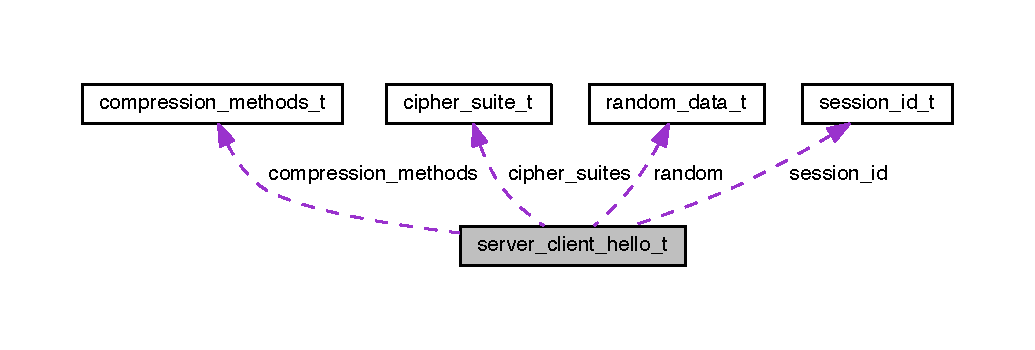
\includegraphics[width=350pt]{structserver__client__hello__t__coll__graph}
\end{center}
\end{figure}
\subsection*{Data Fields}
\begin{DoxyCompactItemize}
\item 
uint16\+\_\+t \hyperlink{structserver__client__hello__t_a5b4305b976c657bb4a056e00aeadb8ef}{T\+L\+S\+\_\+version}
\item 
\hyperlink{structrandom__data__t}{random\+\_\+data\+\_\+t} \hyperlink{structserver__client__hello__t_aefaae3d96978baaa21b9445a5728b4fe}{random}
\item 
\hyperlink{structsession__id__t}{session\+\_\+id\+\_\+t} \hyperlink{structserver__client__hello__t_a74379b0c9faddd3c3481e648a4ba2356}{session\+\_\+id}
\item 
\hyperlink{structcipher__suite__t}{cipher\+\_\+suite\+\_\+t} $\ast$ \hyperlink{structserver__client__hello__t_a545e2b09874bc2250aed603ef61820a6}{cipher\+\_\+suites}
\item 
uint16\+\_\+t \hyperlink{structserver__client__hello__t_a706adb2fc3f8fa8fe9bdd5793f32183e}{cipher\+\_\+suite\+\_\+len}
\item 
\hyperlink{structcompression__methods__t}{compression\+\_\+methods\+\_\+t} \hyperlink{structserver__client__hello__t_a08a470f144044c5ea244590f9ead8165}{compression\+\_\+methods}
\end{DoxyCompactItemize}


\subsection{Detailed Description}
Model a server/client hello message with all his field. Extension are not implemented yet. 

\subsection{Field Documentation}
\index{server\+\_\+client\+\_\+hello\+\_\+t@{server\+\_\+client\+\_\+hello\+\_\+t}!cipher\+\_\+suite\+\_\+len@{cipher\+\_\+suite\+\_\+len}}
\index{cipher\+\_\+suite\+\_\+len@{cipher\+\_\+suite\+\_\+len}!server\+\_\+client\+\_\+hello\+\_\+t@{server\+\_\+client\+\_\+hello\+\_\+t}}
\subsubsection[{\texorpdfstring{cipher\+\_\+suite\+\_\+len}{cipher_suite_len}}]{\setlength{\rightskip}{0pt plus 5cm}uint16\+\_\+t cipher\+\_\+suite\+\_\+len}\hypertarget{structserver__client__hello__t_a706adb2fc3f8fa8fe9bdd5793f32183e}{}\label{structserver__client__hello__t_a706adb2fc3f8fa8fe9bdd5793f32183e}
The space in byte used by the cipher suites. Each cipher suite need 2 byte for his id. 

Referenced by deserialize\+\_\+client\+\_\+server\+\_\+hello(), make\+\_\+client\+\_\+hello(), make\+\_\+server\+\_\+hello(), print\+\_\+hello(), and serialize\+\_\+client\+\_\+server\+\_\+hello().

\index{server\+\_\+client\+\_\+hello\+\_\+t@{server\+\_\+client\+\_\+hello\+\_\+t}!cipher\+\_\+suites@{cipher\+\_\+suites}}
\index{cipher\+\_\+suites@{cipher\+\_\+suites}!server\+\_\+client\+\_\+hello\+\_\+t@{server\+\_\+client\+\_\+hello\+\_\+t}}
\subsubsection[{\texorpdfstring{cipher\+\_\+suites}{cipher_suites}}]{\setlength{\rightskip}{0pt plus 5cm}{\bf cipher\+\_\+suite\+\_\+t}$\ast$ cipher\+\_\+suites}\hypertarget{structserver__client__hello__t_a545e2b09874bc2250aed603ef61820a6}{}\label{structserver__client__hello__t_a545e2b09874bc2250aed603ef61820a6}
For the client hello this is list of supported cipher suite by client. For server hello it contains only one cipher suite. 

Referenced by deserialize\+\_\+client\+\_\+server\+\_\+hello(), free\+\_\+hello(), make\+\_\+client\+\_\+hello(), make\+\_\+server\+\_\+hello(), on\+Packet\+Receive(), print\+\_\+hello(), and serialize\+\_\+client\+\_\+server\+\_\+hello().

\index{server\+\_\+client\+\_\+hello\+\_\+t@{server\+\_\+client\+\_\+hello\+\_\+t}!compression\+\_\+methods@{compression\+\_\+methods}}
\index{compression\+\_\+methods@{compression\+\_\+methods}!server\+\_\+client\+\_\+hello\+\_\+t@{server\+\_\+client\+\_\+hello\+\_\+t}}
\subsubsection[{\texorpdfstring{compression\+\_\+methods}{compression_methods}}]{\setlength{\rightskip}{0pt plus 5cm}{\bf compression\+\_\+methods\+\_\+t} compression\+\_\+methods}\hypertarget{structserver__client__hello__t_a08a470f144044c5ea244590f9ead8165}{}\label{structserver__client__hello__t_a08a470f144044c5ea244590f9ead8165}
Compression struct 

Referenced by deserialize\+\_\+client\+\_\+server\+\_\+hello(), free\+\_\+hello(), make\+\_\+hello(), and serialize\+\_\+client\+\_\+server\+\_\+hello().

\index{server\+\_\+client\+\_\+hello\+\_\+t@{server\+\_\+client\+\_\+hello\+\_\+t}!random@{random}}
\index{random@{random}!server\+\_\+client\+\_\+hello\+\_\+t@{server\+\_\+client\+\_\+hello\+\_\+t}}
\subsubsection[{\texorpdfstring{random}{random}}]{\setlength{\rightskip}{0pt plus 5cm}{\bf random\+\_\+data\+\_\+t} random}\hypertarget{structserver__client__hello__t_aefaae3d96978baaa21b9445a5728b4fe}{}\label{structserver__client__hello__t_aefaae3d96978baaa21b9445a5728b4fe}
Random struct\+: U\+N\+IX timestamp, random stream 

Referenced by deserialize\+\_\+client\+\_\+server\+\_\+hello(), make\+\_\+client\+\_\+hello(), make\+\_\+hello(), make\+\_\+server\+\_\+hello(), on\+Packet\+Receive(), print\+\_\+hello(), and serialize\+\_\+client\+\_\+server\+\_\+hello().

\index{server\+\_\+client\+\_\+hello\+\_\+t@{server\+\_\+client\+\_\+hello\+\_\+t}!session\+\_\+id@{session\+\_\+id}}
\index{session\+\_\+id@{session\+\_\+id}!server\+\_\+client\+\_\+hello\+\_\+t@{server\+\_\+client\+\_\+hello\+\_\+t}}
\subsubsection[{\texorpdfstring{session\+\_\+id}{session_id}}]{\setlength{\rightskip}{0pt plus 5cm}{\bf session\+\_\+id\+\_\+t} session\+\_\+id}\hypertarget{structserver__client__hello__t_a74379b0c9faddd3c3481e648a4ba2356}{}\label{structserver__client__hello__t_a74379b0c9faddd3c3481e648a4ba2356}
Session struct\+: session id, session length 

Referenced by free\+\_\+hello(), make\+\_\+hello(), print\+\_\+hello(), and serialize\+\_\+client\+\_\+server\+\_\+hello().

\index{server\+\_\+client\+\_\+hello\+\_\+t@{server\+\_\+client\+\_\+hello\+\_\+t}!T\+L\+S\+\_\+version@{T\+L\+S\+\_\+version}}
\index{T\+L\+S\+\_\+version@{T\+L\+S\+\_\+version}!server\+\_\+client\+\_\+hello\+\_\+t@{server\+\_\+client\+\_\+hello\+\_\+t}}
\subsubsection[{\texorpdfstring{T\+L\+S\+\_\+version}{TLS_version}}]{\setlength{\rightskip}{0pt plus 5cm}uint16\+\_\+t {\bf T\+L\+S\+\_\+version}}\hypertarget{structserver__client__hello__t_a5b4305b976c657bb4a056e00aeadb8ef}{}\label{structserver__client__hello__t_a5b4305b976c657bb4a056e00aeadb8ef}
T\+LS version 

Referenced by deserialize\+\_\+client\+\_\+server\+\_\+hello(), make\+\_\+client\+\_\+hello(), make\+\_\+server\+\_\+hello(), on\+Packet\+Receive(), print\+\_\+hello(), and serialize\+\_\+client\+\_\+server\+\_\+hello().



The documentation for this struct was generated from the following file\+:\begin{DoxyCompactItemize}
\item 
include/\+Handshake\+Messages/\hyperlink{_server_client_hello_8h}{Server\+Client\+Hello.\+h}\end{DoxyCompactItemize}

\hypertarget{structsession__id__t}{}\section{session\+\_\+id\+\_\+t Struct Reference}
\label{structsession__id__t}\index{session\+\_\+id\+\_\+t@{session\+\_\+id\+\_\+t}}


{\ttfamily \#include $<$Server\+Client\+Hello.\+h$>$}

\subsection*{Data Fields}
\begin{DoxyCompactItemize}
\item 
uint8\+\_\+t \hyperlink{structsession__id__t_a9215daa8dba2536b15b9029e18017c3a}{session\+\_\+lenght}
\item 
unsigned char $\ast$ \hyperlink{structsession__id__t_a16b10327d41aa891822609659111d1a1}{session\+\_\+id}
\end{DoxyCompactItemize}


\subsection{Field Documentation}
\index{session\+\_\+id\+\_\+t@{session\+\_\+id\+\_\+t}!session\+\_\+id@{session\+\_\+id}}
\index{session\+\_\+id@{session\+\_\+id}!session\+\_\+id\+\_\+t@{session\+\_\+id\+\_\+t}}
\subsubsection[{\texorpdfstring{session\+\_\+id}{session_id}}]{\setlength{\rightskip}{0pt plus 5cm}unsigned char$\ast$ session\+\_\+id}\hypertarget{structsession__id__t_a16b10327d41aa891822609659111d1a1}{}\label{structsession__id__t_a16b10327d41aa891822609659111d1a1}


Referenced by deserialize\+\_\+client\+\_\+server\+\_\+hello(), free\+\_\+hello(), make\+\_\+client\+\_\+hello(), make\+\_\+server\+\_\+hello(), print\+\_\+hello(), and serialize\+\_\+client\+\_\+server\+\_\+hello().

\index{session\+\_\+id\+\_\+t@{session\+\_\+id\+\_\+t}!session\+\_\+lenght@{session\+\_\+lenght}}
\index{session\+\_\+lenght@{session\+\_\+lenght}!session\+\_\+id\+\_\+t@{session\+\_\+id\+\_\+t}}
\subsubsection[{\texorpdfstring{session\+\_\+lenght}{session_lenght}}]{\setlength{\rightskip}{0pt plus 5cm}uint8\+\_\+t session\+\_\+lenght}\hypertarget{structsession__id__t_a9215daa8dba2536b15b9029e18017c3a}{}\label{structsession__id__t_a9215daa8dba2536b15b9029e18017c3a}


Referenced by deserialize\+\_\+client\+\_\+server\+\_\+hello(), make\+\_\+client\+\_\+hello(), make\+\_\+server\+\_\+hello(), print\+\_\+hello(), and serialize\+\_\+client\+\_\+server\+\_\+hello().



The documentation for this struct was generated from the following file\+:\begin{DoxyCompactItemize}
\item 
/\+Users/\+Darka/\+Dropbox/\+U\+N\+I\+T\+N/\+Advanced\+Programming/\+Project/include/\+Handshake\+Messages/\hyperlink{_server_client_hello_8h}{Server\+Client\+Hello.\+h}\end{DoxyCompactItemize}

\hypertarget{struct_t_l_s__parameters__t}{}\section{T\+L\+S\+\_\+parameters\+\_\+t Struct Reference}
\label{struct_t_l_s__parameters__t}\index{T\+L\+S\+\_\+parameters\+\_\+t@{T\+L\+S\+\_\+parameters\+\_\+t}}


{\ttfamily \#include $<$T\+L\+S.\+h$>$}

\subsection*{Data Fields}
\begin{DoxyCompactItemize}
\item 
uint16\+\_\+t \hyperlink{struct_t_l_s__parameters__t_a8fd63193690a09b75e0aaf9b971ed3df}{tls\+\_\+version}
\item 
uint16\+\_\+t \hyperlink{struct_t_l_s__parameters__t_a7876cd7f12771bb13dfd180e2d74e02b}{previous\+\_\+state}
\item 
\hyperlink{structcipher__suite__t}{cipher\+\_\+suite\+\_\+t} \hyperlink{struct_t_l_s__parameters__t_af1d8ebe57a775be2b91550dbcacb2a58}{cipher\+\_\+suite}
\item 
unsigned char \hyperlink{struct_t_l_s__parameters__t_adbdca8d573a8e073ef16bf14229fb4c9}{client\+\_\+random} \mbox{[}32\mbox{]}
\item 
unsigned char \hyperlink{struct_t_l_s__parameters__t_a9159f146fbc286a8b55f4aa83396ae2f}{server\+\_\+random} \mbox{[}32\mbox{]}
\item 
\hyperlink{_server_client_key_exchange_8h_a0e7e73056ef40d5a7b303b385dee59cd}{server\+\_\+key\+\_\+exchange\+\_\+t} $\ast$ \hyperlink{struct_t_l_s__parameters__t_ad79527a4a6a3547cc16f0fb569767d9d}{server\+\_\+key\+\_\+ex}
\item 
unsigned char $\ast$ \hyperlink{struct_t_l_s__parameters__t_a68c2015df5cb7259aa1abdee33c8e6f3}{master\+\_\+secret}
\item 
int \hyperlink{struct_t_l_s__parameters__t_a7112487b636ca7921055d94ae02478fe}{master\+\_\+secret\+\_\+len}
\item 
unsigned char $\ast$ \hyperlink{struct_t_l_s__parameters__t_ac6734c87e703c22f7d34f71ca116d005}{handshake\+\_\+messages}
\item 
int \hyperlink{struct_t_l_s__parameters__t_afbdbb7d32255aef8951f95ccc44957fc}{handshake\+\_\+messages\+\_\+len}
\item 
X509 $\ast$ \hyperlink{struct_t_l_s__parameters__t_a832ae425d6bb6330e1e5e825ab85ac31}{server\+\_\+certificate}
\item 
B\+I\+G\+N\+UM $\ast$ \hyperlink{struct_t_l_s__parameters__t_aa7d109714bb4c1faa6aba18c0dd3dcae}{private\+\_\+key}
\end{DoxyCompactItemize}


\subsection{Detailed Description}
Struct \hyperlink{struct_t_l_s__parameters__t}{T\+L\+S\+\_\+parameters\+\_\+t} This struct contains all details about connection. It also contains data for complete the handshake. 

\subsection{Field Documentation}
\index{T\+L\+S\+\_\+parameters\+\_\+t@{T\+L\+S\+\_\+parameters\+\_\+t}!cipher\+\_\+suite@{cipher\+\_\+suite}}
\index{cipher\+\_\+suite@{cipher\+\_\+suite}!T\+L\+S\+\_\+parameters\+\_\+t@{T\+L\+S\+\_\+parameters\+\_\+t}}
\subsubsection[{\texorpdfstring{cipher\+\_\+suite}{cipher_suite}}]{\setlength{\rightskip}{0pt plus 5cm}{\bf cipher\+\_\+suite\+\_\+t} cipher\+\_\+suite}\hypertarget{struct_t_l_s__parameters__t_af1d8ebe57a775be2b91550dbcacb2a58}{}\label{struct_t_l_s__parameters__t_af1d8ebe57a775be2b91550dbcacb2a58}
The cipher suite used for handshake 

Referenced by compute\+\_\+set\+\_\+master\+\_\+key\+\_\+\+D\+H\+E(), compute\+\_\+set\+\_\+master\+\_\+key\+\_\+\+E\+C\+D\+H\+E(), compute\+\_\+set\+\_\+master\+\_\+key\+\_\+\+R\+S\+A(), do\+\_\+handshake(), make\+\_\+certificate(), make\+\_\+client\+\_\+key\+\_\+exchange(), make\+\_\+\+D\+H\+E\+\_\+client\+\_\+key\+\_\+exchange(), make\+\_\+\+D\+H\+E\+\_\+server\+\_\+key\+\_\+exchange(), make\+\_\+\+E\+C\+D\+H\+E\+\_\+client\+\_\+key\+\_\+exchange(), make\+\_\+\+E\+C\+D\+H\+E\+\_\+server\+\_\+key\+\_\+exchange(), make\+\_\+finished\+\_\+message(), make\+\_\+\+R\+S\+A\+\_\+client\+\_\+key\+\_\+exchange(), make\+\_\+server\+\_\+hello(), make\+\_\+server\+\_\+key\+\_\+exchange(), and on\+Packet\+Receive().

\index{T\+L\+S\+\_\+parameters\+\_\+t@{T\+L\+S\+\_\+parameters\+\_\+t}!client\+\_\+random@{client\+\_\+random}}
\index{client\+\_\+random@{client\+\_\+random}!T\+L\+S\+\_\+parameters\+\_\+t@{T\+L\+S\+\_\+parameters\+\_\+t}}
\subsubsection[{\texorpdfstring{client\+\_\+random}{client_random}}]{\setlength{\rightskip}{0pt plus 5cm}unsigned char client\+\_\+random\mbox{[}32\mbox{]}}\hypertarget{struct_t_l_s__parameters__t_adbdca8d573a8e073ef16bf14229fb4c9}{}\label{struct_t_l_s__parameters__t_adbdca8d573a8e073ef16bf14229fb4c9}
Client random, include the unix time stamp 

Referenced by compute\+\_\+set\+\_\+master\+\_\+key\+\_\+\+D\+H\+E(), compute\+\_\+set\+\_\+master\+\_\+key\+\_\+\+E\+C\+D\+H\+E(), compute\+\_\+set\+\_\+master\+\_\+key\+\_\+\+R\+S\+A(), do\+\_\+handshake(), make\+\_\+\+D\+H\+E\+\_\+client\+\_\+key\+\_\+exchange(), make\+\_\+\+D\+H\+E\+\_\+server\+\_\+key\+\_\+exchange(), make\+\_\+\+E\+C\+D\+H\+E\+\_\+client\+\_\+key\+\_\+exchange(), make\+\_\+\+E\+C\+D\+H\+E\+\_\+server\+\_\+key\+\_\+exchange(), make\+\_\+\+R\+S\+A\+\_\+client\+\_\+key\+\_\+exchange(), and on\+Packet\+Receive().

\index{T\+L\+S\+\_\+parameters\+\_\+t@{T\+L\+S\+\_\+parameters\+\_\+t}!handshake\+\_\+messages@{handshake\+\_\+messages}}
\index{handshake\+\_\+messages@{handshake\+\_\+messages}!T\+L\+S\+\_\+parameters\+\_\+t@{T\+L\+S\+\_\+parameters\+\_\+t}}
\subsubsection[{\texorpdfstring{handshake\+\_\+messages}{handshake_messages}}]{\setlength{\rightskip}{0pt plus 5cm}unsigned char$\ast$ handshake\+\_\+messages}\hypertarget{struct_t_l_s__parameters__t_ac6734c87e703c22f7d34f71ca116d005}{}\label{struct_t_l_s__parameters__t_ac6734c87e703c22f7d34f71ca116d005}
The backup of handshake messages exchanged during handshake 

Referenced by backup\+\_\+handshake(), do\+\_\+handshake(), main(), and make\+\_\+finished\+\_\+message().

\index{T\+L\+S\+\_\+parameters\+\_\+t@{T\+L\+S\+\_\+parameters\+\_\+t}!handshake\+\_\+messages\+\_\+len@{handshake\+\_\+messages\+\_\+len}}
\index{handshake\+\_\+messages\+\_\+len@{handshake\+\_\+messages\+\_\+len}!T\+L\+S\+\_\+parameters\+\_\+t@{T\+L\+S\+\_\+parameters\+\_\+t}}
\subsubsection[{\texorpdfstring{handshake\+\_\+messages\+\_\+len}{handshake_messages_len}}]{\setlength{\rightskip}{0pt plus 5cm}int handshake\+\_\+messages\+\_\+len}\hypertarget{struct_t_l_s__parameters__t_afbdbb7d32255aef8951f95ccc44957fc}{}\label{struct_t_l_s__parameters__t_afbdbb7d32255aef8951f95ccc44957fc}
Backup stream length 

Referenced by backup\+\_\+handshake(), and make\+\_\+finished\+\_\+message().

\index{T\+L\+S\+\_\+parameters\+\_\+t@{T\+L\+S\+\_\+parameters\+\_\+t}!master\+\_\+secret@{master\+\_\+secret}}
\index{master\+\_\+secret@{master\+\_\+secret}!T\+L\+S\+\_\+parameters\+\_\+t@{T\+L\+S\+\_\+parameters\+\_\+t}}
\subsubsection[{\texorpdfstring{master\+\_\+secret}{master_secret}}]{\setlength{\rightskip}{0pt plus 5cm}unsigned char$\ast$ master\+\_\+secret}\hypertarget{struct_t_l_s__parameters__t_a68c2015df5cb7259aa1abdee33c8e6f3}{}\label{struct_t_l_s__parameters__t_a68c2015df5cb7259aa1abdee33c8e6f3}
Session master secret 

Referenced by compute\+\_\+set\+\_\+master\+\_\+key\+\_\+\+D\+H\+E(), compute\+\_\+set\+\_\+master\+\_\+key\+\_\+\+E\+C\+D\+H\+E(), compute\+\_\+set\+\_\+master\+\_\+key\+\_\+\+R\+S\+A(), do\+\_\+handshake(), make\+\_\+\+D\+H\+E\+\_\+client\+\_\+key\+\_\+exchange(), make\+\_\+\+E\+C\+D\+H\+E\+\_\+client\+\_\+key\+\_\+exchange(), make\+\_\+finished\+\_\+message(), and make\+\_\+\+R\+S\+A\+\_\+client\+\_\+key\+\_\+exchange().

\index{T\+L\+S\+\_\+parameters\+\_\+t@{T\+L\+S\+\_\+parameters\+\_\+t}!master\+\_\+secret\+\_\+len@{master\+\_\+secret\+\_\+len}}
\index{master\+\_\+secret\+\_\+len@{master\+\_\+secret\+\_\+len}!T\+L\+S\+\_\+parameters\+\_\+t@{T\+L\+S\+\_\+parameters\+\_\+t}}
\subsubsection[{\texorpdfstring{master\+\_\+secret\+\_\+len}{master_secret_len}}]{\setlength{\rightskip}{0pt plus 5cm}int master\+\_\+secret\+\_\+len}\hypertarget{struct_t_l_s__parameters__t_a7112487b636ca7921055d94ae02478fe}{}\label{struct_t_l_s__parameters__t_a7112487b636ca7921055d94ae02478fe}
Master secret length 

Referenced by compute\+\_\+set\+\_\+master\+\_\+key\+\_\+\+D\+H\+E(), compute\+\_\+set\+\_\+master\+\_\+key\+\_\+\+E\+C\+D\+H\+E(), compute\+\_\+set\+\_\+master\+\_\+key\+\_\+\+R\+S\+A(), do\+\_\+handshake(), make\+\_\+\+D\+H\+E\+\_\+client\+\_\+key\+\_\+exchange(), make\+\_\+\+E\+C\+D\+H\+E\+\_\+client\+\_\+key\+\_\+exchange(), make\+\_\+finished\+\_\+message(), and make\+\_\+\+R\+S\+A\+\_\+client\+\_\+key\+\_\+exchange().

\index{T\+L\+S\+\_\+parameters\+\_\+t@{T\+L\+S\+\_\+parameters\+\_\+t}!previous\+\_\+state@{previous\+\_\+state}}
\index{previous\+\_\+state@{previous\+\_\+state}!T\+L\+S\+\_\+parameters\+\_\+t@{T\+L\+S\+\_\+parameters\+\_\+t}}
\subsubsection[{\texorpdfstring{previous\+\_\+state}{previous_state}}]{\setlength{\rightskip}{0pt plus 5cm}uint16\+\_\+t previous\+\_\+state}\hypertarget{struct_t_l_s__parameters__t_a7876cd7f12771bb13dfd180e2d74e02b}{}\label{struct_t_l_s__parameters__t_a7876cd7f12771bb13dfd180e2d74e02b}
Store the previous state in the handshake 

Referenced by do\+\_\+handshake(), and on\+Packet\+Receive().

\index{T\+L\+S\+\_\+parameters\+\_\+t@{T\+L\+S\+\_\+parameters\+\_\+t}!private\+\_\+key@{private\+\_\+key}}
\index{private\+\_\+key@{private\+\_\+key}!T\+L\+S\+\_\+parameters\+\_\+t@{T\+L\+S\+\_\+parameters\+\_\+t}}
\subsubsection[{\texorpdfstring{private\+\_\+key}{private_key}}]{\setlength{\rightskip}{0pt plus 5cm}B\+I\+G\+N\+UM$\ast$ private\+\_\+key}\hypertarget{struct_t_l_s__parameters__t_aa7d109714bb4c1faa6aba18c0dd3dcae}{}\label{struct_t_l_s__parameters__t_aa7d109714bb4c1faa6aba18c0dd3dcae}
The private key for the key exchange 

Referenced by compute\+\_\+set\+\_\+master\+\_\+key\+\_\+\+D\+H\+E(), compute\+\_\+set\+\_\+master\+\_\+key\+\_\+\+E\+C\+D\+H\+E(), make\+\_\+\+D\+H\+E\+\_\+server\+\_\+key\+\_\+exchange(), and make\+\_\+\+E\+C\+D\+H\+E\+\_\+server\+\_\+key\+\_\+exchange().

\index{T\+L\+S\+\_\+parameters\+\_\+t@{T\+L\+S\+\_\+parameters\+\_\+t}!server\+\_\+certificate@{server\+\_\+certificate}}
\index{server\+\_\+certificate@{server\+\_\+certificate}!T\+L\+S\+\_\+parameters\+\_\+t@{T\+L\+S\+\_\+parameters\+\_\+t}}
\subsubsection[{\texorpdfstring{server\+\_\+certificate}{server_certificate}}]{\setlength{\rightskip}{0pt plus 5cm}X509$\ast$ server\+\_\+certificate}\hypertarget{struct_t_l_s__parameters__t_a832ae425d6bb6330e1e5e825ab85ac31}{}\label{struct_t_l_s__parameters__t_a832ae425d6bb6330e1e5e825ab85ac31}
The server certificate 

Referenced by do\+\_\+handshake(), make\+\_\+certificate(), make\+\_\+\+D\+H\+E\+\_\+client\+\_\+key\+\_\+exchange(), make\+\_\+\+E\+C\+D\+H\+E\+\_\+client\+\_\+key\+\_\+exchange(), make\+\_\+\+R\+S\+A\+\_\+client\+\_\+key\+\_\+exchange(), and on\+Packet\+Receive().

\index{T\+L\+S\+\_\+parameters\+\_\+t@{T\+L\+S\+\_\+parameters\+\_\+t}!server\+\_\+key\+\_\+ex@{server\+\_\+key\+\_\+ex}}
\index{server\+\_\+key\+\_\+ex@{server\+\_\+key\+\_\+ex}!T\+L\+S\+\_\+parameters\+\_\+t@{T\+L\+S\+\_\+parameters\+\_\+t}}
\subsubsection[{\texorpdfstring{server\+\_\+key\+\_\+ex}{server_key_ex}}]{\setlength{\rightskip}{0pt plus 5cm}{\bf server\+\_\+key\+\_\+exchange\+\_\+t}$\ast$ server\+\_\+key\+\_\+ex}\hypertarget{struct_t_l_s__parameters__t_ad79527a4a6a3547cc16f0fb569767d9d}{}\label{struct_t_l_s__parameters__t_ad79527a4a6a3547cc16f0fb569767d9d}
Server key exchange message 

Referenced by compute\+\_\+set\+\_\+master\+\_\+key\+\_\+\+D\+H\+E(), compute\+\_\+set\+\_\+master\+\_\+key\+\_\+\+E\+C\+D\+H\+E(), do\+\_\+handshake(), make\+\_\+\+D\+H\+E\+\_\+client\+\_\+key\+\_\+exchange(), make\+\_\+\+D\+H\+E\+\_\+server\+\_\+key\+\_\+exchange(), make\+\_\+\+E\+C\+D\+H\+E\+\_\+client\+\_\+key\+\_\+exchange(), make\+\_\+\+E\+C\+D\+H\+E\+\_\+server\+\_\+key\+\_\+exchange(), make\+\_\+server\+\_\+key\+\_\+exchange(), and on\+Packet\+Receive().

\index{T\+L\+S\+\_\+parameters\+\_\+t@{T\+L\+S\+\_\+parameters\+\_\+t}!server\+\_\+random@{server\+\_\+random}}
\index{server\+\_\+random@{server\+\_\+random}!T\+L\+S\+\_\+parameters\+\_\+t@{T\+L\+S\+\_\+parameters\+\_\+t}}
\subsubsection[{\texorpdfstring{server\+\_\+random}{server_random}}]{\setlength{\rightskip}{0pt plus 5cm}unsigned char server\+\_\+random\mbox{[}32\mbox{]}}\hypertarget{struct_t_l_s__parameters__t_a9159f146fbc286a8b55f4aa83396ae2f}{}\label{struct_t_l_s__parameters__t_a9159f146fbc286a8b55f4aa83396ae2f}
Server random, include the unix time stamp 

Referenced by compute\+\_\+set\+\_\+master\+\_\+key\+\_\+\+D\+H\+E(), compute\+\_\+set\+\_\+master\+\_\+key\+\_\+\+E\+C\+D\+H\+E(), compute\+\_\+set\+\_\+master\+\_\+key\+\_\+\+R\+S\+A(), do\+\_\+handshake(), make\+\_\+\+D\+H\+E\+\_\+client\+\_\+key\+\_\+exchange(), make\+\_\+\+D\+H\+E\+\_\+server\+\_\+key\+\_\+exchange(), make\+\_\+\+E\+C\+D\+H\+E\+\_\+client\+\_\+key\+\_\+exchange(), make\+\_\+\+E\+C\+D\+H\+E\+\_\+server\+\_\+key\+\_\+exchange(), make\+\_\+\+R\+S\+A\+\_\+client\+\_\+key\+\_\+exchange(), make\+\_\+server\+\_\+hello(), and on\+Packet\+Receive().

\index{T\+L\+S\+\_\+parameters\+\_\+t@{T\+L\+S\+\_\+parameters\+\_\+t}!tls\+\_\+version@{tls\+\_\+version}}
\index{tls\+\_\+version@{tls\+\_\+version}!T\+L\+S\+\_\+parameters\+\_\+t@{T\+L\+S\+\_\+parameters\+\_\+t}}
\subsubsection[{\texorpdfstring{tls\+\_\+version}{tls_version}}]{\setlength{\rightskip}{0pt plus 5cm}uint16\+\_\+t tls\+\_\+version}\hypertarget{struct_t_l_s__parameters__t_a8fd63193690a09b75e0aaf9b971ed3df}{}\label{struct_t_l_s__parameters__t_a8fd63193690a09b75e0aaf9b971ed3df}
The T\+LS version 

Referenced by make\+\_\+\+R\+S\+A\+\_\+client\+\_\+key\+\_\+exchange(), and on\+Packet\+Receive().



The documentation for this struct was generated from the following file\+:\begin{DoxyCompactItemize}
\item 
/\+Users/\+Darka/\+Dropbox/\+U\+N\+I\+T\+N/\+Advanced\+Programming/\+Project/include/\hyperlink{_t_l_s_8h}{T\+L\+S.\+h}\end{DoxyCompactItemize}

\chapter{File Documentation}
\hypertarget{_crypto_8h}{}\section{/\+Users/\+Darka/\+Dropbox/\+U\+N\+I\+T\+N/\+Advanced\+Programming/\+Project/include/\+Crypto.h File Reference}
\label{_crypto_8h}\index{/\+Users/\+Darka/\+Dropbox/\+U\+N\+I\+T\+N/\+Advanced\+Programming/\+Project/include/\+Crypto.\+h@{/\+Users/\+Darka/\+Dropbox/\+U\+N\+I\+T\+N/\+Advanced\+Programming/\+Project/include/\+Crypto.\+h}}
{\ttfamily \#include $<$stdio.\+h$>$}\\*
{\ttfamily \#include $<$stdlib.\+h$>$}\\*
{\ttfamily \#include $<$string.\+h$>$}\\*
{\ttfamily \#include $<$openssl/rand.\+h$>$}\\*
{\ttfamily \#include $<$openssl/pem.\+h$>$}\\*
{\ttfamily \#include $<$openssl/rsa.\+h$>$}\\*
{\ttfamily \#include \char`\"{}T\+L\+S\+Constants.\+h\char`\"{}}\\*
{\ttfamily \#include \char`\"{}Server\+Client\+Key\+Exchange.\+h\char`\"{}}\\*
\subsection*{Functions}
\begin{DoxyCompactItemize}
\item 
void \hyperlink{_crypto_8h_a14bb82638713f9cf8778b58d6d64e33d}{P\+RF} (const E\+V\+P\+\_\+\+MD $\ast$hash, unsigned char $\ast$secret, int secret\+\_\+len, char $\ast$label, unsigned char $\ast$seed, int seed\+\_\+len, int result\+\_\+len, unsigned char $\ast$$\ast$result)
\item 
int \hyperlink{_crypto_8h_aebef13db99f3bbd7e9e2c55df1aa65c9}{sign\+\_\+\+D\+H\+E\+\_\+server\+\_\+key\+\_\+ex} (unsigned char $\ast$client\+\_\+random, unsigned char $\ast$server\+\_\+random, \hyperlink{structdhe__server__key__exchange__t}{dhe\+\_\+server\+\_\+key\+\_\+exchange\+\_\+t} $\ast$server\+\_\+key\+\_\+ex, \hyperlink{_t_l_s_constants_8h_a433e2522c8a62ae4d8b1c91badefef50}{authentication\+\_\+algorithm} au)
\item 
int \hyperlink{_crypto_8h_afbf202296205717442436cd3838d6df7}{verify\+\_\+\+D\+H\+E\+\_\+server\+\_\+key\+\_\+ex\+\_\+sign} (X509 $\ast$certificate, unsigned char $\ast$client\+\_\+random, unsigned char $\ast$server\+\_\+random, \hyperlink{structdhe__server__key__exchange__t}{dhe\+\_\+server\+\_\+key\+\_\+exchange\+\_\+t} $\ast$server\+\_\+key\+\_\+ex, \hyperlink{_t_l_s_constants_8h_a433e2522c8a62ae4d8b1c91badefef50}{authentication\+\_\+algorithm} au)
\item 
int \hyperlink{_crypto_8h_abe36fc162d9170d061024842f7ec6b9d}{sign\+\_\+\+E\+C\+D\+H\+E\+\_\+server\+\_\+key\+\_\+ex} (unsigned char $\ast$client\+\_\+random, unsigned char $\ast$server\+\_\+random, \hyperlink{structecdhe__server__key__exchange__t}{ecdhe\+\_\+server\+\_\+key\+\_\+exchange\+\_\+t} $\ast$server\+\_\+key\+\_\+ex, \hyperlink{_t_l_s_constants_8h_a433e2522c8a62ae4d8b1c91badefef50}{authentication\+\_\+algorithm} au)
\item 
int \hyperlink{_crypto_8h_a5de0523f653b00816828961ba5cc990b}{verify\+\_\+\+E\+C\+D\+H\+E\+\_\+server\+\_\+key\+\_\+ex\+\_\+sign} (X509 $\ast$certificate, unsigned char $\ast$client\+\_\+random, unsigned char $\ast$server\+\_\+random, \hyperlink{structecdhe__server__key__exchange__t}{ecdhe\+\_\+server\+\_\+key\+\_\+exchange\+\_\+t} $\ast$server\+\_\+key\+\_\+ex, \hyperlink{_t_l_s_constants_8h_a433e2522c8a62ae4d8b1c91badefef50}{authentication\+\_\+algorithm} au)
\end{DoxyCompactItemize}


\subsection{Function Documentation}
\index{Crypto.\+h@{Crypto.\+h}!P\+RF@{P\+RF}}
\index{P\+RF@{P\+RF}!Crypto.\+h@{Crypto.\+h}}
\subsubsection[{\texorpdfstring{P\+R\+F(const E\+V\+P\+\_\+\+M\+D $\ast$hash, unsigned char $\ast$secret, int secret\+\_\+len, char $\ast$label, unsigned char $\ast$seed, int seed\+\_\+len, int result\+\_\+len, unsigned char $\ast$$\ast$result)}{PRF(const EVP_MD *hash, unsigned char *secret, int secret_len, char *label, unsigned char *seed, int seed_len, int result_len, unsigned char **result)}}]{\setlength{\rightskip}{0pt plus 5cm}void P\+RF (
\begin{DoxyParamCaption}
\item[{const E\+V\+P\+\_\+\+MD $\ast$}]{hash, }
\item[{unsigned char $\ast$}]{secret, }
\item[{int}]{secret\+\_\+len, }
\item[{char $\ast$}]{label, }
\item[{unsigned char $\ast$}]{seed, }
\item[{int}]{seed\+\_\+len, }
\item[{int}]{result\+\_\+len, }
\item[{unsigned char $\ast$$\ast$}]{result}
\end{DoxyParamCaption}
)}\hypertarget{_crypto_8h_a14bb82638713f9cf8778b58d6d64e33d}{}\label{_crypto_8h_a14bb82638713f9cf8778b58d6d64e33d}


Referenced by compute\+\_\+set\+\_\+master\+\_\+key\+\_\+\+D\+H\+E(), compute\+\_\+set\+\_\+master\+\_\+key\+\_\+\+E\+C\+D\+H\+E(), compute\+\_\+set\+\_\+master\+\_\+key\+\_\+\+R\+S\+A(), make\+\_\+\+D\+H\+E\+\_\+client\+\_\+key\+\_\+exchange(), make\+\_\+\+E\+C\+D\+H\+E\+\_\+client\+\_\+key\+\_\+exchange(), make\+\_\+finished\+\_\+message(), and make\+\_\+\+R\+S\+A\+\_\+client\+\_\+key\+\_\+exchange().

\index{Crypto.\+h@{Crypto.\+h}!sign\+\_\+\+D\+H\+E\+\_\+server\+\_\+key\+\_\+ex@{sign\+\_\+\+D\+H\+E\+\_\+server\+\_\+key\+\_\+ex}}
\index{sign\+\_\+\+D\+H\+E\+\_\+server\+\_\+key\+\_\+ex@{sign\+\_\+\+D\+H\+E\+\_\+server\+\_\+key\+\_\+ex}!Crypto.\+h@{Crypto.\+h}}
\subsubsection[{\texorpdfstring{sign\+\_\+\+D\+H\+E\+\_\+server\+\_\+key\+\_\+ex(unsigned char $\ast$client\+\_\+random, unsigned char $\ast$server\+\_\+random, dhe\+\_\+server\+\_\+key\+\_\+exchange\+\_\+t $\ast$server\+\_\+key\+\_\+ex, authentication\+\_\+algorithm au)}{sign_DHE_server_key_ex(unsigned char *client_random, unsigned char *server_random, dhe_server_key_exchange_t *server_key_ex, authentication_algorithm au)}}]{\setlength{\rightskip}{0pt plus 5cm}int sign\+\_\+\+D\+H\+E\+\_\+server\+\_\+key\+\_\+ex (
\begin{DoxyParamCaption}
\item[{unsigned char $\ast$}]{client\+\_\+random, }
\item[{unsigned char $\ast$}]{server\+\_\+random, }
\item[{{\bf dhe\+\_\+server\+\_\+key\+\_\+exchange\+\_\+t} $\ast$}]{server\+\_\+key\+\_\+ex, }
\item[{{\bf authentication\+\_\+algorithm}}]{au}
\end{DoxyParamCaption}
)}\hypertarget{_crypto_8h_aebef13db99f3bbd7e9e2c55df1aa65c9}{}\label{_crypto_8h_aebef13db99f3bbd7e9e2c55df1aa65c9}


Referenced by make\+\_\+\+D\+H\+E\+\_\+server\+\_\+key\+\_\+exchange().

\index{Crypto.\+h@{Crypto.\+h}!sign\+\_\+\+E\+C\+D\+H\+E\+\_\+server\+\_\+key\+\_\+ex@{sign\+\_\+\+E\+C\+D\+H\+E\+\_\+server\+\_\+key\+\_\+ex}}
\index{sign\+\_\+\+E\+C\+D\+H\+E\+\_\+server\+\_\+key\+\_\+ex@{sign\+\_\+\+E\+C\+D\+H\+E\+\_\+server\+\_\+key\+\_\+ex}!Crypto.\+h@{Crypto.\+h}}
\subsubsection[{\texorpdfstring{sign\+\_\+\+E\+C\+D\+H\+E\+\_\+server\+\_\+key\+\_\+ex(unsigned char $\ast$client\+\_\+random, unsigned char $\ast$server\+\_\+random, ecdhe\+\_\+server\+\_\+key\+\_\+exchange\+\_\+t $\ast$server\+\_\+key\+\_\+ex, authentication\+\_\+algorithm au)}{sign_ECDHE_server_key_ex(unsigned char *client_random, unsigned char *server_random, ecdhe_server_key_exchange_t *server_key_ex, authentication_algorithm au)}}]{\setlength{\rightskip}{0pt plus 5cm}int sign\+\_\+\+E\+C\+D\+H\+E\+\_\+server\+\_\+key\+\_\+ex (
\begin{DoxyParamCaption}
\item[{unsigned char $\ast$}]{client\+\_\+random, }
\item[{unsigned char $\ast$}]{server\+\_\+random, }
\item[{{\bf ecdhe\+\_\+server\+\_\+key\+\_\+exchange\+\_\+t} $\ast$}]{server\+\_\+key\+\_\+ex, }
\item[{{\bf authentication\+\_\+algorithm}}]{au}
\end{DoxyParamCaption}
)}\hypertarget{_crypto_8h_abe36fc162d9170d061024842f7ec6b9d}{}\label{_crypto_8h_abe36fc162d9170d061024842f7ec6b9d}


Referenced by make\+\_\+\+E\+C\+D\+H\+E\+\_\+server\+\_\+key\+\_\+exchange().

\index{Crypto.\+h@{Crypto.\+h}!verify\+\_\+\+D\+H\+E\+\_\+server\+\_\+key\+\_\+ex\+\_\+sign@{verify\+\_\+\+D\+H\+E\+\_\+server\+\_\+key\+\_\+ex\+\_\+sign}}
\index{verify\+\_\+\+D\+H\+E\+\_\+server\+\_\+key\+\_\+ex\+\_\+sign@{verify\+\_\+\+D\+H\+E\+\_\+server\+\_\+key\+\_\+ex\+\_\+sign}!Crypto.\+h@{Crypto.\+h}}
\subsubsection[{\texorpdfstring{verify\+\_\+\+D\+H\+E\+\_\+server\+\_\+key\+\_\+ex\+\_\+sign(\+X509 $\ast$certificate, unsigned char $\ast$client\+\_\+random, unsigned char $\ast$server\+\_\+random, dhe\+\_\+server\+\_\+key\+\_\+exchange\+\_\+t $\ast$server\+\_\+key\+\_\+ex, authentication\+\_\+algorithm au)}{verify_DHE_server_key_ex_sign(X509 *certificate, unsigned char *client_random, unsigned char *server_random, dhe_server_key_exchange_t *server_key_ex, authentication_algorithm au)}}]{\setlength{\rightskip}{0pt plus 5cm}int verify\+\_\+\+D\+H\+E\+\_\+server\+\_\+key\+\_\+ex\+\_\+sign (
\begin{DoxyParamCaption}
\item[{X509 $\ast$}]{certificate, }
\item[{unsigned char $\ast$}]{client\+\_\+random, }
\item[{unsigned char $\ast$}]{server\+\_\+random, }
\item[{{\bf dhe\+\_\+server\+\_\+key\+\_\+exchange\+\_\+t} $\ast$}]{server\+\_\+key\+\_\+ex, }
\item[{{\bf authentication\+\_\+algorithm}}]{au}
\end{DoxyParamCaption}
)}\hypertarget{_crypto_8h_afbf202296205717442436cd3838d6df7}{}\label{_crypto_8h_afbf202296205717442436cd3838d6df7}


Referenced by make\+\_\+\+D\+H\+E\+\_\+client\+\_\+key\+\_\+exchange().

\index{Crypto.\+h@{Crypto.\+h}!verify\+\_\+\+E\+C\+D\+H\+E\+\_\+server\+\_\+key\+\_\+ex\+\_\+sign@{verify\+\_\+\+E\+C\+D\+H\+E\+\_\+server\+\_\+key\+\_\+ex\+\_\+sign}}
\index{verify\+\_\+\+E\+C\+D\+H\+E\+\_\+server\+\_\+key\+\_\+ex\+\_\+sign@{verify\+\_\+\+E\+C\+D\+H\+E\+\_\+server\+\_\+key\+\_\+ex\+\_\+sign}!Crypto.\+h@{Crypto.\+h}}
\subsubsection[{\texorpdfstring{verify\+\_\+\+E\+C\+D\+H\+E\+\_\+server\+\_\+key\+\_\+ex\+\_\+sign(\+X509 $\ast$certificate, unsigned char $\ast$client\+\_\+random, unsigned char $\ast$server\+\_\+random, ecdhe\+\_\+server\+\_\+key\+\_\+exchange\+\_\+t $\ast$server\+\_\+key\+\_\+ex, authentication\+\_\+algorithm au)}{verify_ECDHE_server_key_ex_sign(X509 *certificate, unsigned char *client_random, unsigned char *server_random, ecdhe_server_key_exchange_t *server_key_ex, authentication_algorithm au)}}]{\setlength{\rightskip}{0pt plus 5cm}int verify\+\_\+\+E\+C\+D\+H\+E\+\_\+server\+\_\+key\+\_\+ex\+\_\+sign (
\begin{DoxyParamCaption}
\item[{X509 $\ast$}]{certificate, }
\item[{unsigned char $\ast$}]{client\+\_\+random, }
\item[{unsigned char $\ast$}]{server\+\_\+random, }
\item[{{\bf ecdhe\+\_\+server\+\_\+key\+\_\+exchange\+\_\+t} $\ast$}]{server\+\_\+key\+\_\+ex, }
\item[{{\bf authentication\+\_\+algorithm}}]{au}
\end{DoxyParamCaption}
)}\hypertarget{_crypto_8h_a5de0523f653b00816828961ba5cc990b}{}\label{_crypto_8h_a5de0523f653b00816828961ba5cc990b}


Referenced by make\+\_\+\+E\+C\+D\+H\+E\+\_\+client\+\_\+key\+\_\+exchange().


\hypertarget{_certificate_8h}{}\section{include/\+Handshake\+Messages/\+Certificate.h File Reference}
\label{_certificate_8h}\index{include/\+Handshake\+Messages/\+Certificate.\+h@{include/\+Handshake\+Messages/\+Certificate.\+h}}
{\ttfamily \#include $<$stdio.\+h$>$}\\*
{\ttfamily \#include $<$stdint.\+h$>$}\\*
{\ttfamily \#include $<$string.\+h$>$}\\*
{\ttfamily \#include $<$openssl/x509.\+h$>$}\\*
{\ttfamily \#include $<$openssl/pem.\+h$>$}\\*
{\ttfamily \#include \char`\"{}T\+L\+S\+Constants.\+h\char`\"{}}\\*
Include dependency graph for Certificate.\+h\+:\nopagebreak
\begin{figure}[H]
\begin{center}
\leavevmode
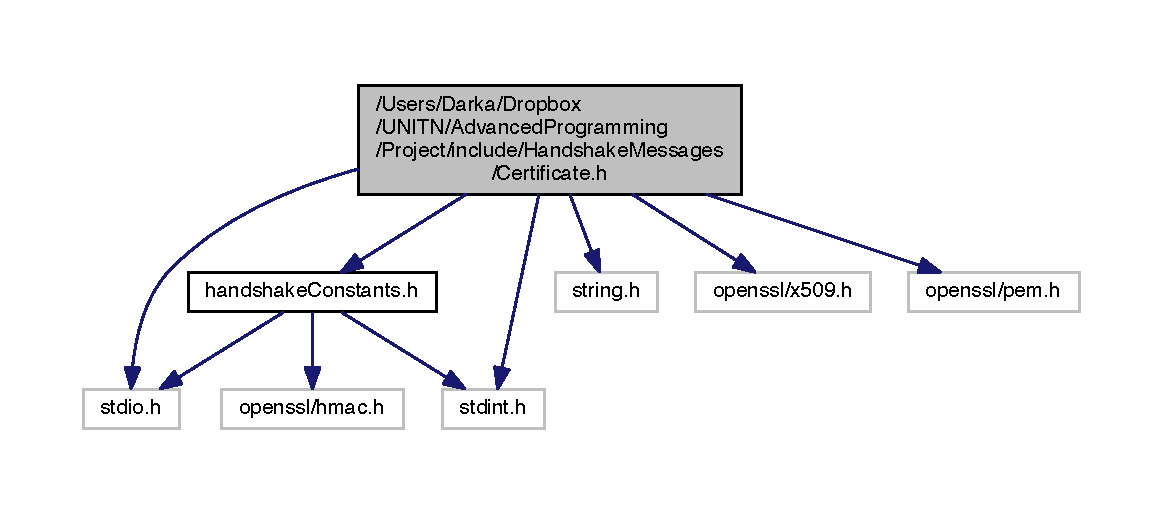
\includegraphics[width=350pt]{_certificate_8h__incl}
\end{center}
\end{figure}
This graph shows which files directly or indirectly include this file\+:\nopagebreak
\begin{figure}[H]
\begin{center}
\leavevmode
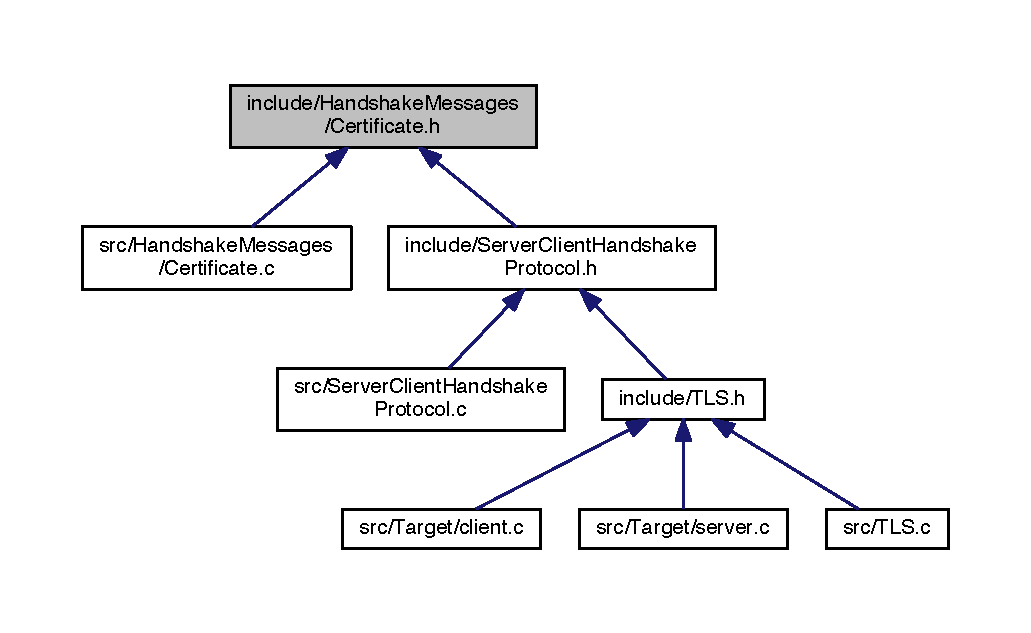
\includegraphics[width=350pt]{_certificate_8h__dep__incl}
\end{center}
\end{figure}
\subsection*{Data Structures}
\begin{DoxyCompactItemize}
\item 
struct \hyperlink{structcertificate__message__t}{certificate\+\_\+message\+\_\+t}
\end{DoxyCompactItemize}
\subsection*{Functions}
\begin{DoxyCompactItemize}
\item 
\hyperlink{structcertificate__message__t}{certificate\+\_\+message\+\_\+t} $\ast$ \hyperlink{_certificate_8h_a1eb2ef0668ed7bc45a2416b5b6a707f1}{make\+\_\+certificate\+\_\+message} (char $\ast$cert\+\_\+file\+\_\+name)
\item 
void \hyperlink{_certificate_8h_a0939aba653417f0b516a6d6a2a102b3d}{serialize\+\_\+certificate\+\_\+message} (\hyperlink{structcertificate__message__t}{certificate\+\_\+message\+\_\+t} $\ast$cert, unsigned char $\ast$$\ast$stream, uint32\+\_\+t $\ast$len)
\item 
\hyperlink{structcertificate__message__t}{certificate\+\_\+message\+\_\+t} $\ast$ \hyperlink{_certificate_8h_a5eca0d90b55f94993347dcd06ca0328e}{deserialize\+\_\+certificate\+\_\+message} (unsigned char $\ast$stream, uint32\+\_\+t len)
\item 
void \hyperlink{_certificate_8h_a47cd7cd727cb5ed51f41bf165585a386}{free\+\_\+certificate\+\_\+message} (\hyperlink{structcertificate__message__t}{certificate\+\_\+message\+\_\+t} $\ast$cert)
\end{DoxyCompactItemize}


\subsection{Detailed Description}
S\+S\+L/\+T\+LS Project

This file contains functions to manage the certificate message.

\begin{DoxyDate}{Date}
Created on 28/12/15. 
\end{DoxyDate}
\begin{DoxyCopyright}{Copyright}
Copyright © 2015 Alessandro Melloni, Andrea Francesco Vinci. All rights reserved. 
\end{DoxyCopyright}


\subsection{Function Documentation}
\index{Certificate.\+h@{Certificate.\+h}!deserialize\+\_\+certificate\+\_\+message@{deserialize\+\_\+certificate\+\_\+message}}
\index{deserialize\+\_\+certificate\+\_\+message@{deserialize\+\_\+certificate\+\_\+message}!Certificate.\+h@{Certificate.\+h}}
\subsubsection[{\texorpdfstring{deserialize\+\_\+certificate\+\_\+message(unsigned char $\ast$stream, uint32\+\_\+t len)}{deserialize_certificate_message(unsigned char *stream, uint32_t len)}}]{\setlength{\rightskip}{0pt plus 5cm}{\bf certificate\+\_\+message\+\_\+t}$\ast$ deserialize\+\_\+certificate\+\_\+message (
\begin{DoxyParamCaption}
\item[{unsigned char $\ast$}]{stream, }
\item[{uint32\+\_\+t}]{len}
\end{DoxyParamCaption}
)}\hypertarget{_certificate_8h_a5eca0d90b55f94993347dcd06ca0328e}{}\label{_certificate_8h_a5eca0d90b55f94993347dcd06ca0328e}
De-\/serialize a byte stream into a certificate\+\_\+message.


\begin{DoxyParams}{Parameters}
{\em stream} & the byte stream to de-\/serialize \\
\hline
{\em len} & the byte stream length \\
\hline
\end{DoxyParams}
\begin{DoxyReturn}{Returns}
the certificate\+\_\+message 
\end{DoxyReturn}


Referenced by on\+Packet\+Receive(), and print\+\_\+handshake().



Here is the caller graph for this function\+:
\nopagebreak
\begin{figure}[H]
\begin{center}
\leavevmode
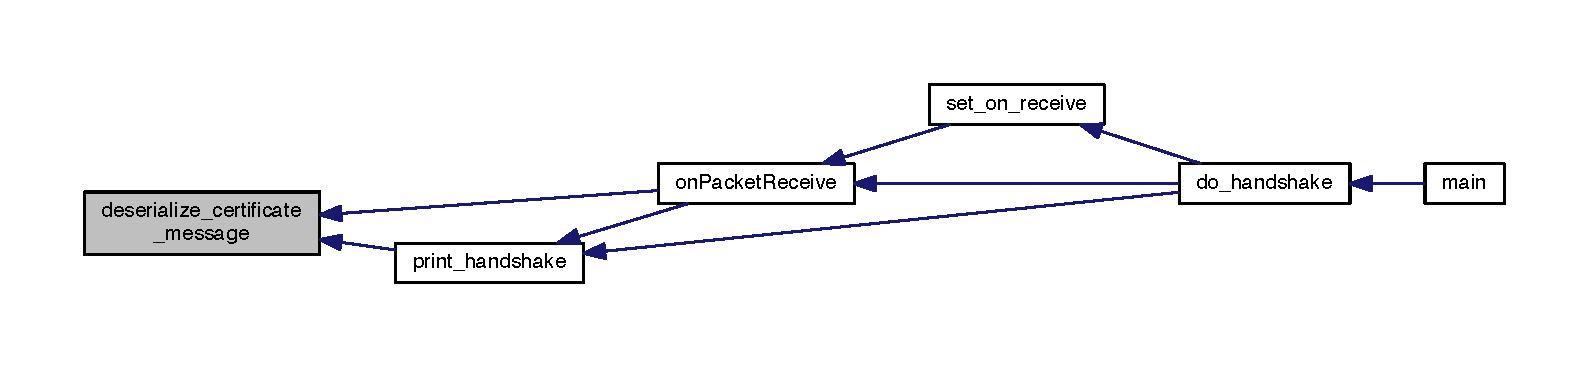
\includegraphics[width=350pt]{_certificate_8h_a5eca0d90b55f94993347dcd06ca0328e_icgraph}
\end{center}
\end{figure}


\index{Certificate.\+h@{Certificate.\+h}!free\+\_\+certificate\+\_\+message@{free\+\_\+certificate\+\_\+message}}
\index{free\+\_\+certificate\+\_\+message@{free\+\_\+certificate\+\_\+message}!Certificate.\+h@{Certificate.\+h}}
\subsubsection[{\texorpdfstring{free\+\_\+certificate\+\_\+message(certificate\+\_\+message\+\_\+t $\ast$cert)}{free_certificate_message(certificate_message_t *cert)}}]{\setlength{\rightskip}{0pt plus 5cm}void free\+\_\+certificate\+\_\+message (
\begin{DoxyParamCaption}
\item[{{\bf certificate\+\_\+message\+\_\+t} $\ast$}]{cert}
\end{DoxyParamCaption}
)}\hypertarget{_certificate_8h_a47cd7cd727cb5ed51f41bf165585a386}{}\label{_certificate_8h_a47cd7cd727cb5ed51f41bf165585a386}
Dealloc memory of certificate\+\_\+message


\begin{DoxyParams}{Parameters}
{\em cert} & the certificate message to deallocate \\
\hline
\end{DoxyParams}


Referenced by make\+\_\+certificate(), on\+Packet\+Receive(), and print\+\_\+handshake().



Here is the caller graph for this function\+:
\nopagebreak
\begin{figure}[H]
\begin{center}
\leavevmode
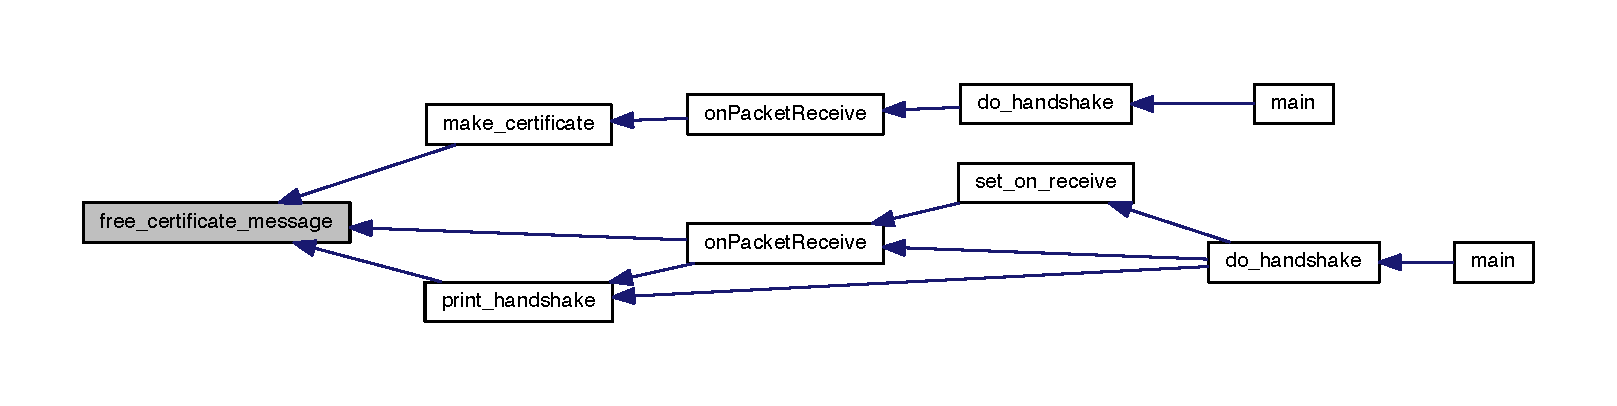
\includegraphics[width=350pt]{_certificate_8h_a47cd7cd727cb5ed51f41bf165585a386_icgraph}
\end{center}
\end{figure}


\index{Certificate.\+h@{Certificate.\+h}!make\+\_\+certificate\+\_\+message@{make\+\_\+certificate\+\_\+message}}
\index{make\+\_\+certificate\+\_\+message@{make\+\_\+certificate\+\_\+message}!Certificate.\+h@{Certificate.\+h}}
\subsubsection[{\texorpdfstring{make\+\_\+certificate\+\_\+message(char $\ast$cert\+\_\+file\+\_\+name)}{make_certificate_message(char *cert_file_name)}}]{\setlength{\rightskip}{0pt plus 5cm}{\bf certificate\+\_\+message\+\_\+t}$\ast$ make\+\_\+certificate\+\_\+message (
\begin{DoxyParamCaption}
\item[{char $\ast$}]{cert\+\_\+file\+\_\+name}
\end{DoxyParamCaption}
)}\hypertarget{_certificate_8h_a1eb2ef0668ed7bc45a2416b5b6a707f1}{}\label{_certificate_8h_a1eb2ef0668ed7bc45a2416b5b6a707f1}
Given the certificate file name create a certificate message struct that encapsulate it.


\begin{DoxyParams}{Parameters}
{\em cert\+\_\+file\+\_\+name} & certificate file name including path \\
\hline
\end{DoxyParams}
\begin{DoxyReturn}{Returns}
the certificate message struct 
\end{DoxyReturn}


Referenced by make\+\_\+certificate().



Here is the caller graph for this function\+:
\nopagebreak
\begin{figure}[H]
\begin{center}
\leavevmode
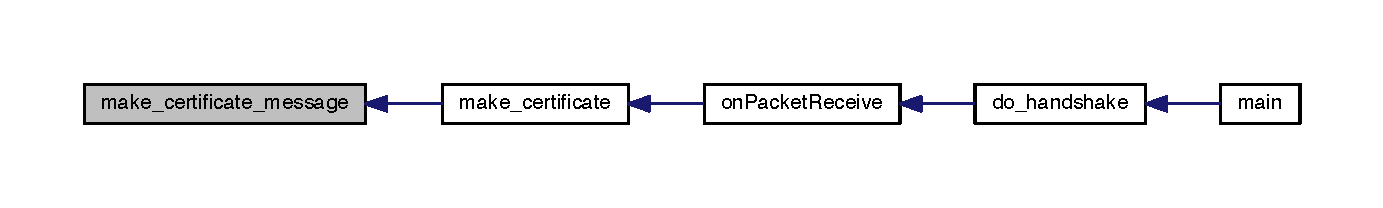
\includegraphics[width=350pt]{_certificate_8h_a1eb2ef0668ed7bc45a2416b5b6a707f1_icgraph}
\end{center}
\end{figure}


\index{Certificate.\+h@{Certificate.\+h}!serialize\+\_\+certificate\+\_\+message@{serialize\+\_\+certificate\+\_\+message}}
\index{serialize\+\_\+certificate\+\_\+message@{serialize\+\_\+certificate\+\_\+message}!Certificate.\+h@{Certificate.\+h}}
\subsubsection[{\texorpdfstring{serialize\+\_\+certificate\+\_\+message(certificate\+\_\+message\+\_\+t $\ast$cert, unsigned char $\ast$$\ast$stream, uint32\+\_\+t $\ast$len)}{serialize_certificate_message(certificate_message_t *cert, unsigned char **stream, uint32_t *len)}}]{\setlength{\rightskip}{0pt plus 5cm}void serialize\+\_\+certificate\+\_\+message (
\begin{DoxyParamCaption}
\item[{{\bf certificate\+\_\+message\+\_\+t} $\ast$}]{cert, }
\item[{unsigned char $\ast$$\ast$}]{stream, }
\item[{uint32\+\_\+t $\ast$}]{len}
\end{DoxyParamCaption}
)}\hypertarget{_certificate_8h_a0939aba653417f0b516a6d6a2a102b3d}{}\label{_certificate_8h_a0939aba653417f0b516a6d6a2a102b3d}
Serialize the certificate message into a byte stream


\begin{DoxyParams}{Parameters}
{\em cert} & the message to serialize \\
\hline
{\em stream} & the return stream. Must point to N\+U\+LL. \\
\hline
{\em len} & the stream length\\
\hline
\end{DoxyParams}
Serialize the certificate message into a byte stream


\begin{DoxyParams}{Parameters}
{\em cert} & the message to serialize \\
\hline
{\em stream} & the return stream. Must point to N\+U\+LL \\
\hline
{\em len} & the stream length \\
\hline
\end{DoxyParams}


Referenced by make\+\_\+certificate().



Here is the caller graph for this function\+:
\nopagebreak
\begin{figure}[H]
\begin{center}
\leavevmode
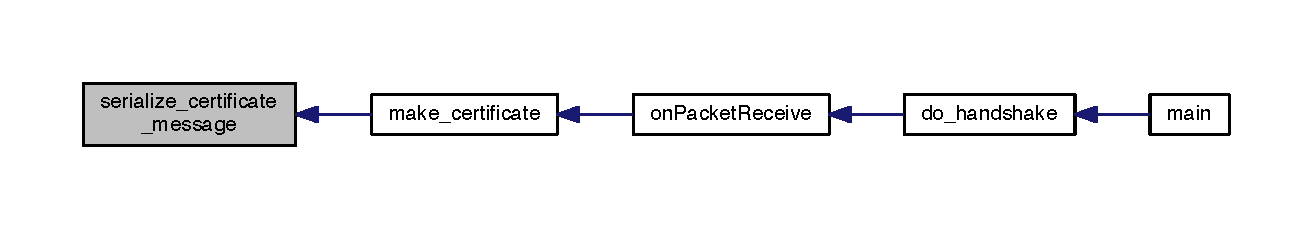
\includegraphics[width=350pt]{_certificate_8h_a0939aba653417f0b516a6d6a2a102b3d_icgraph}
\end{center}
\end{figure}



\hypertarget{_server_client_hello_8h}{}\section{include/\+Handshake\+Messages/\+Server\+Client\+Hello.h File Reference}
\label{_server_client_hello_8h}\index{include/\+Handshake\+Messages/\+Server\+Client\+Hello.\+h@{include/\+Handshake\+Messages/\+Server\+Client\+Hello.\+h}}
{\ttfamily \#include $<$stdio.\+h$>$}\\*
{\ttfamily \#include $<$stdint.\+h$>$}\\*
{\ttfamily \#include $<$time.\+h$>$}\\*
{\ttfamily \#include $<$stdlib.\+h$>$}\\*
{\ttfamily \#include $<$string.\+h$>$}\\*
{\ttfamily \#include $<$openssl/rand.\+h$>$}\\*
{\ttfamily \#include \char`\"{}T\+L\+S\+Constants.\+h\char`\"{}}\\*
Include dependency graph for Server\+Client\+Hello.\+h\+:
\nopagebreak
\begin{figure}[H]
\begin{center}
\leavevmode
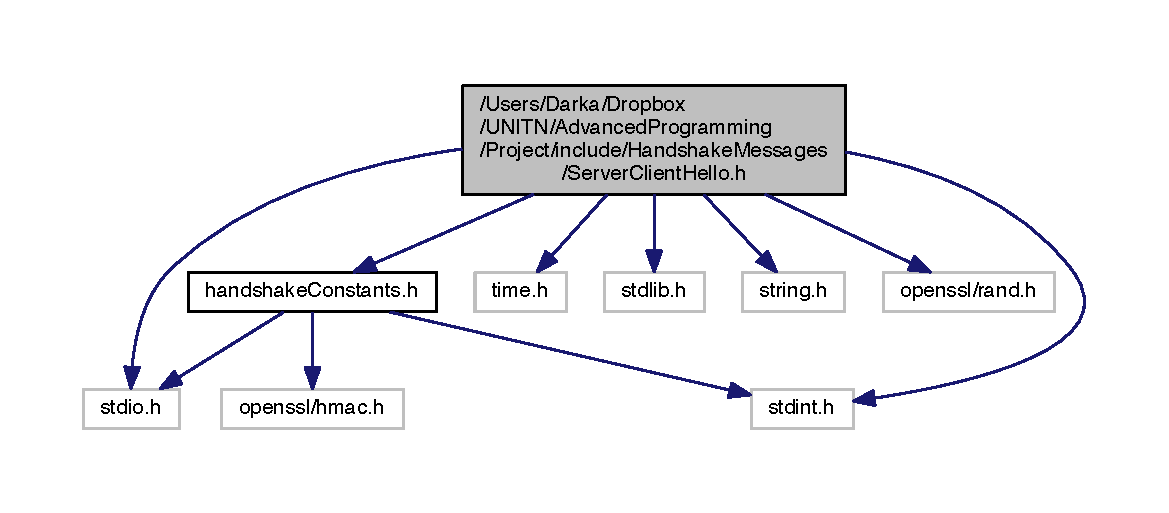
\includegraphics[width=350pt]{_server_client_hello_8h__incl}
\end{center}
\end{figure}
This graph shows which files directly or indirectly include this file\+:
\nopagebreak
\begin{figure}[H]
\begin{center}
\leavevmode
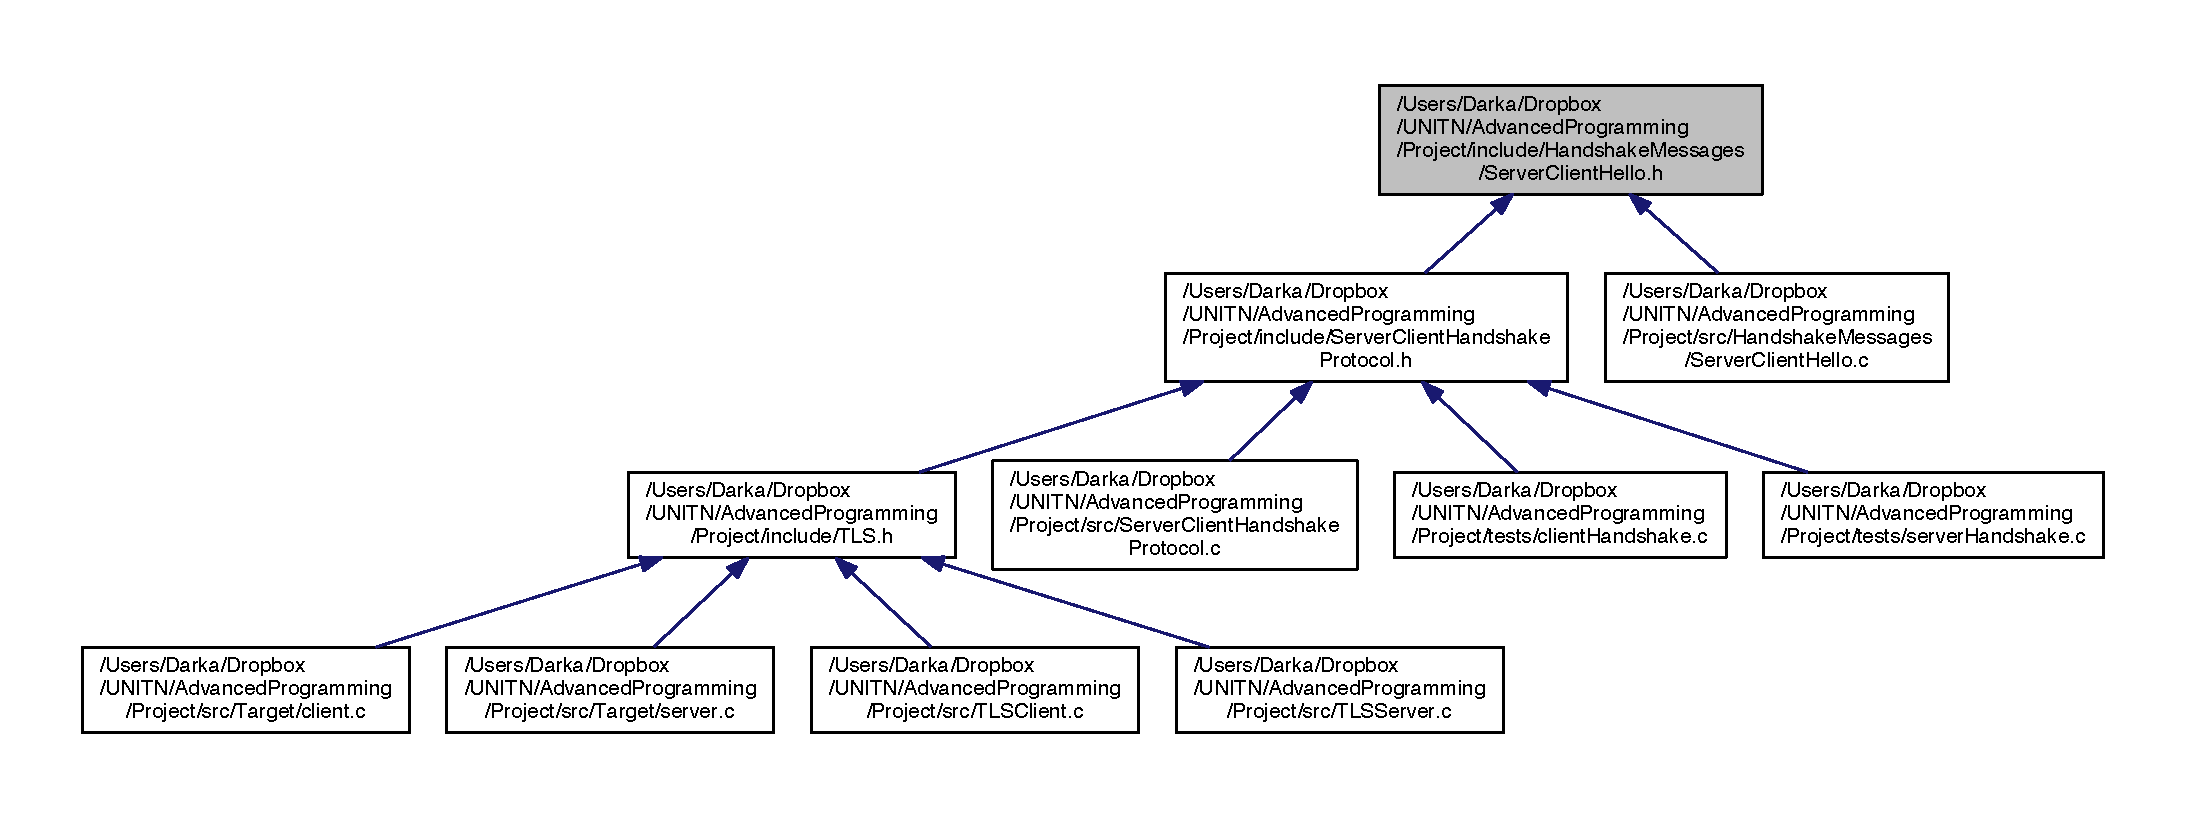
\includegraphics[width=350pt]{_server_client_hello_8h__dep__incl}
\end{center}
\end{figure}
\subsection*{Data Structures}
\begin{DoxyCompactItemize}
\item 
struct \hyperlink{structrandom__data__t}{random\+\_\+data\+\_\+t}
\item 
struct \hyperlink{structsession__id__t}{session\+\_\+id\+\_\+t}
\item 
struct \hyperlink{structcompression__methods__t}{compression\+\_\+methods\+\_\+t}
\item 
struct \hyperlink{structserver__client__hello__t}{server\+\_\+client\+\_\+hello\+\_\+t}
\end{DoxyCompactItemize}
\subsection*{Functions}
\begin{DoxyCompactItemize}
\item 
\hyperlink{structserver__client__hello__t}{server\+\_\+client\+\_\+hello\+\_\+t} $\ast$ \hyperlink{_server_client_hello_8h_a095e7c0597d66b5e4eb2097b8f28474a}{make\+\_\+hello} (\hyperlink{structsession__id__t}{session\+\_\+id\+\_\+t} session)
\item 
void \hyperlink{_server_client_hello_8h_a5d76fe55dc16550edc3604fcde33b8d0}{serialize\+\_\+client\+\_\+server\+\_\+hello} (\hyperlink{structserver__client__hello__t}{server\+\_\+client\+\_\+hello\+\_\+t} $\ast$hello, unsigned char $\ast$$\ast$stream, uint32\+\_\+t $\ast$stream\+Len, \hyperlink{_t_l_s_constants_8h_af21001704588d21e61c566facf69ec3d}{channel\+\_\+mode} mode)
\item 
\hyperlink{structserver__client__hello__t}{server\+\_\+client\+\_\+hello\+\_\+t} $\ast$ \hyperlink{_server_client_hello_8h_aaae83df7b184359cdb8f7f06931e7ad5}{deserialize\+\_\+client\+\_\+server\+\_\+hello} (unsigned char $\ast$stream, uint32\+\_\+t stream\+Len, \hyperlink{_t_l_s_constants_8h_af21001704588d21e61c566facf69ec3d}{channel\+\_\+mode} mode)
\item 
void \hyperlink{_server_client_hello_8h_aec7721cdc08398302cd7435054202117}{free\+\_\+hello} (\hyperlink{structserver__client__hello__t}{server\+\_\+client\+\_\+hello\+\_\+t} $\ast$h)
\item 
void \hyperlink{_server_client_hello_8h_aff8bed251595f5c51c0d1755799909ae}{print\+\_\+hello} (\hyperlink{structserver__client__hello__t}{server\+\_\+client\+\_\+hello\+\_\+t} $\ast$h)
\end{DoxyCompactItemize}


\subsection{Function Documentation}
\index{Server\+Client\+Hello.\+h@{Server\+Client\+Hello.\+h}!deserialize\+\_\+client\+\_\+server\+\_\+hello@{deserialize\+\_\+client\+\_\+server\+\_\+hello}}
\index{deserialize\+\_\+client\+\_\+server\+\_\+hello@{deserialize\+\_\+client\+\_\+server\+\_\+hello}!Server\+Client\+Hello.\+h@{Server\+Client\+Hello.\+h}}
\subsubsection[{\texorpdfstring{deserialize\+\_\+client\+\_\+server\+\_\+hello(unsigned char $\ast$stream, uint32\+\_\+t stream\+Len, channel\+\_\+mode mode)}{deserialize_client_server_hello(unsigned char *stream, uint32_t streamLen, channel_mode mode)}}]{\setlength{\rightskip}{0pt plus 5cm}{\bf server\+\_\+client\+\_\+hello\+\_\+t}$\ast$ deserialize\+\_\+client\+\_\+server\+\_\+hello (
\begin{DoxyParamCaption}
\item[{unsigned char $\ast$}]{stream, }
\item[{uint32\+\_\+t}]{stream\+Len, }
\item[{{\bf channel\+\_\+mode}}]{mode}
\end{DoxyParamCaption}
)}\hypertarget{_server_client_hello_8h_aaae83df7b184359cdb8f7f06931e7ad5}{}\label{_server_client_hello_8h_aaae83df7b184359cdb8f7f06931e7ad5}


Referenced by on\+Packet\+Receive(), and print\+\_\+handshake().



Here is the call graph for this function\+:\nopagebreak
\begin{figure}[H]
\begin{center}
\leavevmode
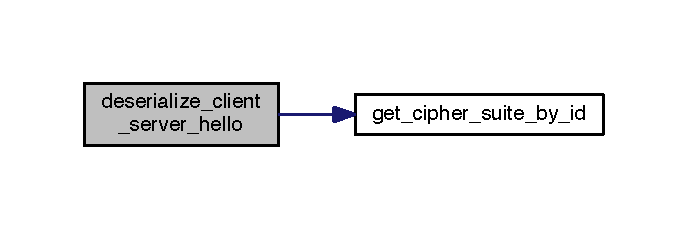
\includegraphics[width=330pt]{_server_client_hello_8h_aaae83df7b184359cdb8f7f06931e7ad5_cgraph}
\end{center}
\end{figure}




Here is the caller graph for this function\+:\nopagebreak
\begin{figure}[H]
\begin{center}
\leavevmode
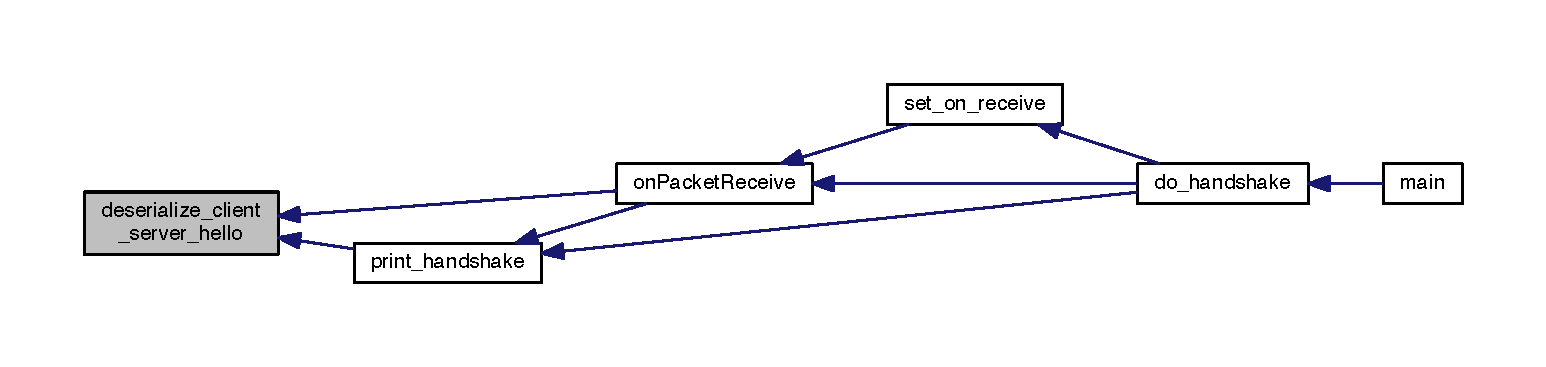
\includegraphics[width=350pt]{_server_client_hello_8h_aaae83df7b184359cdb8f7f06931e7ad5_icgraph}
\end{center}
\end{figure}


\index{Server\+Client\+Hello.\+h@{Server\+Client\+Hello.\+h}!free\+\_\+hello@{free\+\_\+hello}}
\index{free\+\_\+hello@{free\+\_\+hello}!Server\+Client\+Hello.\+h@{Server\+Client\+Hello.\+h}}
\subsubsection[{\texorpdfstring{free\+\_\+hello(server\+\_\+client\+\_\+hello\+\_\+t $\ast$h)}{free_hello(server_client_hello_t *h)}}]{\setlength{\rightskip}{0pt plus 5cm}void free\+\_\+hello (
\begin{DoxyParamCaption}
\item[{{\bf server\+\_\+client\+\_\+hello\+\_\+t} $\ast$}]{h}
\end{DoxyParamCaption}
)}\hypertarget{_server_client_hello_8h_aec7721cdc08398302cd7435054202117}{}\label{_server_client_hello_8h_aec7721cdc08398302cd7435054202117}


Referenced by make\+\_\+client\+\_\+hello(), make\+\_\+server\+\_\+hello(), on\+Packet\+Receive(), and print\+\_\+handshake().



Here is the caller graph for this function\+:\nopagebreak
\begin{figure}[H]
\begin{center}
\leavevmode
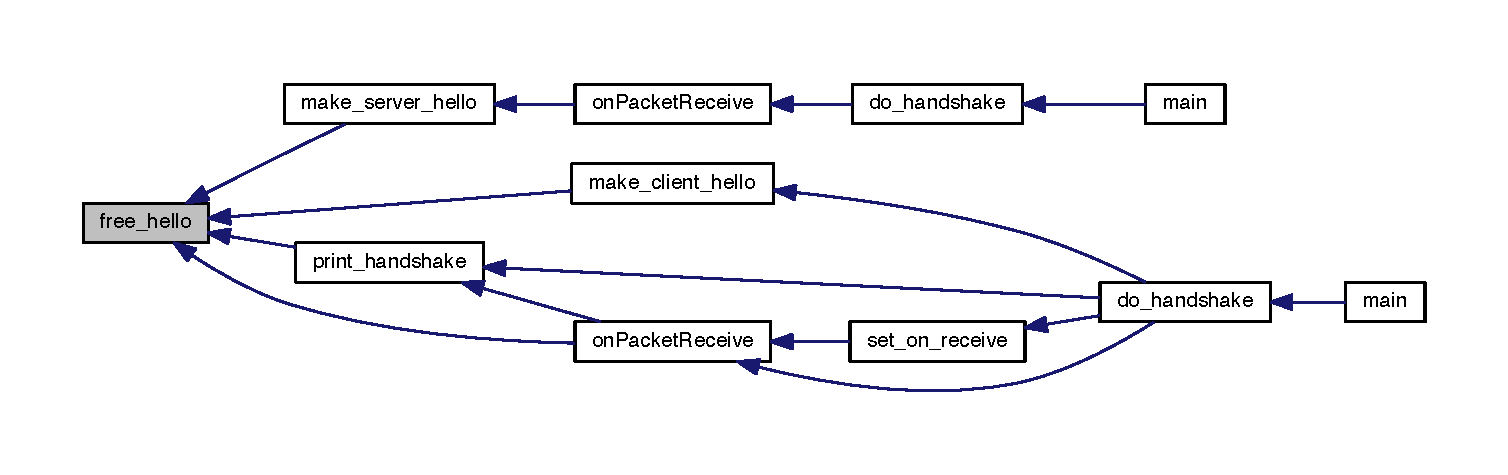
\includegraphics[width=350pt]{_server_client_hello_8h_aec7721cdc08398302cd7435054202117_icgraph}
\end{center}
\end{figure}


\index{Server\+Client\+Hello.\+h@{Server\+Client\+Hello.\+h}!make\+\_\+hello@{make\+\_\+hello}}
\index{make\+\_\+hello@{make\+\_\+hello}!Server\+Client\+Hello.\+h@{Server\+Client\+Hello.\+h}}
\subsubsection[{\texorpdfstring{make\+\_\+hello(session\+\_\+id\+\_\+t session)}{make_hello(session_id_t session)}}]{\setlength{\rightskip}{0pt plus 5cm}{\bf server\+\_\+client\+\_\+hello\+\_\+t}$\ast$ make\+\_\+hello (
\begin{DoxyParamCaption}
\item[{{\bf session\+\_\+id\+\_\+t}}]{session}
\end{DoxyParamCaption}
)}\hypertarget{_server_client_hello_8h_a095e7c0597d66b5e4eb2097b8f28474a}{}\label{_server_client_hello_8h_a095e7c0597d66b5e4eb2097b8f28474a}


Referenced by make\+\_\+client\+\_\+hello(), and make\+\_\+server\+\_\+hello().



Here is the caller graph for this function\+:\nopagebreak
\begin{figure}[H]
\begin{center}
\leavevmode
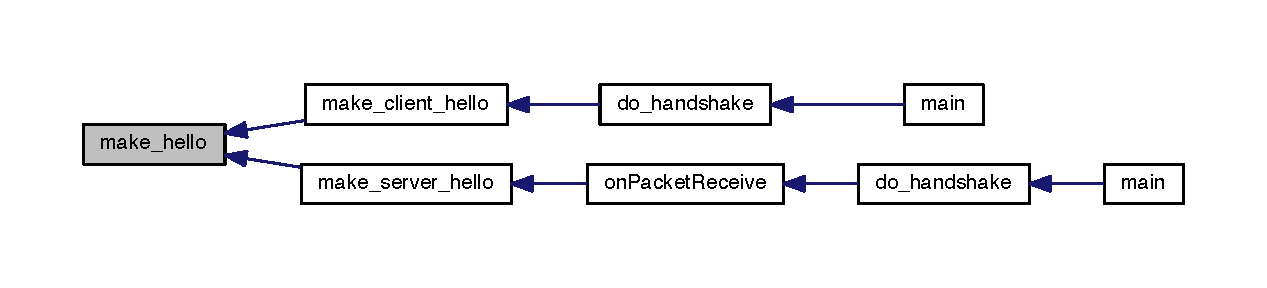
\includegraphics[width=350pt]{_server_client_hello_8h_a095e7c0597d66b5e4eb2097b8f28474a_icgraph}
\end{center}
\end{figure}


\index{Server\+Client\+Hello.\+h@{Server\+Client\+Hello.\+h}!print\+\_\+hello@{print\+\_\+hello}}
\index{print\+\_\+hello@{print\+\_\+hello}!Server\+Client\+Hello.\+h@{Server\+Client\+Hello.\+h}}
\subsubsection[{\texorpdfstring{print\+\_\+hello(server\+\_\+client\+\_\+hello\+\_\+t $\ast$h)}{print_hello(server_client_hello_t *h)}}]{\setlength{\rightskip}{0pt plus 5cm}void print\+\_\+hello (
\begin{DoxyParamCaption}
\item[{{\bf server\+\_\+client\+\_\+hello\+\_\+t} $\ast$}]{h}
\end{DoxyParamCaption}
)}\hypertarget{_server_client_hello_8h_aff8bed251595f5c51c0d1755799909ae}{}\label{_server_client_hello_8h_aff8bed251595f5c51c0d1755799909ae}


Referenced by print\+\_\+handshake().



Here is the caller graph for this function\+:\nopagebreak
\begin{figure}[H]
\begin{center}
\leavevmode
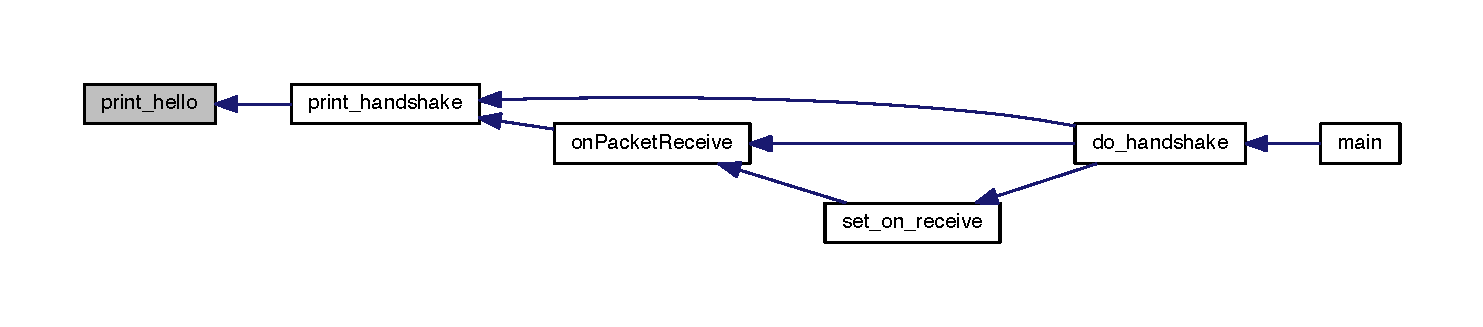
\includegraphics[width=350pt]{_server_client_hello_8h_aff8bed251595f5c51c0d1755799909ae_icgraph}
\end{center}
\end{figure}


\index{Server\+Client\+Hello.\+h@{Server\+Client\+Hello.\+h}!serialize\+\_\+client\+\_\+server\+\_\+hello@{serialize\+\_\+client\+\_\+server\+\_\+hello}}
\index{serialize\+\_\+client\+\_\+server\+\_\+hello@{serialize\+\_\+client\+\_\+server\+\_\+hello}!Server\+Client\+Hello.\+h@{Server\+Client\+Hello.\+h}}
\subsubsection[{\texorpdfstring{serialize\+\_\+client\+\_\+server\+\_\+hello(server\+\_\+client\+\_\+hello\+\_\+t $\ast$hello, unsigned char $\ast$$\ast$stream, uint32\+\_\+t $\ast$stream\+Len, channel\+\_\+mode mode)}{serialize_client_server_hello(server_client_hello_t *hello, unsigned char **stream, uint32_t *streamLen, channel_mode mode)}}]{\setlength{\rightskip}{0pt plus 5cm}void serialize\+\_\+client\+\_\+server\+\_\+hello (
\begin{DoxyParamCaption}
\item[{{\bf server\+\_\+client\+\_\+hello\+\_\+t} $\ast$}]{hello, }
\item[{unsigned char $\ast$$\ast$}]{stream, }
\item[{uint32\+\_\+t $\ast$}]{stream\+Len, }
\item[{{\bf channel\+\_\+mode}}]{mode}
\end{DoxyParamCaption}
)}\hypertarget{_server_client_hello_8h_a5d76fe55dc16550edc3604fcde33b8d0}{}\label{_server_client_hello_8h_a5d76fe55dc16550edc3604fcde33b8d0}


Referenced by make\+\_\+client\+\_\+hello(), and make\+\_\+server\+\_\+hello().



Here is the caller graph for this function\+:\nopagebreak
\begin{figure}[H]
\begin{center}
\leavevmode
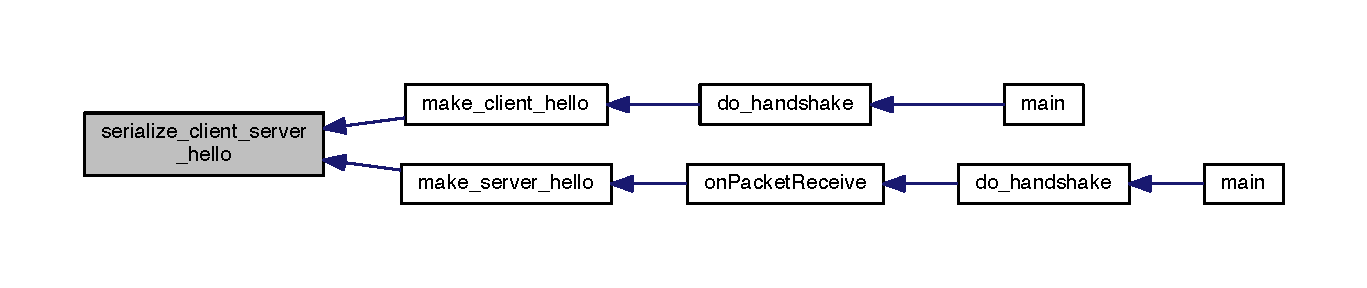
\includegraphics[width=350pt]{_server_client_hello_8h_a5d76fe55dc16550edc3604fcde33b8d0_icgraph}
\end{center}
\end{figure}



\section{/\+Users/\+Darka/\+Dropbox/\+U\+N\+I\+T\+N/\+Advanced\+Programming/\+Project/include/\+Handshake\+Messages/\+Server\+Client\+Key\+Exchange.h File Reference}
\label{_server_client_key_exchange_8h}\index{/\+Users/\+Darka/\+Dropbox/\+U\+N\+I\+T\+N/\+Advanced\+Programming/\+Project/include/\+Handshake\+Messages/\+Server\+Client\+Key\+Exchange.\+h@{/\+Users/\+Darka/\+Dropbox/\+U\+N\+I\+T\+N/\+Advanced\+Programming/\+Project/include/\+Handshake\+Messages/\+Server\+Client\+Key\+Exchange.\+h}}
{\ttfamily \#include $<$stdio.\+h$>$}\\*
{\ttfamily \#include $<$stdlib.\+h$>$}\\*
{\ttfamily \#include $<$string.\+h$>$}\\*
{\ttfamily \#include $<$openssl/hmac.\+h$>$}\\*
{\ttfamily \#include \char`\"{}handshake\+Constants.\+h\char`\"{}}\\*
Include dependency graph for Server\+Client\+Key\+Exchange.\+h\+:\nopagebreak
\begin{figure}[H]
\begin{center}
\leavevmode
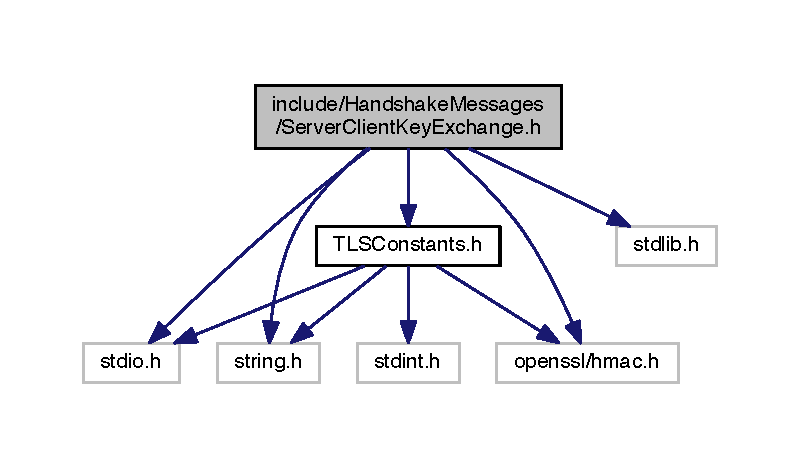
\includegraphics[width=350pt]{_server_client_key_exchange_8h__incl}
\end{center}
\end{figure}
This graph shows which files directly or indirectly include this file\+:\nopagebreak
\begin{figure}[H]
\begin{center}
\leavevmode
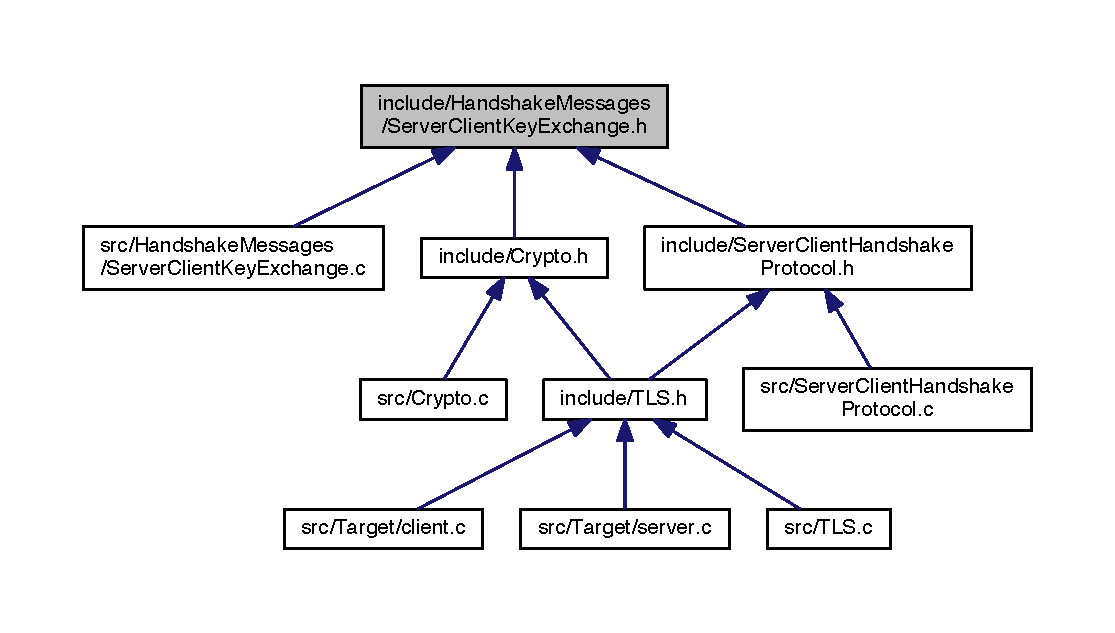
\includegraphics[width=350pt]{_server_client_key_exchange_8h__dep__incl}
\end{center}
\end{figure}
\subsection*{Data Structures}
\begin{DoxyCompactItemize}
\item 
struct {\bf E\+C\+D\+H\+E\+\_\+server\+\_\+key\+\_\+exchange}
\item 
struct {\bf D\+H\+E\+\_\+server\+\_\+key\+\_\+exchange}
\item 
struct {\bf client\+\_\+key\+\_\+exchange}
\end{DoxyCompactItemize}
\subsection*{Macros}
\begin{DoxyCompactItemize}
\item 
\#define {\bf server\+\_\+key\+\_\+exchange\+\_\+structs}
\end{DoxyCompactItemize}
\subsection*{Functions}
\begin{DoxyCompactItemize}
\item 
void {\bf serialize\+\_\+server\+\_\+key\+\_\+exchange} (void $\ast$server\+\_\+key\+\_\+exchange, unsigned char $\ast$$\ast$stream, uint32\+\_\+t $\ast$stream\+Len, {\bf key\+\_\+exchange\+\_\+algorithm} kx)
\item 
void $\ast$ {\bf deserialize\+\_\+server\+\_\+key\+\_\+exchange} (uint32\+\_\+t message\+\_\+len, unsigned char $\ast$message, {\bf key\+\_\+exchange\+\_\+algorithm} kx)
\item 
void {\bf serialize\+\_\+client\+\_\+key\+\_\+exchange} ({\bf client\+\_\+key\+\_\+exchange} $\ast${\bf client\+\_\+key\+\_\+exchange}, unsigned char $\ast$$\ast$stream, uint32\+\_\+t $\ast$stream\+Len)
\item 
void $\ast$ {\bf deserialize\+\_\+client\+\_\+key\+\_\+exchange} (uint32\+\_\+t message\+\_\+len, unsigned char $\ast$message)
\item 
void {\bf free\+\_\+server\+\_\+key\+\_\+exchange} (void $\ast$server\+\_\+key\+\_\+ex, {\bf cipher\+\_\+suite\+\_\+t} cipher\+\_\+suite)
\end{DoxyCompactItemize}


\subsection{Macro Definition Documentation}
\index{Server\+Client\+Key\+Exchange.\+h@{Server\+Client\+Key\+Exchange.\+h}!server\+\_\+key\+\_\+exchange\+\_\+structs@{server\+\_\+key\+\_\+exchange\+\_\+structs}}
\index{server\+\_\+key\+\_\+exchange\+\_\+structs@{server\+\_\+key\+\_\+exchange\+\_\+structs}!Server\+Client\+Key\+Exchange.\+h@{Server\+Client\+Key\+Exchange.\+h}}
\subsubsection[{server\+\_\+key\+\_\+exchange\+\_\+structs}]{\setlength{\rightskip}{0pt plus 5cm}\#define server\+\_\+key\+\_\+exchange\+\_\+structs}\label{_server_client_key_exchange_8h_a996cafa3e26488efea4ff4ad13c6a32f}


Definition at line 24 of file Server\+Client\+Key\+Exchange.\+h.



\subsection{Function Documentation}
\index{Server\+Client\+Key\+Exchange.\+h@{Server\+Client\+Key\+Exchange.\+h}!deserialize\+\_\+client\+\_\+key\+\_\+exchange@{deserialize\+\_\+client\+\_\+key\+\_\+exchange}}
\index{deserialize\+\_\+client\+\_\+key\+\_\+exchange@{deserialize\+\_\+client\+\_\+key\+\_\+exchange}!Server\+Client\+Key\+Exchange.\+h@{Server\+Client\+Key\+Exchange.\+h}}
\subsubsection[{deserialize\+\_\+client\+\_\+key\+\_\+exchange(uint32\+\_\+t message\+\_\+len, unsigned char $\ast$message)}]{\setlength{\rightskip}{0pt plus 5cm}void$\ast$ deserialize\+\_\+client\+\_\+key\+\_\+exchange (
\begin{DoxyParamCaption}
\item[{uint32\+\_\+t}]{message\+\_\+len, }
\item[{unsigned char $\ast$}]{message}
\end{DoxyParamCaption}
)}\label{_server_client_key_exchange_8h_a225e72dcfe80ab6f0bd08043a3c264a0}


Definition at line 185 of file Server\+Client\+Key\+Exchange.\+c.



Here is the caller graph for this function\+:\nopagebreak
\begin{figure}[H]
\begin{center}
\leavevmode
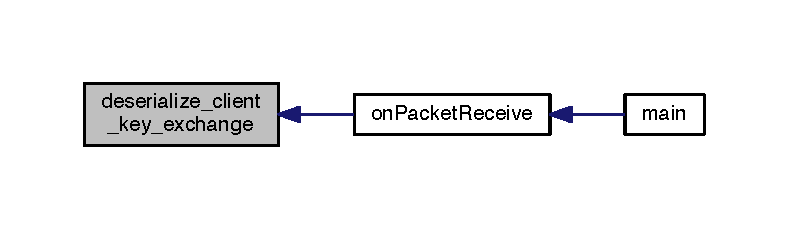
\includegraphics[width=350pt]{_server_client_key_exchange_8h_a225e72dcfe80ab6f0bd08043a3c264a0_icgraph}
\end{center}
\end{figure}


\index{Server\+Client\+Key\+Exchange.\+h@{Server\+Client\+Key\+Exchange.\+h}!deserialize\+\_\+server\+\_\+key\+\_\+exchange@{deserialize\+\_\+server\+\_\+key\+\_\+exchange}}
\index{deserialize\+\_\+server\+\_\+key\+\_\+exchange@{deserialize\+\_\+server\+\_\+key\+\_\+exchange}!Server\+Client\+Key\+Exchange.\+h@{Server\+Client\+Key\+Exchange.\+h}}
\subsubsection[{deserialize\+\_\+server\+\_\+key\+\_\+exchange(uint32\+\_\+t message\+\_\+len, unsigned char $\ast$message, key\+\_\+exchange\+\_\+algorithm kx)}]{\setlength{\rightskip}{0pt plus 5cm}void$\ast$ deserialize\+\_\+server\+\_\+key\+\_\+exchange (
\begin{DoxyParamCaption}
\item[{uint32\+\_\+t}]{message\+\_\+len, }
\item[{unsigned char $\ast$}]{message, }
\item[{{\bf key\+\_\+exchange\+\_\+algorithm}}]{kx}
\end{DoxyParamCaption}
)}\label{_server_client_key_exchange_8h_a8eb5113e9d14196b6c1dbe3df1c56c06}


Definition at line 104 of file Server\+Client\+Key\+Exchange.\+c.



Here is the caller graph for this function\+:\nopagebreak
\begin{figure}[H]
\begin{center}
\leavevmode
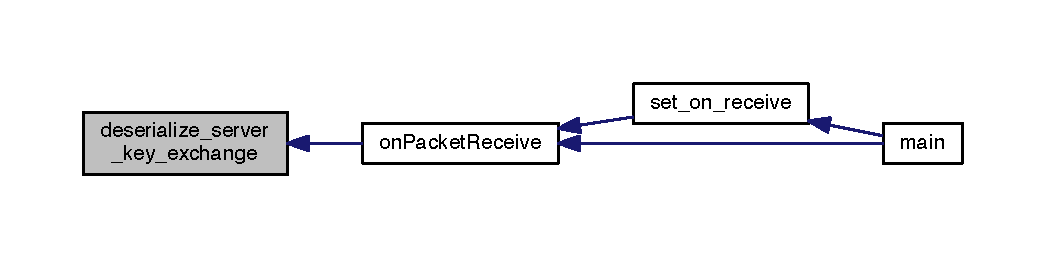
\includegraphics[width=350pt]{_server_client_key_exchange_8h_a8eb5113e9d14196b6c1dbe3df1c56c06_icgraph}
\end{center}
\end{figure}


\index{Server\+Client\+Key\+Exchange.\+h@{Server\+Client\+Key\+Exchange.\+h}!free\+\_\+server\+\_\+key\+\_\+exchange@{free\+\_\+server\+\_\+key\+\_\+exchange}}
\index{free\+\_\+server\+\_\+key\+\_\+exchange@{free\+\_\+server\+\_\+key\+\_\+exchange}!Server\+Client\+Key\+Exchange.\+h@{Server\+Client\+Key\+Exchange.\+h}}
\subsubsection[{free\+\_\+server\+\_\+key\+\_\+exchange(void $\ast$server\+\_\+key\+\_\+ex, cipher\+\_\+suite\+\_\+t cipher\+\_\+suite)}]{\setlength{\rightskip}{0pt plus 5cm}void free\+\_\+server\+\_\+key\+\_\+exchange (
\begin{DoxyParamCaption}
\item[{void $\ast$}]{server\+\_\+key\+\_\+ex, }
\item[{{\bf cipher\+\_\+suite\+\_\+t}}]{cipher\+\_\+suite}
\end{DoxyParamCaption}
)}\label{_server_client_key_exchange_8h_a9b34f5779b31eb5a18a2fc5c644aaa78}


Definition at line 199 of file Server\+Client\+Key\+Exchange.\+c.



Here is the caller graph for this function\+:\nopagebreak
\begin{figure}[H]
\begin{center}
\leavevmode
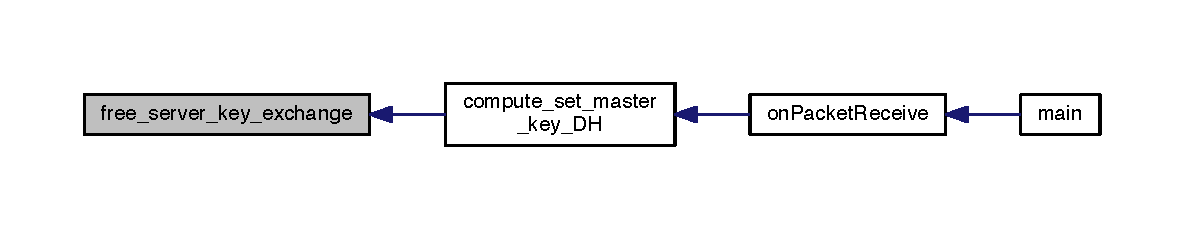
\includegraphics[width=350pt]{_server_client_key_exchange_8h_a9b34f5779b31eb5a18a2fc5c644aaa78_icgraph}
\end{center}
\end{figure}


\index{Server\+Client\+Key\+Exchange.\+h@{Server\+Client\+Key\+Exchange.\+h}!serialize\+\_\+client\+\_\+key\+\_\+exchange@{serialize\+\_\+client\+\_\+key\+\_\+exchange}}
\index{serialize\+\_\+client\+\_\+key\+\_\+exchange@{serialize\+\_\+client\+\_\+key\+\_\+exchange}!Server\+Client\+Key\+Exchange.\+h@{Server\+Client\+Key\+Exchange.\+h}}
\subsubsection[{serialize\+\_\+client\+\_\+key\+\_\+exchange(client\+\_\+key\+\_\+exchange $\ast$client\+\_\+key\+\_\+exchange, unsigned char $\ast$$\ast$stream, uint32\+\_\+t $\ast$stream\+Len)}]{\setlength{\rightskip}{0pt plus 5cm}void serialize\+\_\+client\+\_\+key\+\_\+exchange (
\begin{DoxyParamCaption}
\item[{{\bf client\+\_\+key\+\_\+exchange} $\ast$}]{client\+\_\+key\+\_\+exchange, }
\item[{unsigned char $\ast$$\ast$}]{stream, }
\item[{uint32\+\_\+t $\ast$}]{stream\+Len}
\end{DoxyParamCaption}
)}\label{_server_client_key_exchange_8h_a0c677b3ebb47b3db1a455bc051384af9}


Definition at line 171 of file Server\+Client\+Key\+Exchange.\+c.



Here is the caller graph for this function\+:\nopagebreak
\begin{figure}[H]
\begin{center}
\leavevmode
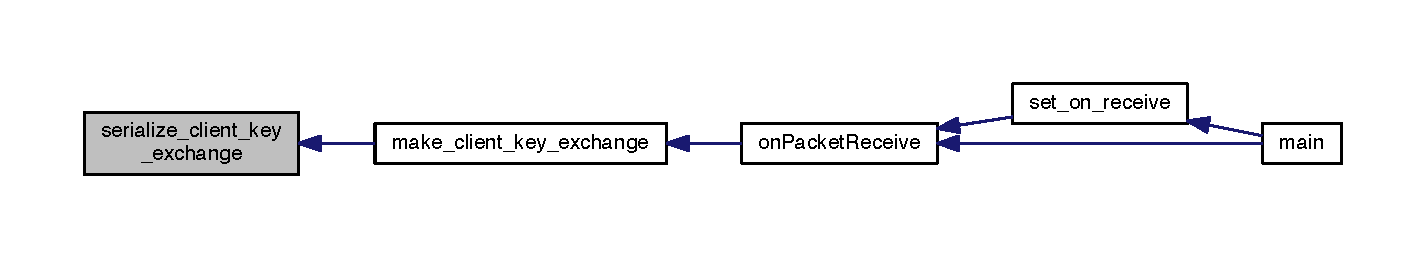
\includegraphics[width=350pt]{_server_client_key_exchange_8h_a0c677b3ebb47b3db1a455bc051384af9_icgraph}
\end{center}
\end{figure}


\index{Server\+Client\+Key\+Exchange.\+h@{Server\+Client\+Key\+Exchange.\+h}!serialize\+\_\+server\+\_\+key\+\_\+exchange@{serialize\+\_\+server\+\_\+key\+\_\+exchange}}
\index{serialize\+\_\+server\+\_\+key\+\_\+exchange@{serialize\+\_\+server\+\_\+key\+\_\+exchange}!Server\+Client\+Key\+Exchange.\+h@{Server\+Client\+Key\+Exchange.\+h}}
\subsubsection[{serialize\+\_\+server\+\_\+key\+\_\+exchange(void $\ast$server\+\_\+key\+\_\+exchange, unsigned char $\ast$$\ast$stream, uint32\+\_\+t $\ast$stream\+Len, key\+\_\+exchange\+\_\+algorithm kx)}]{\setlength{\rightskip}{0pt plus 5cm}void serialize\+\_\+server\+\_\+key\+\_\+exchange (
\begin{DoxyParamCaption}
\item[{void $\ast$}]{server\+\_\+key\+\_\+exchange, }
\item[{unsigned char $\ast$$\ast$}]{stream, }
\item[{uint32\+\_\+t $\ast$}]{stream\+Len, }
\item[{{\bf key\+\_\+exchange\+\_\+algorithm}}]{kx}
\end{DoxyParamCaption}
)}\label{_server_client_key_exchange_8h_a290e31280396f330234592d27ac3b2d9}


Definition at line 15 of file Server\+Client\+Key\+Exchange.\+c.



Here is the caller graph for this function\+:\nopagebreak
\begin{figure}[H]
\begin{center}
\leavevmode
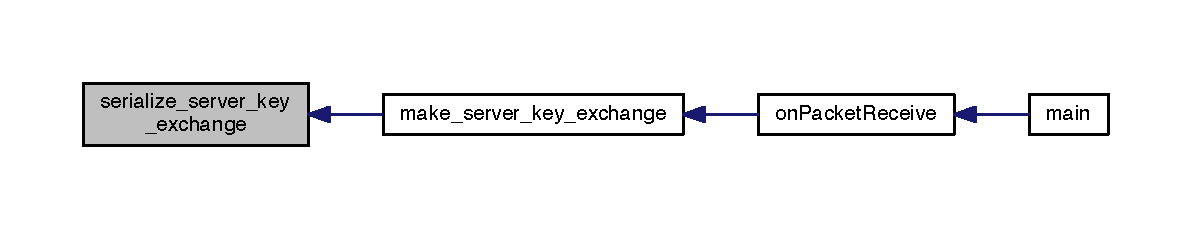
\includegraphics[width=350pt]{_server_client_key_exchange_8h_a290e31280396f330234592d27ac3b2d9_icgraph}
\end{center}
\end{figure}



\hypertarget{_server_client_handshake_protocol_8h}{}\section{/\+Users/\+Darka/\+Dropbox/\+U\+N\+I\+T\+N/\+Advanced\+Programming/\+Project/include/\+Server\+Client\+Handshake\+Protocol.h File Reference}
\label{_server_client_handshake_protocol_8h}\index{/\+Users/\+Darka/\+Dropbox/\+U\+N\+I\+T\+N/\+Advanced\+Programming/\+Project/include/\+Server\+Client\+Handshake\+Protocol.\+h@{/\+Users/\+Darka/\+Dropbox/\+U\+N\+I\+T\+N/\+Advanced\+Programming/\+Project/include/\+Server\+Client\+Handshake\+Protocol.\+h}}
{\ttfamily \#include $<$stdio.\+h$>$}\\*
{\ttfamily \#include $<$stdint.\+h$>$}\\*
{\ttfamily \#include $<$time.\+h$>$}\\*
{\ttfamily \#include $<$stdlib.\+h$>$}\\*
{\ttfamily \#include $<$string.\+h$>$}\\*
{\ttfamily \#include \char`\"{}Server\+Client\+Record\+Protocol.\+h\char`\"{}}\\*
{\ttfamily \#include \char`\"{}T\+L\+S\+Constants.\+h\char`\"{}}\\*
{\ttfamily \#include \char`\"{}Server\+Client\+Hello.\+h\char`\"{}}\\*
{\ttfamily \#include \char`\"{}Certificate.\+h\char`\"{}}\\*
{\ttfamily \#include \char`\"{}Server\+Client\+Key\+Exchange.\+h\char`\"{}}\\*
\subsection*{Data Structures}
\begin{DoxyCompactItemize}
\item 
struct \hyperlink{structhandshake__t}{handshake\+\_\+t}
\end{DoxyCompactItemize}
\subsection*{Functions}
\begin{DoxyCompactItemize}
\item 
int \hyperlink{_server_client_handshake_protocol_8h_a630be726ff62f89c4287fa0feb6e3801}{send\+\_\+handshake} (\hyperlink{structchannel__t}{channel\+\_\+t} $\ast$ch, \hyperlink{structhandshake__t}{handshake\+\_\+t} $\ast$h)
\item 
void \hyperlink{_server_client_handshake_protocol_8h_a1f9226db59b1fe4f860122d082429f78}{serialize\+\_\+handshake} (\hyperlink{structhandshake__t}{handshake\+\_\+t} $\ast$h, unsigned char $\ast$$\ast$stream, uint32\+\_\+t $\ast$stream\+Len)
\item 
\hyperlink{structhandshake__t}{handshake\+\_\+t} $\ast$ \hyperlink{_server_client_handshake_protocol_8h_a9f902224a1dcf6201a60941914a0fb2d}{deserialize\+\_\+handshake} (unsigned char $\ast$message, uint32\+\_\+t message\+Len)
\item 
void \hyperlink{_server_client_handshake_protocol_8h_a17a2f489bf364bdd80fbd20d186f927e}{print\+\_\+handshake} (\hyperlink{structhandshake__t}{handshake\+\_\+t} $\ast$h, int verbosity, \hyperlink{_t_l_s_constants_8h_a7203e83530e35d8ed2f3300ba0408a54}{key\+\_\+exchange\+\_\+algorithm} kx)
\item 
void \hyperlink{_server_client_handshake_protocol_8h_a5b7a13680988ecee1fd6c0a8dfe32eef}{free\+\_\+handshake} (\hyperlink{structhandshake__t}{handshake\+\_\+t} $\ast$h)
\end{DoxyCompactItemize}


\subsection{Detailed Description}
S\+S\+L/\+T\+LS Project

This file is used to mange the handshake protocol

\begin{DoxyDate}{Date}
Created on 27/12/15. 
\end{DoxyDate}
\begin{DoxyCopyright}{Copyright}
Copyright © 2015 Alessandro Melloni, Andrea Francesco Vinci. All rights reserved. 
\end{DoxyCopyright}


\subsection{Function Documentation}
\index{Server\+Client\+Handshake\+Protocol.\+h@{Server\+Client\+Handshake\+Protocol.\+h}!deserialize\+\_\+handshake@{deserialize\+\_\+handshake}}
\index{deserialize\+\_\+handshake@{deserialize\+\_\+handshake}!Server\+Client\+Handshake\+Protocol.\+h@{Server\+Client\+Handshake\+Protocol.\+h}}
\subsubsection[{\texorpdfstring{deserialize\+\_\+handshake(unsigned char $\ast$message, uint32\+\_\+t message\+Len)}{deserialize_handshake(unsigned char *message, uint32_t messageLen)}}]{\setlength{\rightskip}{0pt plus 5cm}{\bf handshake\+\_\+t}$\ast$ deserialize\+\_\+handshake (
\begin{DoxyParamCaption}
\item[{unsigned char $\ast$}]{message, }
\item[{uint32\+\_\+t}]{message\+Len}
\end{DoxyParamCaption}
)}\hypertarget{_server_client_handshake_protocol_8h_a9f902224a1dcf6201a60941914a0fb2d}{}\label{_server_client_handshake_protocol_8h_a9f902224a1dcf6201a60941914a0fb2d}
De-\/serialize a stream of byte into an handshake.


\begin{DoxyParams}{Parameters}
{\em message} & \+: the serialized handshake \\
\hline
{\em message\+Len} & \+: the message length \\
\hline
\end{DoxyParams}
\begin{DoxyReturn}{Returns}
alloc and return an handshake struct 
\end{DoxyReturn}


Referenced by on\+Packet\+Receive().

\index{Server\+Client\+Handshake\+Protocol.\+h@{Server\+Client\+Handshake\+Protocol.\+h}!free\+\_\+handshake@{free\+\_\+handshake}}
\index{free\+\_\+handshake@{free\+\_\+handshake}!Server\+Client\+Handshake\+Protocol.\+h@{Server\+Client\+Handshake\+Protocol.\+h}}
\subsubsection[{\texorpdfstring{free\+\_\+handshake(handshake\+\_\+t $\ast$h)}{free_handshake(handshake_t *h)}}]{\setlength{\rightskip}{0pt plus 5cm}void free\+\_\+handshake (
\begin{DoxyParamCaption}
\item[{{\bf handshake\+\_\+t} $\ast$}]{h}
\end{DoxyParamCaption}
)}\hypertarget{_server_client_handshake_protocol_8h_a5b7a13680988ecee1fd6c0a8dfe32eef}{}\label{_server_client_handshake_protocol_8h_a5b7a13680988ecee1fd6c0a8dfe32eef}
Delloc memory of handshake struct


\begin{DoxyParams}{Parameters}
{\em h} & \+: the handshake to free \\
\hline
\end{DoxyParams}


Referenced by do\+\_\+handshake(), and on\+Packet\+Receive().

\index{Server\+Client\+Handshake\+Protocol.\+h@{Server\+Client\+Handshake\+Protocol.\+h}!print\+\_\+handshake@{print\+\_\+handshake}}
\index{print\+\_\+handshake@{print\+\_\+handshake}!Server\+Client\+Handshake\+Protocol.\+h@{Server\+Client\+Handshake\+Protocol.\+h}}
\subsubsection[{\texorpdfstring{print\+\_\+handshake(handshake\+\_\+t $\ast$h, int verbosity, key\+\_\+exchange\+\_\+algorithm kx)}{print_handshake(handshake_t *h, int verbosity, key_exchange_algorithm kx)}}]{\setlength{\rightskip}{0pt plus 5cm}void print\+\_\+handshake (
\begin{DoxyParamCaption}
\item[{{\bf handshake\+\_\+t} $\ast$}]{h, }
\item[{int}]{verbosity, }
\item[{{\bf key\+\_\+exchange\+\_\+algorithm}}]{kx}
\end{DoxyParamCaption}
)}\hypertarget{_server_client_handshake_protocol_8h_a17a2f489bf364bdd80fbd20d186f927e}{}\label{_server_client_handshake_protocol_8h_a17a2f489bf364bdd80fbd20d186f927e}
Print an handshake struct


\begin{DoxyParams}{Parameters}
{\em h} & \+: handshake to print \\
\hline
{\em verobisty} & \+: how many detail to print (0 none, 1 the binary, 2 details) \\
\hline
{\em kx} & \+: the key exchange algorithm, useful in key\+\_\+echange messages \\
\hline
\end{DoxyParams}


Referenced by do\+\_\+handshake(), and on\+Packet\+Receive().

\index{Server\+Client\+Handshake\+Protocol.\+h@{Server\+Client\+Handshake\+Protocol.\+h}!send\+\_\+handshake@{send\+\_\+handshake}}
\index{send\+\_\+handshake@{send\+\_\+handshake}!Server\+Client\+Handshake\+Protocol.\+h@{Server\+Client\+Handshake\+Protocol.\+h}}
\subsubsection[{\texorpdfstring{send\+\_\+handshake(channel\+\_\+t $\ast$ch, handshake\+\_\+t $\ast$h)}{send_handshake(channel_t *ch, handshake_t *h)}}]{\setlength{\rightskip}{0pt plus 5cm}int send\+\_\+handshake (
\begin{DoxyParamCaption}
\item[{{\bf channel\+\_\+t} $\ast$}]{ch, }
\item[{{\bf handshake\+\_\+t} $\ast$}]{h}
\end{DoxyParamCaption}
)}\hypertarget{_server_client_handshake_protocol_8h_a630be726ff62f89c4287fa0feb6e3801}{}\label{_server_client_handshake_protocol_8h_a630be726ff62f89c4287fa0feb6e3801}
Send an handshake through a channel


\begin{DoxyParams}{Parameters}
{\em ch} & \+: the channel to use \\
\hline
{\em h} & \+: the handshake to send \\
\hline
\end{DoxyParams}
\begin{DoxyReturn}{Returns}
1 if the send is success, 0 otherwise 
\end{DoxyReturn}


Referenced by do\+\_\+handshake(), and on\+Packet\+Receive().

\index{Server\+Client\+Handshake\+Protocol.\+h@{Server\+Client\+Handshake\+Protocol.\+h}!serialize\+\_\+handshake@{serialize\+\_\+handshake}}
\index{serialize\+\_\+handshake@{serialize\+\_\+handshake}!Server\+Client\+Handshake\+Protocol.\+h@{Server\+Client\+Handshake\+Protocol.\+h}}
\subsubsection[{\texorpdfstring{serialize\+\_\+handshake(handshake\+\_\+t $\ast$h, unsigned char $\ast$$\ast$stream, uint32\+\_\+t $\ast$stream\+Len)}{serialize_handshake(handshake_t *h, unsigned char **stream, uint32_t *streamLen)}}]{\setlength{\rightskip}{0pt plus 5cm}void serialize\+\_\+handshake (
\begin{DoxyParamCaption}
\item[{{\bf handshake\+\_\+t} $\ast$}]{h, }
\item[{unsigned char $\ast$$\ast$}]{stream, }
\item[{uint32\+\_\+t $\ast$}]{stream\+Len}
\end{DoxyParamCaption}
)}\hypertarget{_server_client_handshake_protocol_8h_a1f9226db59b1fe4f860122d082429f78}{}\label{_server_client_handshake_protocol_8h_a1f9226db59b1fe4f860122d082429f78}
Serialize a handshake into a byte stream


\begin{DoxyParams}{Parameters}
{\em h} & \+: the handshake to serialize \\
\hline
{\em stream} & \+: a pointer to N\+U\+LL, it will filled with the serialized handshake \\
\hline
{\em stream\+Len} & \+: the length of the serialized message \\
\hline
\end{DoxyParams}


Referenced by backup\+\_\+handshake(), make\+\_\+record(), and print\+\_\+handshake().


\hypertarget{_server_client_record_protocol_8h}{}\section{include/\+Server\+Client\+Record\+Protocol.h File Reference}
\label{_server_client_record_protocol_8h}\index{include/\+Server\+Client\+Record\+Protocol.\+h@{include/\+Server\+Client\+Record\+Protocol.\+h}}
{\ttfamily \#include $<$stdio.\+h$>$}\\*
{\ttfamily \#include \char`\"{}Server\+Client\+Transport\+Protocol.\+h\char`\"{}}\\*
Include dependency graph for Server\+Client\+Record\+Protocol.\+h\+:
\nopagebreak
\begin{figure}[H]
\begin{center}
\leavevmode
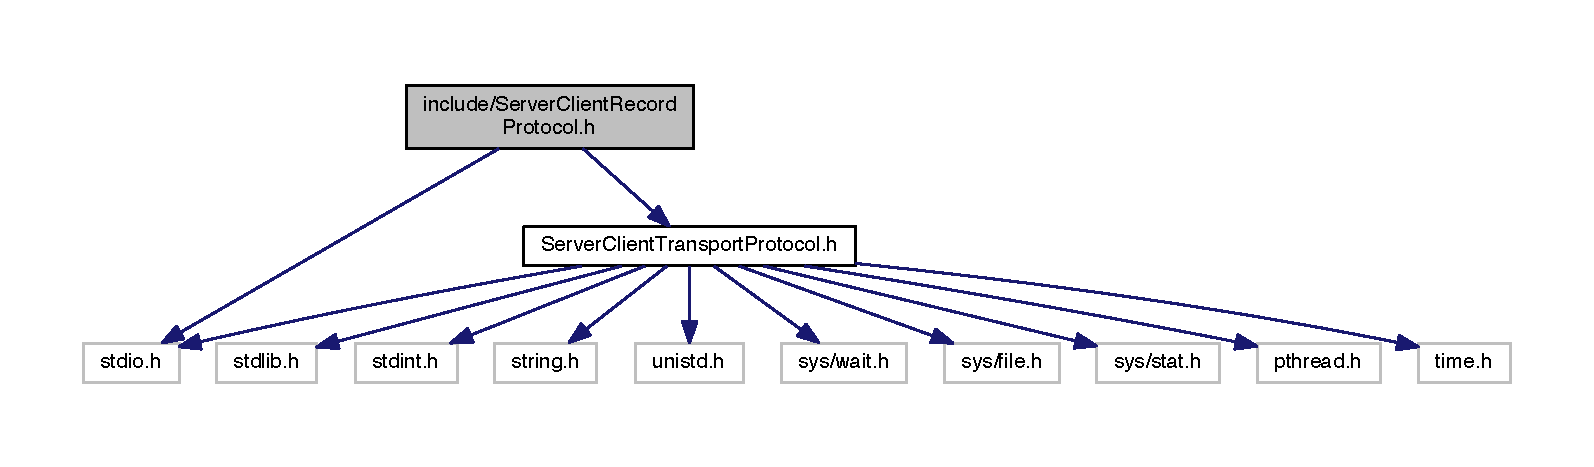
\includegraphics[width=350pt]{_server_client_record_protocol_8h__incl}
\end{center}
\end{figure}
This graph shows which files directly or indirectly include this file\+:
\nopagebreak
\begin{figure}[H]
\begin{center}
\leavevmode
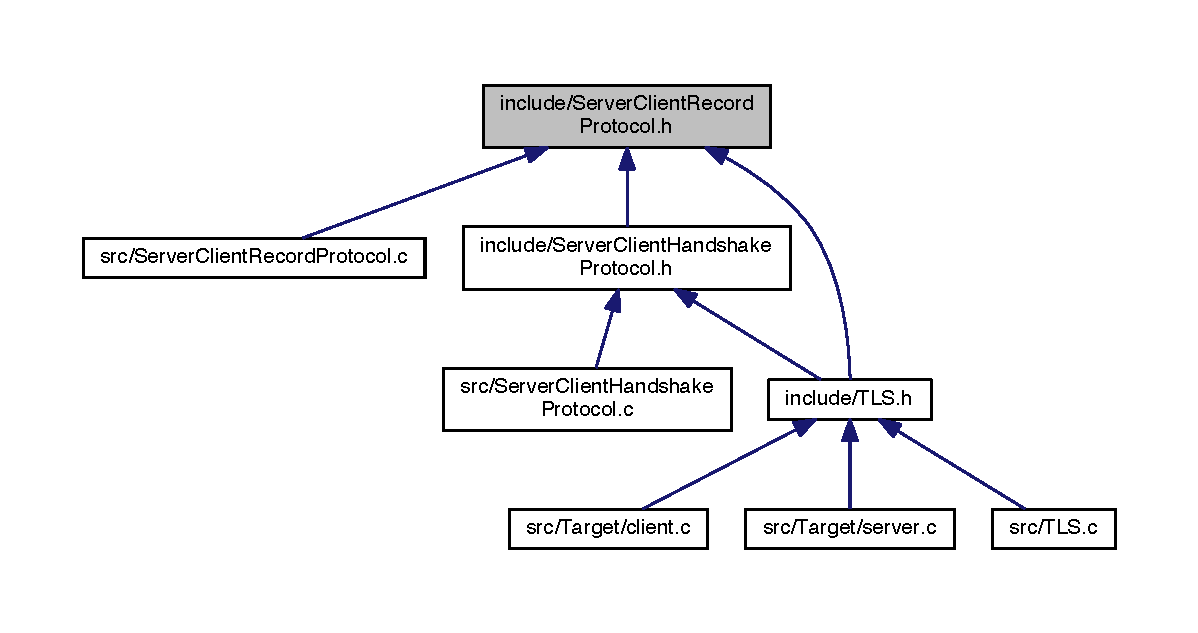
\includegraphics[width=350pt]{_server_client_record_protocol_8h__dep__incl}
\end{center}
\end{figure}
\subsection*{Data Structures}
\begin{DoxyCompactItemize}
\item 
struct \hyperlink{structrecord__t}{record\+\_\+t}
\end{DoxyCompactItemize}
\subsection*{Macros}
\begin{DoxyCompactItemize}
\item 
\#define \hyperlink{_server_client_record_protocol_8h_ab7690321561c4c2f8e301abd41440aa4}{R\+E\+V16}(value)~(\{(value \& 0x00\+F\+F\+U) $<$$<$ 8 $\vert$ (value \& 0x\+F\+F00\+U) $>$$>$ 8;\})
\end{DoxyCompactItemize}
\subsection*{Enumerations}
\subsection*{Functions}
\begin{DoxyCompactItemize}
\item 
int \hyperlink{_server_client_record_protocol_8h_a1ceb817bc488ec68b8abfd289dbbf6c0}{send\+\_\+record} (\hyperlink{structchannel__t}{channel\+\_\+t} $\ast$ch, \hyperlink{structrecord__t}{record\+\_\+t} $\ast$to\+\_\+send)
\item 
\hyperlink{structrecord__t}{record\+\_\+t} $\ast$ \hyperlink{_server_client_record_protocol_8h_abb4c45954ce00d016a651588a179ff19}{deserialize\+\_\+record} (unsigned char $\ast$message, uint32\+\_\+t message\+\_\+len)
\item 
void \hyperlink{_server_client_record_protocol_8h_af6de1ff6a0b52cc2ad9224dbc4e9a14c}{serialize\+\_\+record} (\hyperlink{structrecord__t}{record\+\_\+t} $\ast$r, unsigned char $\ast$$\ast$message, uint16\+\_\+t $\ast$message\+\_\+len)
\item 
void \hyperlink{_server_client_record_protocol_8h_a5029bcdf9f7eb874b25136b76e41963c}{print\+\_\+record} (\hyperlink{structrecord__t}{record\+\_\+t} $\ast$r)
\item 
void \hyperlink{_server_client_record_protocol_8h_a9212df7db09a62df2f7d4a913f04defc}{free\+\_\+record} (\hyperlink{structrecord__t}{record\+\_\+t} $\ast$r)
\end{DoxyCompactItemize}


\subsection{Detailed Description}
S\+S\+L/\+T\+LS Project

This file is an interface to the record protocol. Provide function and struct for modelling and manage record messages.

\begin{DoxyDate}{Date}
Created on 23/12/15. 
\end{DoxyDate}
\begin{DoxyCopyright}{Copyright}
Copyright © 2015 Alessandro Melloni, Andrea Francesco Vinci. All rights reserved. 
\end{DoxyCopyright}


\subsection{Macro Definition Documentation}
\index{Server\+Client\+Record\+Protocol.\+h@{Server\+Client\+Record\+Protocol.\+h}!R\+E\+V16@{R\+E\+V16}}
\index{R\+E\+V16@{R\+E\+V16}!Server\+Client\+Record\+Protocol.\+h@{Server\+Client\+Record\+Protocol.\+h}}
\subsubsection[{\texorpdfstring{R\+E\+V16}{REV16}}]{\setlength{\rightskip}{0pt plus 5cm}\#define R\+E\+V16(
\begin{DoxyParamCaption}
\item[{}]{value}
\end{DoxyParamCaption}
)~(\{(value \& 0x00\+F\+F\+U) $<$$<$ 8 $\vert$ (value \& 0x\+F\+F00\+U) $>$$>$ 8;\})}\hypertarget{_server_client_record_protocol_8h_ab7690321561c4c2f8e301abd41440aa4}{}\label{_server_client_record_protocol_8h_ab7690321561c4c2f8e301abd41440aa4}
Rotational byte for uint16 

Referenced by deserialize\+\_\+client\+\_\+key\+\_\+exchange(), deserialize\+\_\+client\+\_\+server\+\_\+hello(), deserialize\+\_\+record(), deserialize\+\_\+server\+\_\+key\+\_\+exchange(), make\+\_\+\+R\+S\+A\+\_\+client\+\_\+key\+\_\+exchange(), serialize\+\_\+client\+\_\+key\+\_\+exchange(), serialize\+\_\+client\+\_\+server\+\_\+hello(), serialize\+\_\+record(), and serialize\+\_\+server\+\_\+key\+\_\+exchange().



\subsection{Enumeration Type Documentation}
\index{Server\+Client\+Record\+Protocol.\+h@{Server\+Client\+Record\+Protocol.\+h}!record\+\_\+type@{record\+\_\+type}}
\index{record\+\_\+type@{record\+\_\+type}!Server\+Client\+Record\+Protocol.\+h@{Server\+Client\+Record\+Protocol.\+h}}
\subsubsection[{\texorpdfstring{record\+\_\+type}{record_type}}]{\setlength{\rightskip}{0pt plus 5cm}enum {\bf record\+\_\+type}}\hypertarget{_server_client_record_protocol_8h_a393986e23103348f07699f24dcb7f238}{}\label{_server_client_record_protocol_8h_a393986e23103348f07699f24dcb7f238}
Define the different type of record \begin{Desc}
\item[Enumerator]\par
\begin{description}
\index{H\+A\+N\+D\+S\+H\+A\+KE@{H\+A\+N\+D\+S\+H\+A\+KE}!Server\+Client\+Record\+Protocol.\+h@{Server\+Client\+Record\+Protocol.\+h}}\index{Server\+Client\+Record\+Protocol.\+h@{Server\+Client\+Record\+Protocol.\+h}!H\+A\+N\+D\+S\+H\+A\+KE@{H\+A\+N\+D\+S\+H\+A\+KE}}\item[{\em 
H\+A\+N\+D\+S\+H\+A\+KE\hypertarget{_server_client_record_protocol_8h_a393986e23103348f07699f24dcb7f238acc6ddcaa36bd57e5aec12749cb5ce29c}{}\label{_server_client_record_protocol_8h_a393986e23103348f07699f24dcb7f238acc6ddcaa36bd57e5aec12749cb5ce29c}
}]\index{C\+H\+A\+N\+G\+E\+\_\+\+C\+I\+P\+H\+E\+R\+\_\+\+S\+P\+EC@{C\+H\+A\+N\+G\+E\+\_\+\+C\+I\+P\+H\+E\+R\+\_\+\+S\+P\+EC}!Server\+Client\+Record\+Protocol.\+h@{Server\+Client\+Record\+Protocol.\+h}}\index{Server\+Client\+Record\+Protocol.\+h@{Server\+Client\+Record\+Protocol.\+h}!C\+H\+A\+N\+G\+E\+\_\+\+C\+I\+P\+H\+E\+R\+\_\+\+S\+P\+EC@{C\+H\+A\+N\+G\+E\+\_\+\+C\+I\+P\+H\+E\+R\+\_\+\+S\+P\+EC}}\item[{\em 
C\+H\+A\+N\+G\+E\+\_\+\+C\+I\+P\+H\+E\+R\+\_\+\+S\+P\+EC\hypertarget{_server_client_record_protocol_8h_a393986e23103348f07699f24dcb7f238a4ba5b5ec083856acccc568fff147a664}{}\label{_server_client_record_protocol_8h_a393986e23103348f07699f24dcb7f238a4ba5b5ec083856acccc568fff147a664}
}]\index{A\+L\+E\+RT@{A\+L\+E\+RT}!Server\+Client\+Record\+Protocol.\+h@{Server\+Client\+Record\+Protocol.\+h}}\index{Server\+Client\+Record\+Protocol.\+h@{Server\+Client\+Record\+Protocol.\+h}!A\+L\+E\+RT@{A\+L\+E\+RT}}\item[{\em 
A\+L\+E\+RT\hypertarget{_server_client_record_protocol_8h_a393986e23103348f07699f24dcb7f238a45e0bb0f520fb3851c7d6cc5c5ddd6f9}{}\label{_server_client_record_protocol_8h_a393986e23103348f07699f24dcb7f238a45e0bb0f520fb3851c7d6cc5c5ddd6f9}
}]\index{A\+P\+P\+L\+I\+C\+A\+T\+I\+O\+N\+\_\+\+D\+A\+TA@{A\+P\+P\+L\+I\+C\+A\+T\+I\+O\+N\+\_\+\+D\+A\+TA}!Server\+Client\+Record\+Protocol.\+h@{Server\+Client\+Record\+Protocol.\+h}}\index{Server\+Client\+Record\+Protocol.\+h@{Server\+Client\+Record\+Protocol.\+h}!A\+P\+P\+L\+I\+C\+A\+T\+I\+O\+N\+\_\+\+D\+A\+TA@{A\+P\+P\+L\+I\+C\+A\+T\+I\+O\+N\+\_\+\+D\+A\+TA}}\item[{\em 
A\+P\+P\+L\+I\+C\+A\+T\+I\+O\+N\+\_\+\+D\+A\+TA\hypertarget{_server_client_record_protocol_8h_a393986e23103348f07699f24dcb7f238ae5600c9ebf3ad742718c2ba003539a45}{}\label{_server_client_record_protocol_8h_a393986e23103348f07699f24dcb7f238ae5600c9ebf3ad742718c2ba003539a45}
}]\end{description}
\end{Desc}


\subsection{Function Documentation}
\index{Server\+Client\+Record\+Protocol.\+h@{Server\+Client\+Record\+Protocol.\+h}!deserialize\+\_\+record@{deserialize\+\_\+record}}
\index{deserialize\+\_\+record@{deserialize\+\_\+record}!Server\+Client\+Record\+Protocol.\+h@{Server\+Client\+Record\+Protocol.\+h}}
\subsubsection[{\texorpdfstring{deserialize\+\_\+record(unsigned char $\ast$message, uint32\+\_\+t message\+\_\+len)}{deserialize_record(unsigned char *message, uint32_t message_len)}}]{\setlength{\rightskip}{0pt plus 5cm}{\bf record\+\_\+t}$\ast$ deserialize\+\_\+record (
\begin{DoxyParamCaption}
\item[{unsigned char $\ast$}]{message, }
\item[{uint32\+\_\+t}]{message\+Len}
\end{DoxyParamCaption}
)}\hypertarget{_server_client_record_protocol_8h_abb4c45954ce00d016a651588a179ff19}{}\label{_server_client_record_protocol_8h_abb4c45954ce00d016a651588a179ff19}
De-\/serialize a byte stream message of length message\+\_\+len into a record struct.


\begin{DoxyParams}{Parameters}
{\em message} & \+: message received \\
\hline
{\em message\+Len} & \+: message length \\
\hline
\end{DoxyParams}
\begin{DoxyReturn}{Returns}
record \+: the de-\/serialized record 
\end{DoxyReturn}


Referenced by on\+Packet\+Receive().



Here is the caller graph for this function\+:\nopagebreak
\begin{figure}[H]
\begin{center}
\leavevmode
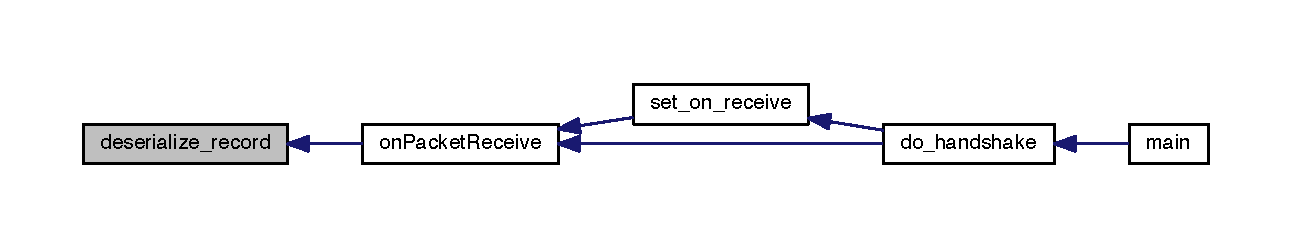
\includegraphics[width=350pt]{_server_client_record_protocol_8h_abb4c45954ce00d016a651588a179ff19_icgraph}
\end{center}
\end{figure}


\index{Server\+Client\+Record\+Protocol.\+h@{Server\+Client\+Record\+Protocol.\+h}!free\+\_\+record@{free\+\_\+record}}
\index{free\+\_\+record@{free\+\_\+record}!Server\+Client\+Record\+Protocol.\+h@{Server\+Client\+Record\+Protocol.\+h}}
\subsubsection[{\texorpdfstring{free\+\_\+record(record\+\_\+t $\ast$r)}{free_record(record_t *r)}}]{\setlength{\rightskip}{0pt plus 5cm}void free\+\_\+record (
\begin{DoxyParamCaption}
\item[{{\bf record\+\_\+t} $\ast$}]{r}
\end{DoxyParamCaption}
)}\hypertarget{_server_client_record_protocol_8h_a9212df7db09a62df2f7d4a913f04defc}{}\label{_server_client_record_protocol_8h_a9212df7db09a62df2f7d4a913f04defc}
Deallocate memory pointed by r 
\begin{DoxyParams}{Parameters}
{\em r} & \+: pointer to record to free \\
\hline
\end{DoxyParams}


Referenced by on\+Packet\+Receive(), and send\+\_\+handshake().



Here is the caller graph for this function\+:\nopagebreak
\begin{figure}[H]
\begin{center}
\leavevmode
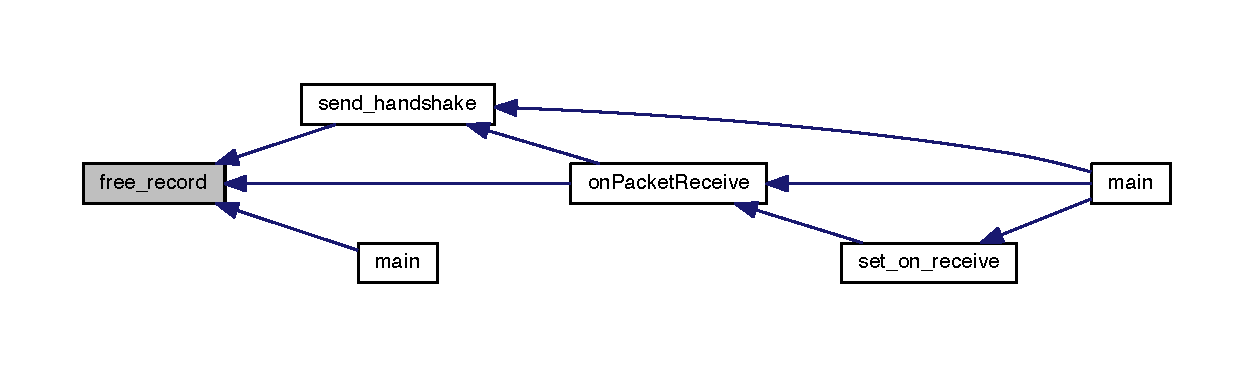
\includegraphics[width=350pt]{_server_client_record_protocol_8h_a9212df7db09a62df2f7d4a913f04defc_icgraph}
\end{center}
\end{figure}


\index{Server\+Client\+Record\+Protocol.\+h@{Server\+Client\+Record\+Protocol.\+h}!print\+\_\+record@{print\+\_\+record}}
\index{print\+\_\+record@{print\+\_\+record}!Server\+Client\+Record\+Protocol.\+h@{Server\+Client\+Record\+Protocol.\+h}}
\subsubsection[{\texorpdfstring{print\+\_\+record(record\+\_\+t $\ast$r)}{print_record(record_t *r)}}]{\setlength{\rightskip}{0pt plus 5cm}void print\+\_\+record (
\begin{DoxyParamCaption}
\item[{{\bf record\+\_\+t} $\ast$}]{r}
\end{DoxyParamCaption}
)}\hypertarget{_server_client_record_protocol_8h_a5029bcdf9f7eb874b25136b76e41963c}{}\label{_server_client_record_protocol_8h_a5029bcdf9f7eb874b25136b76e41963c}
Print a description of the record 
\begin{DoxyParams}{Parameters}
{\em r} & \+: record to print. \\
\hline
\end{DoxyParams}


Referenced by on\+Packet\+Receive(), and print\+\_\+handshake().



Here is the call graph for this function\+:\nopagebreak
\begin{figure}[H]
\begin{center}
\leavevmode
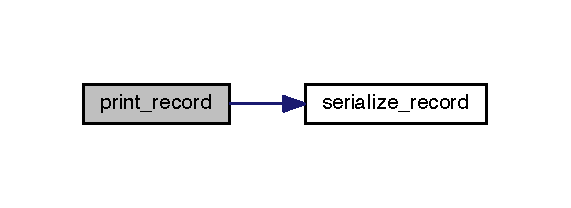
\includegraphics[width=274pt]{_server_client_record_protocol_8h_a5029bcdf9f7eb874b25136b76e41963c_cgraph}
\end{center}
\end{figure}




Here is the caller graph for this function\+:\nopagebreak
\begin{figure}[H]
\begin{center}
\leavevmode
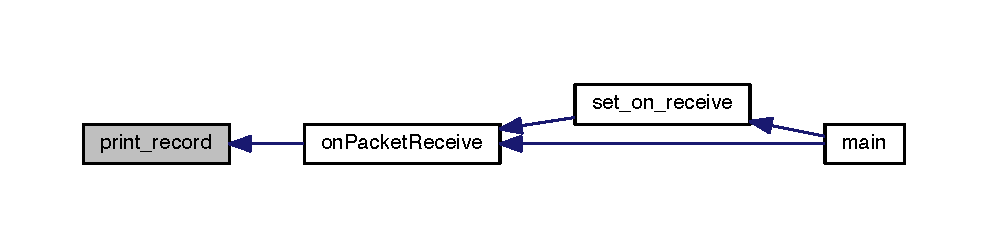
\includegraphics[width=350pt]{_server_client_record_protocol_8h_a5029bcdf9f7eb874b25136b76e41963c_icgraph}
\end{center}
\end{figure}


\index{Server\+Client\+Record\+Protocol.\+h@{Server\+Client\+Record\+Protocol.\+h}!send\+\_\+record@{send\+\_\+record}}
\index{send\+\_\+record@{send\+\_\+record}!Server\+Client\+Record\+Protocol.\+h@{Server\+Client\+Record\+Protocol.\+h}}
\subsubsection[{\texorpdfstring{send\+\_\+record(channel\+\_\+t $\ast$ch, record\+\_\+t $\ast$to\+\_\+send)}{send_record(channel_t *ch, record_t *to_send)}}]{\setlength{\rightskip}{0pt plus 5cm}int send\+\_\+record (
\begin{DoxyParamCaption}
\item[{{\bf channel\+\_\+t} $\ast$}]{ch, }
\item[{{\bf record\+\_\+t} $\ast$}]{r}
\end{DoxyParamCaption}
)}\hypertarget{_server_client_record_protocol_8h_a1ceb817bc488ec68b8abfd289dbbf6c0}{}\label{_server_client_record_protocol_8h_a1ceb817bc488ec68b8abfd289dbbf6c0}
Send record to\+\_\+send over the channel ch. Note \+:for send record is important to set \textquotesingle{}to\textquotesingle{} and \textquotesingle{}from\textquotesingle{} in the channel creation.


\begin{DoxyParams}{Parameters}
{\em ch} & \+: channel to use \\
\hline
{\em to\+\_\+send} & \+: record to send \\
\hline
\end{DoxyParams}
\begin{DoxyReturn}{Returns}
1 if the message was successfully sent, 0 otherwise 
\end{DoxyReturn}


Referenced by on\+Packet\+Receive(), and send\+\_\+handshake().



Here is the call graph for this function\+:\nopagebreak
\begin{figure}[H]
\begin{center}
\leavevmode
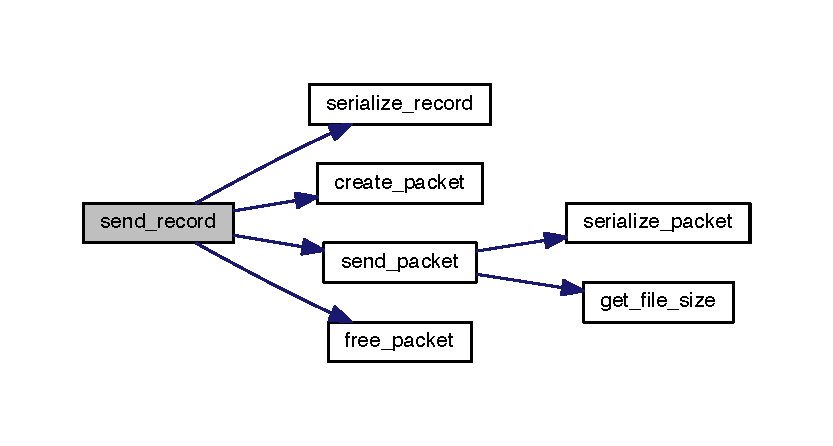
\includegraphics[width=350pt]{_server_client_record_protocol_8h_a1ceb817bc488ec68b8abfd289dbbf6c0_cgraph}
\end{center}
\end{figure}




Here is the caller graph for this function\+:\nopagebreak
\begin{figure}[H]
\begin{center}
\leavevmode
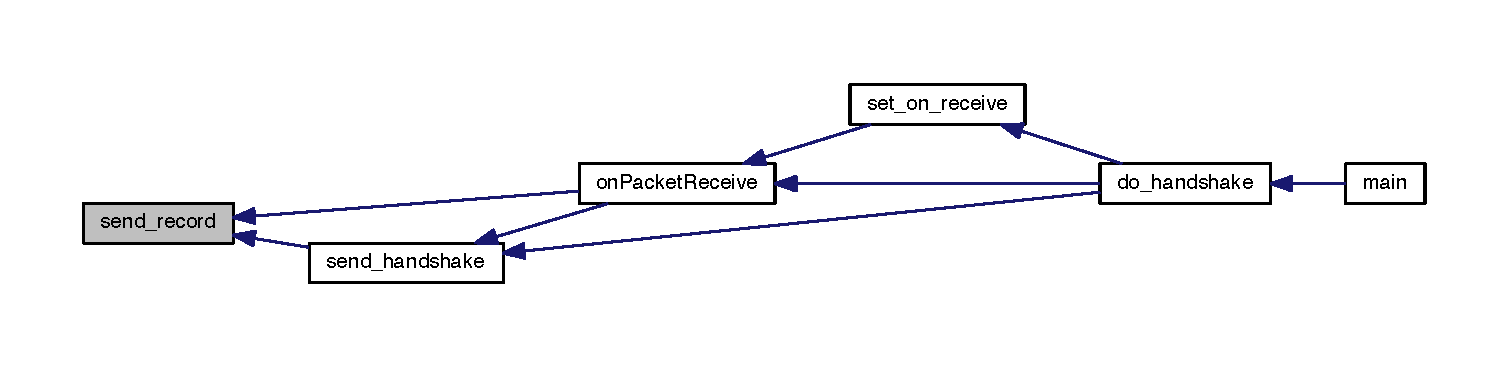
\includegraphics[width=350pt]{_server_client_record_protocol_8h_a1ceb817bc488ec68b8abfd289dbbf6c0_icgraph}
\end{center}
\end{figure}


\index{Server\+Client\+Record\+Protocol.\+h@{Server\+Client\+Record\+Protocol.\+h}!serialize\+\_\+record@{serialize\+\_\+record}}
\index{serialize\+\_\+record@{serialize\+\_\+record}!Server\+Client\+Record\+Protocol.\+h@{Server\+Client\+Record\+Protocol.\+h}}
\subsubsection[{\texorpdfstring{serialize\+\_\+record(record\+\_\+t $\ast$r, unsigned char $\ast$$\ast$message, uint16\+\_\+t $\ast$message\+\_\+len)}{serialize_record(record_t *r, unsigned char **message, uint16_t *message_len)}}]{\setlength{\rightskip}{0pt plus 5cm}void serialize\+\_\+record (
\begin{DoxyParamCaption}
\item[{{\bf record\+\_\+t} $\ast$}]{r, }
\item[{unsigned char $\ast$$\ast$}]{message, }
\item[{uint16\+\_\+t $\ast$}]{message\+Len}
\end{DoxyParamCaption}
)}\hypertarget{_server_client_record_protocol_8h_af6de1ff6a0b52cc2ad9224dbc4e9a14c}{}\label{_server_client_record_protocol_8h_af6de1ff6a0b52cc2ad9224dbc4e9a14c}
Serialize record in a byte stream of length message\+\_\+len stored in message.


\begin{DoxyParams}{Parameters}
{\em message} & \+: pointer to null (the function allocate space for you) \\
\hline
{\em message\+Len} & \+: pointer to integer (will contains the message length) \\
\hline
\end{DoxyParams}


Referenced by print\+\_\+record(), and send\+\_\+record().



Here is the caller graph for this function\+:\nopagebreak
\begin{figure}[H]
\begin{center}
\leavevmode
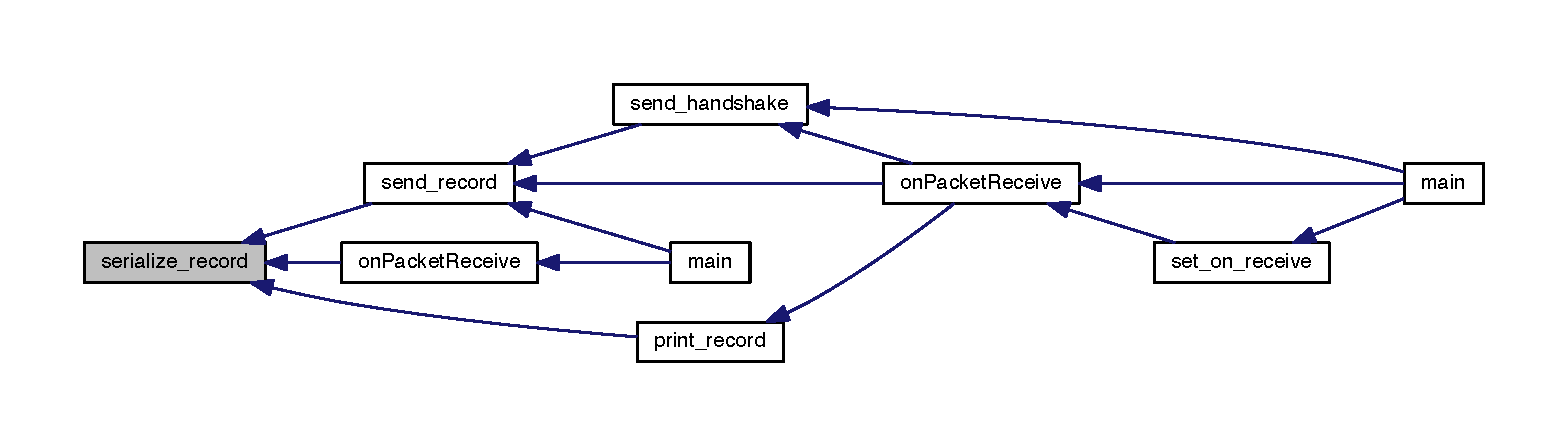
\includegraphics[width=350pt]{_server_client_record_protocol_8h_af6de1ff6a0b52cc2ad9224dbc4e9a14c_icgraph}
\end{center}
\end{figure}



\hypertarget{_server_client_transport_protocol_8h}{}\section{include/\+Server\+Client\+Transport\+Protocol.h File Reference}
\label{_server_client_transport_protocol_8h}\index{include/\+Server\+Client\+Transport\+Protocol.\+h@{include/\+Server\+Client\+Transport\+Protocol.\+h}}
{\ttfamily \#include $<$stdio.\+h$>$}\\*
{\ttfamily \#include $<$stdlib.\+h$>$}\\*
{\ttfamily \#include $<$stdint.\+h$>$}\\*
{\ttfamily \#include $<$string.\+h$>$}\\*
{\ttfamily \#include $<$unistd.\+h$>$}\\*
{\ttfamily \#include $<$sys/wait.\+h$>$}\\*
{\ttfamily \#include $<$sys/file.\+h$>$}\\*
{\ttfamily \#include $<$sys/stat.\+h$>$}\\*
{\ttfamily \#include $<$pthread.\+h$>$}\\*
{\ttfamily \#include $<$time.\+h$>$}\\*
Include dependency graph for Server\+Client\+Transport\+Protocol.\+h\+:
\nopagebreak
\begin{figure}[H]
\begin{center}
\leavevmode
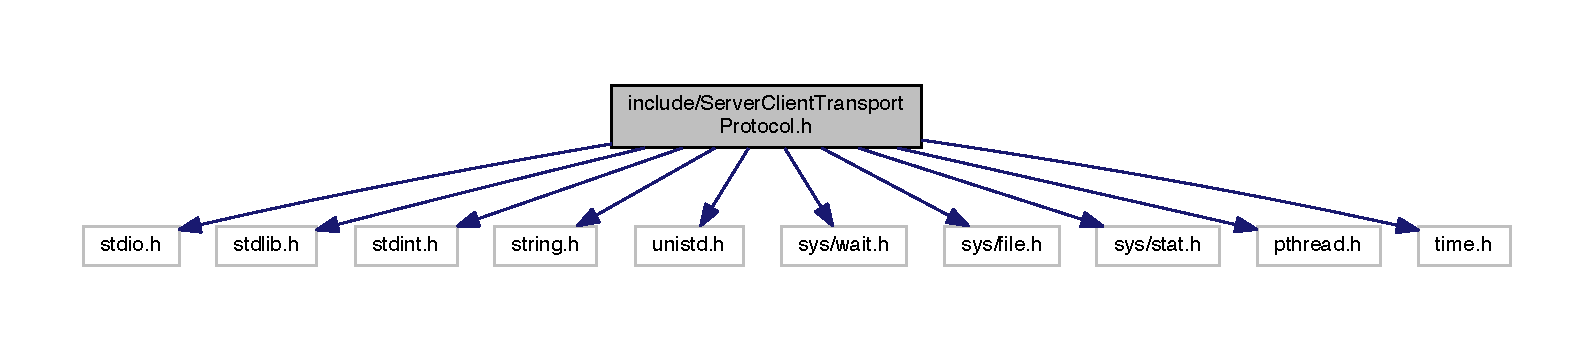
\includegraphics[width=350pt]{_server_client_transport_protocol_8h__incl}
\end{center}
\end{figure}
This graph shows which files directly or indirectly include this file\+:
\nopagebreak
\begin{figure}[H]
\begin{center}
\leavevmode
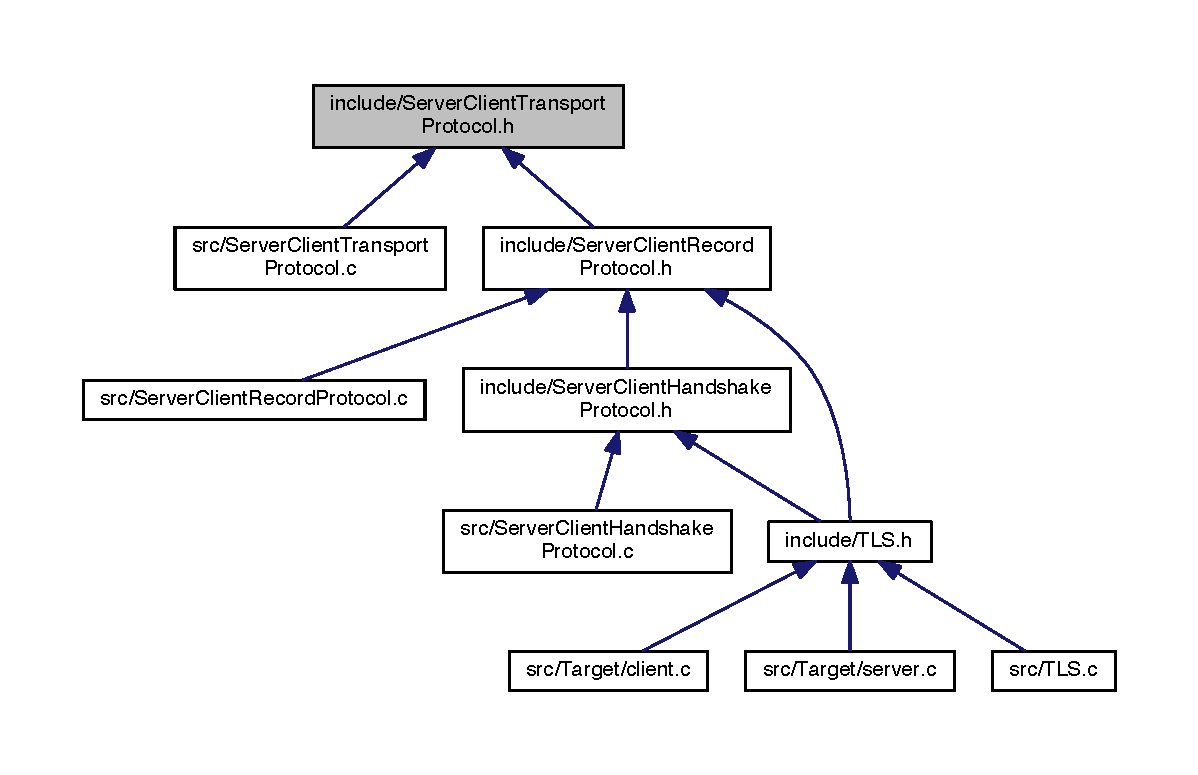
\includegraphics[width=350pt]{_server_client_transport_protocol_8h__dep__incl}
\end{center}
\end{figure}
\subsection*{Data Structures}
\begin{DoxyCompactItemize}
\item 
struct \hyperlink{structpacket__transport__t}{packet\+\_\+transport\+\_\+t}
\item 
struct \hyperlink{structchannel__t}{channel\+\_\+t}
\end{DoxyCompactItemize}
\subsection*{Macros}
\begin{DoxyCompactItemize}
\item 
\#define \hyperlink{_server_client_transport_protocol_8h_a898f8c58e7f9295dcd48d081926f82ca}{D\+E\+L\+A\+Y\+\_\+\+T\+I\+ME}~50
\end{DoxyCompactItemize}
\subsection*{Typedefs}
\begin{DoxyCompactItemize}
\item 
typedef struct \hyperlink{structchannel__t}{channel\+\_\+t} \hyperlink{_server_client_transport_protocol_8h_a23109d98b407095c0ef9fd921ac30b81}{channel\+\_\+t}
\end{DoxyCompactItemize}
\subsection*{Functions}
\begin{DoxyCompactItemize}
\item 
\hyperlink{structchannel__t}{channel\+\_\+t} $\ast$ \hyperlink{_server_client_transport_protocol_8h_aaa07b9b9152780bcb7fbacf14efa7eda}{create\+\_\+channel} (char $\ast$file\+Name, char $\ast$channel\+From, char $\ast$channel\+To)
\item 
int \hyperlink{_server_client_transport_protocol_8h_a018090dd0ba292fbef485142a080fa59}{set\+\_\+on\+\_\+receive} (\hyperlink{structchannel__t}{channel\+\_\+t} $\ast$ch, void($\ast$\hyperlink{server_8c_a98d326f448510d53d67b27e5cbbad82d}{on\+Packet\+Receive})(\hyperlink{structchannel__t}{channel\+\_\+t} $\ast$ch, \hyperlink{structpacket__transport__t}{packet\+\_\+transport\+\_\+t} $\ast$p))
\item 
int \hyperlink{_server_client_transport_protocol_8h_aaf312ea4a4b413a2bbad6f1cd180f4ac}{send\+\_\+packet} (\hyperlink{structchannel__t}{channel\+\_\+t} $\ast$ch, \hyperlink{structpacket__transport__t}{packet\+\_\+transport\+\_\+t} $\ast$p)
\item 
int \hyperlink{_server_client_transport_protocol_8h_ac13189fb7b788d6f0360927759b95a8b}{start\+\_\+listener} (\hyperlink{structchannel__t}{channel\+\_\+t} $\ast$ch)
\item 
void \hyperlink{_server_client_transport_protocol_8h_a771a2acdb87f3679abacac37706d65d7}{wait\+\_\+channel} (\hyperlink{structchannel__t}{channel\+\_\+t} $\ast$ch)
\item 
void \hyperlink{_server_client_transport_protocol_8h_aa8b8d9b75a74ccb0f6a701e16ae8999d}{stop\+\_\+channel} (\hyperlink{structchannel__t}{channel\+\_\+t} $\ast$ch)
\item 
\hyperlink{structpacket__transport__t}{packet\+\_\+transport\+\_\+t} $\ast$ \hyperlink{_server_client_transport_protocol_8h_ab900c15a013c9cb71d24f3e7f5479822}{create\+\_\+packet} (char $\ast$source, char $\ast$destination, unsigned char $\ast$message, uint32\+\_\+t message\+\_\+length)
\item 
void \hyperlink{_server_client_transport_protocol_8h_a52cb1d528c2a550d4d440abeb90e1ea7}{free\+\_\+packet} (\hyperlink{structpacket__transport__t}{packet\+\_\+transport\+\_\+t} $\ast$p)
\end{DoxyCompactItemize}


\subsection{Detailed Description}
S\+S\+L/\+T\+LS Project

Basic client/server communication through file. It substitutes the transport layer in O\+SI stack.

P\+R\+O\+T\+O\+C\+OL\+: The protocol is very simple 8 byte for source 8 byte for receiver 4 byte for packet length message

both server and client after read a message they blank the file both server and client cannot write if the file is not blank, they wait

\begin{DoxyDate}{Date}
Created on 22/12/15. 
\end{DoxyDate}
\begin{DoxyCopyright}{Copyright}
Copyright © 2015 Alessandro Melloni, Andrea Francesco Vinci. All rights reserved. 
\end{DoxyCopyright}


\subsection{Macro Definition Documentation}
\index{Server\+Client\+Transport\+Protocol.\+h@{Server\+Client\+Transport\+Protocol.\+h}!D\+E\+L\+A\+Y\+\_\+\+T\+I\+ME@{D\+E\+L\+A\+Y\+\_\+\+T\+I\+ME}}
\index{D\+E\+L\+A\+Y\+\_\+\+T\+I\+ME@{D\+E\+L\+A\+Y\+\_\+\+T\+I\+ME}!Server\+Client\+Transport\+Protocol.\+h@{Server\+Client\+Transport\+Protocol.\+h}}
\subsubsection[{\texorpdfstring{D\+E\+L\+A\+Y\+\_\+\+T\+I\+ME}{DELAY_TIME}}]{\setlength{\rightskip}{0pt plus 5cm}\#define D\+E\+L\+A\+Y\+\_\+\+T\+I\+ME~50}\hypertarget{_server_client_transport_protocol_8h_a898f8c58e7f9295dcd48d081926f82ca}{}\label{_server_client_transport_protocol_8h_a898f8c58e7f9295dcd48d081926f82ca}


Referenced by reader().



\subsection{Typedef Documentation}
\index{Server\+Client\+Transport\+Protocol.\+h@{Server\+Client\+Transport\+Protocol.\+h}!channel\+\_\+t@{channel\+\_\+t}}
\index{channel\+\_\+t@{channel\+\_\+t}!Server\+Client\+Transport\+Protocol.\+h@{Server\+Client\+Transport\+Protocol.\+h}}
\subsubsection[{\texorpdfstring{channel\+\_\+t}{channel_t}}]{\setlength{\rightskip}{0pt plus 5cm}typedef struct {\bf channel\+\_\+t} {\bf channel\+\_\+t}}\hypertarget{_server_client_transport_protocol_8h_a23109d98b407095c0ef9fd921ac30b81}{}\label{_server_client_transport_protocol_8h_a23109d98b407095c0ef9fd921ac30b81}


\subsection{Function Documentation}
\index{Server\+Client\+Transport\+Protocol.\+h@{Server\+Client\+Transport\+Protocol.\+h}!create\+\_\+channel@{create\+\_\+channel}}
\index{create\+\_\+channel@{create\+\_\+channel}!Server\+Client\+Transport\+Protocol.\+h@{Server\+Client\+Transport\+Protocol.\+h}}
\subsubsection[{\texorpdfstring{create\+\_\+channel(char $\ast$file\+Name, char $\ast$channel\+From, char $\ast$channel\+To)}{create_channel(char *fileName, char *channelFrom, char *channelTo)}}]{\setlength{\rightskip}{0pt plus 5cm}{\bf channel\+\_\+t}$\ast$ create\+\_\+channel (
\begin{DoxyParamCaption}
\item[{char $\ast$}]{file\+Name, }
\item[{char $\ast$}]{channel\+From, }
\item[{char $\ast$}]{channel\+To}
\end{DoxyParamCaption}
)}\hypertarget{_server_client_transport_protocol_8h_aaa07b9b9152780bcb7fbacf14efa7eda}{}\label{_server_client_transport_protocol_8h_aaa07b9b9152780bcb7fbacf14efa7eda}
Create a server/client channel using the file\+Name as comunication channel


\begin{DoxyParams}{Parameters}
{\em file\+Name} & \+: file name of the channel \\
\hline
{\em server\+Name} & \+: name of the server/client \\
\hline
\end{DoxyParams}
\begin{DoxyReturn}{Returns}
the created channel 
\end{DoxyReturn}


Referenced by do\+\_\+handshake().



Here is the caller graph for this function\+:\nopagebreak
\begin{figure}[H]
\begin{center}
\leavevmode
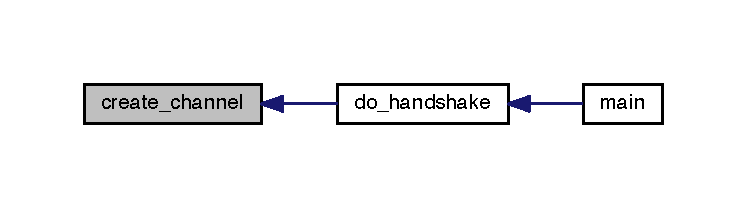
\includegraphics[width=350pt]{_server_client_transport_protocol_8h_aaa07b9b9152780bcb7fbacf14efa7eda_icgraph}
\end{center}
\end{figure}


\index{Server\+Client\+Transport\+Protocol.\+h@{Server\+Client\+Transport\+Protocol.\+h}!create\+\_\+packet@{create\+\_\+packet}}
\index{create\+\_\+packet@{create\+\_\+packet}!Server\+Client\+Transport\+Protocol.\+h@{Server\+Client\+Transport\+Protocol.\+h}}
\subsubsection[{\texorpdfstring{create\+\_\+packet(char $\ast$source, char $\ast$destination, unsigned char $\ast$message, uint32\+\_\+t message\+\_\+length)}{create_packet(char *source, char *destination, unsigned char *message, uint32_t message_length)}}]{\setlength{\rightskip}{0pt plus 5cm}{\bf packet\+\_\+transport\+\_\+t}$\ast$ create\+\_\+packet (
\begin{DoxyParamCaption}
\item[{char $\ast$}]{source, }
\item[{char $\ast$}]{destination, }
\item[{unsigned char $\ast$}]{message, }
\item[{uint32\+\_\+t}]{message\+\_\+length}
\end{DoxyParamCaption}
)}\hypertarget{_server_client_transport_protocol_8h_ab900c15a013c9cb71d24f3e7f5479822}{}\label{_server_client_transport_protocol_8h_ab900c15a013c9cb71d24f3e7f5479822}
Create a packet starting from a byte stream source and destination


\begin{DoxyParams}{Parameters}
{\em source} & \+: packet source \\
\hline
{\em destination} & \+: packet receiver \\
\hline
{\em message} & \+: message stream to be encapsulate into packet \\
\hline
{\em message\+\_\+length} & message lenght \\
\hline
\end{DoxyParams}
\begin{DoxyReturn}{Returns}
a pointer to a builded packet 
\end{DoxyReturn}


Referenced by deserialize\+\_\+packet(), and send\+\_\+record().



Here is the caller graph for this function\+:\nopagebreak
\begin{figure}[H]
\begin{center}
\leavevmode
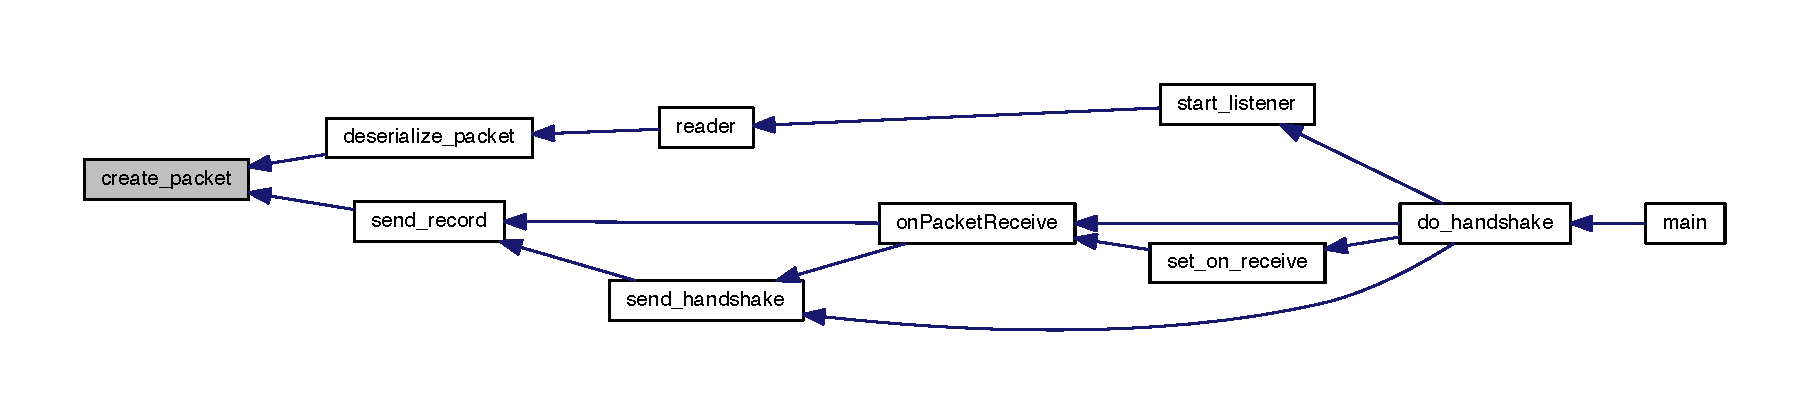
\includegraphics[width=350pt]{_server_client_transport_protocol_8h_ab900c15a013c9cb71d24f3e7f5479822_icgraph}
\end{center}
\end{figure}


\index{Server\+Client\+Transport\+Protocol.\+h@{Server\+Client\+Transport\+Protocol.\+h}!free\+\_\+packet@{free\+\_\+packet}}
\index{free\+\_\+packet@{free\+\_\+packet}!Server\+Client\+Transport\+Protocol.\+h@{Server\+Client\+Transport\+Protocol.\+h}}
\subsubsection[{\texorpdfstring{free\+\_\+packet(packet\+\_\+transport\+\_\+t $\ast$p)}{free_packet(packet_transport_t *p)}}]{\setlength{\rightskip}{0pt plus 5cm}void free\+\_\+packet (
\begin{DoxyParamCaption}
\item[{{\bf packet\+\_\+transport\+\_\+t} $\ast$}]{p}
\end{DoxyParamCaption}
)}\hypertarget{_server_client_transport_protocol_8h_a52cb1d528c2a550d4d440abeb90e1ea7}{}\label{_server_client_transport_protocol_8h_a52cb1d528c2a550d4d440abeb90e1ea7}
Deallocate memory allocated by packet 
\begin{DoxyParams}{Parameters}
{\em p} & \+: pointer to packet to free \\
\hline
\end{DoxyParams}


Referenced by on\+Packet\+Receive(), reader(), and send\+\_\+record().



Here is the caller graph for this function\+:\nopagebreak
\begin{figure}[H]
\begin{center}
\leavevmode
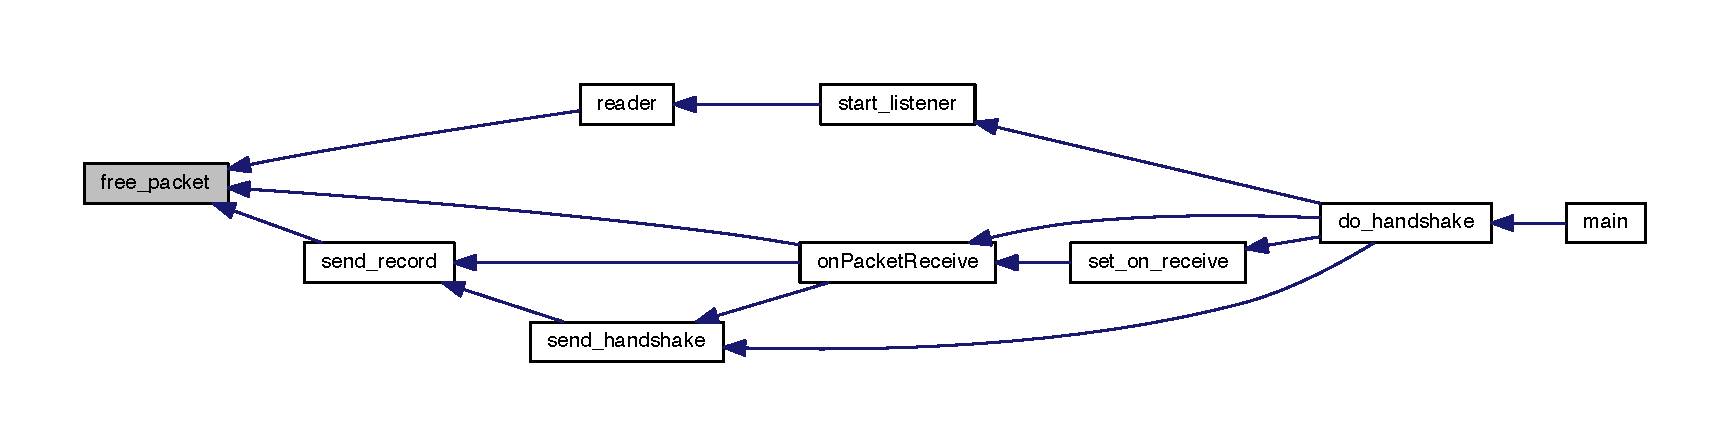
\includegraphics[width=350pt]{_server_client_transport_protocol_8h_a52cb1d528c2a550d4d440abeb90e1ea7_icgraph}
\end{center}
\end{figure}


\index{Server\+Client\+Transport\+Protocol.\+h@{Server\+Client\+Transport\+Protocol.\+h}!send\+\_\+packet@{send\+\_\+packet}}
\index{send\+\_\+packet@{send\+\_\+packet}!Server\+Client\+Transport\+Protocol.\+h@{Server\+Client\+Transport\+Protocol.\+h}}
\subsubsection[{\texorpdfstring{send\+\_\+packet(channel\+\_\+t $\ast$ch, packet\+\_\+transport\+\_\+t $\ast$p)}{send_packet(channel_t *ch, packet_transport_t *p)}}]{\setlength{\rightskip}{0pt plus 5cm}int send\+\_\+packet (
\begin{DoxyParamCaption}
\item[{{\bf channel\+\_\+t} $\ast$}]{ch, }
\item[{{\bf packet\+\_\+transport\+\_\+t} $\ast$}]{p}
\end{DoxyParamCaption}
)}\hypertarget{_server_client_transport_protocol_8h_aaf312ea4a4b413a2bbad6f1cd180f4ac}{}\label{_server_client_transport_protocol_8h_aaf312ea4a4b413a2bbad6f1cd180f4ac}
Send a message trough the channel ch


\begin{DoxyParams}{Parameters}
{\em ch} & \+: channel to be used \\
\hline
{\em p} & \+: pointer to packet to be sent \\
\hline
\end{DoxyParams}
\begin{DoxyReturn}{Returns}
\+: 1 if the message was sent, 0 otherwise 
\end{DoxyReturn}


Referenced by send\+\_\+record().



Here is the call graph for this function\+:\nopagebreak
\begin{figure}[H]
\begin{center}
\leavevmode
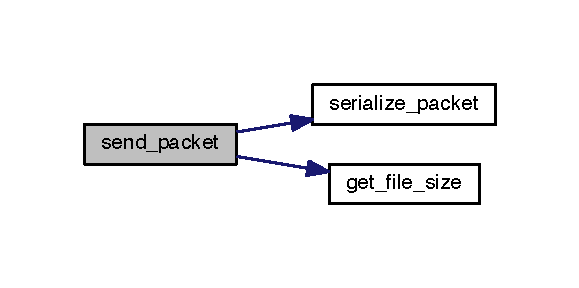
\includegraphics[width=278pt]{_server_client_transport_protocol_8h_aaf312ea4a4b413a2bbad6f1cd180f4ac_cgraph}
\end{center}
\end{figure}




Here is the caller graph for this function\+:\nopagebreak
\begin{figure}[H]
\begin{center}
\leavevmode
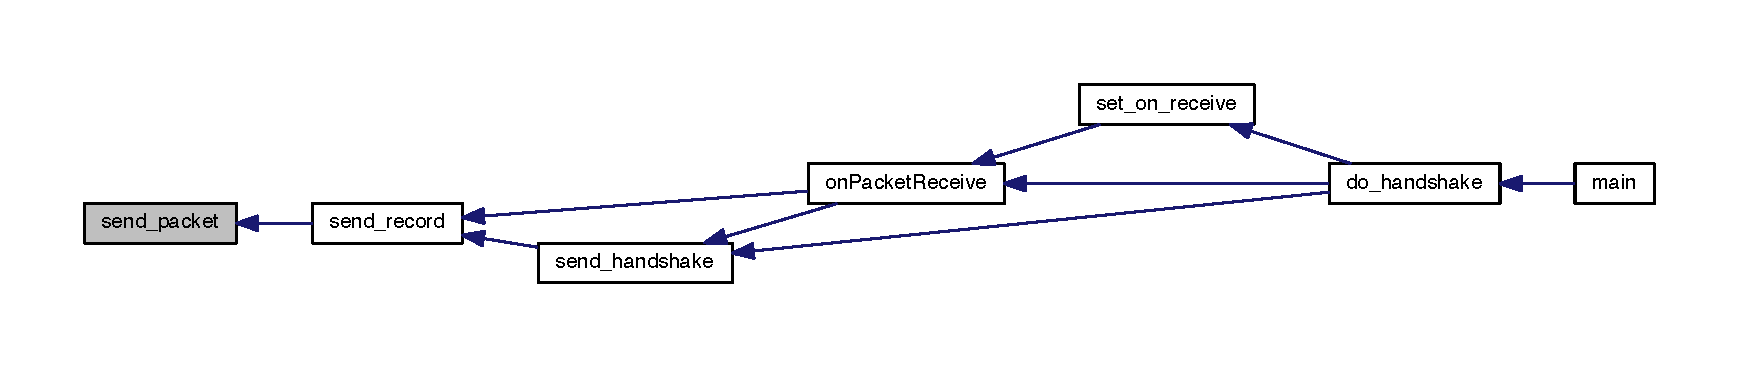
\includegraphics[width=350pt]{_server_client_transport_protocol_8h_aaf312ea4a4b413a2bbad6f1cd180f4ac_icgraph}
\end{center}
\end{figure}


\index{Server\+Client\+Transport\+Protocol.\+h@{Server\+Client\+Transport\+Protocol.\+h}!set\+\_\+on\+\_\+receive@{set\+\_\+on\+\_\+receive}}
\index{set\+\_\+on\+\_\+receive@{set\+\_\+on\+\_\+receive}!Server\+Client\+Transport\+Protocol.\+h@{Server\+Client\+Transport\+Protocol.\+h}}
\subsubsection[{\texorpdfstring{set\+\_\+on\+\_\+receive(channel\+\_\+t $\ast$ch, void($\ast$on\+Packet\+Receive)(channel\+\_\+t $\ast$ch, packet\+\_\+transport\+\_\+t $\ast$p))}{set_on_receive(channel_t *ch, void(*onPacketReceive)(channel_t *ch, packet_transport_t *p))}}]{\setlength{\rightskip}{0pt plus 5cm}int set\+\_\+on\+\_\+receive (
\begin{DoxyParamCaption}
\item[{{\bf channel\+\_\+t} $\ast$}]{ch, }
\item[{void($\ast$)({\bf channel\+\_\+t} $\ast$ch, {\bf packet\+\_\+transport\+\_\+t} $\ast$p)}]{on\+Packet\+Receive}
\end{DoxyParamCaption}
)}\hypertarget{_server_client_transport_protocol_8h_a018090dd0ba292fbef485142a080fa59}{}\label{_server_client_transport_protocol_8h_a018090dd0ba292fbef485142a080fa59}
Set the function to be called when a message is received


\begin{DoxyParams}{Parameters}
{\em ch} & \+: channel interested \\
\hline
{\em on\+Packet\+Receive} & \+: pointer to the function to be called \\
\hline
\end{DoxyParams}
\begin{DoxyReturn}{Returns}
\+: 1 if the function was setted, 0 otherwise 
\end{DoxyReturn}


Referenced by do\+\_\+handshake().



Here is the call graph for this function\+:\nopagebreak
\begin{figure}[H]
\begin{center}
\leavevmode
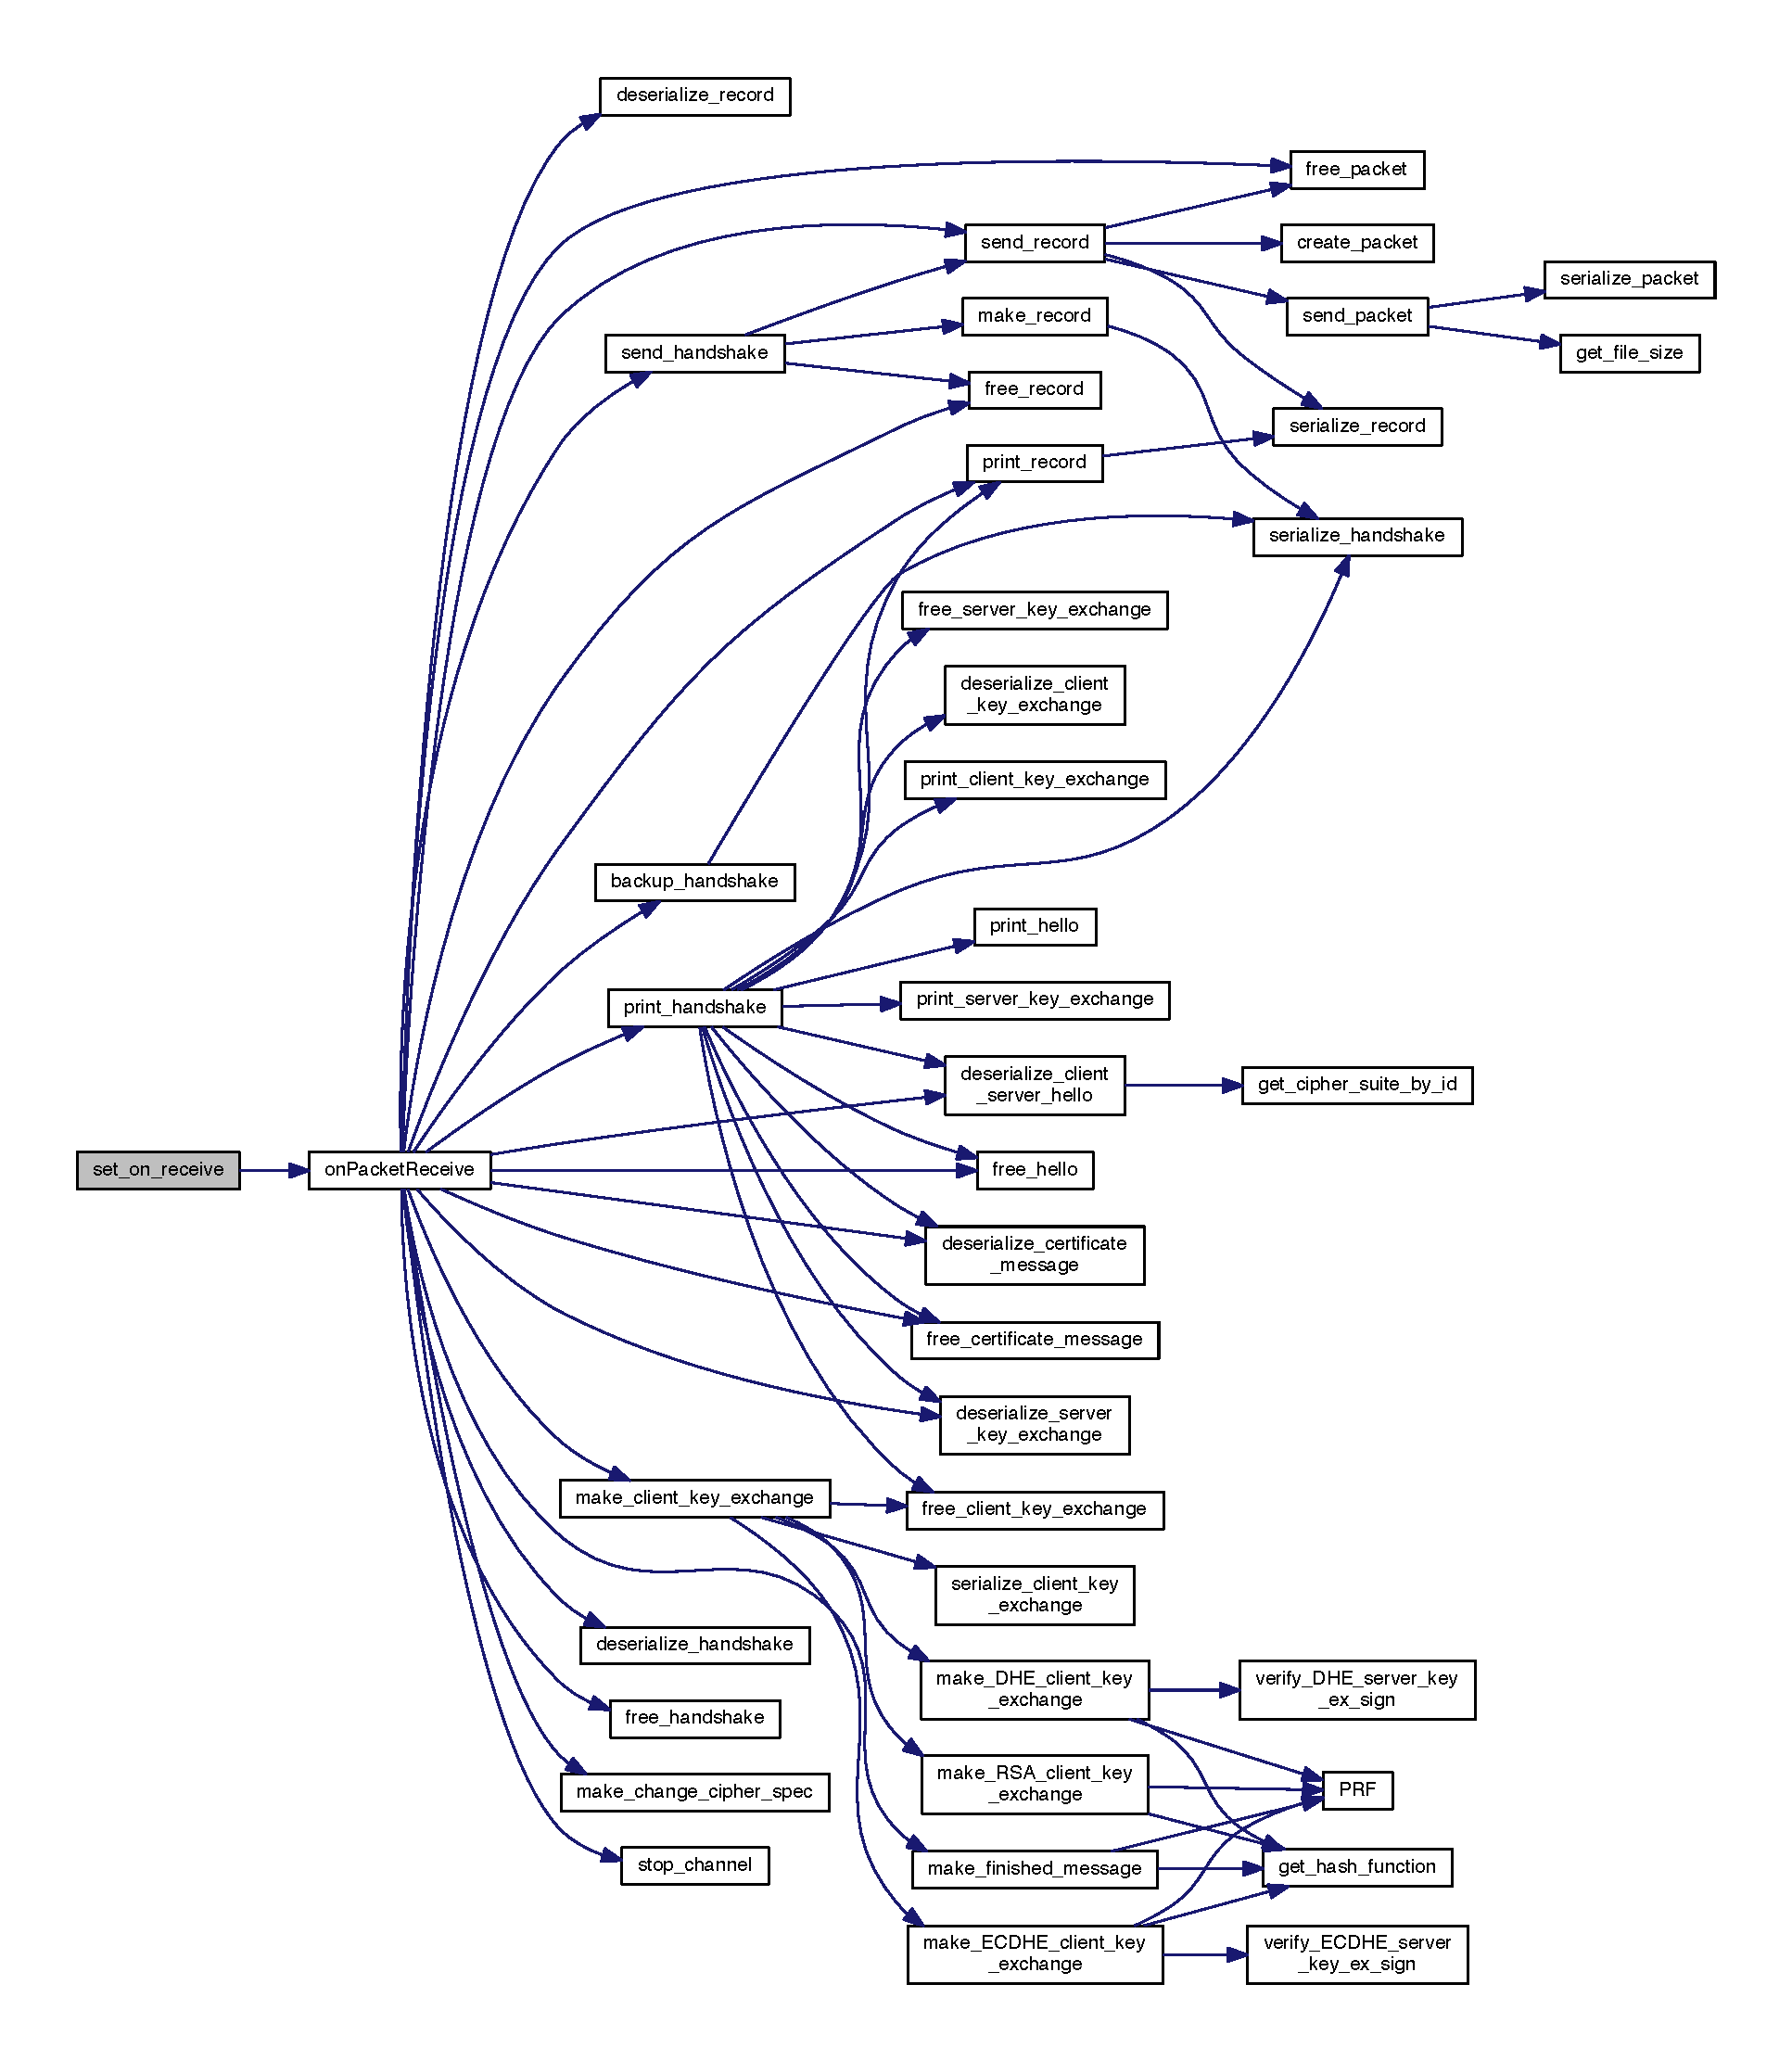
\includegraphics[width=350pt]{_server_client_transport_protocol_8h_a018090dd0ba292fbef485142a080fa59_cgraph}
\end{center}
\end{figure}




Here is the caller graph for this function\+:\nopagebreak
\begin{figure}[H]
\begin{center}
\leavevmode
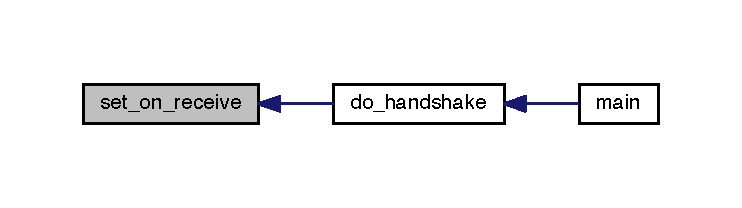
\includegraphics[width=350pt]{_server_client_transport_protocol_8h_a018090dd0ba292fbef485142a080fa59_icgraph}
\end{center}
\end{figure}


\index{Server\+Client\+Transport\+Protocol.\+h@{Server\+Client\+Transport\+Protocol.\+h}!start\+\_\+listener@{start\+\_\+listener}}
\index{start\+\_\+listener@{start\+\_\+listener}!Server\+Client\+Transport\+Protocol.\+h@{Server\+Client\+Transport\+Protocol.\+h}}
\subsubsection[{\texorpdfstring{start\+\_\+listener(channel\+\_\+t $\ast$ch)}{start_listener(channel_t *ch)}}]{\setlength{\rightskip}{0pt plus 5cm}int start\+\_\+listener (
\begin{DoxyParamCaption}
\item[{{\bf channel\+\_\+t} $\ast$}]{ch}
\end{DoxyParamCaption}
)}\hypertarget{_server_client_transport_protocol_8h_ac13189fb7b788d6f0360927759b95a8b}{}\label{_server_client_transport_protocol_8h_ac13189fb7b788d6f0360927759b95a8b}
Start the channel. We open another thread for the reading and the current thread for writing. From now on (if the operation is succesfull) the client/server read continously from channel. (for S\+T\+OP use stop())


\begin{DoxyParams}{Parameters}
{\em ch} & \+: channel to start \\
\hline
\end{DoxyParams}
\begin{DoxyReturn}{Returns}
\+: 1 if the thread was started, 0 otherwise 
\end{DoxyReturn}


Referenced by do\+\_\+handshake().



Here is the call graph for this function\+:\nopagebreak
\begin{figure}[H]
\begin{center}
\leavevmode
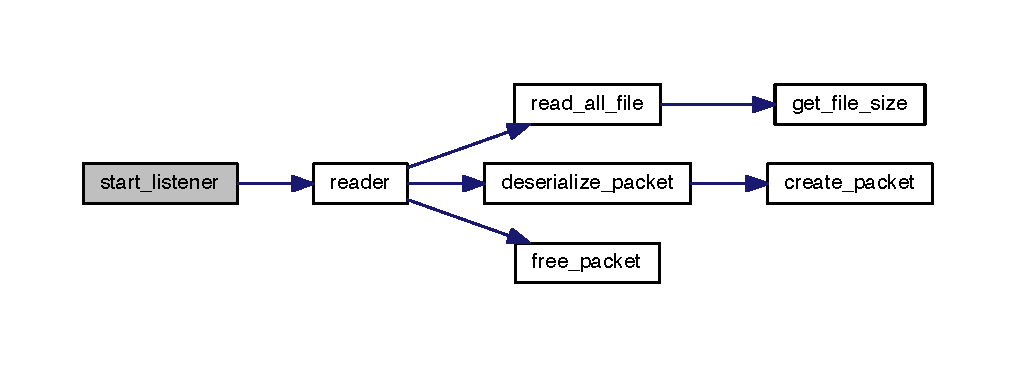
\includegraphics[width=350pt]{_server_client_transport_protocol_8h_ac13189fb7b788d6f0360927759b95a8b_cgraph}
\end{center}
\end{figure}




Here is the caller graph for this function\+:\nopagebreak
\begin{figure}[H]
\begin{center}
\leavevmode
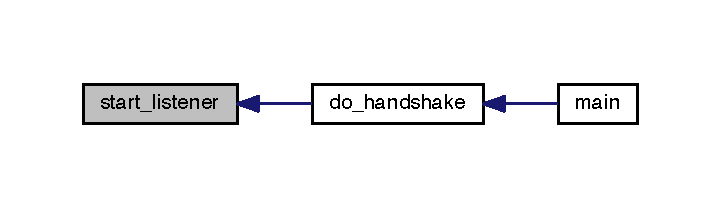
\includegraphics[width=346pt]{_server_client_transport_protocol_8h_ac13189fb7b788d6f0360927759b95a8b_icgraph}
\end{center}
\end{figure}


\index{Server\+Client\+Transport\+Protocol.\+h@{Server\+Client\+Transport\+Protocol.\+h}!stop\+\_\+channel@{stop\+\_\+channel}}
\index{stop\+\_\+channel@{stop\+\_\+channel}!Server\+Client\+Transport\+Protocol.\+h@{Server\+Client\+Transport\+Protocol.\+h}}
\subsubsection[{\texorpdfstring{stop\+\_\+channel(channel\+\_\+t $\ast$ch)}{stop_channel(channel_t *ch)}}]{\setlength{\rightskip}{0pt plus 5cm}void stop\+\_\+channel (
\begin{DoxyParamCaption}
\item[{{\bf channel\+\_\+t} $\ast$}]{ch}
\end{DoxyParamCaption}
)}\hypertarget{_server_client_transport_protocol_8h_aa8b8d9b75a74ccb0f6a701e16ae8999d}{}\label{_server_client_transport_protocol_8h_aa8b8d9b75a74ccb0f6a701e16ae8999d}
Stop the reading/write thread and the channel. Note\+: the function doesn\textquotesingle{}t free the channel. 
\begin{DoxyParams}{Parameters}
{\em ch} & \+: channel to stop \\
\hline
\end{DoxyParams}


Referenced by on\+Packet\+Receive().



Here is the caller graph for this function\+:\nopagebreak
\begin{figure}[H]
\begin{center}
\leavevmode
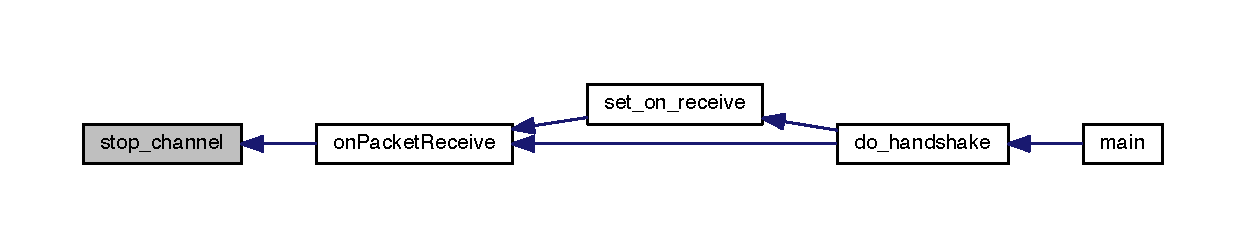
\includegraphics[width=350pt]{_server_client_transport_protocol_8h_aa8b8d9b75a74ccb0f6a701e16ae8999d_icgraph}
\end{center}
\end{figure}


\index{Server\+Client\+Transport\+Protocol.\+h@{Server\+Client\+Transport\+Protocol.\+h}!wait\+\_\+channel@{wait\+\_\+channel}}
\index{wait\+\_\+channel@{wait\+\_\+channel}!Server\+Client\+Transport\+Protocol.\+h@{Server\+Client\+Transport\+Protocol.\+h}}
\subsubsection[{\texorpdfstring{wait\+\_\+channel(channel\+\_\+t $\ast$ch)}{wait_channel(channel_t *ch)}}]{\setlength{\rightskip}{0pt plus 5cm}void wait\+\_\+channel (
\begin{DoxyParamCaption}
\item[{{\bf channel\+\_\+t} $\ast$}]{ch}
\end{DoxyParamCaption}
)}\hypertarget{_server_client_transport_protocol_8h_a771a2acdb87f3679abacac37706d65d7}{}\label{_server_client_transport_protocol_8h_a771a2acdb87f3679abacac37706d65d7}
Stop the callee and wait untill stop is called 
\begin{DoxyParams}{Parameters}
{\em ch} & \+: the chanal to wait \\
\hline
\end{DoxyParams}


Referenced by do\+\_\+handshake().



Here is the caller graph for this function\+:\nopagebreak
\begin{figure}[H]
\begin{center}
\leavevmode
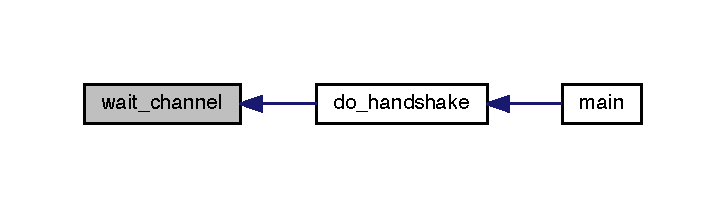
\includegraphics[width=348pt]{_server_client_transport_protocol_8h_a771a2acdb87f3679abacac37706d65d7_icgraph}
\end{center}
\end{figure}



\hypertarget{_t_l_s_8h}{}\section{include/\+T\+LS.h File Reference}
\label{_t_l_s_8h}\index{include/\+T\+L\+S.\+h@{include/\+T\+L\+S.\+h}}
{\ttfamily \#include $<$stdio.\+h$>$}\\*
{\ttfamily \#include $<$time.\+h$>$}\\*
{\ttfamily \#include \char`\"{}Server\+Client\+Handshake\+Protocol.\+h\char`\"{}}\\*
{\ttfamily \#include \char`\"{}Server\+Client\+Record\+Protocol.\+h\char`\"{}}\\*
{\ttfamily \#include \char`\"{}Crypto.\+h\char`\"{}}\\*
Include dependency graph for T\+L\+S.\+h\+:
\nopagebreak
\begin{figure}[H]
\begin{center}
\leavevmode
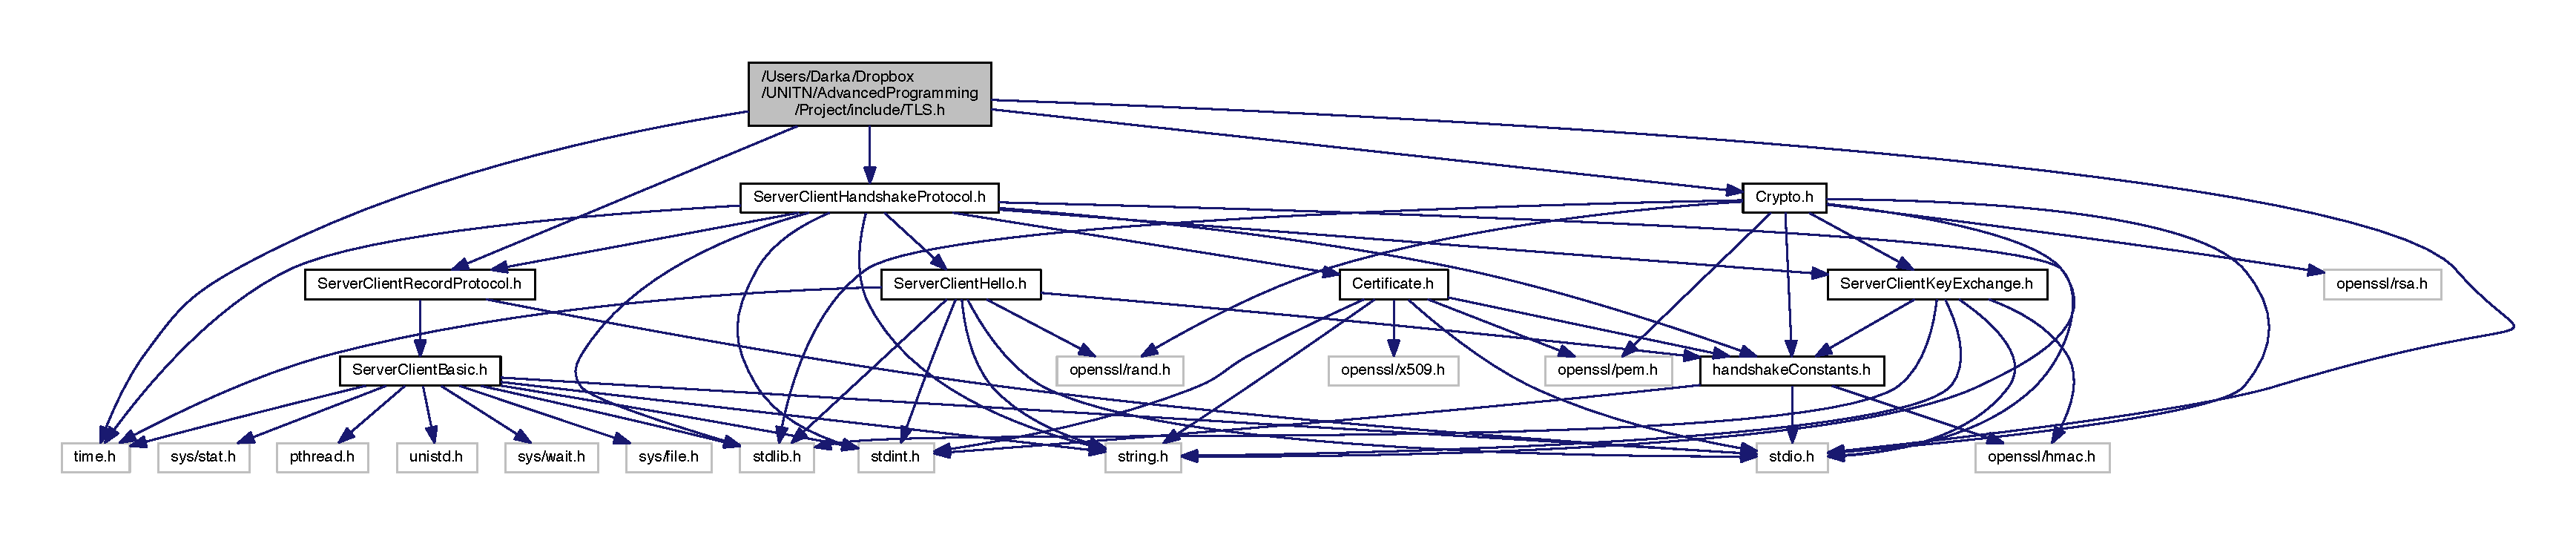
\includegraphics[width=350pt]{_t_l_s_8h__incl}
\end{center}
\end{figure}
This graph shows which files directly or indirectly include this file\+:
\nopagebreak
\begin{figure}[H]
\begin{center}
\leavevmode
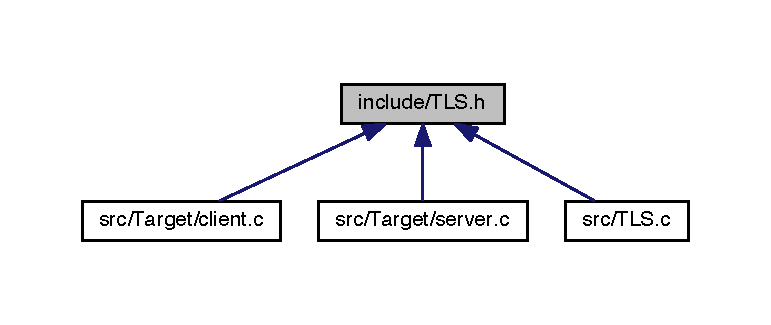
\includegraphics[width=350pt]{_t_l_s_8h__dep__incl}
\end{center}
\end{figure}
\subsection*{Data Structures}
\begin{DoxyCompactItemize}
\item 
struct \hyperlink{struct_t_l_s__parameters__t}{T\+L\+S\+\_\+parameters\+\_\+t}
\end{DoxyCompactItemize}
\subsection*{Functions}
\begin{DoxyCompactItemize}
\item 
\hyperlink{structhandshake__t}{handshake\+\_\+t} $\ast$ \hyperlink{_t_l_s_8h_a7c6bc0a015a0a78cb508614995b9172e}{make\+\_\+client\+\_\+hello} (unsigned char $\ast$client\+\_\+random, \hyperlink{structcipher__suite__t}{cipher\+\_\+suite\+\_\+t} \hyperlink{_t_l_s_constants_8c_ace4b851fd953c51fe7b0ada522a95ae3}{cipher\+\_\+suite\+\_\+list}\mbox{[}$\,$\mbox{]}, int cipher\+\_\+suite\+\_\+len)
\item 
\hyperlink{structhandshake__t}{handshake\+\_\+t} $\ast$ \hyperlink{_t_l_s_8h_ab3bb4e3f75fb84baa35cd0931381dfe0}{make\+\_\+client\+\_\+key\+\_\+exchange} (\hyperlink{struct_t_l_s__parameters__t}{T\+L\+S\+\_\+parameters\+\_\+t} $\ast$\hyperlink{server_8c_aa8eef32066e04e25183a0cc549992c54}{T\+L\+S\+\_\+param}, uint16\+\_\+t key\+\_\+ex\+\_\+alg)
\item 
\hyperlink{structrecord__t}{record\+\_\+t} $\ast$ \hyperlink{_t_l_s_8h_a5bed323f749e27db36fd6ab2a3e64c4a}{make\+\_\+change\+\_\+cipher\+\_\+spec} ()
\item 
\hyperlink{structhandshake__t}{handshake\+\_\+t} $\ast$ \hyperlink{_t_l_s_8h_ae149244e09cbbd2180bc4c5fc6d0a924}{make\+\_\+finished\+\_\+message} (\hyperlink{struct_t_l_s__parameters__t}{T\+L\+S\+\_\+parameters\+\_\+t} $\ast$\hyperlink{server_8c_aa8eef32066e04e25183a0cc549992c54}{T\+L\+S\+\_\+param})
\item 
\hyperlink{structhandshake__t}{handshake\+\_\+t} $\ast$ \hyperlink{_t_l_s_8h_a035a830fd89c6c7af60809197d81ea29}{make\+\_\+server\+\_\+hello} (\hyperlink{struct_t_l_s__parameters__t}{T\+L\+S\+\_\+parameters\+\_\+t} $\ast$\hyperlink{server_8c_aa8eef32066e04e25183a0cc549992c54}{T\+L\+S\+\_\+param}, \hyperlink{structserver__client__hello__t}{server\+\_\+client\+\_\+hello\+\_\+t} $\ast$client\+\_\+hello)
\item 
\hyperlink{structhandshake__t}{handshake\+\_\+t} $\ast$ \hyperlink{_t_l_s_8h_a6fd919275c5d6d3e6578c480cc62a8ce}{make\+\_\+certificate} (\hyperlink{struct_t_l_s__parameters__t}{T\+L\+S\+\_\+parameters\+\_\+t} $\ast$\hyperlink{server_8c_aa8eef32066e04e25183a0cc549992c54}{T\+L\+S\+\_\+param})
\item 
\hyperlink{structhandshake__t}{handshake\+\_\+t} $\ast$ \hyperlink{_t_l_s_8h_a902d940508d7080023ef072b2667a143}{make\+\_\+server\+\_\+key\+\_\+exchange} (\hyperlink{struct_t_l_s__parameters__t}{T\+L\+S\+\_\+parameters\+\_\+t} $\ast$\hyperlink{server_8c_aa8eef32066e04e25183a0cc549992c54}{T\+L\+S\+\_\+param})
\item 
\hyperlink{structhandshake__t}{handshake\+\_\+t} $\ast$ \hyperlink{_t_l_s_8h_af98aa49e2563d588c366ef1712de925a}{make\+\_\+server\+\_\+hello\+\_\+done} ()
\item 
void \hyperlink{_t_l_s_8h_a12a63a5becca8f85a59f6ac0f4d9c553}{backup\+\_\+handshake} (\hyperlink{struct_t_l_s__parameters__t}{T\+L\+S\+\_\+parameters\+\_\+t} $\ast$\hyperlink{server_8c_aa8eef32066e04e25183a0cc549992c54}{T\+L\+S\+\_\+param}, \hyperlink{structhandshake__t}{handshake\+\_\+t} $\ast$h)
\end{DoxyCompactItemize}


\subsection{Detailed Description}
S\+S\+L/\+T\+LS Project

This file provide a set of function for the T\+LS handshake. The function are used for make T\+LS message for both server and client.

\begin{DoxyDate}{Date}
Created on 13/01/16. 
\end{DoxyDate}
\begin{DoxyCopyright}{Copyright}
Copyright © 2016 Alessandro Melloni, Andrea Francesco Vinci. All rights reserved. 
\end{DoxyCopyright}


\subsection{Function Documentation}
\index{T\+L\+S.\+h@{T\+L\+S.\+h}!backup\+\_\+handshake@{backup\+\_\+handshake}}
\index{backup\+\_\+handshake@{backup\+\_\+handshake}!T\+L\+S.\+h@{T\+L\+S.\+h}}
\subsubsection[{\texorpdfstring{backup\+\_\+handshake(\+T\+L\+S\+\_\+parameters\+\_\+t $\ast$\+T\+L\+S\+\_\+param, handshake\+\_\+t $\ast$h)}{backup_handshake(TLS_parameters_t *TLS_param, handshake_t *h)}}]{\setlength{\rightskip}{0pt plus 5cm}void backup\+\_\+handshake (
\begin{DoxyParamCaption}
\item[{{\bf T\+L\+S\+\_\+parameters\+\_\+t} $\ast$}]{T\+L\+S\+\_\+param, }
\item[{{\bf handshake\+\_\+t} $\ast$}]{h}
\end{DoxyParamCaption}
)}\hypertarget{_t_l_s_8h_a12a63a5becca8f85a59f6ac0f4d9c553}{}\label{_t_l_s_8h_a12a63a5becca8f85a59f6ac0f4d9c553}
Append the handshake h to the handshake\+\_\+messages field of T\+L\+S\+\_\+param


\begin{DoxyParams}{Parameters}
{\em T\+L\+S\+\_\+param} & \+: connection parameters \\
\hline
{\em h} & \+: the handshake to append \\
\hline
\end{DoxyParams}


Referenced by do\+\_\+handshake(), and on\+Packet\+Receive().



Here is the call graph for this function\+:\nopagebreak
\begin{figure}[H]
\begin{center}
\leavevmode
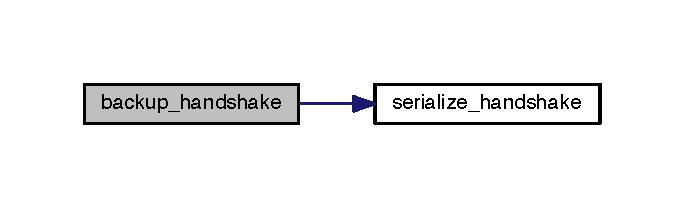
\includegraphics[width=328pt]{_t_l_s_8h_a12a63a5becca8f85a59f6ac0f4d9c553_cgraph}
\end{center}
\end{figure}




Here is the caller graph for this function\+:\nopagebreak
\begin{figure}[H]
\begin{center}
\leavevmode
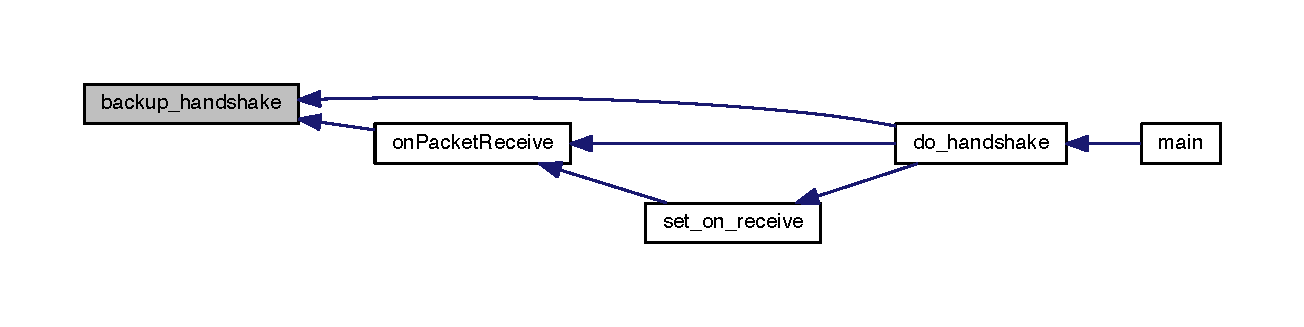
\includegraphics[width=350pt]{_t_l_s_8h_a12a63a5becca8f85a59f6ac0f4d9c553_icgraph}
\end{center}
\end{figure}


\index{T\+L\+S.\+h@{T\+L\+S.\+h}!make\+\_\+certificate@{make\+\_\+certificate}}
\index{make\+\_\+certificate@{make\+\_\+certificate}!T\+L\+S.\+h@{T\+L\+S.\+h}}
\subsubsection[{\texorpdfstring{make\+\_\+certificate(\+T\+L\+S\+\_\+parameters\+\_\+t $\ast$\+T\+L\+S\+\_\+param)}{make_certificate(TLS_parameters_t *TLS_param)}}]{\setlength{\rightskip}{0pt plus 5cm}{\bf handshake\+\_\+t}$\ast$ make\+\_\+certificate (
\begin{DoxyParamCaption}
\item[{{\bf T\+L\+S\+\_\+parameters\+\_\+t} $\ast$}]{T\+L\+S\+\_\+param}
\end{DoxyParamCaption}
)}\hypertarget{_t_l_s_8h_a6fd919275c5d6d3e6578c480cc62a8ce}{}\label{_t_l_s_8h_a6fd919275c5d6d3e6578c480cc62a8ce}
Make the certificate message for the server. That message depends on the authentication algorithm hence we require the connection parameters. The function also sets the certificate in the connection parameters for feature uses.


\begin{DoxyParams}{Parameters}
{\em T\+L\+S\+\_\+param} & \+: connection parameters \\
\hline
\end{DoxyParams}
\begin{DoxyReturn}{Returns}
the certificate handshake message 
\end{DoxyReturn}


Referenced by on\+Packet\+Receive().



Here is the call graph for this function\+:\nopagebreak
\begin{figure}[H]
\begin{center}
\leavevmode
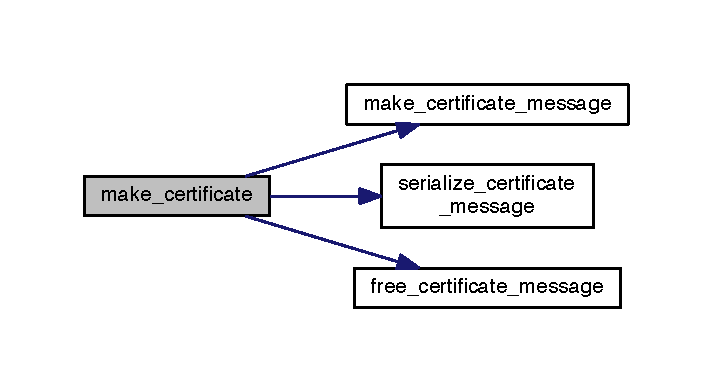
\includegraphics[width=342pt]{_t_l_s_8h_a6fd919275c5d6d3e6578c480cc62a8ce_cgraph}
\end{center}
\end{figure}




Here is the caller graph for this function\+:\nopagebreak
\begin{figure}[H]
\begin{center}
\leavevmode
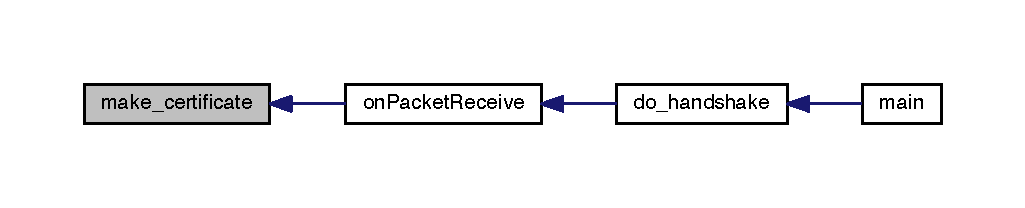
\includegraphics[width=350pt]{_t_l_s_8h_a6fd919275c5d6d3e6578c480cc62a8ce_icgraph}
\end{center}
\end{figure}


\index{T\+L\+S.\+h@{T\+L\+S.\+h}!make\+\_\+change\+\_\+cipher\+\_\+spec@{make\+\_\+change\+\_\+cipher\+\_\+spec}}
\index{make\+\_\+change\+\_\+cipher\+\_\+spec@{make\+\_\+change\+\_\+cipher\+\_\+spec}!T\+L\+S.\+h@{T\+L\+S.\+h}}
\subsubsection[{\texorpdfstring{make\+\_\+change\+\_\+cipher\+\_\+spec()}{make_change_cipher_spec()}}]{\setlength{\rightskip}{0pt plus 5cm}{\bf record\+\_\+t}$\ast$ make\+\_\+change\+\_\+cipher\+\_\+spec (
\begin{DoxyParamCaption}
{}
\end{DoxyParamCaption}
)}\hypertarget{_t_l_s_8h_a5bed323f749e27db36fd6ab2a3e64c4a}{}\label{_t_l_s_8h_a5bed323f749e27db36fd6ab2a3e64c4a}
Make the change cipher spec record message. This message is simple and doesn\textquotesingle{}t require any parameter.

\begin{DoxyReturn}{Returns}
the change cipher spec record 
\end{DoxyReturn}


Referenced by on\+Packet\+Receive().



Here is the caller graph for this function\+:\nopagebreak
\begin{figure}[H]
\begin{center}
\leavevmode
\includegraphics[width=350pt]{_t_l_s_8h_a5bed323f749e27db36fd6ab2a3e64c4a_icgraph}
\end{center}
\end{figure}


\index{T\+L\+S.\+h@{T\+L\+S.\+h}!make\+\_\+client\+\_\+hello@{make\+\_\+client\+\_\+hello}}
\index{make\+\_\+client\+\_\+hello@{make\+\_\+client\+\_\+hello}!T\+L\+S.\+h@{T\+L\+S.\+h}}
\subsubsection[{\texorpdfstring{make\+\_\+client\+\_\+hello(unsigned char $\ast$client\+\_\+random, cipher\+\_\+suite\+\_\+t cipher\+\_\+suite\+\_\+list[], int cipher\+\_\+suite\+\_\+len)}{make_client_hello(unsigned char *client_random, cipher_suite_t cipher_suite_list[], int cipher_suite_len)}}]{\setlength{\rightskip}{0pt plus 5cm}{\bf handshake\+\_\+t}$\ast$ make\+\_\+client\+\_\+hello (
\begin{DoxyParamCaption}
\item[{unsigned char $\ast$}]{client\+\_\+random, }
\item[{{\bf cipher\+\_\+suite\+\_\+t}}]{cipher\+\_\+suite\+\_\+list\mbox{[}$\,$\mbox{]}, }
\item[{int}]{cipher\+\_\+suite\+\_\+len}
\end{DoxyParamCaption}
)}\hypertarget{_t_l_s_8h_a7c6bc0a015a0a78cb508614995b9172e}{}\label{_t_l_s_8h_a7c6bc0a015a0a78cb508614995b9172e}
Given an array of cipher suite make a client hello message. The function also fill the random field using the time stamp and a random generator(openssl)


\begin{DoxyParams}{Parameters}
{\em client\+\_\+random} & \+: the random setted in the client hello \\
\hline
{\em cipher\+\_\+suite\+\_\+list} & \+: an array of cipher suite to add in the client hello \\
\hline
{\em cipher\+\_\+suite\+\_\+len} & \+: the number of cipher suite in the list \\
\hline
\end{DoxyParams}
\begin{DoxyReturn}{Returns}
the hello client handshake message 
\end{DoxyReturn}


Referenced by do\+\_\+handshake().



Here is the call graph for this function\+:\nopagebreak
\begin{figure}[H]
\begin{center}
\leavevmode
\includegraphics[width=330pt]{_t_l_s_8h_a7c6bc0a015a0a78cb508614995b9172e_cgraph}
\end{center}
\end{figure}




Here is the caller graph for this function\+:\nopagebreak
\begin{figure}[H]
\begin{center}
\leavevmode
\includegraphics[width=350pt]{_t_l_s_8h_a7c6bc0a015a0a78cb508614995b9172e_icgraph}
\end{center}
\end{figure}


\index{T\+L\+S.\+h@{T\+L\+S.\+h}!make\+\_\+client\+\_\+key\+\_\+exchange@{make\+\_\+client\+\_\+key\+\_\+exchange}}
\index{make\+\_\+client\+\_\+key\+\_\+exchange@{make\+\_\+client\+\_\+key\+\_\+exchange}!T\+L\+S.\+h@{T\+L\+S.\+h}}
\subsubsection[{\texorpdfstring{make\+\_\+client\+\_\+key\+\_\+exchange(\+T\+L\+S\+\_\+parameters\+\_\+t $\ast$\+T\+L\+S\+\_\+param, uint16\+\_\+t key\+\_\+ex\+\_\+alg)}{make_client_key_exchange(TLS_parameters_t *TLS_param, uint16_t key_ex_alg)}}]{\setlength{\rightskip}{0pt plus 5cm}{\bf handshake\+\_\+t}$\ast$ make\+\_\+client\+\_\+key\+\_\+exchange (
\begin{DoxyParamCaption}
\item[{{\bf T\+L\+S\+\_\+parameters\+\_\+t} $\ast$}]{T\+L\+S\+\_\+param, }
\item[{uint16\+\_\+t}]{key\+\_\+ex\+\_\+alg}
\end{DoxyParamCaption}
)}\hypertarget{_t_l_s_8h_ab3bb4e3f75fb84baa35cd0931381dfe0}{}\label{_t_l_s_8h_ab3bb4e3f75fb84baa35cd0931381dfe0}
Given the information in the T\+L\+S\+\_\+parameter and the key exchange algorithm return the handshake of the client key exchange. That include compute the pre-\/master key. It also compute the master secret and set in the T\+L\+S\+\_\+param.


\begin{DoxyParams}{Parameters}
{\em T\+L\+S\+\_\+param} & \+: the parameters of the connection \\
\hline
{\em key\+\_\+ex\+\_\+alg} & \+: the key exchange algorithm of the handshake \\
\hline
\end{DoxyParams}
\begin{DoxyReturn}{Returns}
the client key exchange handshake message 
\end{DoxyReturn}


Referenced by on\+Packet\+Receive().



Here is the call graph for this function\+:\nopagebreak
\begin{figure}[H]
\begin{center}
\leavevmode
\includegraphics[width=350pt]{_t_l_s_8h_ab3bb4e3f75fb84baa35cd0931381dfe0_cgraph}
\end{center}
\end{figure}




Here is the caller graph for this function\+:\nopagebreak
\begin{figure}[H]
\begin{center}
\leavevmode
\includegraphics[width=350pt]{_t_l_s_8h_ab3bb4e3f75fb84baa35cd0931381dfe0_icgraph}
\end{center}
\end{figure}


\index{T\+L\+S.\+h@{T\+L\+S.\+h}!make\+\_\+finished\+\_\+message@{make\+\_\+finished\+\_\+message}}
\index{make\+\_\+finished\+\_\+message@{make\+\_\+finished\+\_\+message}!T\+L\+S.\+h@{T\+L\+S.\+h}}
\subsubsection[{\texorpdfstring{make\+\_\+finished\+\_\+message(\+T\+L\+S\+\_\+parameters\+\_\+t $\ast$\+T\+L\+S\+\_\+param)}{make_finished_message(TLS_parameters_t *TLS_param)}}]{\setlength{\rightskip}{0pt plus 5cm}{\bf handshake\+\_\+t}$\ast$ make\+\_\+finished\+\_\+message (
\begin{DoxyParamCaption}
\item[{{\bf T\+L\+S\+\_\+parameters\+\_\+t} $\ast$}]{T\+L\+S\+\_\+param}
\end{DoxyParamCaption}
)}\hypertarget{_t_l_s_8h_ae149244e09cbbd2180bc4c5fc6d0a924}{}\label{_t_l_s_8h_ae149244e09cbbd2180bc4c5fc6d0a924}
Given the connection parameters compute the finished message. Note in the T\+LS protocol this message is encrypted.


\begin{DoxyParams}{Parameters}
{\em T\+L\+S\+\_\+param} & \+: the connection parameters \\
\hline
\end{DoxyParams}
\begin{DoxyReturn}{Returns}
the finished handshake message 
\end{DoxyReturn}


Referenced by on\+Packet\+Receive().



Here is the call graph for this function\+:\nopagebreak
\begin{figure}[H]
\begin{center}
\leavevmode
\includegraphics[width=342pt]{_t_l_s_8h_ae149244e09cbbd2180bc4c5fc6d0a924_cgraph}
\end{center}
\end{figure}




Here is the caller graph for this function\+:\nopagebreak
\begin{figure}[H]
\begin{center}
\leavevmode
\includegraphics[width=350pt]{_t_l_s_8h_ae149244e09cbbd2180bc4c5fc6d0a924_icgraph}
\end{center}
\end{figure}


\index{T\+L\+S.\+h@{T\+L\+S.\+h}!make\+\_\+server\+\_\+hello@{make\+\_\+server\+\_\+hello}}
\index{make\+\_\+server\+\_\+hello@{make\+\_\+server\+\_\+hello}!T\+L\+S.\+h@{T\+L\+S.\+h}}
\subsubsection[{\texorpdfstring{make\+\_\+server\+\_\+hello(\+T\+L\+S\+\_\+parameters\+\_\+t $\ast$\+T\+L\+S\+\_\+param, server\+\_\+client\+\_\+hello\+\_\+t $\ast$client\+\_\+hello)}{make_server_hello(TLS_parameters_t *TLS_param, server_client_hello_t *client_hello)}}]{\setlength{\rightskip}{0pt plus 5cm}{\bf handshake\+\_\+t}$\ast$ make\+\_\+server\+\_\+hello (
\begin{DoxyParamCaption}
\item[{{\bf T\+L\+S\+\_\+parameters\+\_\+t} $\ast$}]{T\+L\+S\+\_\+param, }
\item[{{\bf server\+\_\+client\+\_\+hello\+\_\+t} $\ast$}]{client\+\_\+hello}
\end{DoxyParamCaption}
)}\hypertarget{_t_l_s_8h_a035a830fd89c6c7af60809197d81ea29}{}\label{_t_l_s_8h_a035a830fd89c6c7af60809197d81ea29}
Given the client hello message the function makes the server hello. It choices a random cipher suite among the those provided by the client. The function also fill the random field using the time stamp and a random generator(openssl)


\begin{DoxyParams}{Parameters}
{\em T\+L\+S\+\_\+param} & \+: the connection parameters \\
\hline
{\em client\+\_\+hello} & \+: the received client hello. \\
\hline
\end{DoxyParams}
\begin{DoxyReturn}{Returns}
the hello server handshake message 
\end{DoxyReturn}


Referenced by on\+Packet\+Receive().



Here is the call graph for this function\+:\nopagebreak
\begin{figure}[H]
\begin{center}
\leavevmode
\includegraphics[width=338pt]{_t_l_s_8h_a035a830fd89c6c7af60809197d81ea29_cgraph}
\end{center}
\end{figure}




Here is the caller graph for this function\+:\nopagebreak
\begin{figure}[H]
\begin{center}
\leavevmode
\includegraphics[width=350pt]{_t_l_s_8h_a035a830fd89c6c7af60809197d81ea29_icgraph}
\end{center}
\end{figure}


\index{T\+L\+S.\+h@{T\+L\+S.\+h}!make\+\_\+server\+\_\+hello\+\_\+done@{make\+\_\+server\+\_\+hello\+\_\+done}}
\index{make\+\_\+server\+\_\+hello\+\_\+done@{make\+\_\+server\+\_\+hello\+\_\+done}!T\+L\+S.\+h@{T\+L\+S.\+h}}
\subsubsection[{\texorpdfstring{make\+\_\+server\+\_\+hello\+\_\+done()}{make_server_hello_done()}}]{\setlength{\rightskip}{0pt plus 5cm}{\bf handshake\+\_\+t}$\ast$ make\+\_\+server\+\_\+hello\+\_\+done (
\begin{DoxyParamCaption}
{}
\end{DoxyParamCaption}
)}\hypertarget{_t_l_s_8h_af98aa49e2563d588c366ef1712de925a}{}\label{_t_l_s_8h_af98aa49e2563d588c366ef1712de925a}
Make the server hello done message. This message is simple and doesn\textquotesingle{}t require any parameter.

\begin{DoxyReturn}{Returns}
the server hello done handshake message 
\end{DoxyReturn}


Referenced by on\+Packet\+Receive().



Here is the caller graph for this function\+:\nopagebreak
\begin{figure}[H]
\begin{center}
\leavevmode
\includegraphics[width=350pt]{_t_l_s_8h_af98aa49e2563d588c366ef1712de925a_icgraph}
\end{center}
\end{figure}


\index{T\+L\+S.\+h@{T\+L\+S.\+h}!make\+\_\+server\+\_\+key\+\_\+exchange@{make\+\_\+server\+\_\+key\+\_\+exchange}}
\index{make\+\_\+server\+\_\+key\+\_\+exchange@{make\+\_\+server\+\_\+key\+\_\+exchange}!T\+L\+S.\+h@{T\+L\+S.\+h}}
\subsubsection[{\texorpdfstring{make\+\_\+server\+\_\+key\+\_\+exchange(\+T\+L\+S\+\_\+parameters\+\_\+t $\ast$\+T\+L\+S\+\_\+param)}{make_server_key_exchange(TLS_parameters_t *TLS_param)}}]{\setlength{\rightskip}{0pt plus 5cm}{\bf handshake\+\_\+t}$\ast$ make\+\_\+server\+\_\+key\+\_\+exchange (
\begin{DoxyParamCaption}
\item[{{\bf T\+L\+S\+\_\+parameters\+\_\+t} $\ast$}]{T\+L\+S\+\_\+param}
\end{DoxyParamCaption}
)}\hypertarget{_t_l_s_8h_a902d940508d7080023ef072b2667a143}{}\label{_t_l_s_8h_a902d940508d7080023ef072b2667a143}
Make the server key exchange handshake message. The function also sets the message in the connection parameters for compute the master key in the client key exchange message.


\begin{DoxyParams}{Parameters}
{\em T\+L\+S\+\_\+param} & \+: connection parameters \\
\hline
\end{DoxyParams}
\begin{DoxyReturn}{Returns}
the server key exchange handshake message 
\end{DoxyReturn}


Referenced by on\+Packet\+Receive().



Here is the call graph for this function\+:\nopagebreak
\begin{figure}[H]
\begin{center}
\leavevmode
\includegraphics[width=350pt]{_t_l_s_8h_a902d940508d7080023ef072b2667a143_cgraph}
\end{center}
\end{figure}




Here is the caller graph for this function\+:\nopagebreak
\begin{figure}[H]
\begin{center}
\leavevmode
\includegraphics[width=350pt]{_t_l_s_8h_a902d940508d7080023ef072b2667a143_icgraph}
\end{center}
\end{figure}



\hypertarget{_t_l_s_constants_8h}{}\section{include/\+T\+L\+S\+Constants.h File Reference}
\label{_t_l_s_constants_8h}\index{include/\+T\+L\+S\+Constants.\+h@{include/\+T\+L\+S\+Constants.\+h}}
{\ttfamily \#include $<$stdio.\+h$>$}\\*
{\ttfamily \#include $<$stdint.\+h$>$}\\*
{\ttfamily \#include $<$string.\+h$>$}\\*
{\ttfamily \#include $<$openssl/hmac.\+h$>$}\\*
Include dependency graph for T\+L\+S\+Constants.\+h\+:
\nopagebreak
\begin{figure}[H]
\begin{center}
\leavevmode
\includegraphics[width=350pt]{_t_l_s_constants_8h__incl}
\end{center}
\end{figure}
This graph shows which files directly or indirectly include this file\+:
\nopagebreak
\begin{figure}[H]
\begin{center}
\leavevmode
\includegraphics[width=350pt]{_t_l_s_constants_8h__dep__incl}
\end{center}
\end{figure}
\subsection*{Data Structures}
\begin{DoxyCompactItemize}
\item 
struct \hyperlink{structcipher__suite__t}{cipher\+\_\+suite\+\_\+t}
\end{DoxyCompactItemize}
\subsection*{Macros}
\begin{DoxyCompactItemize}
\item 
\#define \hyperlink{_t_l_s_constants_8h_ab7690321561c4c2f8e301abd41440aa4}{R\+E\+V16}(value)~(\{(value \& 0x00\+F\+F\+U) $<$$<$ 8 $\vert$ (value \& 0x\+F\+F00\+U) $>$$>$ 8;\})
\item 
\#define \hyperlink{_t_l_s_constants_8h_aac89d13e711b8a32822746e51237265c}{R\+E\+V32}(value)~(\{(value \& 0x000000\+F\+F\+U) $<$$<$ 24 $\vert$ (value \& 0x0000\+F\+F00\+U) $<$$<$ 8 $\vert$(value \& 0x00\+F\+F0000\+U) $>$$>$ 8 $\vert$ (value \& 0x\+F\+F000000\+U) $>$$>$ 24;\})
\end{DoxyCompactItemize}
\subsection*{Enumerations}
\subsection*{Functions}
\begin{DoxyCompactItemize}
\item 
const E\+V\+P\+\_\+\+MD $\ast$ \hyperlink{_t_l_s_constants_8h_a98e6374e1aa179c023ba0eb8bdf36196}{get\+\_\+hash\+\_\+function} (\hyperlink{_t_l_s_constants_8h_a0f89141ac474c59cb87d2eb5e16a598f}{hash\+\_\+algorithm} h)
\item 
\hyperlink{structcipher__suite__t}{cipher\+\_\+suite\+\_\+t} \hyperlink{_t_l_s_constants_8h_a7f66c07120c851032c213bdadcff2009}{get\+\_\+cipher\+\_\+suite\+\_\+by\+\_\+id} (uint16\+\_\+t id)
\item 
\hyperlink{structcipher__suite__t}{cipher\+\_\+suite\+\_\+t} \hyperlink{_t_l_s_constants_8h_abdfed4eb10938d5d14bc8a37f1f8d950}{get\+\_\+cipher\+\_\+suite\+\_\+by\+\_\+name} (char $\ast$name)
\item 
int \hyperlink{_t_l_s_constants_8h_ae63f6745a9c92927fc9d574d40262ac3}{get\+\_\+cipher\+\_\+suites} (\hyperlink{_t_l_s_constants_8h_a7203e83530e35d8ed2f3300ba0408a54}{key\+\_\+exchange\+\_\+algorithm} kx, \hyperlink{_t_l_s_constants_8h_a0f89141ac474c59cb87d2eb5e16a598f}{hash\+\_\+algorithm} h, \hyperlink{_t_l_s_constants_8h_a433e2522c8a62ae4d8b1c91badefef50}{authentication\+\_\+algorithm} au, \hyperlink{structcipher__suite__t}{cipher\+\_\+suite\+\_\+t} array\mbox{[}$\,$\mbox{]})
\end{DoxyCompactItemize}
\subsection*{Variables}
\begin{DoxyCompactItemize}
\item 
const int \hyperlink{_t_l_s_constants_8h_a9dabc5b9445bb0547de6bec83d9cdc3e}{N\+U\+M\+\_\+\+C\+I\+P\+H\+E\+R\+\_\+\+S\+U\+I\+TE}
\end{DoxyCompactItemize}


\subsection{Detailed Description}
S\+S\+L/\+T\+LS Project

This file contains a set of constants used in the handshake protocol and function interface for manage the supported cipher suite.

\begin{DoxyDate}{Date}
Created on 24/12/15. 
\end{DoxyDate}
\begin{DoxyCopyright}{Copyright}
Copyright © 2015 Alessandro Melloni, Andrea Francesco Vinci. All rights reserved. 
\end{DoxyCopyright}


\subsection{Macro Definition Documentation}
\index{T\+L\+S\+Constants.\+h@{T\+L\+S\+Constants.\+h}!R\+E\+V16@{R\+E\+V16}}
\index{R\+E\+V16@{R\+E\+V16}!T\+L\+S\+Constants.\+h@{T\+L\+S\+Constants.\+h}}
\subsubsection[{\texorpdfstring{R\+E\+V16}{REV16}}]{\setlength{\rightskip}{0pt plus 5cm}\#define R\+E\+V16(
\begin{DoxyParamCaption}
\item[{}]{value}
\end{DoxyParamCaption}
)~(\{(value \& 0x00\+F\+F\+U) $<$$<$ 8 $\vert$ (value \& 0x\+F\+F00\+U) $>$$>$ 8;\})}\hypertarget{_t_l_s_constants_8h_ab7690321561c4c2f8e301abd41440aa4}{}\label{_t_l_s_constants_8h_ab7690321561c4c2f8e301abd41440aa4}
Rotational byte for uint16 \index{T\+L\+S\+Constants.\+h@{T\+L\+S\+Constants.\+h}!R\+E\+V32@{R\+E\+V32}}
\index{R\+E\+V32@{R\+E\+V32}!T\+L\+S\+Constants.\+h@{T\+L\+S\+Constants.\+h}}
\subsubsection[{\texorpdfstring{R\+E\+V32}{REV32}}]{\setlength{\rightskip}{0pt plus 5cm}\#define R\+E\+V32(
\begin{DoxyParamCaption}
\item[{}]{value}
\end{DoxyParamCaption}
)~(\{(value \& 0x000000\+F\+F\+U) $<$$<$ 24 $\vert$ (value \& 0x0000\+F\+F00\+U) $<$$<$ 8 $\vert$(value \& 0x00\+F\+F0000\+U) $>$$>$ 8 $\vert$ (value \& 0x\+F\+F000000\+U) $>$$>$ 24;\})}\hypertarget{_t_l_s_constants_8h_aac89d13e711b8a32822746e51237265c}{}\label{_t_l_s_constants_8h_aac89d13e711b8a32822746e51237265c}
Rotational byte for uint32 

Referenced by deserialize\+\_\+certificate\+\_\+message(), deserialize\+\_\+client\+\_\+server\+\_\+hello(), deserialize\+\_\+handshake(), serialize\+\_\+certificate\+\_\+message(), serialize\+\_\+client\+\_\+server\+\_\+hello(), and serialize\+\_\+handshake().



\subsection{Enumeration Type Documentation}
\subsubsection[{\texorpdfstring{anonymous enum}{anonymous enum}}]{\setlength{\rightskip}{0pt plus 5cm}anonymous enum}\hypertarget{_t_l_s_constants_8h_a06fc87d81c62e9abb8790b6e5713c55b}{}\label{_t_l_s_constants_8h_a06fc87d81c62e9abb8790b6e5713c55b}
\begin{Desc}
\item[Enumerator]\par
\begin{description}
\index{H\+E\+L\+L\+O\+\_\+\+R\+E\+Q\+U\+E\+ST@{H\+E\+L\+L\+O\+\_\+\+R\+E\+Q\+U\+E\+ST}!T\+L\+S\+Constants.\+h@{T\+L\+S\+Constants.\+h}}\index{T\+L\+S\+Constants.\+h@{T\+L\+S\+Constants.\+h}!H\+E\+L\+L\+O\+\_\+\+R\+E\+Q\+U\+E\+ST@{H\+E\+L\+L\+O\+\_\+\+R\+E\+Q\+U\+E\+ST}}\item[{\em 
H\+E\+L\+L\+O\+\_\+\+R\+E\+Q\+U\+E\+ST\hypertarget{_t_l_s_constants_8h_a06fc87d81c62e9abb8790b6e5713c55babae9b7a6a527c720a4eab46d35a4ed71}{}\label{_t_l_s_constants_8h_a06fc87d81c62e9abb8790b6e5713c55babae9b7a6a527c720a4eab46d35a4ed71}
}]\index{C\+L\+I\+E\+N\+T\+\_\+\+H\+E\+L\+LO@{C\+L\+I\+E\+N\+T\+\_\+\+H\+E\+L\+LO}!T\+L\+S\+Constants.\+h@{T\+L\+S\+Constants.\+h}}\index{T\+L\+S\+Constants.\+h@{T\+L\+S\+Constants.\+h}!C\+L\+I\+E\+N\+T\+\_\+\+H\+E\+L\+LO@{C\+L\+I\+E\+N\+T\+\_\+\+H\+E\+L\+LO}}\item[{\em 
C\+L\+I\+E\+N\+T\+\_\+\+H\+E\+L\+LO\hypertarget{_t_l_s_constants_8h_a06fc87d81c62e9abb8790b6e5713c55ba0c8da6c451065bed79ea70684e6f3fca}{}\label{_t_l_s_constants_8h_a06fc87d81c62e9abb8790b6e5713c55ba0c8da6c451065bed79ea70684e6f3fca}
}]\index{S\+E\+R\+V\+E\+R\+\_\+\+H\+E\+L\+LO@{S\+E\+R\+V\+E\+R\+\_\+\+H\+E\+L\+LO}!T\+L\+S\+Constants.\+h@{T\+L\+S\+Constants.\+h}}\index{T\+L\+S\+Constants.\+h@{T\+L\+S\+Constants.\+h}!S\+E\+R\+V\+E\+R\+\_\+\+H\+E\+L\+LO@{S\+E\+R\+V\+E\+R\+\_\+\+H\+E\+L\+LO}}\item[{\em 
S\+E\+R\+V\+E\+R\+\_\+\+H\+E\+L\+LO\hypertarget{_t_l_s_constants_8h_a06fc87d81c62e9abb8790b6e5713c55ba28914d3bb26ec8c2bd2d5ad9781cbf8c}{}\label{_t_l_s_constants_8h_a06fc87d81c62e9abb8790b6e5713c55ba28914d3bb26ec8c2bd2d5ad9781cbf8c}
}]\index{C\+E\+R\+T\+I\+F\+I\+C\+A\+TE@{C\+E\+R\+T\+I\+F\+I\+C\+A\+TE}!T\+L\+S\+Constants.\+h@{T\+L\+S\+Constants.\+h}}\index{T\+L\+S\+Constants.\+h@{T\+L\+S\+Constants.\+h}!C\+E\+R\+T\+I\+F\+I\+C\+A\+TE@{C\+E\+R\+T\+I\+F\+I\+C\+A\+TE}}\item[{\em 
C\+E\+R\+T\+I\+F\+I\+C\+A\+TE\hypertarget{_t_l_s_constants_8h_a06fc87d81c62e9abb8790b6e5713c55baaf428ae486a42ccf4119898f179e3a07}{}\label{_t_l_s_constants_8h_a06fc87d81c62e9abb8790b6e5713c55baaf428ae486a42ccf4119898f179e3a07}
}]\index{S\+E\+R\+V\+E\+R\+\_\+\+K\+E\+Y\+\_\+\+E\+X\+C\+H\+A\+N\+GE@{S\+E\+R\+V\+E\+R\+\_\+\+K\+E\+Y\+\_\+\+E\+X\+C\+H\+A\+N\+GE}!T\+L\+S\+Constants.\+h@{T\+L\+S\+Constants.\+h}}\index{T\+L\+S\+Constants.\+h@{T\+L\+S\+Constants.\+h}!S\+E\+R\+V\+E\+R\+\_\+\+K\+E\+Y\+\_\+\+E\+X\+C\+H\+A\+N\+GE@{S\+E\+R\+V\+E\+R\+\_\+\+K\+E\+Y\+\_\+\+E\+X\+C\+H\+A\+N\+GE}}\item[{\em 
S\+E\+R\+V\+E\+R\+\_\+\+K\+E\+Y\+\_\+\+E\+X\+C\+H\+A\+N\+GE\hypertarget{_t_l_s_constants_8h_a06fc87d81c62e9abb8790b6e5713c55babe276092f7af8dc33c7b4de9f51cd607}{}\label{_t_l_s_constants_8h_a06fc87d81c62e9abb8790b6e5713c55babe276092f7af8dc33c7b4de9f51cd607}
}]\index{C\+E\+R\+T\+I\+F\+I\+C\+A\+T\+E\+\_\+\+R\+E\+Q\+U\+E\+ST@{C\+E\+R\+T\+I\+F\+I\+C\+A\+T\+E\+\_\+\+R\+E\+Q\+U\+E\+ST}!T\+L\+S\+Constants.\+h@{T\+L\+S\+Constants.\+h}}\index{T\+L\+S\+Constants.\+h@{T\+L\+S\+Constants.\+h}!C\+E\+R\+T\+I\+F\+I\+C\+A\+T\+E\+\_\+\+R\+E\+Q\+U\+E\+ST@{C\+E\+R\+T\+I\+F\+I\+C\+A\+T\+E\+\_\+\+R\+E\+Q\+U\+E\+ST}}\item[{\em 
C\+E\+R\+T\+I\+F\+I\+C\+A\+T\+E\+\_\+\+R\+E\+Q\+U\+E\+ST\hypertarget{_t_l_s_constants_8h_a06fc87d81c62e9abb8790b6e5713c55ba0defc0af2846f90d1786d817a7af5516}{}\label{_t_l_s_constants_8h_a06fc87d81c62e9abb8790b6e5713c55ba0defc0af2846f90d1786d817a7af5516}
}]\index{S\+E\+R\+V\+E\+R\+\_\+\+D\+O\+NE@{S\+E\+R\+V\+E\+R\+\_\+\+D\+O\+NE}!T\+L\+S\+Constants.\+h@{T\+L\+S\+Constants.\+h}}\index{T\+L\+S\+Constants.\+h@{T\+L\+S\+Constants.\+h}!S\+E\+R\+V\+E\+R\+\_\+\+D\+O\+NE@{S\+E\+R\+V\+E\+R\+\_\+\+D\+O\+NE}}\item[{\em 
S\+E\+R\+V\+E\+R\+\_\+\+D\+O\+NE\hypertarget{_t_l_s_constants_8h_a06fc87d81c62e9abb8790b6e5713c55baa7a5264dd122628f26d55e601a05bcf1}{}\label{_t_l_s_constants_8h_a06fc87d81c62e9abb8790b6e5713c55baa7a5264dd122628f26d55e601a05bcf1}
}]\index{C\+E\+R\+T\+I\+F\+I\+C\+A\+T\+E\+\_\+\+V\+E\+R\+I\+FY@{C\+E\+R\+T\+I\+F\+I\+C\+A\+T\+E\+\_\+\+V\+E\+R\+I\+FY}!T\+L\+S\+Constants.\+h@{T\+L\+S\+Constants.\+h}}\index{T\+L\+S\+Constants.\+h@{T\+L\+S\+Constants.\+h}!C\+E\+R\+T\+I\+F\+I\+C\+A\+T\+E\+\_\+\+V\+E\+R\+I\+FY@{C\+E\+R\+T\+I\+F\+I\+C\+A\+T\+E\+\_\+\+V\+E\+R\+I\+FY}}\item[{\em 
C\+E\+R\+T\+I\+F\+I\+C\+A\+T\+E\+\_\+\+V\+E\+R\+I\+FY\hypertarget{_t_l_s_constants_8h_a06fc87d81c62e9abb8790b6e5713c55ba1e6ed3d0ebef1c53bf791791547bf475}{}\label{_t_l_s_constants_8h_a06fc87d81c62e9abb8790b6e5713c55ba1e6ed3d0ebef1c53bf791791547bf475}
}]\index{C\+L\+I\+E\+N\+T\+\_\+\+K\+E\+Y\+\_\+\+E\+X\+C\+H\+A\+N\+GE@{C\+L\+I\+E\+N\+T\+\_\+\+K\+E\+Y\+\_\+\+E\+X\+C\+H\+A\+N\+GE}!T\+L\+S\+Constants.\+h@{T\+L\+S\+Constants.\+h}}\index{T\+L\+S\+Constants.\+h@{T\+L\+S\+Constants.\+h}!C\+L\+I\+E\+N\+T\+\_\+\+K\+E\+Y\+\_\+\+E\+X\+C\+H\+A\+N\+GE@{C\+L\+I\+E\+N\+T\+\_\+\+K\+E\+Y\+\_\+\+E\+X\+C\+H\+A\+N\+GE}}\item[{\em 
C\+L\+I\+E\+N\+T\+\_\+\+K\+E\+Y\+\_\+\+E\+X\+C\+H\+A\+N\+GE\hypertarget{_t_l_s_constants_8h_a06fc87d81c62e9abb8790b6e5713c55ba2fcb8d386327535a875365fc4638cc47}{}\label{_t_l_s_constants_8h_a06fc87d81c62e9abb8790b6e5713c55ba2fcb8d386327535a875365fc4638cc47}
}]\index{F\+I\+N\+I\+S\+H\+ED@{F\+I\+N\+I\+S\+H\+ED}!T\+L\+S\+Constants.\+h@{T\+L\+S\+Constants.\+h}}\index{T\+L\+S\+Constants.\+h@{T\+L\+S\+Constants.\+h}!F\+I\+N\+I\+S\+H\+ED@{F\+I\+N\+I\+S\+H\+ED}}\item[{\em 
F\+I\+N\+I\+S\+H\+ED\hypertarget{_t_l_s_constants_8h_a06fc87d81c62e9abb8790b6e5713c55badbd1812bee789fbf3548cf79d3f2b400}{}\label{_t_l_s_constants_8h_a06fc87d81c62e9abb8790b6e5713c55badbd1812bee789fbf3548cf79d3f2b400}
}]\end{description}
\end{Desc}
\index{T\+L\+S\+Constants.\+h@{T\+L\+S\+Constants.\+h}!authentication\+\_\+algorithm@{authentication\+\_\+algorithm}}
\index{authentication\+\_\+algorithm@{authentication\+\_\+algorithm}!T\+L\+S\+Constants.\+h@{T\+L\+S\+Constants.\+h}}
\subsubsection[{\texorpdfstring{authentication\+\_\+algorithm}{authentication_algorithm}}]{\setlength{\rightskip}{0pt plus 5cm}enum {\bf authentication\+\_\+algorithm}}\hypertarget{_t_l_s_constants_8h_a433e2522c8a62ae4d8b1c91badefef50}{}\label{_t_l_s_constants_8h_a433e2522c8a62ae4d8b1c91badefef50}
Different type of authentication algorithm \begin{Desc}
\item[Enumerator]\par
\begin{description}
\index{N\+O\+N\+E\+\_\+\+AU@{N\+O\+N\+E\+\_\+\+AU}!T\+L\+S\+Constants.\+h@{T\+L\+S\+Constants.\+h}}\index{T\+L\+S\+Constants.\+h@{T\+L\+S\+Constants.\+h}!N\+O\+N\+E\+\_\+\+AU@{N\+O\+N\+E\+\_\+\+AU}}\item[{\em 
N\+O\+N\+E\+\_\+\+AU\hypertarget{_t_l_s_constants_8h_a433e2522c8a62ae4d8b1c91badefef50a964e2fcfb3e662df2720a32d28538a6a}{}\label{_t_l_s_constants_8h_a433e2522c8a62ae4d8b1c91badefef50a964e2fcfb3e662df2720a32d28538a6a}
}]No algorithm \index{R\+S\+A\+\_\+\+AU@{R\+S\+A\+\_\+\+AU}!T\+L\+S\+Constants.\+h@{T\+L\+S\+Constants.\+h}}\index{T\+L\+S\+Constants.\+h@{T\+L\+S\+Constants.\+h}!R\+S\+A\+\_\+\+AU@{R\+S\+A\+\_\+\+AU}}\item[{\em 
R\+S\+A\+\_\+\+AU\hypertarget{_t_l_s_constants_8h_a433e2522c8a62ae4d8b1c91badefef50a89f44b27b8e2464a498e4ba3f8fc22fc}{}\label{_t_l_s_constants_8h_a433e2522c8a62ae4d8b1c91badefef50a89f44b27b8e2464a498e4ba3f8fc22fc}
}]R\+SA signature \index{D\+S\+S\+\_\+\+AU@{D\+S\+S\+\_\+\+AU}!T\+L\+S\+Constants.\+h@{T\+L\+S\+Constants.\+h}}\index{T\+L\+S\+Constants.\+h@{T\+L\+S\+Constants.\+h}!D\+S\+S\+\_\+\+AU@{D\+S\+S\+\_\+\+AU}}\item[{\em 
D\+S\+S\+\_\+\+AU\hypertarget{_t_l_s_constants_8h_a433e2522c8a62ae4d8b1c91badefef50ad2bfec02f0c8b7252dee8e58eb1f9904}{}\label{_t_l_s_constants_8h_a433e2522c8a62ae4d8b1c91badefef50ad2bfec02f0c8b7252dee8e58eb1f9904}
}]D\+SA signature \index{E\+C\+D\+S\+A\+\_\+\+AU@{E\+C\+D\+S\+A\+\_\+\+AU}!T\+L\+S\+Constants.\+h@{T\+L\+S\+Constants.\+h}}\index{T\+L\+S\+Constants.\+h@{T\+L\+S\+Constants.\+h}!E\+C\+D\+S\+A\+\_\+\+AU@{E\+C\+D\+S\+A\+\_\+\+AU}}\item[{\em 
E\+C\+D\+S\+A\+\_\+\+AU\hypertarget{_t_l_s_constants_8h_a433e2522c8a62ae4d8b1c91badefef50a83b74be0583f5ebc8fb148a73f1f2af8}{}\label{_t_l_s_constants_8h_a433e2522c8a62ae4d8b1c91badefef50a83b74be0583f5ebc8fb148a73f1f2af8}
}]E\+C\+D\+SA signature \end{description}
\end{Desc}
\index{T\+L\+S\+Constants.\+h@{T\+L\+S\+Constants.\+h}!channel\+\_\+mode@{channel\+\_\+mode}}
\index{channel\+\_\+mode@{channel\+\_\+mode}!T\+L\+S\+Constants.\+h@{T\+L\+S\+Constants.\+h}}
\subsubsection[{\texorpdfstring{channel\+\_\+mode}{channel_mode}}]{\setlength{\rightskip}{0pt plus 5cm}enum {\bf channel\+\_\+mode}}\hypertarget{_t_l_s_constants_8h_af21001704588d21e61c566facf69ec3d}{}\label{_t_l_s_constants_8h_af21001704588d21e61c566facf69ec3d}
Enum used for set the packet mode e.\+g. server\+\_\+hello, client\+\_\+hello \begin{Desc}
\item[Enumerator]\par
\begin{description}
\index{S\+E\+R\+V\+E\+R\+\_\+\+M\+O\+DE@{S\+E\+R\+V\+E\+R\+\_\+\+M\+O\+DE}!T\+L\+S\+Constants.\+h@{T\+L\+S\+Constants.\+h}}\index{T\+L\+S\+Constants.\+h@{T\+L\+S\+Constants.\+h}!S\+E\+R\+V\+E\+R\+\_\+\+M\+O\+DE@{S\+E\+R\+V\+E\+R\+\_\+\+M\+O\+DE}}\item[{\em 
S\+E\+R\+V\+E\+R\+\_\+\+M\+O\+DE\hypertarget{_t_l_s_constants_8h_af21001704588d21e61c566facf69ec3daa93134a3bb4b74bc01af0b16d0621035}{}\label{_t_l_s_constants_8h_af21001704588d21e61c566facf69ec3daa93134a3bb4b74bc01af0b16d0621035}
}]\index{C\+L\+I\+E\+N\+T\+\_\+\+M\+O\+DE@{C\+L\+I\+E\+N\+T\+\_\+\+M\+O\+DE}!T\+L\+S\+Constants.\+h@{T\+L\+S\+Constants.\+h}}\index{T\+L\+S\+Constants.\+h@{T\+L\+S\+Constants.\+h}!C\+L\+I\+E\+N\+T\+\_\+\+M\+O\+DE@{C\+L\+I\+E\+N\+T\+\_\+\+M\+O\+DE}}\item[{\em 
C\+L\+I\+E\+N\+T\+\_\+\+M\+O\+DE\hypertarget{_t_l_s_constants_8h_af21001704588d21e61c566facf69ec3da7aba1b408dc6d2d1b01b58a09893f204}{}\label{_t_l_s_constants_8h_af21001704588d21e61c566facf69ec3da7aba1b408dc6d2d1b01b58a09893f204}
}]\end{description}
\end{Desc}
\index{T\+L\+S\+Constants.\+h@{T\+L\+S\+Constants.\+h}!hash\+\_\+algorithm@{hash\+\_\+algorithm}}
\index{hash\+\_\+algorithm@{hash\+\_\+algorithm}!T\+L\+S\+Constants.\+h@{T\+L\+S\+Constants.\+h}}
\subsubsection[{\texorpdfstring{hash\+\_\+algorithm}{hash_algorithm}}]{\setlength{\rightskip}{0pt plus 5cm}enum {\bf hash\+\_\+algorithm}}\hypertarget{_t_l_s_constants_8h_a0f89141ac474c59cb87d2eb5e16a598f}{}\label{_t_l_s_constants_8h_a0f89141ac474c59cb87d2eb5e16a598f}
Different type of hash algorithm \begin{Desc}
\item[Enumerator]\par
\begin{description}
\index{N\+O\+N\+E\+\_\+H@{N\+O\+N\+E\+\_\+H}!T\+L\+S\+Constants.\+h@{T\+L\+S\+Constants.\+h}}\index{T\+L\+S\+Constants.\+h@{T\+L\+S\+Constants.\+h}!N\+O\+N\+E\+\_\+H@{N\+O\+N\+E\+\_\+H}}\item[{\em 
N\+O\+N\+E\+\_\+H\hypertarget{_t_l_s_constants_8h_a0f89141ac474c59cb87d2eb5e16a598fa49c07755882c1f42cc85203661d56a54}{}\label{_t_l_s_constants_8h_a0f89141ac474c59cb87d2eb5e16a598fa49c07755882c1f42cc85203661d56a54}
}]No hash \index{M\+D5\+\_\+H@{M\+D5\+\_\+H}!T\+L\+S\+Constants.\+h@{T\+L\+S\+Constants.\+h}}\index{T\+L\+S\+Constants.\+h@{T\+L\+S\+Constants.\+h}!M\+D5\+\_\+H@{M\+D5\+\_\+H}}\item[{\em 
M\+D5\+\_\+H\hypertarget{_t_l_s_constants_8h_a0f89141ac474c59cb87d2eb5e16a598fa3d5dd00a9e85fda90862297578ecb61f}{}\label{_t_l_s_constants_8h_a0f89141ac474c59cb87d2eb5e16a598fa3d5dd00a9e85fda90862297578ecb61f}
}]M\+D5 \index{S\+H\+A1\+\_\+H@{S\+H\+A1\+\_\+H}!T\+L\+S\+Constants.\+h@{T\+L\+S\+Constants.\+h}}\index{T\+L\+S\+Constants.\+h@{T\+L\+S\+Constants.\+h}!S\+H\+A1\+\_\+H@{S\+H\+A1\+\_\+H}}\item[{\em 
S\+H\+A1\+\_\+H\hypertarget{_t_l_s_constants_8h_a0f89141ac474c59cb87d2eb5e16a598fa79b80ad65c6aec14c648ddb9498e2fe2}{}\label{_t_l_s_constants_8h_a0f89141ac474c59cb87d2eb5e16a598fa79b80ad65c6aec14c648ddb9498e2fe2}
}]S\+HA 1 \index{S\+H\+A224\+\_\+H@{S\+H\+A224\+\_\+H}!T\+L\+S\+Constants.\+h@{T\+L\+S\+Constants.\+h}}\index{T\+L\+S\+Constants.\+h@{T\+L\+S\+Constants.\+h}!S\+H\+A224\+\_\+H@{S\+H\+A224\+\_\+H}}\item[{\em 
S\+H\+A224\+\_\+H\hypertarget{_t_l_s_constants_8h_a0f89141ac474c59cb87d2eb5e16a598faf48cc96dc4109fad452f92d9a28fef27}{}\label{_t_l_s_constants_8h_a0f89141ac474c59cb87d2eb5e16a598faf48cc96dc4109fad452f92d9a28fef27}
}]S\+HA 224 \index{S\+H\+A256\+\_\+H@{S\+H\+A256\+\_\+H}!T\+L\+S\+Constants.\+h@{T\+L\+S\+Constants.\+h}}\index{T\+L\+S\+Constants.\+h@{T\+L\+S\+Constants.\+h}!S\+H\+A256\+\_\+H@{S\+H\+A256\+\_\+H}}\item[{\em 
S\+H\+A256\+\_\+H\hypertarget{_t_l_s_constants_8h_a0f89141ac474c59cb87d2eb5e16a598fa5ea1acdd2753b0285fea2aea92a7ca30}{}\label{_t_l_s_constants_8h_a0f89141ac474c59cb87d2eb5e16a598fa5ea1acdd2753b0285fea2aea92a7ca30}
}]S\+HA 256 \index{S\+H\+A384\+\_\+H@{S\+H\+A384\+\_\+H}!T\+L\+S\+Constants.\+h@{T\+L\+S\+Constants.\+h}}\index{T\+L\+S\+Constants.\+h@{T\+L\+S\+Constants.\+h}!S\+H\+A384\+\_\+H@{S\+H\+A384\+\_\+H}}\item[{\em 
S\+H\+A384\+\_\+H\hypertarget{_t_l_s_constants_8h_a0f89141ac474c59cb87d2eb5e16a598fa9b0a40cb32be1a9b5f6ac0e096dbbf10}{}\label{_t_l_s_constants_8h_a0f89141ac474c59cb87d2eb5e16a598fa9b0a40cb32be1a9b5f6ac0e096dbbf10}
}]S\+HA 384 \index{S\+H\+A512\+\_\+H@{S\+H\+A512\+\_\+H}!T\+L\+S\+Constants.\+h@{T\+L\+S\+Constants.\+h}}\index{T\+L\+S\+Constants.\+h@{T\+L\+S\+Constants.\+h}!S\+H\+A512\+\_\+H@{S\+H\+A512\+\_\+H}}\item[{\em 
S\+H\+A512\+\_\+H\hypertarget{_t_l_s_constants_8h_a0f89141ac474c59cb87d2eb5e16a598fabc253db84e77adff86f82afaa247b55e}{}\label{_t_l_s_constants_8h_a0f89141ac474c59cb87d2eb5e16a598fabc253db84e77adff86f82afaa247b55e}
}]S\+HA 512 \end{description}
\end{Desc}
\index{T\+L\+S\+Constants.\+h@{T\+L\+S\+Constants.\+h}!key\+\_\+exchange\+\_\+algorithm@{key\+\_\+exchange\+\_\+algorithm}}
\index{key\+\_\+exchange\+\_\+algorithm@{key\+\_\+exchange\+\_\+algorithm}!T\+L\+S\+Constants.\+h@{T\+L\+S\+Constants.\+h}}
\subsubsection[{\texorpdfstring{key\+\_\+exchange\+\_\+algorithm}{key_exchange_algorithm}}]{\setlength{\rightskip}{0pt plus 5cm}enum {\bf key\+\_\+exchange\+\_\+algorithm}}\hypertarget{_t_l_s_constants_8h_a7203e83530e35d8ed2f3300ba0408a54}{}\label{_t_l_s_constants_8h_a7203e83530e35d8ed2f3300ba0408a54}
Different type of key exchange algorithm \begin{Desc}
\item[Enumerator]\par
\begin{description}
\index{N\+O\+N\+E\+\_\+\+KX@{N\+O\+N\+E\+\_\+\+KX}!T\+L\+S\+Constants.\+h@{T\+L\+S\+Constants.\+h}}\index{T\+L\+S\+Constants.\+h@{T\+L\+S\+Constants.\+h}!N\+O\+N\+E\+\_\+\+KX@{N\+O\+N\+E\+\_\+\+KX}}\item[{\em 
N\+O\+N\+E\+\_\+\+KX\hypertarget{_t_l_s_constants_8h_a7203e83530e35d8ed2f3300ba0408a54ae8a543ab5c0c7e78d496ec4d5968adfb}{}\label{_t_l_s_constants_8h_a7203e83530e35d8ed2f3300ba0408a54ae8a543ab5c0c7e78d496ec4d5968adfb}
}]No algorithm \index{R\+S\+A\+\_\+\+KX@{R\+S\+A\+\_\+\+KX}!T\+L\+S\+Constants.\+h@{T\+L\+S\+Constants.\+h}}\index{T\+L\+S\+Constants.\+h@{T\+L\+S\+Constants.\+h}!R\+S\+A\+\_\+\+KX@{R\+S\+A\+\_\+\+KX}}\item[{\em 
R\+S\+A\+\_\+\+KX\hypertarget{_t_l_s_constants_8h_a7203e83530e35d8ed2f3300ba0408a54a588cd643610c24e27466d1a9aff8240c}{}\label{_t_l_s_constants_8h_a7203e83530e35d8ed2f3300ba0408a54a588cd643610c24e27466d1a9aff8240c}
}]R\+SA algorithm \index{D\+H\+E\+\_\+\+KX@{D\+H\+E\+\_\+\+KX}!T\+L\+S\+Constants.\+h@{T\+L\+S\+Constants.\+h}}\index{T\+L\+S\+Constants.\+h@{T\+L\+S\+Constants.\+h}!D\+H\+E\+\_\+\+KX@{D\+H\+E\+\_\+\+KX}}\item[{\em 
D\+H\+E\+\_\+\+KX\hypertarget{_t_l_s_constants_8h_a7203e83530e35d8ed2f3300ba0408a54ab61f45aad7ff39e082697202bf1082fd}{}\label{_t_l_s_constants_8h_a7203e83530e35d8ed2f3300ba0408a54ab61f45aad7ff39e082697202bf1082fd}
}]Ephemeral Diffie Hellman \index{E\+C\+D\+H\+E\+\_\+\+KX@{E\+C\+D\+H\+E\+\_\+\+KX}!T\+L\+S\+Constants.\+h@{T\+L\+S\+Constants.\+h}}\index{T\+L\+S\+Constants.\+h@{T\+L\+S\+Constants.\+h}!E\+C\+D\+H\+E\+\_\+\+KX@{E\+C\+D\+H\+E\+\_\+\+KX}}\item[{\em 
E\+C\+D\+H\+E\+\_\+\+KX\hypertarget{_t_l_s_constants_8h_a7203e83530e35d8ed2f3300ba0408a54ace718a8a2e5bc8f17421e8ae952a0eaf}{}\label{_t_l_s_constants_8h_a7203e83530e35d8ed2f3300ba0408a54ace718a8a2e5bc8f17421e8ae952a0eaf}
}]Ephemeral Diffie Hellman over elliptic curve \end{description}
\end{Desc}
\index{T\+L\+S\+Constants.\+h@{T\+L\+S\+Constants.\+h}!T\+L\+S\+\_\+version@{T\+L\+S\+\_\+version}}
\index{T\+L\+S\+\_\+version@{T\+L\+S\+\_\+version}!T\+L\+S\+Constants.\+h@{T\+L\+S\+Constants.\+h}}
\subsubsection[{\texorpdfstring{T\+L\+S\+\_\+version}{TLS_version}}]{\setlength{\rightskip}{0pt plus 5cm}enum {\bf T\+L\+S\+\_\+version}}\hypertarget{_t_l_s_constants_8h_ac8ed8b9ca0557f5d1811c1582a195c79}{}\label{_t_l_s_constants_8h_ac8ed8b9ca0557f5d1811c1582a195c79}
\begin{Desc}
\item[Enumerator]\par
\begin{description}
\index{S\+S\+L3\+\_\+0@{S\+S\+L3\+\_\+0}!T\+L\+S\+Constants.\+h@{T\+L\+S\+Constants.\+h}}\index{T\+L\+S\+Constants.\+h@{T\+L\+S\+Constants.\+h}!S\+S\+L3\+\_\+0@{S\+S\+L3\+\_\+0}}\item[{\em 
S\+S\+L3\+\_\+0\hypertarget{_t_l_s_constants_8h_ac8ed8b9ca0557f5d1811c1582a195c79a9987d2692a8e1ffff04145e5b6e7b779}{}\label{_t_l_s_constants_8h_ac8ed8b9ca0557f5d1811c1582a195c79a9987d2692a8e1ffff04145e5b6e7b779}
}]S\+SL 3 \index{T\+L\+S1\+\_\+0@{T\+L\+S1\+\_\+0}!T\+L\+S\+Constants.\+h@{T\+L\+S\+Constants.\+h}}\index{T\+L\+S\+Constants.\+h@{T\+L\+S\+Constants.\+h}!T\+L\+S1\+\_\+0@{T\+L\+S1\+\_\+0}}\item[{\em 
T\+L\+S1\+\_\+0\hypertarget{_t_l_s_constants_8h_ac8ed8b9ca0557f5d1811c1582a195c79a1f6dceb194d8c3be66bbe658735e30d5}{}\label{_t_l_s_constants_8h_ac8ed8b9ca0557f5d1811c1582a195c79a1f6dceb194d8c3be66bbe658735e30d5}
}]T\+LS 1.\+0 \index{T\+L\+S1\+\_\+1@{T\+L\+S1\+\_\+1}!T\+L\+S\+Constants.\+h@{T\+L\+S\+Constants.\+h}}\index{T\+L\+S\+Constants.\+h@{T\+L\+S\+Constants.\+h}!T\+L\+S1\+\_\+1@{T\+L\+S1\+\_\+1}}\item[{\em 
T\+L\+S1\+\_\+1\hypertarget{_t_l_s_constants_8h_ac8ed8b9ca0557f5d1811c1582a195c79af7c57d6ddf553a98b250a2c0da261860}{}\label{_t_l_s_constants_8h_ac8ed8b9ca0557f5d1811c1582a195c79af7c57d6ddf553a98b250a2c0da261860}
}]T\+LS 1.\+1 \index{T\+L\+S1\+\_\+2@{T\+L\+S1\+\_\+2}!T\+L\+S\+Constants.\+h@{T\+L\+S\+Constants.\+h}}\index{T\+L\+S\+Constants.\+h@{T\+L\+S\+Constants.\+h}!T\+L\+S1\+\_\+2@{T\+L\+S1\+\_\+2}}\item[{\em 
T\+L\+S1\+\_\+2\hypertarget{_t_l_s_constants_8h_ac8ed8b9ca0557f5d1811c1582a195c79a05ba9c03f48f1d2ab9774e456d24522f}{}\label{_t_l_s_constants_8h_ac8ed8b9ca0557f5d1811c1582a195c79a05ba9c03f48f1d2ab9774e456d24522f}
}]T\+LS 1.\+2 \end{description}
\end{Desc}


\subsection{Function Documentation}
\index{T\+L\+S\+Constants.\+h@{T\+L\+S\+Constants.\+h}!get\+\_\+cipher\+\_\+suite\+\_\+by\+\_\+id@{get\+\_\+cipher\+\_\+suite\+\_\+by\+\_\+id}}
\index{get\+\_\+cipher\+\_\+suite\+\_\+by\+\_\+id@{get\+\_\+cipher\+\_\+suite\+\_\+by\+\_\+id}!T\+L\+S\+Constants.\+h@{T\+L\+S\+Constants.\+h}}
\subsubsection[{\texorpdfstring{get\+\_\+cipher\+\_\+suite\+\_\+by\+\_\+id(uint16\+\_\+t id)}{get_cipher_suite_by_id(uint16_t id)}}]{\setlength{\rightskip}{0pt plus 5cm}{\bf cipher\+\_\+suite\+\_\+t} get\+\_\+cipher\+\_\+suite\+\_\+by\+\_\+id (
\begin{DoxyParamCaption}
\item[{uint16\+\_\+t}]{id}
\end{DoxyParamCaption}
)}\hypertarget{_t_l_s_constants_8h_a7f66c07120c851032c213bdadcff2009}{}\label{_t_l_s_constants_8h_a7f66c07120c851032c213bdadcff2009}
Given the id of a cipher suite return the cipher suite struct.


\begin{DoxyParams}{Parameters}
{\em id} & \+: cipher suite id \\
\hline
\end{DoxyParams}
\begin{DoxyReturn}{Returns}
cipher suite struct with id id 
\end{DoxyReturn}


Referenced by deserialize\+\_\+client\+\_\+server\+\_\+hello(), main(), and make\+\_\+server\+\_\+hello().



Here is the caller graph for this function\+:\nopagebreak
\begin{figure}[H]
\begin{center}
\leavevmode
\includegraphics[width=350pt]{_t_l_s_constants_8h_a7f66c07120c851032c213bdadcff2009_icgraph}
\end{center}
\end{figure}


\index{T\+L\+S\+Constants.\+h@{T\+L\+S\+Constants.\+h}!get\+\_\+cipher\+\_\+suite\+\_\+by\+\_\+name@{get\+\_\+cipher\+\_\+suite\+\_\+by\+\_\+name}}
\index{get\+\_\+cipher\+\_\+suite\+\_\+by\+\_\+name@{get\+\_\+cipher\+\_\+suite\+\_\+by\+\_\+name}!T\+L\+S\+Constants.\+h@{T\+L\+S\+Constants.\+h}}
\subsubsection[{\texorpdfstring{get\+\_\+cipher\+\_\+suite\+\_\+by\+\_\+name(char $\ast$name)}{get_cipher_suite_by_name(char *name)}}]{\setlength{\rightskip}{0pt plus 5cm}{\bf cipher\+\_\+suite\+\_\+t} get\+\_\+cipher\+\_\+suite\+\_\+by\+\_\+name (
\begin{DoxyParamCaption}
\item[{char $\ast$}]{name}
\end{DoxyParamCaption}
)}\hypertarget{_t_l_s_constants_8h_abdfed4eb10938d5d14bc8a37f1f8d950}{}\label{_t_l_s_constants_8h_abdfed4eb10938d5d14bc8a37f1f8d950}
Given the cipher suite name return the cipher suite struct.


\begin{DoxyParams}{Parameters}
{\em name} & \+: cipher suite name \\
\hline
\end{DoxyParams}
\begin{DoxyReturn}{Returns}
cipher suite struct with name name 
\end{DoxyReturn}


Referenced by main().



Here is the caller graph for this function\+:\nopagebreak
\begin{figure}[H]
\begin{center}
\leavevmode
\includegraphics[width=292pt]{_t_l_s_constants_8h_abdfed4eb10938d5d14bc8a37f1f8d950_icgraph}
\end{center}
\end{figure}


\index{T\+L\+S\+Constants.\+h@{T\+L\+S\+Constants.\+h}!get\+\_\+cipher\+\_\+suites@{get\+\_\+cipher\+\_\+suites}}
\index{get\+\_\+cipher\+\_\+suites@{get\+\_\+cipher\+\_\+suites}!T\+L\+S\+Constants.\+h@{T\+L\+S\+Constants.\+h}}
\subsubsection[{\texorpdfstring{get\+\_\+cipher\+\_\+suites(key\+\_\+exchange\+\_\+algorithm kx, hash\+\_\+algorithm h, authentication\+\_\+algorithm au, cipher\+\_\+suite\+\_\+t array[])}{get_cipher_suites(key_exchange_algorithm kx, hash_algorithm h, authentication_algorithm au, cipher_suite_t array[])}}]{\setlength{\rightskip}{0pt plus 5cm}int get\+\_\+cipher\+\_\+suites (
\begin{DoxyParamCaption}
\item[{{\bf key\+\_\+exchange\+\_\+algorithm}}]{kx, }
\item[{{\bf hash\+\_\+algorithm}}]{h, }
\item[{{\bf authentication\+\_\+algorithm}}]{au, }
\item[{{\bf cipher\+\_\+suite\+\_\+t}}]{array\mbox{[}$\,$\mbox{]}}
\end{DoxyParamCaption}
)}\hypertarget{_t_l_s_constants_8h_ae63f6745a9c92927fc9d574d40262ac3}{}\label{_t_l_s_constants_8h_ae63f6745a9c92927fc9d574d40262ac3}
Fill array\mbox{[}\mbox{]} with all cipher suite that has key exchange kx, hash algorithm h and authentication algorithm au.


\begin{DoxyParams}{Parameters}
{\em kx} & \+: the key exchange algorithm (if N\+O\+N\+E\+\_\+\+KX the function consider all key exchange algorithm) \\
\hline
{\em h} & \+: the hash algorithm (if N\+O\+N\+E\+\_\+H the function consider all hash algorithm) \\
\hline
{\em au} & \+: the authentication algorithm (if N\+O\+N\+E\+\_\+\+AU the function consider all authentication algorithm) \\
\hline
{\em array\mbox{[}$\,$\mbox{]}} & \+: an empty array of size N\+U\+M\+\_\+\+C\+I\+P\+H\+E\+R\+\_\+\+S\+U\+I\+TE. \\
\hline
\end{DoxyParams}
\begin{DoxyReturn}{Returns}
the number of cipher suite loaded in array\mbox{[}\mbox{]} 
\end{DoxyReturn}


Referenced by main().



Here is the caller graph for this function\+:\nopagebreak
\begin{figure}[H]
\begin{center}
\leavevmode
\includegraphics[width=250pt]{_t_l_s_constants_8h_ae63f6745a9c92927fc9d574d40262ac3_icgraph}
\end{center}
\end{figure}


\index{T\+L\+S\+Constants.\+h@{T\+L\+S\+Constants.\+h}!get\+\_\+hash\+\_\+function@{get\+\_\+hash\+\_\+function}}
\index{get\+\_\+hash\+\_\+function@{get\+\_\+hash\+\_\+function}!T\+L\+S\+Constants.\+h@{T\+L\+S\+Constants.\+h}}
\subsubsection[{\texorpdfstring{get\+\_\+hash\+\_\+function(hash\+\_\+algorithm h)}{get_hash_function(hash_algorithm h)}}]{\setlength{\rightskip}{0pt plus 5cm}const E\+V\+P\+\_\+\+MD$\ast$ get\+\_\+hash\+\_\+function (
\begin{DoxyParamCaption}
\item[{{\bf hash\+\_\+algorithm}}]{h}
\end{DoxyParamCaption}
)}\hypertarget{_t_l_s_constants_8h_a98e6374e1aa179c023ba0eb8bdf36196}{}\label{_t_l_s_constants_8h_a98e6374e1aa179c023ba0eb8bdf36196}
Get the hash algorithm starting from the hash id.


\begin{DoxyParams}{Parameters}
{\em h} & \+: the hash algorithm used \\
\hline
\end{DoxyParams}
\begin{DoxyReturn}{Returns}
an E\+V\+P\+\_\+\+MD struct used for compute digest 
\end{DoxyReturn}


Referenced by compute\+\_\+set\+\_\+master\+\_\+key\+\_\+\+D\+H\+E(), compute\+\_\+set\+\_\+master\+\_\+key\+\_\+\+E\+C\+D\+H\+E(), compute\+\_\+set\+\_\+master\+\_\+key\+\_\+\+R\+S\+A(), make\+\_\+\+D\+H\+E\+\_\+client\+\_\+key\+\_\+exchange(), make\+\_\+\+E\+C\+D\+H\+E\+\_\+client\+\_\+key\+\_\+exchange(), make\+\_\+finished\+\_\+message(), and make\+\_\+\+R\+S\+A\+\_\+client\+\_\+key\+\_\+exchange().



Here is the caller graph for this function\+:\nopagebreak
\begin{figure}[H]
\begin{center}
\leavevmode
\includegraphics[width=350pt]{_t_l_s_constants_8h_a98e6374e1aa179c023ba0eb8bdf36196_icgraph}
\end{center}
\end{figure}




\subsection{Variable Documentation}
\index{T\+L\+S\+Constants.\+h@{T\+L\+S\+Constants.\+h}!N\+U\+M\+\_\+\+C\+I\+P\+H\+E\+R\+\_\+\+S\+U\+I\+TE@{N\+U\+M\+\_\+\+C\+I\+P\+H\+E\+R\+\_\+\+S\+U\+I\+TE}}
\index{N\+U\+M\+\_\+\+C\+I\+P\+H\+E\+R\+\_\+\+S\+U\+I\+TE@{N\+U\+M\+\_\+\+C\+I\+P\+H\+E\+R\+\_\+\+S\+U\+I\+TE}!T\+L\+S\+Constants.\+h@{T\+L\+S\+Constants.\+h}}
\subsubsection[{\texorpdfstring{N\+U\+M\+\_\+\+C\+I\+P\+H\+E\+R\+\_\+\+S\+U\+I\+TE}{NUM_CIPHER_SUITE}}]{\setlength{\rightskip}{0pt plus 5cm}const int N\+U\+M\+\_\+\+C\+I\+P\+H\+E\+R\+\_\+\+S\+U\+I\+TE}\hypertarget{_t_l_s_constants_8h_a9dabc5b9445bb0547de6bec83d9cdc3e}{}\label{_t_l_s_constants_8h_a9dabc5b9445bb0547de6bec83d9cdc3e}
The number of supported cipher suite 

Referenced by get\+\_\+cipher\+\_\+suite\+\_\+by\+\_\+id(), get\+\_\+cipher\+\_\+suite\+\_\+by\+\_\+name(), get\+\_\+cipher\+\_\+suites(), and main().


\hypertarget{_crypto_8c}{}\section{src/\+Crypto.c File Reference}
\label{_crypto_8c}\index{src/\+Crypto.\+c@{src/\+Crypto.\+c}}
{\ttfamily \#include \char`\"{}Crypto.\+h\char`\"{}}\\*
Include dependency graph for Crypto.\+c\+:
\nopagebreak
\begin{figure}[H]
\begin{center}
\leavevmode
\includegraphics[width=350pt]{_crypto_8c__incl}
\end{center}
\end{figure}
\subsection*{Functions}
\begin{DoxyCompactItemize}
\item 
void \hyperlink{_crypto_8c_a14bb82638713f9cf8778b58d6d64e33d}{P\+RF} (const E\+V\+P\+\_\+\+MD $\ast$hash, unsigned char $\ast$secret, int secret\+\_\+len, char $\ast$label, unsigned char $\ast$seed, int seed\+\_\+len, int result\+\_\+len, unsigned char $\ast$$\ast$result)
\item 
int \hyperlink{_crypto_8c_a5c701b627116ed4a23b7aeb18617d550}{sign\+\_\+with\+\_\+\+D\+SS} (unsigned char $\ast$$\ast$signature, unsigned int $\ast$signature\+\_\+length, unsigned int to\+\_\+sign\+\_\+len, unsigned char $\ast$to\+\_\+sign, int sign\+\_\+type)
\item 
int \hyperlink{_crypto_8c_a31cb61fd4a97cf2156245c8c240dd102}{sign\+\_\+with\+\_\+\+R\+SA} (unsigned char $\ast$$\ast$signature, unsigned int $\ast$signature\+\_\+length, unsigned int to\+\_\+sign\+\_\+len, unsigned char $\ast$to\+\_\+sign, int sign\+\_\+type)
\item 
int \hyperlink{_crypto_8c_a0dd93ef4efe1bae339c50df2b284f3f8}{sign\+\_\+with\+\_\+\+E\+C\+D\+SA} (unsigned char $\ast$$\ast$signature, unsigned int $\ast$signature\+\_\+length, unsigned int to\+\_\+sign\+\_\+len, unsigned char $\ast$to\+\_\+sign, int sign\+\_\+type)
\item 
int \hyperlink{_crypto_8c_aebef13db99f3bbd7e9e2c55df1aa65c9}{sign\+\_\+\+D\+H\+E\+\_\+server\+\_\+key\+\_\+ex} (unsigned char $\ast$client\+\_\+random, unsigned char $\ast$server\+\_\+random, \hyperlink{structdhe__server__key__exchange__t}{dhe\+\_\+server\+\_\+key\+\_\+exchange\+\_\+t} $\ast$server\+\_\+key\+\_\+ex, \hyperlink{_t_l_s_constants_8h_a433e2522c8a62ae4d8b1c91badefef50}{authentication\+\_\+algorithm} au)
\item 
int \hyperlink{_crypto_8c_afbf202296205717442436cd3838d6df7}{verify\+\_\+\+D\+H\+E\+\_\+server\+\_\+key\+\_\+ex\+\_\+sign} (X509 $\ast$certificate, unsigned char $\ast$client\+\_\+random, unsigned char $\ast$server\+\_\+random, \hyperlink{structdhe__server__key__exchange__t}{dhe\+\_\+server\+\_\+key\+\_\+exchange\+\_\+t} $\ast$server\+\_\+key\+\_\+ex, \hyperlink{_t_l_s_constants_8h_a433e2522c8a62ae4d8b1c91badefef50}{authentication\+\_\+algorithm} au)
\item 
int \hyperlink{_crypto_8c_abe36fc162d9170d061024842f7ec6b9d}{sign\+\_\+\+E\+C\+D\+H\+E\+\_\+server\+\_\+key\+\_\+ex} (unsigned char $\ast$client\+\_\+random, unsigned char $\ast$server\+\_\+random, \hyperlink{structecdhe__server__key__exchange__t}{ecdhe\+\_\+server\+\_\+key\+\_\+exchange\+\_\+t} $\ast$server\+\_\+key\+\_\+ex, \hyperlink{_t_l_s_constants_8h_a433e2522c8a62ae4d8b1c91badefef50}{authentication\+\_\+algorithm} au)
\item 
int \hyperlink{_crypto_8c_a5de0523f653b00816828961ba5cc990b}{verify\+\_\+\+E\+C\+D\+H\+E\+\_\+server\+\_\+key\+\_\+ex\+\_\+sign} (X509 $\ast$certificate, unsigned char $\ast$client\+\_\+random, unsigned char $\ast$server\+\_\+random, \hyperlink{structecdhe__server__key__exchange__t}{ecdhe\+\_\+server\+\_\+key\+\_\+exchange\+\_\+t} $\ast$server\+\_\+key\+\_\+ex, \hyperlink{_t_l_s_constants_8h_a433e2522c8a62ae4d8b1c91badefef50}{authentication\+\_\+algorithm} au)
\end{DoxyCompactItemize}


\subsection{Detailed Description}
S\+S\+L/\+T\+LS Project

P\+RF function and sign/verify function. The follow functions wrap openssl library for sign, verify.

\begin{DoxyDate}{Date}
Created on 27/12/15. 
\end{DoxyDate}
\begin{DoxyCopyright}{Copyright}
Copyright © 2015 Alessandro Melloni, Andrea Francesco Vinci. All rights reserved. 
\end{DoxyCopyright}


\subsection{Function Documentation}
\index{Crypto.\+c@{Crypto.\+c}!P\+RF@{P\+RF}}
\index{P\+RF@{P\+RF}!Crypto.\+c@{Crypto.\+c}}
\subsubsection[{\texorpdfstring{P\+R\+F(const E\+V\+P\+\_\+\+M\+D $\ast$hash, unsigned char $\ast$secret, int secret\+\_\+len, char $\ast$label, unsigned char $\ast$seed, int seed\+\_\+len, int result\+\_\+len, unsigned char $\ast$$\ast$result)}{PRF(const EVP_MD *hash, unsigned char *secret, int secret_len, char *label, unsigned char *seed, int seed_len, int result_len, unsigned char **result)}}]{\setlength{\rightskip}{0pt plus 5cm}void P\+RF (
\begin{DoxyParamCaption}
\item[{const E\+V\+P\+\_\+\+MD $\ast$}]{hash, }
\item[{unsigned char $\ast$}]{secret, }
\item[{int}]{secret\+\_\+len, }
\item[{char $\ast$}]{label, }
\item[{unsigned char $\ast$}]{seed, }
\item[{int}]{seed\+\_\+len, }
\item[{int}]{result\+\_\+len, }
\item[{unsigned char $\ast$$\ast$}]{result}
\end{DoxyParamCaption}
)}\hypertarget{_crypto_8c_a14bb82638713f9cf8778b58d6d64e33d}{}\label{_crypto_8c_a14bb82638713f9cf8778b58d6d64e33d}
Apply the P\+RF to a secret.


\begin{DoxyParams}{Parameters}
{\em hash} & \+: the hash to use in the hmac \\
\hline
{\em secret} & \+: the secret to process \\
\hline
{\em secret\+\_\+len} & \+: secrete length \\
\hline
{\em label} & \+: the label of the P\+RF computation \\
\hline
{\em seed} & \+: the seed for the computation \\
\hline
{\em seed\+\_\+len} & \+: seed length \\
\hline
{\em result} & \+: a pointer to char, will contain the result after computation. Must point to N\+U\+LL \\
\hline
{\em result\+\_\+len} & \+: the desired length of pseudo random stream. \\
\hline
\end{DoxyParams}


Referenced by compute\+\_\+set\+\_\+master\+\_\+key\+\_\+\+D\+H\+E(), compute\+\_\+set\+\_\+master\+\_\+key\+\_\+\+E\+C\+D\+H\+E(), compute\+\_\+set\+\_\+master\+\_\+key\+\_\+\+R\+S\+A(), make\+\_\+\+D\+H\+E\+\_\+client\+\_\+key\+\_\+exchange(), make\+\_\+\+E\+C\+D\+H\+E\+\_\+client\+\_\+key\+\_\+exchange(), make\+\_\+finished\+\_\+message(), and make\+\_\+\+R\+S\+A\+\_\+client\+\_\+key\+\_\+exchange().



Here is the caller graph for this function\+:\nopagebreak
\begin{figure}[H]
\begin{center}
\leavevmode
\includegraphics[width=350pt]{_crypto_8c_a14bb82638713f9cf8778b58d6d64e33d_icgraph}
\end{center}
\end{figure}


\index{Crypto.\+c@{Crypto.\+c}!sign\+\_\+\+D\+H\+E\+\_\+server\+\_\+key\+\_\+ex@{sign\+\_\+\+D\+H\+E\+\_\+server\+\_\+key\+\_\+ex}}
\index{sign\+\_\+\+D\+H\+E\+\_\+server\+\_\+key\+\_\+ex@{sign\+\_\+\+D\+H\+E\+\_\+server\+\_\+key\+\_\+ex}!Crypto.\+c@{Crypto.\+c}}
\subsubsection[{\texorpdfstring{sign\+\_\+\+D\+H\+E\+\_\+server\+\_\+key\+\_\+ex(unsigned char $\ast$client\+\_\+random, unsigned char $\ast$server\+\_\+random, dhe\+\_\+server\+\_\+key\+\_\+exchange\+\_\+t $\ast$server\+\_\+key\+\_\+ex, authentication\+\_\+algorithm au)}{sign_DHE_server_key_ex(unsigned char *client_random, unsigned char *server_random, dhe_server_key_exchange_t *server_key_ex, authentication_algorithm au)}}]{\setlength{\rightskip}{0pt plus 5cm}int sign\+\_\+\+D\+H\+E\+\_\+server\+\_\+key\+\_\+ex (
\begin{DoxyParamCaption}
\item[{unsigned char $\ast$}]{client\+\_\+random, }
\item[{unsigned char $\ast$}]{server\+\_\+random, }
\item[{{\bf dhe\+\_\+server\+\_\+key\+\_\+exchange\+\_\+t} $\ast$}]{server\+\_\+key\+\_\+ex, }
\item[{{\bf authentication\+\_\+algorithm}}]{au}
\end{DoxyParamCaption}
)}\hypertarget{_crypto_8c_aebef13db99f3bbd7e9e2c55df1aa65c9}{}\label{_crypto_8c_aebef13db99f3bbd7e9e2c55df1aa65c9}
Sign the server\+\_\+key\+\_\+exchange message for a D\+HE key exchange. The function choice an arbitrary hash algorithm for the signature (except md5,sha1). It take private key in ../certificates/ folder with name server\+A.\+key wher A can be R\+SA, D\+SS.


\begin{DoxyParams}{Parameters}
{\em client\+\_\+random} & \+: the random sent by the client in the client hello. Must point to 32 byte stream \\
\hline
{\em server\+\_\+random} & \+: the random sent by the server in the server hello. Must point to 32 byte stream \\
\hline
{\em server\+\_\+key\+\_\+ex} & \+: the server key exchange message to sign. \\
\hline
{\em au} & \+: the authentication algorithm. \\
\hline
\end{DoxyParams}


Referenced by make\+\_\+\+D\+H\+E\+\_\+server\+\_\+key\+\_\+exchange().



Here is the call graph for this function\+:\nopagebreak
\begin{figure}[H]
\begin{center}
\leavevmode
\includegraphics[width=332pt]{_crypto_8c_aebef13db99f3bbd7e9e2c55df1aa65c9_cgraph}
\end{center}
\end{figure}




Here is the caller graph for this function\+:\nopagebreak
\begin{figure}[H]
\begin{center}
\leavevmode
\includegraphics[width=350pt]{_crypto_8c_aebef13db99f3bbd7e9e2c55df1aa65c9_icgraph}
\end{center}
\end{figure}


\index{Crypto.\+c@{Crypto.\+c}!sign\+\_\+\+E\+C\+D\+H\+E\+\_\+server\+\_\+key\+\_\+ex@{sign\+\_\+\+E\+C\+D\+H\+E\+\_\+server\+\_\+key\+\_\+ex}}
\index{sign\+\_\+\+E\+C\+D\+H\+E\+\_\+server\+\_\+key\+\_\+ex@{sign\+\_\+\+E\+C\+D\+H\+E\+\_\+server\+\_\+key\+\_\+ex}!Crypto.\+c@{Crypto.\+c}}
\subsubsection[{\texorpdfstring{sign\+\_\+\+E\+C\+D\+H\+E\+\_\+server\+\_\+key\+\_\+ex(unsigned char $\ast$client\+\_\+random, unsigned char $\ast$server\+\_\+random, ecdhe\+\_\+server\+\_\+key\+\_\+exchange\+\_\+t $\ast$server\+\_\+key\+\_\+ex, authentication\+\_\+algorithm au)}{sign_ECDHE_server_key_ex(unsigned char *client_random, unsigned char *server_random, ecdhe_server_key_exchange_t *server_key_ex, authentication_algorithm au)}}]{\setlength{\rightskip}{0pt plus 5cm}int sign\+\_\+\+E\+C\+D\+H\+E\+\_\+server\+\_\+key\+\_\+ex (
\begin{DoxyParamCaption}
\item[{unsigned char $\ast$}]{client\+\_\+random, }
\item[{unsigned char $\ast$}]{server\+\_\+random, }
\item[{{\bf ecdhe\+\_\+server\+\_\+key\+\_\+exchange\+\_\+t} $\ast$}]{server\+\_\+key\+\_\+ex, }
\item[{{\bf authentication\+\_\+algorithm}}]{au}
\end{DoxyParamCaption}
)}\hypertarget{_crypto_8c_abe36fc162d9170d061024842f7ec6b9d}{}\label{_crypto_8c_abe36fc162d9170d061024842f7ec6b9d}
Sign the server\+\_\+key\+\_\+exchange message for a E\+C\+D\+HE key exchange. The function choice an arbitrary hash algorithm for the signature (except md5,sha1). It take private key in ../certificates/ folder with name server\+A.\+key wher A can be R\+SA, E\+C\+D\+SA.


\begin{DoxyParams}{Parameters}
{\em client\+\_\+random} & \+: the random sent by the client in the client hello. Must point to 32 byte stream \\
\hline
{\em server\+\_\+random} & \+: the random sent by the server in the server hello. Must point to 32 byte stream \\
\hline
{\em server\+\_\+key\+\_\+ex} & \+: the server key exchange message to sign. \\
\hline
{\em au} & \+: the authentication algorithm. \\
\hline
\end{DoxyParams}


Referenced by make\+\_\+\+E\+C\+D\+H\+E\+\_\+server\+\_\+key\+\_\+exchange().



Here is the call graph for this function\+:\nopagebreak
\begin{figure}[H]
\begin{center}
\leavevmode
\includegraphics[width=350pt]{_crypto_8c_abe36fc162d9170d061024842f7ec6b9d_cgraph}
\end{center}
\end{figure}




Here is the caller graph for this function\+:\nopagebreak
\begin{figure}[H]
\begin{center}
\leavevmode
\includegraphics[width=350pt]{_crypto_8c_abe36fc162d9170d061024842f7ec6b9d_icgraph}
\end{center}
\end{figure}


\index{Crypto.\+c@{Crypto.\+c}!sign\+\_\+with\+\_\+\+D\+SS@{sign\+\_\+with\+\_\+\+D\+SS}}
\index{sign\+\_\+with\+\_\+\+D\+SS@{sign\+\_\+with\+\_\+\+D\+SS}!Crypto.\+c@{Crypto.\+c}}
\subsubsection[{\texorpdfstring{sign\+\_\+with\+\_\+\+D\+S\+S(unsigned char $\ast$$\ast$signature, unsigned int $\ast$signature\+\_\+length, unsigned int to\+\_\+sign\+\_\+len, unsigned char $\ast$to\+\_\+sign, int sign\+\_\+type)}{sign_with_DSS(unsigned char **signature, unsigned int *signature_length, unsigned int to_sign_len, unsigned char *to_sign, int sign_type)}}]{\setlength{\rightskip}{0pt plus 5cm}int sign\+\_\+with\+\_\+\+D\+SS (
\begin{DoxyParamCaption}
\item[{unsigned char $\ast$$\ast$}]{signature, }
\item[{unsigned int $\ast$}]{signature\+\_\+length, }
\item[{unsigned int}]{to\+\_\+sign\+\_\+len, }
\item[{unsigned char $\ast$}]{to\+\_\+sign, }
\item[{int}]{sign\+\_\+type}
\end{DoxyParamCaption}
)}\hypertarget{_crypto_8c_a5c701b627116ed4a23b7aeb18617d550}{}\label{_crypto_8c_a5c701b627116ed4a23b7aeb18617d550}
Use the private key ../certificates/server\+D\+SA.key for sign a message


\begin{DoxyParams}{Parameters}
{\em signature} & \+: a pointer to N\+U\+LL, will return the computed signature \\
\hline
{\em signature\+\_\+lenght} & \+: return the signature length \\
\hline
{\em to\+\_\+sign\+\_\+len} & \+: the message length to sign \\
\hline
{\em to\+\_\+sign} & \+: the message to sign \\
\hline
{\em sign\+\_\+type} & \+: specify the message type. (for openssl support) \\
\hline
\end{DoxyParams}
\begin{DoxyReturn}{Returns}
1 if the sign success. -\/1 if an error occurs. 
\end{DoxyReturn}


Referenced by sign\+\_\+\+D\+H\+E\+\_\+server\+\_\+key\+\_\+ex().



Here is the caller graph for this function\+:\nopagebreak
\begin{figure}[H]
\begin{center}
\leavevmode
\includegraphics[width=350pt]{_crypto_8c_a5c701b627116ed4a23b7aeb18617d550_icgraph}
\end{center}
\end{figure}


\index{Crypto.\+c@{Crypto.\+c}!sign\+\_\+with\+\_\+\+E\+C\+D\+SA@{sign\+\_\+with\+\_\+\+E\+C\+D\+SA}}
\index{sign\+\_\+with\+\_\+\+E\+C\+D\+SA@{sign\+\_\+with\+\_\+\+E\+C\+D\+SA}!Crypto.\+c@{Crypto.\+c}}
\subsubsection[{\texorpdfstring{sign\+\_\+with\+\_\+\+E\+C\+D\+S\+A(unsigned char $\ast$$\ast$signature, unsigned int $\ast$signature\+\_\+length, unsigned int to\+\_\+sign\+\_\+len, unsigned char $\ast$to\+\_\+sign, int sign\+\_\+type)}{sign_with_ECDSA(unsigned char **signature, unsigned int *signature_length, unsigned int to_sign_len, unsigned char *to_sign, int sign_type)}}]{\setlength{\rightskip}{0pt plus 5cm}int sign\+\_\+with\+\_\+\+E\+C\+D\+SA (
\begin{DoxyParamCaption}
\item[{unsigned char $\ast$$\ast$}]{signature, }
\item[{unsigned int $\ast$}]{signature\+\_\+length, }
\item[{unsigned int}]{to\+\_\+sign\+\_\+len, }
\item[{unsigned char $\ast$}]{to\+\_\+sign, }
\item[{int}]{sign\+\_\+type}
\end{DoxyParamCaption}
)}\hypertarget{_crypto_8c_a0dd93ef4efe1bae339c50df2b284f3f8}{}\label{_crypto_8c_a0dd93ef4efe1bae339c50df2b284f3f8}
Use the private key ../certificates/server\+E\+C\+D\+SA.key for sign a message


\begin{DoxyParams}{Parameters}
{\em signature} & \+: a pointer to N\+U\+LL, will return the computed signature \\
\hline
{\em signature\+\_\+lenght} & \+: return the signature length \\
\hline
{\em to\+\_\+sign\+\_\+len} & \+: the message length to sign \\
\hline
{\em to\+\_\+sign} & \+: the message to sign \\
\hline
{\em sign\+\_\+type} & \+: specify the message type. (for openssl support) \\
\hline
\end{DoxyParams}
\begin{DoxyReturn}{Returns}
1 if the sign success. -\/1 if an error occurs. 
\end{DoxyReturn}


Referenced by sign\+\_\+\+E\+C\+D\+H\+E\+\_\+server\+\_\+key\+\_\+ex().



Here is the caller graph for this function\+:\nopagebreak
\begin{figure}[H]
\begin{center}
\leavevmode
\includegraphics[width=350pt]{_crypto_8c_a0dd93ef4efe1bae339c50df2b284f3f8_icgraph}
\end{center}
\end{figure}


\index{Crypto.\+c@{Crypto.\+c}!sign\+\_\+with\+\_\+\+R\+SA@{sign\+\_\+with\+\_\+\+R\+SA}}
\index{sign\+\_\+with\+\_\+\+R\+SA@{sign\+\_\+with\+\_\+\+R\+SA}!Crypto.\+c@{Crypto.\+c}}
\subsubsection[{\texorpdfstring{sign\+\_\+with\+\_\+\+R\+S\+A(unsigned char $\ast$$\ast$signature, unsigned int $\ast$signature\+\_\+length, unsigned int to\+\_\+sign\+\_\+len, unsigned char $\ast$to\+\_\+sign, int sign\+\_\+type)}{sign_with_RSA(unsigned char **signature, unsigned int *signature_length, unsigned int to_sign_len, unsigned char *to_sign, int sign_type)}}]{\setlength{\rightskip}{0pt plus 5cm}int sign\+\_\+with\+\_\+\+R\+SA (
\begin{DoxyParamCaption}
\item[{unsigned char $\ast$$\ast$}]{signature, }
\item[{unsigned int $\ast$}]{signature\+\_\+length, }
\item[{unsigned int}]{to\+\_\+sign\+\_\+len, }
\item[{unsigned char $\ast$}]{to\+\_\+sign, }
\item[{int}]{sign\+\_\+type}
\end{DoxyParamCaption}
)}\hypertarget{_crypto_8c_a31cb61fd4a97cf2156245c8c240dd102}{}\label{_crypto_8c_a31cb61fd4a97cf2156245c8c240dd102}
Use the private key ../certificates/server\+R\+SA.key for sign a message


\begin{DoxyParams}{Parameters}
{\em signature} & \+: a pointer to N\+U\+LL, will return the computed signature \\
\hline
{\em signature\+\_\+lenght} & \+: return the signature length \\
\hline
{\em to\+\_\+sign\+\_\+len} & \+: the message length to sign \\
\hline
{\em to\+\_\+sign} & \+: the message to sign \\
\hline
{\em sign\+\_\+type} & \+: specify the message type. (for openssl support) \\
\hline
\end{DoxyParams}
\begin{DoxyReturn}{Returns}
1 if the sign success. -\/1 if an error occurs. 
\end{DoxyReturn}


Referenced by sign\+\_\+\+D\+H\+E\+\_\+server\+\_\+key\+\_\+ex(), and sign\+\_\+\+E\+C\+D\+H\+E\+\_\+server\+\_\+key\+\_\+ex().



Here is the caller graph for this function\+:\nopagebreak
\begin{figure}[H]
\begin{center}
\leavevmode
\includegraphics[width=350pt]{_crypto_8c_a31cb61fd4a97cf2156245c8c240dd102_icgraph}
\end{center}
\end{figure}


\index{Crypto.\+c@{Crypto.\+c}!verify\+\_\+\+D\+H\+E\+\_\+server\+\_\+key\+\_\+ex\+\_\+sign@{verify\+\_\+\+D\+H\+E\+\_\+server\+\_\+key\+\_\+ex\+\_\+sign}}
\index{verify\+\_\+\+D\+H\+E\+\_\+server\+\_\+key\+\_\+ex\+\_\+sign@{verify\+\_\+\+D\+H\+E\+\_\+server\+\_\+key\+\_\+ex\+\_\+sign}!Crypto.\+c@{Crypto.\+c}}
\subsubsection[{\texorpdfstring{verify\+\_\+\+D\+H\+E\+\_\+server\+\_\+key\+\_\+ex\+\_\+sign(\+X509 $\ast$certificate, unsigned char $\ast$client\+\_\+random, unsigned char $\ast$server\+\_\+random, dhe\+\_\+server\+\_\+key\+\_\+exchange\+\_\+t $\ast$server\+\_\+key\+\_\+ex, authentication\+\_\+algorithm au)}{verify_DHE_server_key_ex_sign(X509 *certificate, unsigned char *client_random, unsigned char *server_random, dhe_server_key_exchange_t *server_key_ex, authentication_algorithm au)}}]{\setlength{\rightskip}{0pt plus 5cm}int verify\+\_\+\+D\+H\+E\+\_\+server\+\_\+key\+\_\+ex\+\_\+sign (
\begin{DoxyParamCaption}
\item[{X509 $\ast$}]{certificate, }
\item[{unsigned char $\ast$}]{client\+\_\+random, }
\item[{unsigned char $\ast$}]{server\+\_\+random, }
\item[{{\bf dhe\+\_\+server\+\_\+key\+\_\+exchange\+\_\+t} $\ast$}]{server\+\_\+key\+\_\+ex, }
\item[{{\bf authentication\+\_\+algorithm}}]{au}
\end{DoxyParamCaption}
)}\hypertarget{_crypto_8c_afbf202296205717442436cd3838d6df7}{}\label{_crypto_8c_afbf202296205717442436cd3838d6df7}
Verify the server\+\_\+key\+\_\+exchange message for a D\+HE key exchange.


\begin{DoxyParams}{Parameters}
{\em certificate} & \+: the certificate to use for verify the signature \\
\hline
{\em client\+\_\+random} & \+: the random sent by the client in the client hello. Must point to 32 byte stream \\
\hline
{\em server\+\_\+random} & \+: the random sent by the server in the server hello. Must point to 32 byte stream \\
\hline
{\em server\+\_\+key\+\_\+ex} & \+: the server key exchange message to verify. \\
\hline
{\em au} & \+: the authentication algorithm. \\
\hline
\end{DoxyParams}


Referenced by make\+\_\+\+D\+H\+E\+\_\+client\+\_\+key\+\_\+exchange().



Here is the caller graph for this function\+:\nopagebreak
\begin{figure}[H]
\begin{center}
\leavevmode
\includegraphics[width=350pt]{_crypto_8c_afbf202296205717442436cd3838d6df7_icgraph}
\end{center}
\end{figure}


\index{Crypto.\+c@{Crypto.\+c}!verify\+\_\+\+E\+C\+D\+H\+E\+\_\+server\+\_\+key\+\_\+ex\+\_\+sign@{verify\+\_\+\+E\+C\+D\+H\+E\+\_\+server\+\_\+key\+\_\+ex\+\_\+sign}}
\index{verify\+\_\+\+E\+C\+D\+H\+E\+\_\+server\+\_\+key\+\_\+ex\+\_\+sign@{verify\+\_\+\+E\+C\+D\+H\+E\+\_\+server\+\_\+key\+\_\+ex\+\_\+sign}!Crypto.\+c@{Crypto.\+c}}
\subsubsection[{\texorpdfstring{verify\+\_\+\+E\+C\+D\+H\+E\+\_\+server\+\_\+key\+\_\+ex\+\_\+sign(\+X509 $\ast$certificate, unsigned char $\ast$client\+\_\+random, unsigned char $\ast$server\+\_\+random, ecdhe\+\_\+server\+\_\+key\+\_\+exchange\+\_\+t $\ast$server\+\_\+key\+\_\+ex, authentication\+\_\+algorithm au)}{verify_ECDHE_server_key_ex_sign(X509 *certificate, unsigned char *client_random, unsigned char *server_random, ecdhe_server_key_exchange_t *server_key_ex, authentication_algorithm au)}}]{\setlength{\rightskip}{0pt plus 5cm}int verify\+\_\+\+E\+C\+D\+H\+E\+\_\+server\+\_\+key\+\_\+ex\+\_\+sign (
\begin{DoxyParamCaption}
\item[{X509 $\ast$}]{certificate, }
\item[{unsigned char $\ast$}]{client\+\_\+random, }
\item[{unsigned char $\ast$}]{server\+\_\+random, }
\item[{{\bf ecdhe\+\_\+server\+\_\+key\+\_\+exchange\+\_\+t} $\ast$}]{server\+\_\+key\+\_\+ex, }
\item[{{\bf authentication\+\_\+algorithm}}]{au}
\end{DoxyParamCaption}
)}\hypertarget{_crypto_8c_a5de0523f653b00816828961ba5cc990b}{}\label{_crypto_8c_a5de0523f653b00816828961ba5cc990b}
Verify the server\+\_\+key\+\_\+exchange message for a E\+C\+D\+HE key exchange.


\begin{DoxyParams}{Parameters}
{\em certificate} & \+: the certificate to use for verify the signature \\
\hline
{\em client\+\_\+random} & \+: the random sent by the client in the client hello. Must point to 32 byte stream \\
\hline
{\em server\+\_\+random} & \+: the random sent by the server in the server hello. Must point to 32 byte stream \\
\hline
{\em server\+\_\+key\+\_\+ex} & \+: the server key exchange message to verify. \\
\hline
{\em au} & \+: the authentication algorithm. \\
\hline
\end{DoxyParams}


Referenced by make\+\_\+\+E\+C\+D\+H\+E\+\_\+client\+\_\+key\+\_\+exchange().



Here is the caller graph for this function\+:\nopagebreak
\begin{figure}[H]
\begin{center}
\leavevmode
\includegraphics[width=350pt]{_crypto_8c_a5de0523f653b00816828961ba5cc990b_icgraph}
\end{center}
\end{figure}



\section{/\+Users/\+Darka/\+Dropbox/\+U\+N\+I\+T\+N/\+Advanced\+Programming/\+Project/src/\+Handshake\+Messages/\+Certificate.c File Reference}
\label{_certificate_8c}\index{/\+Users/\+Darka/\+Dropbox/\+U\+N\+I\+T\+N/\+Advanced\+Programming/\+Project/src/\+Handshake\+Messages/\+Certificate.\+c@{/\+Users/\+Darka/\+Dropbox/\+U\+N\+I\+T\+N/\+Advanced\+Programming/\+Project/src/\+Handshake\+Messages/\+Certificate.\+c}}
{\ttfamily \#include \char`\"{}Certificate.\+h\char`\"{}}\\*
Include dependency graph for Certificate.\+c\+:\nopagebreak
\begin{figure}[H]
\begin{center}
\leavevmode
\includegraphics[width=350pt]{_certificate_8c__incl}
\end{center}
\end{figure}
\subsection*{Functions}
\begin{DoxyCompactItemize}
\item 
{\bf certificate\+\_\+message} $\ast$ {\bf make\+\_\+certificate\+\_\+message} (char $\ast$cert\+\_\+file\+\_\+name)
\item 
void {\bf serialize\+\_\+certificate\+\_\+message} ({\bf certificate\+\_\+message} $\ast$cert, unsigned char $\ast$$\ast$stream, uint32\+\_\+t $\ast$len)
\item 
{\bf certificate\+\_\+message} $\ast$ {\bf deserialize\+\_\+certificate\+\_\+message} (unsigned char $\ast$stream, uint32\+\_\+t len)
\item 
void {\bf free\+\_\+certificate\+\_\+message} ({\bf certificate\+\_\+message} $\ast$cert)
\end{DoxyCompactItemize}


\subsection{Function Documentation}
\index{Certificate.\+c@{Certificate.\+c}!deserialize\+\_\+certificate\+\_\+message@{deserialize\+\_\+certificate\+\_\+message}}
\index{deserialize\+\_\+certificate\+\_\+message@{deserialize\+\_\+certificate\+\_\+message}!Certificate.\+c@{Certificate.\+c}}
\subsubsection[{deserialize\+\_\+certificate\+\_\+message(unsigned char $\ast$stream, uint32\+\_\+t len)}]{\setlength{\rightskip}{0pt plus 5cm}{\bf certificate\+\_\+message}$\ast$ deserialize\+\_\+certificate\+\_\+message (
\begin{DoxyParamCaption}
\item[{unsigned char $\ast$}]{stream, }
\item[{uint32\+\_\+t}]{len}
\end{DoxyParamCaption}
)}\label{_certificate_8c_a8c07e2aeba61bff325f51823f6deb1ce}


Definition at line 83 of file Certificate.\+c.



Here is the caller graph for this function\+:\nopagebreak
\begin{figure}[H]
\begin{center}
\leavevmode
\includegraphics[width=350pt]{_certificate_8c_a8c07e2aeba61bff325f51823f6deb1ce_icgraph}
\end{center}
\end{figure}


\index{Certificate.\+c@{Certificate.\+c}!free\+\_\+certificate\+\_\+message@{free\+\_\+certificate\+\_\+message}}
\index{free\+\_\+certificate\+\_\+message@{free\+\_\+certificate\+\_\+message}!Certificate.\+c@{Certificate.\+c}}
\subsubsection[{free\+\_\+certificate\+\_\+message(certificate\+\_\+message $\ast$cert)}]{\setlength{\rightskip}{0pt plus 5cm}void free\+\_\+certificate\+\_\+message (
\begin{DoxyParamCaption}
\item[{{\bf certificate\+\_\+message} $\ast$}]{cert}
\end{DoxyParamCaption}
)}\label{_certificate_8c_a331141076714f5f490122c468d68bcb6}


Definition at line 105 of file Certificate.\+c.



Here is the caller graph for this function\+:\nopagebreak
\begin{figure}[H]
\begin{center}
\leavevmode
\includegraphics[width=350pt]{_certificate_8c_a331141076714f5f490122c468d68bcb6_icgraph}
\end{center}
\end{figure}


\index{Certificate.\+c@{Certificate.\+c}!make\+\_\+certificate\+\_\+message@{make\+\_\+certificate\+\_\+message}}
\index{make\+\_\+certificate\+\_\+message@{make\+\_\+certificate\+\_\+message}!Certificate.\+c@{Certificate.\+c}}
\subsubsection[{make\+\_\+certificate\+\_\+message(char $\ast$cert\+\_\+file\+\_\+name)}]{\setlength{\rightskip}{0pt plus 5cm}{\bf certificate\+\_\+message}$\ast$ make\+\_\+certificate\+\_\+message (
\begin{DoxyParamCaption}
\item[{char $\ast$}]{cert\+\_\+file\+\_\+name}
\end{DoxyParamCaption}
)}\label{_certificate_8c_ad0e82f3d518a6ae40f26d4578626c964}


Definition at line 16 of file Certificate.\+c.



Here is the caller graph for this function\+:\nopagebreak
\begin{figure}[H]
\begin{center}
\leavevmode
\includegraphics[width=350pt]{_certificate_8c_ad0e82f3d518a6ae40f26d4578626c964_icgraph}
\end{center}
\end{figure}


\index{Certificate.\+c@{Certificate.\+c}!serialize\+\_\+certificate\+\_\+message@{serialize\+\_\+certificate\+\_\+message}}
\index{serialize\+\_\+certificate\+\_\+message@{serialize\+\_\+certificate\+\_\+message}!Certificate.\+c@{Certificate.\+c}}
\subsubsection[{serialize\+\_\+certificate\+\_\+message(certificate\+\_\+message $\ast$cert, unsigned char $\ast$$\ast$stream, uint32\+\_\+t $\ast$len)}]{\setlength{\rightskip}{0pt plus 5cm}void serialize\+\_\+certificate\+\_\+message (
\begin{DoxyParamCaption}
\item[{{\bf certificate\+\_\+message} $\ast$}]{cert, }
\item[{unsigned char $\ast$$\ast$}]{stream, }
\item[{uint32\+\_\+t $\ast$}]{len}
\end{DoxyParamCaption}
)}\label{_certificate_8c_aa9ddf572a9591ebeea6976eb73166969}


Definition at line 44 of file Certificate.\+c.



Here is the caller graph for this function\+:\nopagebreak
\begin{figure}[H]
\begin{center}
\leavevmode
\includegraphics[width=350pt]{_certificate_8c_aa9ddf572a9591ebeea6976eb73166969_icgraph}
\end{center}
\end{figure}



\hypertarget{_server_client_hello_8c}{}\section{src/\+Handshake\+Messages/\+Server\+Client\+Hello.c File Reference}
\label{_server_client_hello_8c}\index{src/\+Handshake\+Messages/\+Server\+Client\+Hello.\+c@{src/\+Handshake\+Messages/\+Server\+Client\+Hello.\+c}}
{\ttfamily \#include \char`\"{}Server\+Client\+Hello.\+h\char`\"{}}\\*
Include dependency graph for Server\+Client\+Hello.\+c\+:
\nopagebreak
\begin{figure}[H]
\begin{center}
\leavevmode
\includegraphics[width=350pt]{_server_client_hello_8c__incl}
\end{center}
\end{figure}
\subsection*{Functions}
\begin{DoxyCompactItemize}
\item 
\hyperlink{structserver__client__hello__t}{server\+\_\+client\+\_\+hello\+\_\+t} $\ast$ \hyperlink{_server_client_hello_8c_a095e7c0597d66b5e4eb2097b8f28474a}{make\+\_\+hello} (\hyperlink{structsession__id__t}{session\+\_\+id\+\_\+t} session)
\item 
void \hyperlink{_server_client_hello_8c_a5d76fe55dc16550edc3604fcde33b8d0}{serialize\+\_\+client\+\_\+server\+\_\+hello} (\hyperlink{structserver__client__hello__t}{server\+\_\+client\+\_\+hello\+\_\+t} $\ast$hello, unsigned char $\ast$$\ast$stream, uint32\+\_\+t $\ast$stream\+Len, \hyperlink{_t_l_s_constants_8h_af21001704588d21e61c566facf69ec3d}{channel\+\_\+mode} mode)
\item 
\hyperlink{structserver__client__hello__t}{server\+\_\+client\+\_\+hello\+\_\+t} $\ast$ \hyperlink{_server_client_hello_8c_aaae83df7b184359cdb8f7f06931e7ad5}{deserialize\+\_\+client\+\_\+server\+\_\+hello} (unsigned char $\ast$stream, uint32\+\_\+t stream\+Len, \hyperlink{_t_l_s_constants_8h_af21001704588d21e61c566facf69ec3d}{channel\+\_\+mode} mode)
\item 
void \hyperlink{_server_client_hello_8c_aff8bed251595f5c51c0d1755799909ae}{print\+\_\+hello} (\hyperlink{structserver__client__hello__t}{server\+\_\+client\+\_\+hello\+\_\+t} $\ast$h)
\item 
void \hyperlink{_server_client_hello_8c_aec7721cdc08398302cd7435054202117}{free\+\_\+hello} (\hyperlink{structserver__client__hello__t}{server\+\_\+client\+\_\+hello\+\_\+t} $\ast$h)
\end{DoxyCompactItemize}


\subsection{Function Documentation}
\index{Server\+Client\+Hello.\+c@{Server\+Client\+Hello.\+c}!deserialize\+\_\+client\+\_\+server\+\_\+hello@{deserialize\+\_\+client\+\_\+server\+\_\+hello}}
\index{deserialize\+\_\+client\+\_\+server\+\_\+hello@{deserialize\+\_\+client\+\_\+server\+\_\+hello}!Server\+Client\+Hello.\+c@{Server\+Client\+Hello.\+c}}
\subsubsection[{\texorpdfstring{deserialize\+\_\+client\+\_\+server\+\_\+hello(unsigned char $\ast$stream, uint32\+\_\+t stream\+Len, channel\+\_\+mode mode)}{deserialize_client_server_hello(unsigned char *stream, uint32_t streamLen, channel_mode mode)}}]{\setlength{\rightskip}{0pt plus 5cm}{\bf server\+\_\+client\+\_\+hello\+\_\+t}$\ast$ deserialize\+\_\+client\+\_\+server\+\_\+hello (
\begin{DoxyParamCaption}
\item[{unsigned char $\ast$}]{stream, }
\item[{uint32\+\_\+t}]{stream\+Len, }
\item[{{\bf channel\+\_\+mode}}]{mode}
\end{DoxyParamCaption}
)}\hypertarget{_server_client_hello_8c_aaae83df7b184359cdb8f7f06931e7ad5}{}\label{_server_client_hello_8c_aaae83df7b184359cdb8f7f06931e7ad5}


Referenced by on\+Packet\+Receive(), and print\+\_\+handshake().



Here is the call graph for this function\+:\nopagebreak
\begin{figure}[H]
\begin{center}
\leavevmode
\includegraphics[width=330pt]{_server_client_hello_8c_aaae83df7b184359cdb8f7f06931e7ad5_cgraph}
\end{center}
\end{figure}




Here is the caller graph for this function\+:\nopagebreak
\begin{figure}[H]
\begin{center}
\leavevmode
\includegraphics[width=350pt]{_server_client_hello_8c_aaae83df7b184359cdb8f7f06931e7ad5_icgraph}
\end{center}
\end{figure}


\index{Server\+Client\+Hello.\+c@{Server\+Client\+Hello.\+c}!free\+\_\+hello@{free\+\_\+hello}}
\index{free\+\_\+hello@{free\+\_\+hello}!Server\+Client\+Hello.\+c@{Server\+Client\+Hello.\+c}}
\subsubsection[{\texorpdfstring{free\+\_\+hello(server\+\_\+client\+\_\+hello\+\_\+t $\ast$h)}{free_hello(server_client_hello_t *h)}}]{\setlength{\rightskip}{0pt plus 5cm}void free\+\_\+hello (
\begin{DoxyParamCaption}
\item[{{\bf server\+\_\+client\+\_\+hello\+\_\+t} $\ast$}]{h}
\end{DoxyParamCaption}
)}\hypertarget{_server_client_hello_8c_aec7721cdc08398302cd7435054202117}{}\label{_server_client_hello_8c_aec7721cdc08398302cd7435054202117}


Referenced by make\+\_\+client\+\_\+hello(), make\+\_\+server\+\_\+hello(), on\+Packet\+Receive(), and print\+\_\+handshake().



Here is the caller graph for this function\+:\nopagebreak
\begin{figure}[H]
\begin{center}
\leavevmode
\includegraphics[width=350pt]{_server_client_hello_8c_aec7721cdc08398302cd7435054202117_icgraph}
\end{center}
\end{figure}


\index{Server\+Client\+Hello.\+c@{Server\+Client\+Hello.\+c}!make\+\_\+hello@{make\+\_\+hello}}
\index{make\+\_\+hello@{make\+\_\+hello}!Server\+Client\+Hello.\+c@{Server\+Client\+Hello.\+c}}
\subsubsection[{\texorpdfstring{make\+\_\+hello(session\+\_\+id\+\_\+t session)}{make_hello(session_id_t session)}}]{\setlength{\rightskip}{0pt plus 5cm}{\bf server\+\_\+client\+\_\+hello\+\_\+t}$\ast$ make\+\_\+hello (
\begin{DoxyParamCaption}
\item[{{\bf session\+\_\+id\+\_\+t}}]{session}
\end{DoxyParamCaption}
)}\hypertarget{_server_client_hello_8c_a095e7c0597d66b5e4eb2097b8f28474a}{}\label{_server_client_hello_8c_a095e7c0597d66b5e4eb2097b8f28474a}


Referenced by make\+\_\+client\+\_\+hello(), and make\+\_\+server\+\_\+hello().



Here is the caller graph for this function\+:\nopagebreak
\begin{figure}[H]
\begin{center}
\leavevmode
\includegraphics[width=350pt]{_server_client_hello_8c_a095e7c0597d66b5e4eb2097b8f28474a_icgraph}
\end{center}
\end{figure}


\index{Server\+Client\+Hello.\+c@{Server\+Client\+Hello.\+c}!print\+\_\+hello@{print\+\_\+hello}}
\index{print\+\_\+hello@{print\+\_\+hello}!Server\+Client\+Hello.\+c@{Server\+Client\+Hello.\+c}}
\subsubsection[{\texorpdfstring{print\+\_\+hello(server\+\_\+client\+\_\+hello\+\_\+t $\ast$h)}{print_hello(server_client_hello_t *h)}}]{\setlength{\rightskip}{0pt plus 5cm}void print\+\_\+hello (
\begin{DoxyParamCaption}
\item[{{\bf server\+\_\+client\+\_\+hello\+\_\+t} $\ast$}]{h}
\end{DoxyParamCaption}
)}\hypertarget{_server_client_hello_8c_aff8bed251595f5c51c0d1755799909ae}{}\label{_server_client_hello_8c_aff8bed251595f5c51c0d1755799909ae}


Referenced by print\+\_\+handshake().



Here is the caller graph for this function\+:\nopagebreak
\begin{figure}[H]
\begin{center}
\leavevmode
\includegraphics[width=350pt]{_server_client_hello_8c_aff8bed251595f5c51c0d1755799909ae_icgraph}
\end{center}
\end{figure}


\index{Server\+Client\+Hello.\+c@{Server\+Client\+Hello.\+c}!serialize\+\_\+client\+\_\+server\+\_\+hello@{serialize\+\_\+client\+\_\+server\+\_\+hello}}
\index{serialize\+\_\+client\+\_\+server\+\_\+hello@{serialize\+\_\+client\+\_\+server\+\_\+hello}!Server\+Client\+Hello.\+c@{Server\+Client\+Hello.\+c}}
\subsubsection[{\texorpdfstring{serialize\+\_\+client\+\_\+server\+\_\+hello(server\+\_\+client\+\_\+hello\+\_\+t $\ast$hello, unsigned char $\ast$$\ast$stream, uint32\+\_\+t $\ast$stream\+Len, channel\+\_\+mode mode)}{serialize_client_server_hello(server_client_hello_t *hello, unsigned char **stream, uint32_t *streamLen, channel_mode mode)}}]{\setlength{\rightskip}{0pt plus 5cm}void serialize\+\_\+client\+\_\+server\+\_\+hello (
\begin{DoxyParamCaption}
\item[{{\bf server\+\_\+client\+\_\+hello\+\_\+t} $\ast$}]{hello, }
\item[{unsigned char $\ast$$\ast$}]{stream, }
\item[{uint32\+\_\+t $\ast$}]{stream\+Len, }
\item[{{\bf channel\+\_\+mode}}]{mode}
\end{DoxyParamCaption}
)}\hypertarget{_server_client_hello_8c_a5d76fe55dc16550edc3604fcde33b8d0}{}\label{_server_client_hello_8c_a5d76fe55dc16550edc3604fcde33b8d0}


Referenced by make\+\_\+client\+\_\+hello(), and make\+\_\+server\+\_\+hello().



Here is the caller graph for this function\+:\nopagebreak
\begin{figure}[H]
\begin{center}
\leavevmode
\includegraphics[width=350pt]{_server_client_hello_8c_a5d76fe55dc16550edc3604fcde33b8d0_icgraph}
\end{center}
\end{figure}



\hypertarget{_server_client_key_exchange_8c}{}\section{src/\+Handshake\+Messages/\+Server\+Client\+Key\+Exchange.c File Reference}
\label{_server_client_key_exchange_8c}\index{src/\+Handshake\+Messages/\+Server\+Client\+Key\+Exchange.\+c@{src/\+Handshake\+Messages/\+Server\+Client\+Key\+Exchange.\+c}}
{\ttfamily \#include \char`\"{}Server\+Client\+Key\+Exchange.\+h\char`\"{}}\\*
Include dependency graph for Server\+Client\+Key\+Exchange.\+c\+:
\nopagebreak
\begin{figure}[H]
\begin{center}
\leavevmode
\includegraphics[width=350pt]{_server_client_key_exchange_8c__incl}
\end{center}
\end{figure}
\subsection*{Functions}
\begin{DoxyCompactItemize}
\item 
void \hyperlink{_server_client_key_exchange_8c_a8cb71f83bed21f1dd9bb8cdb9dca1e5f}{serialize\+\_\+server\+\_\+key\+\_\+exchange} (\hyperlink{_server_client_key_exchange_8h_a0e7e73056ef40d5a7b303b385dee59cd}{server\+\_\+key\+\_\+exchange\+\_\+t} $\ast$server\+\_\+key\+\_\+exchange, unsigned char $\ast$$\ast$stream, uint32\+\_\+t $\ast$stream\+Len, \hyperlink{_t_l_s_constants_8h_a7203e83530e35d8ed2f3300ba0408a54}{key\+\_\+exchange\+\_\+algorithm} kx)
\item 
\hyperlink{_server_client_key_exchange_8h_a0e7e73056ef40d5a7b303b385dee59cd}{server\+\_\+key\+\_\+exchange\+\_\+t} $\ast$ \hyperlink{_server_client_key_exchange_8c_a25e978e5b5d2fc430d4c8f841b2901b3}{deserialize\+\_\+server\+\_\+key\+\_\+exchange} (unsigned char $\ast$message, uint32\+\_\+t message\+\_\+len, \hyperlink{_t_l_s_constants_8h_a7203e83530e35d8ed2f3300ba0408a54}{key\+\_\+exchange\+\_\+algorithm} kx)
\item 
void \hyperlink{_server_client_key_exchange_8c_ae993e656dc83c25c3d5b952471a77d7d}{serialize\+\_\+client\+\_\+key\+\_\+exchange} (\hyperlink{structclient__key__exchange__t}{client\+\_\+key\+\_\+exchange\+\_\+t} $\ast$client\+\_\+key\+\_\+exchange, unsigned char $\ast$$\ast$stream, uint32\+\_\+t $\ast$stream\+Len)
\item 
\hyperlink{structclient__key__exchange__t}{client\+\_\+key\+\_\+exchange\+\_\+t} $\ast$ \hyperlink{_server_client_key_exchange_8c_adedc3876e814faf9f270bf832bda1813}{deserialize\+\_\+client\+\_\+key\+\_\+exchange} (unsigned char $\ast$message, uint32\+\_\+t message\+\_\+len)
\item 
void \hyperlink{_server_client_key_exchange_8c_a642a719366693ae25cf8bc7538f5c5c6}{print\+\_\+server\+\_\+key\+\_\+exchange} (\hyperlink{_server_client_key_exchange_8h_a0e7e73056ef40d5a7b303b385dee59cd}{server\+\_\+key\+\_\+exchange\+\_\+t} $\ast$server\+\_\+key\+\_\+exchange, \hyperlink{_t_l_s_constants_8h_a7203e83530e35d8ed2f3300ba0408a54}{key\+\_\+exchange\+\_\+algorithm} kx)
\item 
void \hyperlink{_server_client_key_exchange_8c_a6a413a5d722f256d016581158220834f}{print\+\_\+client\+\_\+key\+\_\+exchange} (\hyperlink{structclient__key__exchange__t}{client\+\_\+key\+\_\+exchange\+\_\+t} $\ast$client\+\_\+key\+\_\+exchange)
\item 
void \hyperlink{_server_client_key_exchange_8c_a65291857fa8a23542435005375c86a20}{free\+\_\+server\+\_\+key\+\_\+exchange} (\hyperlink{_server_client_key_exchange_8h_a0e7e73056ef40d5a7b303b385dee59cd}{server\+\_\+key\+\_\+exchange\+\_\+t} $\ast$server\+\_\+key\+\_\+ex, \hyperlink{_t_l_s_constants_8h_a7203e83530e35d8ed2f3300ba0408a54}{key\+\_\+exchange\+\_\+algorithm} kx)
\item 
void \hyperlink{_server_client_key_exchange_8c_a29fa41af46ce9681a0fea1921f61a34a}{free\+\_\+client\+\_\+key\+\_\+exchange} (\hyperlink{structclient__key__exchange__t}{client\+\_\+key\+\_\+exchange\+\_\+t} $\ast$client\+\_\+key\+\_\+exchange)
\end{DoxyCompactItemize}


\subsection{Function Documentation}
\index{Server\+Client\+Key\+Exchange.\+c@{Server\+Client\+Key\+Exchange.\+c}!deserialize\+\_\+client\+\_\+key\+\_\+exchange@{deserialize\+\_\+client\+\_\+key\+\_\+exchange}}
\index{deserialize\+\_\+client\+\_\+key\+\_\+exchange@{deserialize\+\_\+client\+\_\+key\+\_\+exchange}!Server\+Client\+Key\+Exchange.\+c@{Server\+Client\+Key\+Exchange.\+c}}
\subsubsection[{\texorpdfstring{deserialize\+\_\+client\+\_\+key\+\_\+exchange(unsigned char $\ast$message, uint32\+\_\+t message\+\_\+len)}{deserialize_client_key_exchange(unsigned char *message, uint32_t message_len)}}]{\setlength{\rightskip}{0pt plus 5cm}{\bf client\+\_\+key\+\_\+exchange\+\_\+t}$\ast$ deserialize\+\_\+client\+\_\+key\+\_\+exchange (
\begin{DoxyParamCaption}
\item[{unsigned char $\ast$}]{message, }
\item[{uint32\+\_\+t}]{message\+\_\+len}
\end{DoxyParamCaption}
)}\hypertarget{_server_client_key_exchange_8c_adedc3876e814faf9f270bf832bda1813}{}\label{_server_client_key_exchange_8c_adedc3876e814faf9f270bf832bda1813}


Referenced by on\+Packet\+Receive(), and print\+\_\+handshake().



Here is the caller graph for this function\+:\nopagebreak
\begin{figure}[H]
\begin{center}
\leavevmode
\includegraphics[width=350pt]{_server_client_key_exchange_8c_adedc3876e814faf9f270bf832bda1813_icgraph}
\end{center}
\end{figure}


\index{Server\+Client\+Key\+Exchange.\+c@{Server\+Client\+Key\+Exchange.\+c}!deserialize\+\_\+server\+\_\+key\+\_\+exchange@{deserialize\+\_\+server\+\_\+key\+\_\+exchange}}
\index{deserialize\+\_\+server\+\_\+key\+\_\+exchange@{deserialize\+\_\+server\+\_\+key\+\_\+exchange}!Server\+Client\+Key\+Exchange.\+c@{Server\+Client\+Key\+Exchange.\+c}}
\subsubsection[{\texorpdfstring{deserialize\+\_\+server\+\_\+key\+\_\+exchange(unsigned char $\ast$message, uint32\+\_\+t message\+\_\+len, key\+\_\+exchange\+\_\+algorithm kx)}{deserialize_server_key_exchange(unsigned char *message, uint32_t message_len, key_exchange_algorithm kx)}}]{\setlength{\rightskip}{0pt plus 5cm}{\bf server\+\_\+key\+\_\+exchange\+\_\+t}$\ast$ deserialize\+\_\+server\+\_\+key\+\_\+exchange (
\begin{DoxyParamCaption}
\item[{unsigned char $\ast$}]{message, }
\item[{uint32\+\_\+t}]{message\+\_\+len, }
\item[{{\bf key\+\_\+exchange\+\_\+algorithm}}]{kx}
\end{DoxyParamCaption}
)}\hypertarget{_server_client_key_exchange_8c_a25e978e5b5d2fc430d4c8f841b2901b3}{}\label{_server_client_key_exchange_8c_a25e978e5b5d2fc430d4c8f841b2901b3}


Referenced by on\+Packet\+Receive(), and print\+\_\+handshake().



Here is the caller graph for this function\+:\nopagebreak
\begin{figure}[H]
\begin{center}
\leavevmode
\includegraphics[width=350pt]{_server_client_key_exchange_8c_a25e978e5b5d2fc430d4c8f841b2901b3_icgraph}
\end{center}
\end{figure}


\index{Server\+Client\+Key\+Exchange.\+c@{Server\+Client\+Key\+Exchange.\+c}!free\+\_\+client\+\_\+key\+\_\+exchange@{free\+\_\+client\+\_\+key\+\_\+exchange}}
\index{free\+\_\+client\+\_\+key\+\_\+exchange@{free\+\_\+client\+\_\+key\+\_\+exchange}!Server\+Client\+Key\+Exchange.\+c@{Server\+Client\+Key\+Exchange.\+c}}
\subsubsection[{\texorpdfstring{free\+\_\+client\+\_\+key\+\_\+exchange(client\+\_\+key\+\_\+exchange\+\_\+t $\ast$client\+\_\+key\+\_\+exchange)}{free_client_key_exchange(client_key_exchange_t *client_key_exchange)}}]{\setlength{\rightskip}{0pt plus 5cm}void free\+\_\+client\+\_\+key\+\_\+exchange (
\begin{DoxyParamCaption}
\item[{{\bf client\+\_\+key\+\_\+exchange\+\_\+t} $\ast$}]{client\+\_\+key\+\_\+exchange}
\end{DoxyParamCaption}
)}\hypertarget{_server_client_key_exchange_8c_a29fa41af46ce9681a0fea1921f61a34a}{}\label{_server_client_key_exchange_8c_a29fa41af46ce9681a0fea1921f61a34a}


Referenced by make\+\_\+client\+\_\+key\+\_\+exchange(), on\+Packet\+Receive(), and print\+\_\+handshake().



Here is the caller graph for this function\+:\nopagebreak
\begin{figure}[H]
\begin{center}
\leavevmode
\includegraphics[width=350pt]{_server_client_key_exchange_8c_a29fa41af46ce9681a0fea1921f61a34a_icgraph}
\end{center}
\end{figure}


\index{Server\+Client\+Key\+Exchange.\+c@{Server\+Client\+Key\+Exchange.\+c}!free\+\_\+server\+\_\+key\+\_\+exchange@{free\+\_\+server\+\_\+key\+\_\+exchange}}
\index{free\+\_\+server\+\_\+key\+\_\+exchange@{free\+\_\+server\+\_\+key\+\_\+exchange}!Server\+Client\+Key\+Exchange.\+c@{Server\+Client\+Key\+Exchange.\+c}}
\subsubsection[{\texorpdfstring{free\+\_\+server\+\_\+key\+\_\+exchange(server\+\_\+key\+\_\+exchange\+\_\+t $\ast$server\+\_\+key\+\_\+ex, key\+\_\+exchange\+\_\+algorithm kx)}{free_server_key_exchange(server_key_exchange_t *server_key_ex, key_exchange_algorithm kx)}}]{\setlength{\rightskip}{0pt plus 5cm}void free\+\_\+server\+\_\+key\+\_\+exchange (
\begin{DoxyParamCaption}
\item[{{\bf server\+\_\+key\+\_\+exchange\+\_\+t} $\ast$}]{server\+\_\+key\+\_\+ex, }
\item[{{\bf key\+\_\+exchange\+\_\+algorithm}}]{kx}
\end{DoxyParamCaption}
)}\hypertarget{_server_client_key_exchange_8c_a65291857fa8a23542435005375c86a20}{}\label{_server_client_key_exchange_8c_a65291857fa8a23542435005375c86a20}


Referenced by do\+\_\+handshake(), and print\+\_\+handshake().



Here is the caller graph for this function\+:\nopagebreak
\begin{figure}[H]
\begin{center}
\leavevmode
\includegraphics[width=350pt]{_server_client_key_exchange_8c_a65291857fa8a23542435005375c86a20_icgraph}
\end{center}
\end{figure}


\index{Server\+Client\+Key\+Exchange.\+c@{Server\+Client\+Key\+Exchange.\+c}!print\+\_\+client\+\_\+key\+\_\+exchange@{print\+\_\+client\+\_\+key\+\_\+exchange}}
\index{print\+\_\+client\+\_\+key\+\_\+exchange@{print\+\_\+client\+\_\+key\+\_\+exchange}!Server\+Client\+Key\+Exchange.\+c@{Server\+Client\+Key\+Exchange.\+c}}
\subsubsection[{\texorpdfstring{print\+\_\+client\+\_\+key\+\_\+exchange(client\+\_\+key\+\_\+exchange\+\_\+t $\ast$client\+\_\+key\+\_\+exchange)}{print_client_key_exchange(client_key_exchange_t *client_key_exchange)}}]{\setlength{\rightskip}{0pt plus 5cm}void print\+\_\+client\+\_\+key\+\_\+exchange (
\begin{DoxyParamCaption}
\item[{{\bf client\+\_\+key\+\_\+exchange\+\_\+t} $\ast$}]{client\+\_\+key\+\_\+exchange}
\end{DoxyParamCaption}
)}\hypertarget{_server_client_key_exchange_8c_a6a413a5d722f256d016581158220834f}{}\label{_server_client_key_exchange_8c_a6a413a5d722f256d016581158220834f}


Referenced by print\+\_\+handshake().



Here is the caller graph for this function\+:\nopagebreak
\begin{figure}[H]
\begin{center}
\leavevmode
\includegraphics[width=350pt]{_server_client_key_exchange_8c_a6a413a5d722f256d016581158220834f_icgraph}
\end{center}
\end{figure}


\index{Server\+Client\+Key\+Exchange.\+c@{Server\+Client\+Key\+Exchange.\+c}!print\+\_\+server\+\_\+key\+\_\+exchange@{print\+\_\+server\+\_\+key\+\_\+exchange}}
\index{print\+\_\+server\+\_\+key\+\_\+exchange@{print\+\_\+server\+\_\+key\+\_\+exchange}!Server\+Client\+Key\+Exchange.\+c@{Server\+Client\+Key\+Exchange.\+c}}
\subsubsection[{\texorpdfstring{print\+\_\+server\+\_\+key\+\_\+exchange(server\+\_\+key\+\_\+exchange\+\_\+t $\ast$server\+\_\+key\+\_\+exchange, key\+\_\+exchange\+\_\+algorithm kx)}{print_server_key_exchange(server_key_exchange_t *server_key_exchange, key_exchange_algorithm kx)}}]{\setlength{\rightskip}{0pt plus 5cm}void print\+\_\+server\+\_\+key\+\_\+exchange (
\begin{DoxyParamCaption}
\item[{{\bf server\+\_\+key\+\_\+exchange\+\_\+t} $\ast$}]{server\+\_\+key\+\_\+exchange, }
\item[{{\bf key\+\_\+exchange\+\_\+algorithm}}]{kx}
\end{DoxyParamCaption}
)}\hypertarget{_server_client_key_exchange_8c_a642a719366693ae25cf8bc7538f5c5c6}{}\label{_server_client_key_exchange_8c_a642a719366693ae25cf8bc7538f5c5c6}


Referenced by print\+\_\+handshake().



Here is the caller graph for this function\+:\nopagebreak
\begin{figure}[H]
\begin{center}
\leavevmode
\includegraphics[width=350pt]{_server_client_key_exchange_8c_a642a719366693ae25cf8bc7538f5c5c6_icgraph}
\end{center}
\end{figure}


\index{Server\+Client\+Key\+Exchange.\+c@{Server\+Client\+Key\+Exchange.\+c}!serialize\+\_\+client\+\_\+key\+\_\+exchange@{serialize\+\_\+client\+\_\+key\+\_\+exchange}}
\index{serialize\+\_\+client\+\_\+key\+\_\+exchange@{serialize\+\_\+client\+\_\+key\+\_\+exchange}!Server\+Client\+Key\+Exchange.\+c@{Server\+Client\+Key\+Exchange.\+c}}
\subsubsection[{\texorpdfstring{serialize\+\_\+client\+\_\+key\+\_\+exchange(client\+\_\+key\+\_\+exchange\+\_\+t $\ast$client\+\_\+key\+\_\+exchange, unsigned char $\ast$$\ast$stream, uint32\+\_\+t $\ast$stream\+Len)}{serialize_client_key_exchange(client_key_exchange_t *client_key_exchange, unsigned char **stream, uint32_t *streamLen)}}]{\setlength{\rightskip}{0pt plus 5cm}void serialize\+\_\+client\+\_\+key\+\_\+exchange (
\begin{DoxyParamCaption}
\item[{{\bf client\+\_\+key\+\_\+exchange\+\_\+t} $\ast$}]{client\+\_\+key\+\_\+exchange, }
\item[{unsigned char $\ast$$\ast$}]{stream, }
\item[{uint32\+\_\+t $\ast$}]{stream\+Len}
\end{DoxyParamCaption}
)}\hypertarget{_server_client_key_exchange_8c_ae993e656dc83c25c3d5b952471a77d7d}{}\label{_server_client_key_exchange_8c_ae993e656dc83c25c3d5b952471a77d7d}


Referenced by make\+\_\+client\+\_\+key\+\_\+exchange().



Here is the caller graph for this function\+:\nopagebreak
\begin{figure}[H]
\begin{center}
\leavevmode
\includegraphics[width=350pt]{_server_client_key_exchange_8c_ae993e656dc83c25c3d5b952471a77d7d_icgraph}
\end{center}
\end{figure}


\index{Server\+Client\+Key\+Exchange.\+c@{Server\+Client\+Key\+Exchange.\+c}!serialize\+\_\+server\+\_\+key\+\_\+exchange@{serialize\+\_\+server\+\_\+key\+\_\+exchange}}
\index{serialize\+\_\+server\+\_\+key\+\_\+exchange@{serialize\+\_\+server\+\_\+key\+\_\+exchange}!Server\+Client\+Key\+Exchange.\+c@{Server\+Client\+Key\+Exchange.\+c}}
\subsubsection[{\texorpdfstring{serialize\+\_\+server\+\_\+key\+\_\+exchange(server\+\_\+key\+\_\+exchange\+\_\+t $\ast$server\+\_\+key\+\_\+exchange, unsigned char $\ast$$\ast$stream, uint32\+\_\+t $\ast$stream\+Len, key\+\_\+exchange\+\_\+algorithm kx)}{serialize_server_key_exchange(server_key_exchange_t *server_key_exchange, unsigned char **stream, uint32_t *streamLen, key_exchange_algorithm kx)}}]{\setlength{\rightskip}{0pt plus 5cm}void serialize\+\_\+server\+\_\+key\+\_\+exchange (
\begin{DoxyParamCaption}
\item[{{\bf server\+\_\+key\+\_\+exchange\+\_\+t} $\ast$}]{server\+\_\+key\+\_\+exchange, }
\item[{unsigned char $\ast$$\ast$}]{stream, }
\item[{uint32\+\_\+t $\ast$}]{stream\+Len, }
\item[{{\bf key\+\_\+exchange\+\_\+algorithm}}]{kx}
\end{DoxyParamCaption}
)}\hypertarget{_server_client_key_exchange_8c_a8cb71f83bed21f1dd9bb8cdb9dca1e5f}{}\label{_server_client_key_exchange_8c_a8cb71f83bed21f1dd9bb8cdb9dca1e5f}


Referenced by make\+\_\+server\+\_\+key\+\_\+exchange().



Here is the caller graph for this function\+:\nopagebreak
\begin{figure}[H]
\begin{center}
\leavevmode
\includegraphics[width=350pt]{_server_client_key_exchange_8c_a8cb71f83bed21f1dd9bb8cdb9dca1e5f_icgraph}
\end{center}
\end{figure}



\section{/\+Users/\+Darka/\+Dropbox/\+U\+N\+I\+T\+N/\+Advanced\+Programming/\+Project/src/\+Server\+Client\+Handshake\+Protocol.c File Reference}
\label{_server_client_handshake_protocol_8c}\index{/\+Users/\+Darka/\+Dropbox/\+U\+N\+I\+T\+N/\+Advanced\+Programming/\+Project/src/\+Server\+Client\+Handshake\+Protocol.\+c@{/\+Users/\+Darka/\+Dropbox/\+U\+N\+I\+T\+N/\+Advanced\+Programming/\+Project/src/\+Server\+Client\+Handshake\+Protocol.\+c}}
{\ttfamily \#include \char`\"{}Server\+Client\+Handshake\+Protocol.\+h\char`\"{}}\\*
Include dependency graph for Server\+Client\+Handshake\+Protocol.\+c\+:\nopagebreak
\begin{figure}[H]
\begin{center}
\leavevmode
\includegraphics[width=350pt]{_server_client_handshake_protocol_8c__incl}
\end{center}
\end{figure}
\subsection*{Functions}
\begin{DoxyCompactItemize}
\item 
{\bf record\+\_\+t} $\ast$ {\bf make\+\_\+record} ({\bf handshake} $\ast$h)
\item 
int {\bf send\+\_\+handshake} ({\bf channel} $\ast$ch, {\bf handshake} $\ast$h)
\item 
void {\bf serialize\+\_\+handshake} ({\bf handshake} $\ast$h, unsigned char $\ast$$\ast$stream, uint32\+\_\+t $\ast$stream\+Len)
\item 
{\bf handshake} $\ast$ {\bf deserialize\+\_\+handshake} (unsigned char $\ast$message, uint32\+\_\+t message\+Len)
\item 
void {\bf free\+\_\+handshake} ({\bf handshake} $\ast$h)
\item 
void {\bf print\+\_\+handshake} ({\bf handshake} $\ast$h)
\end{DoxyCompactItemize}


\subsection{Function Documentation}
\index{Server\+Client\+Handshake\+Protocol.\+c@{Server\+Client\+Handshake\+Protocol.\+c}!deserialize\+\_\+handshake@{deserialize\+\_\+handshake}}
\index{deserialize\+\_\+handshake@{deserialize\+\_\+handshake}!Server\+Client\+Handshake\+Protocol.\+c@{Server\+Client\+Handshake\+Protocol.\+c}}
\subsubsection[{deserialize\+\_\+handshake(unsigned char $\ast$message, uint32\+\_\+t message\+Len)}]{\setlength{\rightskip}{0pt plus 5cm}{\bf handshake}$\ast$ deserialize\+\_\+handshake (
\begin{DoxyParamCaption}
\item[{unsigned char $\ast$}]{message, }
\item[{uint32\+\_\+t}]{message\+Len}
\end{DoxyParamCaption}
)}\label{_server_client_handshake_protocol_8c_a0d451caa6430ee73c2f4a12da77f7ae8}


Definition at line 50 of file Server\+Client\+Handshake\+Protocol.\+c.



Here is the caller graph for this function\+:\nopagebreak
\begin{figure}[H]
\begin{center}
\leavevmode
\includegraphics[width=350pt]{_server_client_handshake_protocol_8c_a0d451caa6430ee73c2f4a12da77f7ae8_icgraph}
\end{center}
\end{figure}


\index{Server\+Client\+Handshake\+Protocol.\+c@{Server\+Client\+Handshake\+Protocol.\+c}!free\+\_\+handshake@{free\+\_\+handshake}}
\index{free\+\_\+handshake@{free\+\_\+handshake}!Server\+Client\+Handshake\+Protocol.\+c@{Server\+Client\+Handshake\+Protocol.\+c}}
\subsubsection[{free\+\_\+handshake(handshake $\ast$h)}]{\setlength{\rightskip}{0pt plus 5cm}void free\+\_\+handshake (
\begin{DoxyParamCaption}
\item[{{\bf handshake} $\ast$}]{h}
\end{DoxyParamCaption}
)}\label{_server_client_handshake_protocol_8c_ac9f849b491102037572823bf78f0de77}


Definition at line 66 of file Server\+Client\+Handshake\+Protocol.\+c.



Here is the caller graph for this function\+:\nopagebreak
\begin{figure}[H]
\begin{center}
\leavevmode
\includegraphics[width=350pt]{_server_client_handshake_protocol_8c_ac9f849b491102037572823bf78f0de77_icgraph}
\end{center}
\end{figure}


\index{Server\+Client\+Handshake\+Protocol.\+c@{Server\+Client\+Handshake\+Protocol.\+c}!make\+\_\+record@{make\+\_\+record}}
\index{make\+\_\+record@{make\+\_\+record}!Server\+Client\+Handshake\+Protocol.\+c@{Server\+Client\+Handshake\+Protocol.\+c}}
\subsubsection[{make\+\_\+record(handshake $\ast$h)}]{\setlength{\rightskip}{0pt plus 5cm}{\bf record\+\_\+t}$\ast$ make\+\_\+record (
\begin{DoxyParamCaption}
\item[{{\bf handshake} $\ast$}]{h}
\end{DoxyParamCaption}
)}\label{_server_client_handshake_protocol_8c_af5867dc851af702258d5f1970a846a91}


Definition at line 11 of file Server\+Client\+Handshake\+Protocol.\+c.



Here is the call graph for this function\+:\nopagebreak
\begin{figure}[H]
\begin{center}
\leavevmode
\includegraphics[width=300pt]{_server_client_handshake_protocol_8c_af5867dc851af702258d5f1970a846a91_cgraph}
\end{center}
\end{figure}




Here is the caller graph for this function\+:\nopagebreak
\begin{figure}[H]
\begin{center}
\leavevmode
\includegraphics[width=350pt]{_server_client_handshake_protocol_8c_af5867dc851af702258d5f1970a846a91_icgraph}
\end{center}
\end{figure}


\index{Server\+Client\+Handshake\+Protocol.\+c@{Server\+Client\+Handshake\+Protocol.\+c}!print\+\_\+handshake@{print\+\_\+handshake}}
\index{print\+\_\+handshake@{print\+\_\+handshake}!Server\+Client\+Handshake\+Protocol.\+c@{Server\+Client\+Handshake\+Protocol.\+c}}
\subsubsection[{print\+\_\+handshake(handshake $\ast$h)}]{\setlength{\rightskip}{0pt plus 5cm}void print\+\_\+handshake (
\begin{DoxyParamCaption}
\item[{{\bf handshake} $\ast$}]{h}
\end{DoxyParamCaption}
)}\label{_server_client_handshake_protocol_8c_ab0a9a882a7a46b4f895af1f15baac7e5}


Definition at line 73 of file Server\+Client\+Handshake\+Protocol.\+c.



Here is the call graph for this function\+:\nopagebreak
\begin{figure}[H]
\begin{center}
\leavevmode
\includegraphics[width=314pt]{_server_client_handshake_protocol_8c_ab0a9a882a7a46b4f895af1f15baac7e5_cgraph}
\end{center}
\end{figure}




Here is the caller graph for this function\+:\nopagebreak
\begin{figure}[H]
\begin{center}
\leavevmode
\includegraphics[width=350pt]{_server_client_handshake_protocol_8c_ab0a9a882a7a46b4f895af1f15baac7e5_icgraph}
\end{center}
\end{figure}


\index{Server\+Client\+Handshake\+Protocol.\+c@{Server\+Client\+Handshake\+Protocol.\+c}!send\+\_\+handshake@{send\+\_\+handshake}}
\index{send\+\_\+handshake@{send\+\_\+handshake}!Server\+Client\+Handshake\+Protocol.\+c@{Server\+Client\+Handshake\+Protocol.\+c}}
\subsubsection[{send\+\_\+handshake(channel $\ast$ch, handshake $\ast$h)}]{\setlength{\rightskip}{0pt plus 5cm}int send\+\_\+handshake (
\begin{DoxyParamCaption}
\item[{{\bf channel} $\ast$}]{ch, }
\item[{{\bf handshake} $\ast$}]{h}
\end{DoxyParamCaption}
)}\label{_server_client_handshake_protocol_8c_a3957323f66c0273e5192a1de1c114c98}


Definition at line 25 of file Server\+Client\+Handshake\+Protocol.\+c.



Here is the call graph for this function\+:\nopagebreak
\begin{figure}[H]
\begin{center}
\leavevmode
\includegraphics[width=350pt]{_server_client_handshake_protocol_8c_a3957323f66c0273e5192a1de1c114c98_cgraph}
\end{center}
\end{figure}




Here is the caller graph for this function\+:\nopagebreak
\begin{figure}[H]
\begin{center}
\leavevmode
\includegraphics[width=350pt]{_server_client_handshake_protocol_8c_a3957323f66c0273e5192a1de1c114c98_icgraph}
\end{center}
\end{figure}


\index{Server\+Client\+Handshake\+Protocol.\+c@{Server\+Client\+Handshake\+Protocol.\+c}!serialize\+\_\+handshake@{serialize\+\_\+handshake}}
\index{serialize\+\_\+handshake@{serialize\+\_\+handshake}!Server\+Client\+Handshake\+Protocol.\+c@{Server\+Client\+Handshake\+Protocol.\+c}}
\subsubsection[{serialize\+\_\+handshake(handshake $\ast$h, unsigned char $\ast$$\ast$stream, uint32\+\_\+t $\ast$stream\+Len)}]{\setlength{\rightskip}{0pt plus 5cm}void serialize\+\_\+handshake (
\begin{DoxyParamCaption}
\item[{{\bf handshake} $\ast$}]{h, }
\item[{unsigned char $\ast$$\ast$}]{stream, }
\item[{uint32\+\_\+t $\ast$}]{stream\+Len}
\end{DoxyParamCaption}
)}\label{_server_client_handshake_protocol_8c_a4e06a4c53eef90fd7af096635deffe62}


Definition at line 35 of file Server\+Client\+Handshake\+Protocol.\+c.



Here is the caller graph for this function\+:\nopagebreak
\begin{figure}[H]
\begin{center}
\leavevmode
\includegraphics[width=350pt]{_server_client_handshake_protocol_8c_a4e06a4c53eef90fd7af096635deffe62_icgraph}
\end{center}
\end{figure}



\section{/\+Users/\+Darka/\+Dropbox/\+U\+N\+I\+T\+N/\+Advanced\+Programming/\+Project/src/\+Server\+Client\+Record\+Protocol.c File Reference}
\label{_server_client_record_protocol_8c}\index{/\+Users/\+Darka/\+Dropbox/\+U\+N\+I\+T\+N/\+Advanced\+Programming/\+Project/src/\+Server\+Client\+Record\+Protocol.\+c@{/\+Users/\+Darka/\+Dropbox/\+U\+N\+I\+T\+N/\+Advanced\+Programming/\+Project/src/\+Server\+Client\+Record\+Protocol.\+c}}
{\ttfamily \#include \char`\"{}Server\+Client\+Record\+Protocol.\+h\char`\"{}}\\*
Include dependency graph for Server\+Client\+Record\+Protocol.\+c\+:\nopagebreak
\begin{figure}[H]
\begin{center}
\leavevmode
\includegraphics[width=350pt]{_server_client_record_protocol_8c__incl}
\end{center}
\end{figure}
\subsection*{Functions}
\begin{DoxyCompactItemize}
\item 
void {\bf serialize\+\_\+record} ({\bf record\+\_\+t} $\ast$r, unsigned char $\ast$$\ast$message, uint16\+\_\+t $\ast$message\+Len)
\item 
{\bf record\+\_\+t} $\ast$ {\bf deserialize\+\_\+record} (unsigned char $\ast$message, uint32\+\_\+t message\+Len)
\item 
int {\bf send\+\_\+record} ({\bf channel} $\ast$ch, {\bf record\+\_\+t} $\ast$r)
\item 
void {\bf print\+\_\+record} ({\bf record\+\_\+t} $\ast$r)
\item 
void {\bf free\+\_\+record} ({\bf record\+\_\+t} $\ast$r)
\end{DoxyCompactItemize}


\subsection{Function Documentation}
\index{Server\+Client\+Record\+Protocol.\+c@{Server\+Client\+Record\+Protocol.\+c}!deserialize\+\_\+record@{deserialize\+\_\+record}}
\index{deserialize\+\_\+record@{deserialize\+\_\+record}!Server\+Client\+Record\+Protocol.\+c@{Server\+Client\+Record\+Protocol.\+c}}
\subsubsection[{deserialize\+\_\+record(unsigned char $\ast$message, uint32\+\_\+t message\+Len)}]{\setlength{\rightskip}{0pt plus 5cm}{\bf record\+\_\+t}$\ast$ deserialize\+\_\+record (
\begin{DoxyParamCaption}
\item[{unsigned char $\ast$}]{message, }
\item[{uint32\+\_\+t}]{message\+\_\+len}
\end{DoxyParamCaption}
)}\label{_server_client_record_protocol_8c_ae84b228db8fb2f706c75f1e8d41a06b2}
Deserialize a byte stream message of length message\+\_\+len into a record struct.


\begin{DoxyParams}{Parameters}
{\em message} & \+: message received \\
\hline
{\em message\+Len} & \+: message length \\
\hline
\end{DoxyParams}
\begin{DoxyReturn}{Returns}
record \+: the deserialized record 
\end{DoxyReturn}


Definition at line 22 of file Server\+Client\+Record\+Protocol.\+c.



Here is the caller graph for this function\+:\nopagebreak
\begin{figure}[H]
\begin{center}
\leavevmode
\includegraphics[width=350pt]{_server_client_record_protocol_8c_ae84b228db8fb2f706c75f1e8d41a06b2_icgraph}
\end{center}
\end{figure}


\index{Server\+Client\+Record\+Protocol.\+c@{Server\+Client\+Record\+Protocol.\+c}!free\+\_\+record@{free\+\_\+record}}
\index{free\+\_\+record@{free\+\_\+record}!Server\+Client\+Record\+Protocol.\+c@{Server\+Client\+Record\+Protocol.\+c}}
\subsubsection[{free\+\_\+record(record\+\_\+t $\ast$r)}]{\setlength{\rightskip}{0pt plus 5cm}void free\+\_\+record (
\begin{DoxyParamCaption}
\item[{{\bf record\+\_\+t} $\ast$}]{r}
\end{DoxyParamCaption}
)}\label{_server_client_record_protocol_8c_a9212df7db09a62df2f7d4a913f04defc}
Free memory for a record r 
\begin{DoxyParams}{Parameters}
{\em r} & \+: pointer to record to free \\
\hline
\end{DoxyParams}


Definition at line 68 of file Server\+Client\+Record\+Protocol.\+c.



Here is the caller graph for this function\+:\nopagebreak
\begin{figure}[H]
\begin{center}
\leavevmode
\includegraphics[width=350pt]{_server_client_record_protocol_8c_a9212df7db09a62df2f7d4a913f04defc_icgraph}
\end{center}
\end{figure}


\index{Server\+Client\+Record\+Protocol.\+c@{Server\+Client\+Record\+Protocol.\+c}!print\+\_\+record@{print\+\_\+record}}
\index{print\+\_\+record@{print\+\_\+record}!Server\+Client\+Record\+Protocol.\+c@{Server\+Client\+Record\+Protocol.\+c}}
\subsubsection[{print\+\_\+record(record\+\_\+t $\ast$r)}]{\setlength{\rightskip}{0pt plus 5cm}void print\+\_\+record (
\begin{DoxyParamCaption}
\item[{{\bf record\+\_\+t} $\ast$}]{r}
\end{DoxyParamCaption}
)}\label{_server_client_record_protocol_8c_a5029bcdf9f7eb874b25136b76e41963c}


Definition at line 48 of file Server\+Client\+Record\+Protocol.\+c.



Here is the call graph for this function\+:\nopagebreak
\begin{figure}[H]
\begin{center}
\leavevmode
\includegraphics[width=274pt]{_server_client_record_protocol_8c_a5029bcdf9f7eb874b25136b76e41963c_cgraph}
\end{center}
\end{figure}




Here is the caller graph for this function\+:\nopagebreak
\begin{figure}[H]
\begin{center}
\leavevmode
\includegraphics[width=350pt]{_server_client_record_protocol_8c_a5029bcdf9f7eb874b25136b76e41963c_icgraph}
\end{center}
\end{figure}


\index{Server\+Client\+Record\+Protocol.\+c@{Server\+Client\+Record\+Protocol.\+c}!send\+\_\+record@{send\+\_\+record}}
\index{send\+\_\+record@{send\+\_\+record}!Server\+Client\+Record\+Protocol.\+c@{Server\+Client\+Record\+Protocol.\+c}}
\subsubsection[{send\+\_\+record(channel $\ast$ch, record\+\_\+t $\ast$r)}]{\setlength{\rightskip}{0pt plus 5cm}int send\+\_\+record (
\begin{DoxyParamCaption}
\item[{{\bf channel} $\ast$}]{ch, }
\item[{{\bf record\+\_\+t} $\ast$}]{to\+\_\+send}
\end{DoxyParamCaption}
)}\label{_server_client_record_protocol_8c_a1b5ebed9d99a7ae01e6f8c5c464aad45}
Send record to\+\_\+send over the channel ch. Note \+:for send record is important to set \textquotesingle{}to\textquotesingle{} and \textquotesingle{}from\textquotesingle{} in the channel creation.


\begin{DoxyParams}{Parameters}
{\em ch} & \+: channel to use \\
\hline
{\em to\+\_\+send} & \+: record to send \\
\hline
\end{DoxyParams}
\begin{DoxyReturn}{Returns}
1 if the message was successfully sent, 0 otherwise 
\end{DoxyReturn}


Definition at line 36 of file Server\+Client\+Record\+Protocol.\+c.



Here is the call graph for this function\+:\nopagebreak
\begin{figure}[H]
\begin{center}
\leavevmode
\includegraphics[width=350pt]{_server_client_record_protocol_8c_a1b5ebed9d99a7ae01e6f8c5c464aad45_cgraph}
\end{center}
\end{figure}




Here is the caller graph for this function\+:\nopagebreak
\begin{figure}[H]
\begin{center}
\leavevmode
\includegraphics[width=350pt]{_server_client_record_protocol_8c_a1b5ebed9d99a7ae01e6f8c5c464aad45_icgraph}
\end{center}
\end{figure}


\index{Server\+Client\+Record\+Protocol.\+c@{Server\+Client\+Record\+Protocol.\+c}!serialize\+\_\+record@{serialize\+\_\+record}}
\index{serialize\+\_\+record@{serialize\+\_\+record}!Server\+Client\+Record\+Protocol.\+c@{Server\+Client\+Record\+Protocol.\+c}}
\subsubsection[{serialize\+\_\+record(record\+\_\+t $\ast$r, unsigned char $\ast$$\ast$message, uint16\+\_\+t $\ast$message\+Len)}]{\setlength{\rightskip}{0pt plus 5cm}void serialize\+\_\+record (
\begin{DoxyParamCaption}
\item[{{\bf record\+\_\+t} $\ast$}]{r, }
\item[{unsigned char $\ast$$\ast$}]{message, }
\item[{uint16\+\_\+t $\ast$}]{message\+\_\+len}
\end{DoxyParamCaption}
)}\label{_server_client_record_protocol_8c_af281a53bbcd83ad0887baf01e13a752e}
Serialize record in a byte stream of length message\+\_\+len stored in message.


\begin{DoxyParams}{Parameters}
{\em message} & \+: pointer to null (the function allocate space for you) \\
\hline
{\em message\+Len} & \+: pointer to integer (will contains the message length) \\
\hline
\end{DoxyParams}


Definition at line 11 of file Server\+Client\+Record\+Protocol.\+c.



Here is the caller graph for this function\+:\nopagebreak
\begin{figure}[H]
\begin{center}
\leavevmode
\includegraphics[width=350pt]{_server_client_record_protocol_8c_af281a53bbcd83ad0887baf01e13a752e_icgraph}
\end{center}
\end{figure}



\hypertarget{_server_client_transport_protocol_8c}{}\section{src/\+Server\+Client\+Transport\+Protocol.c File Reference}
\label{_server_client_transport_protocol_8c}\index{src/\+Server\+Client\+Transport\+Protocol.\+c@{src/\+Server\+Client\+Transport\+Protocol.\+c}}
{\ttfamily \#include \char`\"{}Server\+Client\+Transport\+Protocol.\+h\char`\"{}}\\*
Include dependency graph for Server\+Client\+Transport\+Protocol.\+c\+:
\nopagebreak
\begin{figure}[H]
\begin{center}
\leavevmode
\includegraphics[width=350pt]{_server_client_transport_protocol_8c__incl}
\end{center}
\end{figure}
\subsection*{Functions}
\begin{DoxyCompactItemize}
\item 
void \hyperlink{_server_client_transport_protocol_8c_a52cb1d528c2a550d4d440abeb90e1ea7}{free\+\_\+packet} (\hyperlink{structpacket__transport__t}{packet\+\_\+transport\+\_\+t} $\ast$p)
\item 
long long \hyperlink{_server_client_transport_protocol_8c_a4355b2213c5d049d51944ea7c5126532}{get\+\_\+file\+\_\+size} (int fd)
\item 
uint32\+\_\+t \hyperlink{_server_client_transport_protocol_8c_a41dd4a03c0fcb9195dac633e86be6877}{read\+\_\+all\+\_\+file} (int fd, unsigned char $\ast$$\ast$p)
\item 
\hyperlink{structpacket__transport__t}{packet\+\_\+transport\+\_\+t} $\ast$ \hyperlink{_server_client_transport_protocol_8c_ad5ca31599ddc0387256db843d883cf32}{deserialize\+\_\+packet} (unsigned char $\ast$str, uint32\+\_\+t file\+Len)
\item 
void \hyperlink{_server_client_transport_protocol_8c_afbd56244da58120495a233d0fc080223}{serialize\+\_\+packet} (\hyperlink{structpacket__transport__t}{packet\+\_\+transport\+\_\+t} $\ast$p, unsigned char $\ast$$\ast$str, uint32\+\_\+t $\ast$str\+Len)
\item 
\hyperlink{structchannel__t}{channel\+\_\+t} $\ast$ \hyperlink{_server_client_transport_protocol_8c_aaa07b9b9152780bcb7fbacf14efa7eda}{create\+\_\+channel} (char $\ast$file\+Name, char $\ast$channel\+From, char $\ast$channel\+To)
\item 
int \hyperlink{_server_client_transport_protocol_8c_a018090dd0ba292fbef485142a080fa59}{set\+\_\+on\+\_\+receive} (\hyperlink{structchannel__t}{channel\+\_\+t} $\ast$ch, void($\ast$\hyperlink{server_8c_a98d326f448510d53d67b27e5cbbad82d}{on\+Packet\+Receive})(\hyperlink{structchannel__t}{channel\+\_\+t} $\ast$ch, \hyperlink{structpacket__transport__t}{packet\+\_\+transport\+\_\+t} $\ast$p))
\item 
void \hyperlink{_server_client_transport_protocol_8c_acc975c295cc4a9e275948e333c45598e}{reader} (void $\ast$data)
\item 
int \hyperlink{_server_client_transport_protocol_8c_ac13189fb7b788d6f0360927759b95a8b}{start\+\_\+listener} (\hyperlink{structchannel__t}{channel\+\_\+t} $\ast$ch)
\item 
void \hyperlink{_server_client_transport_protocol_8c_aa8b8d9b75a74ccb0f6a701e16ae8999d}{stop\+\_\+channel} (\hyperlink{structchannel__t}{channel\+\_\+t} $\ast$ch)
\item 
void \hyperlink{_server_client_transport_protocol_8c_a771a2acdb87f3679abacac37706d65d7}{wait\+\_\+channel} (\hyperlink{structchannel__t}{channel\+\_\+t} $\ast$ch)
\item 
\hyperlink{structpacket__transport__t}{packet\+\_\+transport\+\_\+t} $\ast$ \hyperlink{_server_client_transport_protocol_8c_ab900c15a013c9cb71d24f3e7f5479822}{create\+\_\+packet} (char $\ast$source, char $\ast$destination, unsigned char $\ast$message, uint32\+\_\+t message\+\_\+length)
\item 
int \hyperlink{_server_client_transport_protocol_8c_aaf312ea4a4b413a2bbad6f1cd180f4ac}{send\+\_\+packet} (\hyperlink{structchannel__t}{channel\+\_\+t} $\ast$ch, \hyperlink{structpacket__transport__t}{packet\+\_\+transport\+\_\+t} $\ast$p)
\end{DoxyCompactItemize}


\subsection{Detailed Description}
S\+S\+L/\+T\+LS Project

Basic client/server communication through file. It substitutes the transport layer in O\+SI stack.

P\+R\+O\+T\+O\+C\+OL\+: The protocol is very simple 8 byte for source 8 byte for receiver 4 byte for packet length message

both server and client after read a message they blank the file both server and client cannot write if the file is not blank, they wait

\begin{DoxyDate}{Date}
Created on 22/12/15. 
\end{DoxyDate}
\begin{DoxyCopyright}{Copyright}
Copyright © 2015 Alessandro Melloni, Andrea Francesco Vinci. All rights reserved. 
\end{DoxyCopyright}


\subsection{Function Documentation}
\index{Server\+Client\+Transport\+Protocol.\+c@{Server\+Client\+Transport\+Protocol.\+c}!create\+\_\+channel@{create\+\_\+channel}}
\index{create\+\_\+channel@{create\+\_\+channel}!Server\+Client\+Transport\+Protocol.\+c@{Server\+Client\+Transport\+Protocol.\+c}}
\subsubsection[{\texorpdfstring{create\+\_\+channel(char $\ast$file\+Name, char $\ast$channel\+From, char $\ast$channel\+To)}{create_channel(char *fileName, char *channelFrom, char *channelTo)}}]{\setlength{\rightskip}{0pt plus 5cm}{\bf channel\+\_\+t}$\ast$ create\+\_\+channel (
\begin{DoxyParamCaption}
\item[{char $\ast$}]{file\+Name, }
\item[{char $\ast$}]{channel\+From, }
\item[{char $\ast$}]{channel\+To}
\end{DoxyParamCaption}
)}\hypertarget{_server_client_transport_protocol_8c_aaa07b9b9152780bcb7fbacf14efa7eda}{}\label{_server_client_transport_protocol_8c_aaa07b9b9152780bcb7fbacf14efa7eda}
Create a server/client channel using the file\+Name as comunication channel


\begin{DoxyParams}{Parameters}
{\em file\+Name} & \+: file name of the channel \\
\hline
{\em server\+Name} & \+: name of the server/client \\
\hline
\end{DoxyParams}
\begin{DoxyReturn}{Returns}
the created channel 
\end{DoxyReturn}


Referenced by do\+\_\+handshake().



Here is the caller graph for this function\+:\nopagebreak
\begin{figure}[H]
\begin{center}
\leavevmode
\includegraphics[width=350pt]{_server_client_transport_protocol_8c_aaa07b9b9152780bcb7fbacf14efa7eda_icgraph}
\end{center}
\end{figure}


\index{Server\+Client\+Transport\+Protocol.\+c@{Server\+Client\+Transport\+Protocol.\+c}!create\+\_\+packet@{create\+\_\+packet}}
\index{create\+\_\+packet@{create\+\_\+packet}!Server\+Client\+Transport\+Protocol.\+c@{Server\+Client\+Transport\+Protocol.\+c}}
\subsubsection[{\texorpdfstring{create\+\_\+packet(char $\ast$source, char $\ast$destination, unsigned char $\ast$message, uint32\+\_\+t message\+\_\+length)}{create_packet(char *source, char *destination, unsigned char *message, uint32_t message_length)}}]{\setlength{\rightskip}{0pt plus 5cm}{\bf packet\+\_\+transport\+\_\+t}$\ast$ create\+\_\+packet (
\begin{DoxyParamCaption}
\item[{char $\ast$}]{source, }
\item[{char $\ast$}]{destination, }
\item[{unsigned char $\ast$}]{message, }
\item[{uint32\+\_\+t}]{message\+\_\+length}
\end{DoxyParamCaption}
)}\hypertarget{_server_client_transport_protocol_8c_ab900c15a013c9cb71d24f3e7f5479822}{}\label{_server_client_transport_protocol_8c_ab900c15a013c9cb71d24f3e7f5479822}
Create a packet starting from a byte stream source and destination


\begin{DoxyParams}{Parameters}
{\em source} & \+: packet source \\
\hline
{\em destination} & \+: packet receiver \\
\hline
{\em message} & \+: message stream to be encapsulate into packet \\
\hline
{\em message\+\_\+length} & message lenght \\
\hline
\end{DoxyParams}
\begin{DoxyReturn}{Returns}
a pointer to a builded packet 
\end{DoxyReturn}


Referenced by deserialize\+\_\+packet(), and send\+\_\+record().



Here is the caller graph for this function\+:\nopagebreak
\begin{figure}[H]
\begin{center}
\leavevmode
\includegraphics[width=350pt]{_server_client_transport_protocol_8c_ab900c15a013c9cb71d24f3e7f5479822_icgraph}
\end{center}
\end{figure}


\index{Server\+Client\+Transport\+Protocol.\+c@{Server\+Client\+Transport\+Protocol.\+c}!deserialize\+\_\+packet@{deserialize\+\_\+packet}}
\index{deserialize\+\_\+packet@{deserialize\+\_\+packet}!Server\+Client\+Transport\+Protocol.\+c@{Server\+Client\+Transport\+Protocol.\+c}}
\subsubsection[{\texorpdfstring{deserialize\+\_\+packet(unsigned char $\ast$str, uint32\+\_\+t file\+Len)}{deserialize_packet(unsigned char *str, uint32_t fileLen)}}]{\setlength{\rightskip}{0pt plus 5cm}{\bf packet\+\_\+transport\+\_\+t} $\ast$ deserialize\+\_\+packet (
\begin{DoxyParamCaption}
\item[{unsigned char $\ast$}]{str, }
\item[{uint32\+\_\+t}]{file\+Len}
\end{DoxyParamCaption}
)}\hypertarget{_server_client_transport_protocol_8c_ad5ca31599ddc0387256db843d883cf32}{}\label{_server_client_transport_protocol_8c_ad5ca31599ddc0387256db843d883cf32}
Serialize message into packet


\begin{DoxyParams}{Parameters}
{\em str} & \+: string received \\
\hline
{\em file\+Len} & \+: received string length \\
\hline
\end{DoxyParams}
\begin{DoxyReturn}{Returns}
the serialized message as transport struct 
\end{DoxyReturn}


Referenced by reader().



Here is the call graph for this function\+:\nopagebreak
\begin{figure}[H]
\begin{center}
\leavevmode
\includegraphics[width=296pt]{_server_client_transport_protocol_8c_ad5ca31599ddc0387256db843d883cf32_cgraph}
\end{center}
\end{figure}




Here is the caller graph for this function\+:\nopagebreak
\begin{figure}[H]
\begin{center}
\leavevmode
\includegraphics[width=350pt]{_server_client_transport_protocol_8c_ad5ca31599ddc0387256db843d883cf32_icgraph}
\end{center}
\end{figure}


\index{Server\+Client\+Transport\+Protocol.\+c@{Server\+Client\+Transport\+Protocol.\+c}!free\+\_\+packet@{free\+\_\+packet}}
\index{free\+\_\+packet@{free\+\_\+packet}!Server\+Client\+Transport\+Protocol.\+c@{Server\+Client\+Transport\+Protocol.\+c}}
\subsubsection[{\texorpdfstring{free\+\_\+packet(packet\+\_\+transport\+\_\+t $\ast$p)}{free_packet(packet_transport_t *p)}}]{\setlength{\rightskip}{0pt plus 5cm}void free\+\_\+packet (
\begin{DoxyParamCaption}
\item[{{\bf packet\+\_\+transport\+\_\+t} $\ast$}]{p}
\end{DoxyParamCaption}
)}\hypertarget{_server_client_transport_protocol_8c_a52cb1d528c2a550d4d440abeb90e1ea7}{}\label{_server_client_transport_protocol_8c_a52cb1d528c2a550d4d440abeb90e1ea7}
Deallocate memory allocated by packet 
\begin{DoxyParams}{Parameters}
{\em p} & \+: pointer to packet to free \\
\hline
\end{DoxyParams}


Referenced by on\+Packet\+Receive(), reader(), and send\+\_\+record().



Here is the caller graph for this function\+:\nopagebreak
\begin{figure}[H]
\begin{center}
\leavevmode
\includegraphics[width=350pt]{_server_client_transport_protocol_8c_a52cb1d528c2a550d4d440abeb90e1ea7_icgraph}
\end{center}
\end{figure}


\index{Server\+Client\+Transport\+Protocol.\+c@{Server\+Client\+Transport\+Protocol.\+c}!get\+\_\+file\+\_\+size@{get\+\_\+file\+\_\+size}}
\index{get\+\_\+file\+\_\+size@{get\+\_\+file\+\_\+size}!Server\+Client\+Transport\+Protocol.\+c@{Server\+Client\+Transport\+Protocol.\+c}}
\subsubsection[{\texorpdfstring{get\+\_\+file\+\_\+size(int fd)}{get_file_size(int fd)}}]{\setlength{\rightskip}{0pt plus 5cm}long long get\+\_\+file\+\_\+size (
\begin{DoxyParamCaption}
\item[{int}]{fd}
\end{DoxyParamCaption}
)}\hypertarget{_server_client_transport_protocol_8c_a4355b2213c5d049d51944ea7c5126532}{}\label{_server_client_transport_protocol_8c_a4355b2213c5d049d51944ea7c5126532}
Compute the byte size of a file


\begin{DoxyParams}{Parameters}
{\em f} & \+: file descriptor \\
\hline
\end{DoxyParams}
\begin{DoxyReturn}{Returns}
the length of the file in byte 
\end{DoxyReturn}


Referenced by read\+\_\+all\+\_\+file(), and send\+\_\+packet().



Here is the caller graph for this function\+:\nopagebreak
\begin{figure}[H]
\begin{center}
\leavevmode
\includegraphics[width=350pt]{_server_client_transport_protocol_8c_a4355b2213c5d049d51944ea7c5126532_icgraph}
\end{center}
\end{figure}


\index{Server\+Client\+Transport\+Protocol.\+c@{Server\+Client\+Transport\+Protocol.\+c}!read\+\_\+all\+\_\+file@{read\+\_\+all\+\_\+file}}
\index{read\+\_\+all\+\_\+file@{read\+\_\+all\+\_\+file}!Server\+Client\+Transport\+Protocol.\+c@{Server\+Client\+Transport\+Protocol.\+c}}
\subsubsection[{\texorpdfstring{read\+\_\+all\+\_\+file(int fd, unsigned char $\ast$$\ast$p)}{read_all_file(int fd, unsigned char **p)}}]{\setlength{\rightskip}{0pt plus 5cm}uint32\+\_\+t read\+\_\+all\+\_\+file (
\begin{DoxyParamCaption}
\item[{int}]{fd, }
\item[{unsigned char $\ast$$\ast$}]{p}
\end{DoxyParamCaption}
)}\hypertarget{_server_client_transport_protocol_8c_a41dd4a03c0fcb9195dac633e86be6877}{}\label{_server_client_transport_protocol_8c_a41dd4a03c0fcb9195dac633e86be6877}
Reading the entire file and store in the provided pointer


\begin{DoxyParams}{Parameters}
{\em fd} & \+: file descriptor \\
\hline
{\em p} & \+: return pointer \\
\hline
\end{DoxyParams}
\begin{DoxyReturn}{Returns}
the file size 
\end{DoxyReturn}


Referenced by reader().



Here is the call graph for this function\+:\nopagebreak
\begin{figure}[H]
\begin{center}
\leavevmode
\includegraphics[width=258pt]{_server_client_transport_protocol_8c_a41dd4a03c0fcb9195dac633e86be6877_cgraph}
\end{center}
\end{figure}




Here is the caller graph for this function\+:\nopagebreak
\begin{figure}[H]
\begin{center}
\leavevmode
\includegraphics[width=350pt]{_server_client_transport_protocol_8c_a41dd4a03c0fcb9195dac633e86be6877_icgraph}
\end{center}
\end{figure}


\index{Server\+Client\+Transport\+Protocol.\+c@{Server\+Client\+Transport\+Protocol.\+c}!reader@{reader}}
\index{reader@{reader}!Server\+Client\+Transport\+Protocol.\+c@{Server\+Client\+Transport\+Protocol.\+c}}
\subsubsection[{\texorpdfstring{reader(void $\ast$data)}{reader(void *data)}}]{\setlength{\rightskip}{0pt plus 5cm}void reader (
\begin{DoxyParamCaption}
\item[{void $\ast$}]{data}
\end{DoxyParamCaption}
)}\hypertarget{_server_client_transport_protocol_8c_acc975c295cc4a9e275948e333c45598e}{}\label{_server_client_transport_protocol_8c_acc975c295cc4a9e275948e333c45598e}
Listener on the file. This function continuously read the entire file until the message is for the channel owner. The cycle halt when the stop\+\_\+channel function is called and start with start\+\_\+listener.


\begin{DoxyParams}{Parameters}
{\em data} & \+: a pointer to the channel. \\
\hline
\end{DoxyParams}


Referenced by start\+\_\+listener().



Here is the call graph for this function\+:\nopagebreak
\begin{figure}[H]
\begin{center}
\leavevmode
\includegraphics[width=350pt]{_server_client_transport_protocol_8c_acc975c295cc4a9e275948e333c45598e_cgraph}
\end{center}
\end{figure}




Here is the caller graph for this function\+:\nopagebreak
\begin{figure}[H]
\begin{center}
\leavevmode
\includegraphics[width=350pt]{_server_client_transport_protocol_8c_acc975c295cc4a9e275948e333c45598e_icgraph}
\end{center}
\end{figure}


\index{Server\+Client\+Transport\+Protocol.\+c@{Server\+Client\+Transport\+Protocol.\+c}!send\+\_\+packet@{send\+\_\+packet}}
\index{send\+\_\+packet@{send\+\_\+packet}!Server\+Client\+Transport\+Protocol.\+c@{Server\+Client\+Transport\+Protocol.\+c}}
\subsubsection[{\texorpdfstring{send\+\_\+packet(channel\+\_\+t $\ast$ch, packet\+\_\+transport\+\_\+t $\ast$p)}{send_packet(channel_t *ch, packet_transport_t *p)}}]{\setlength{\rightskip}{0pt plus 5cm}int send\+\_\+packet (
\begin{DoxyParamCaption}
\item[{{\bf channel\+\_\+t} $\ast$}]{ch, }
\item[{{\bf packet\+\_\+transport\+\_\+t} $\ast$}]{p}
\end{DoxyParamCaption}
)}\hypertarget{_server_client_transport_protocol_8c_aaf312ea4a4b413a2bbad6f1cd180f4ac}{}\label{_server_client_transport_protocol_8c_aaf312ea4a4b413a2bbad6f1cd180f4ac}
Send a message trough the channel ch


\begin{DoxyParams}{Parameters}
{\em ch} & \+: channel to be used \\
\hline
{\em p} & \+: pointer to packet to be sent \\
\hline
\end{DoxyParams}
\begin{DoxyReturn}{Returns}
\+: 1 if the message was sent, 0 otherwise 
\end{DoxyReturn}


Referenced by send\+\_\+record().



Here is the call graph for this function\+:\nopagebreak
\begin{figure}[H]
\begin{center}
\leavevmode
\includegraphics[width=278pt]{_server_client_transport_protocol_8c_aaf312ea4a4b413a2bbad6f1cd180f4ac_cgraph}
\end{center}
\end{figure}




Here is the caller graph for this function\+:\nopagebreak
\begin{figure}[H]
\begin{center}
\leavevmode
\includegraphics[width=350pt]{_server_client_transport_protocol_8c_aaf312ea4a4b413a2bbad6f1cd180f4ac_icgraph}
\end{center}
\end{figure}


\index{Server\+Client\+Transport\+Protocol.\+c@{Server\+Client\+Transport\+Protocol.\+c}!serialize\+\_\+packet@{serialize\+\_\+packet}}
\index{serialize\+\_\+packet@{serialize\+\_\+packet}!Server\+Client\+Transport\+Protocol.\+c@{Server\+Client\+Transport\+Protocol.\+c}}
\subsubsection[{\texorpdfstring{serialize\+\_\+packet(packet\+\_\+transport\+\_\+t $\ast$p, unsigned char $\ast$$\ast$str, uint32\+\_\+t $\ast$str\+Len)}{serialize_packet(packet_transport_t *p, unsigned char **str, uint32_t *strLen)}}]{\setlength{\rightskip}{0pt plus 5cm}void serialize\+\_\+packet (
\begin{DoxyParamCaption}
\item[{{\bf packet\+\_\+transport\+\_\+t} $\ast$}]{p, }
\item[{unsigned char $\ast$$\ast$}]{str, }
\item[{uint32\+\_\+t $\ast$}]{str\+Len}
\end{DoxyParamCaption}
)}\hypertarget{_server_client_transport_protocol_8c_afbd56244da58120495a233d0fc080223}{}\label{_server_client_transport_protocol_8c_afbd56244da58120495a233d0fc080223}
Serialize the packet into a byte stream


\begin{DoxyParams}{Parameters}
{\em p} & \+: packet to serialize \\
\hline
{\em str} & \+: pointer to a null string (used for return the stream) \\
\hline
{\em strlen} & \+: pointer to stream length (used for return the stream length) \\
\hline
\end{DoxyParams}


Referenced by send\+\_\+packet().



Here is the caller graph for this function\+:\nopagebreak
\begin{figure}[H]
\begin{center}
\leavevmode
\includegraphics[width=350pt]{_server_client_transport_protocol_8c_afbd56244da58120495a233d0fc080223_icgraph}
\end{center}
\end{figure}


\index{Server\+Client\+Transport\+Protocol.\+c@{Server\+Client\+Transport\+Protocol.\+c}!set\+\_\+on\+\_\+receive@{set\+\_\+on\+\_\+receive}}
\index{set\+\_\+on\+\_\+receive@{set\+\_\+on\+\_\+receive}!Server\+Client\+Transport\+Protocol.\+c@{Server\+Client\+Transport\+Protocol.\+c}}
\subsubsection[{\texorpdfstring{set\+\_\+on\+\_\+receive(channel\+\_\+t $\ast$ch, void($\ast$on\+Packet\+Receive)(channel\+\_\+t $\ast$ch, packet\+\_\+transport\+\_\+t $\ast$p))}{set_on_receive(channel_t *ch, void(*onPacketReceive)(channel_t *ch, packet_transport_t *p))}}]{\setlength{\rightskip}{0pt plus 5cm}int set\+\_\+on\+\_\+receive (
\begin{DoxyParamCaption}
\item[{{\bf channel\+\_\+t} $\ast$}]{ch, }
\item[{void($\ast$)({\bf channel\+\_\+t} $\ast$ch, {\bf packet\+\_\+transport\+\_\+t} $\ast$p)}]{on\+Packet\+Receive}
\end{DoxyParamCaption}
)}\hypertarget{_server_client_transport_protocol_8c_a018090dd0ba292fbef485142a080fa59}{}\label{_server_client_transport_protocol_8c_a018090dd0ba292fbef485142a080fa59}
Set the function to be called when a message is received


\begin{DoxyParams}{Parameters}
{\em ch} & \+: channel interested \\
\hline
{\em on\+Packet\+Receive} & \+: pointer to the function to be called \\
\hline
\end{DoxyParams}
\begin{DoxyReturn}{Returns}
\+: 1 if the function was setted, 0 otherwise 
\end{DoxyReturn}


Referenced by do\+\_\+handshake().



Here is the call graph for this function\+:\nopagebreak
\begin{figure}[H]
\begin{center}
\leavevmode
\includegraphics[width=350pt]{_server_client_transport_protocol_8c_a018090dd0ba292fbef485142a080fa59_cgraph}
\end{center}
\end{figure}




Here is the caller graph for this function\+:\nopagebreak
\begin{figure}[H]
\begin{center}
\leavevmode
\includegraphics[width=350pt]{_server_client_transport_protocol_8c_a018090dd0ba292fbef485142a080fa59_icgraph}
\end{center}
\end{figure}


\index{Server\+Client\+Transport\+Protocol.\+c@{Server\+Client\+Transport\+Protocol.\+c}!start\+\_\+listener@{start\+\_\+listener}}
\index{start\+\_\+listener@{start\+\_\+listener}!Server\+Client\+Transport\+Protocol.\+c@{Server\+Client\+Transport\+Protocol.\+c}}
\subsubsection[{\texorpdfstring{start\+\_\+listener(channel\+\_\+t $\ast$ch)}{start_listener(channel_t *ch)}}]{\setlength{\rightskip}{0pt plus 5cm}int start\+\_\+listener (
\begin{DoxyParamCaption}
\item[{{\bf channel\+\_\+t} $\ast$}]{ch}
\end{DoxyParamCaption}
)}\hypertarget{_server_client_transport_protocol_8c_ac13189fb7b788d6f0360927759b95a8b}{}\label{_server_client_transport_protocol_8c_ac13189fb7b788d6f0360927759b95a8b}
Start the channel. We open another thread for the reading and the current thread for writing. From now on (if the operation is succesfull) the client/server read continously from channel. (for S\+T\+OP use stop())


\begin{DoxyParams}{Parameters}
{\em ch} & \+: channel to start \\
\hline
\end{DoxyParams}
\begin{DoxyReturn}{Returns}
\+: 1 if the thread was started, 0 otherwise 
\end{DoxyReturn}


Referenced by do\+\_\+handshake().



Here is the call graph for this function\+:\nopagebreak
\begin{figure}[H]
\begin{center}
\leavevmode
\includegraphics[width=350pt]{_server_client_transport_protocol_8c_ac13189fb7b788d6f0360927759b95a8b_cgraph}
\end{center}
\end{figure}




Here is the caller graph for this function\+:\nopagebreak
\begin{figure}[H]
\begin{center}
\leavevmode
\includegraphics[width=346pt]{_server_client_transport_protocol_8c_ac13189fb7b788d6f0360927759b95a8b_icgraph}
\end{center}
\end{figure}


\index{Server\+Client\+Transport\+Protocol.\+c@{Server\+Client\+Transport\+Protocol.\+c}!stop\+\_\+channel@{stop\+\_\+channel}}
\index{stop\+\_\+channel@{stop\+\_\+channel}!Server\+Client\+Transport\+Protocol.\+c@{Server\+Client\+Transport\+Protocol.\+c}}
\subsubsection[{\texorpdfstring{stop\+\_\+channel(channel\+\_\+t $\ast$ch)}{stop_channel(channel_t *ch)}}]{\setlength{\rightskip}{0pt plus 5cm}void stop\+\_\+channel (
\begin{DoxyParamCaption}
\item[{{\bf channel\+\_\+t} $\ast$}]{ch}
\end{DoxyParamCaption}
)}\hypertarget{_server_client_transport_protocol_8c_aa8b8d9b75a74ccb0f6a701e16ae8999d}{}\label{_server_client_transport_protocol_8c_aa8b8d9b75a74ccb0f6a701e16ae8999d}
Stop the reading/write thread and the channel. Note\+: the function doesn\textquotesingle{}t free the channel. 
\begin{DoxyParams}{Parameters}
{\em ch} & \+: channel to stop \\
\hline
\end{DoxyParams}


Referenced by on\+Packet\+Receive().



Here is the caller graph for this function\+:\nopagebreak
\begin{figure}[H]
\begin{center}
\leavevmode
\includegraphics[width=350pt]{_server_client_transport_protocol_8c_aa8b8d9b75a74ccb0f6a701e16ae8999d_icgraph}
\end{center}
\end{figure}


\index{Server\+Client\+Transport\+Protocol.\+c@{Server\+Client\+Transport\+Protocol.\+c}!wait\+\_\+channel@{wait\+\_\+channel}}
\index{wait\+\_\+channel@{wait\+\_\+channel}!Server\+Client\+Transport\+Protocol.\+c@{Server\+Client\+Transport\+Protocol.\+c}}
\subsubsection[{\texorpdfstring{wait\+\_\+channel(channel\+\_\+t $\ast$ch)}{wait_channel(channel_t *ch)}}]{\setlength{\rightskip}{0pt plus 5cm}void wait\+\_\+channel (
\begin{DoxyParamCaption}
\item[{{\bf channel\+\_\+t} $\ast$}]{ch}
\end{DoxyParamCaption}
)}\hypertarget{_server_client_transport_protocol_8c_a771a2acdb87f3679abacac37706d65d7}{}\label{_server_client_transport_protocol_8c_a771a2acdb87f3679abacac37706d65d7}
Stop the callee and wait untill stop is called 
\begin{DoxyParams}{Parameters}
{\em ch} & \+: the chanal to wait \\
\hline
\end{DoxyParams}


Referenced by do\+\_\+handshake().



Here is the caller graph for this function\+:\nopagebreak
\begin{figure}[H]
\begin{center}
\leavevmode
\includegraphics[width=348pt]{_server_client_transport_protocol_8c_a771a2acdb87f3679abacac37706d65d7_icgraph}
\end{center}
\end{figure}



\hypertarget{client_8c}{}\section{src/\+Target/client.c File Reference}
\label{client_8c}\index{src/\+Target/client.\+c@{src/\+Target/client.\+c}}
{\ttfamily \#include $<$stdio.\+h$>$}\\*
{\ttfamily \#include $<$string.\+h$>$}\\*
{\ttfamily \#include \char`\"{}T\+L\+S.\+h\char`\"{}}\\*
Include dependency graph for client.\+c\+:
\nopagebreak
\begin{figure}[H]
\begin{center}
\leavevmode
\includegraphics[width=350pt]{client_8c__incl}
\end{center}
\end{figure}
\subsection*{Macros}
\begin{DoxyCompactItemize}
\item 
\#define \hyperlink{client_8c_a56fe9bff0a1be75aae2da3e593053e2c}{U\+S\+A\+GE}
\end{DoxyCompactItemize}
\subsection*{Functions}
\begin{DoxyCompactItemize}
\item 
void \hyperlink{client_8c_a779b051aa3cf19358f7177780ce60f11}{on\+Packet\+Receive} (\hyperlink{structchannel__t}{channel\+\_\+t} $\ast$ch, \hyperlink{structpacket__transport__t}{packet\+\_\+transport\+\_\+t} $\ast$p)
\item 
void \hyperlink{client_8c_aed2d0a7b3d9f68efed058f1bc0768e95}{do\+\_\+handshake} (int to\+\_\+send\+\_\+cipher\+\_\+suite\+\_\+len, \hyperlink{structcipher__suite__t}{cipher\+\_\+suite\+\_\+t} to\+\_\+send\+\_\+cipher\+\_\+suite\mbox{[}$\,$\mbox{]})
\item 
int \hyperlink{client_8c_a3c04138a5bfe5d72780bb7e82a18e627}{main} (int argc, char $\ast$$\ast$argv)
\end{DoxyCompactItemize}
\subsection*{Variables}
\begin{DoxyCompactItemize}
\item 
int \hyperlink{client_8c_ac8859e8c1ce357c4c8b37bbb1936ba1c}{v} = 0
\item 
\hyperlink{struct_t_l_s__parameters__t}{T\+L\+S\+\_\+parameters\+\_\+t} \hyperlink{client_8c_aa8eef32066e04e25183a0cc549992c54}{T\+L\+S\+\_\+param}
\end{DoxyCompactItemize}


\subsection{Macro Definition Documentation}
\index{client.\+c@{client.\+c}!U\+S\+A\+GE@{U\+S\+A\+GE}}
\index{U\+S\+A\+GE@{U\+S\+A\+GE}!client.\+c@{client.\+c}}
\subsubsection[{\texorpdfstring{U\+S\+A\+GE}{USAGE}}]{\setlength{\rightskip}{0pt plus 5cm}\#define U\+S\+A\+GE}\hypertarget{client_8c_a56fe9bff0a1be75aae2da3e593053e2c}{}\label{client_8c_a56fe9bff0a1be75aae2da3e593053e2c}
{\bfseries Value\+:}
\begin{DoxyCode}
\textcolor{stringliteral}{"TLSClient: TLS1.2 version handshake\(\backslash\)n"}\(\backslash\)
                \textcolor{stringliteral}{"\(\backslash\)n"}\(\backslash\)
                \textcolor{stringliteral}{"Usage:  \(\backslash\)n"}\(\backslash\)
                \textcolor{stringliteral}{"  TLSClient [args] \(\backslash\)n"}\(\backslash\)
                \textcolor{stringliteral}{" \(\backslash\)n"}\(\backslash\)
                \textcolor{stringliteral}{"Options: \(\backslash\)n"}\(\backslash\)
                \textcolor{stringliteral}{"  Specify cipher suite id (not hex) \(\backslash\)n"}\(\backslash\)
                \textcolor{stringliteral}{"    -c  --cipher\_id        [id]\(\backslash\)n"}\(\backslash\)
                \textcolor{stringliteral}{"   \(\backslash\)n"}\(\backslash\)
                \textcolor{stringliteral}{"  Cipher suite name     \(\backslash\)n"}\(\backslash\)
                \textcolor{stringliteral}{"    -n  --name             [name]\(\backslash\)n"}\(\backslash\)
                \textcolor{stringliteral}{"   \(\backslash\)n"}\(\backslash\)
                \textcolor{stringliteral}{"  Specify key exchange    \(\backslash\)n"}\(\backslash\)
                \textcolor{stringliteral}{"    -x  --key\_exchange    (RSA|DHE|ECDHE)  \(\backslash\)n"}\(\backslash\)
                \textcolor{stringliteral}{"   \(\backslash\)n"}\(\backslash\)
                \textcolor{stringliteral}{"  Specify authentication algorithm \(\backslash\)n"}\(\backslash\)
                \textcolor{stringliteral}{"    -a  --auth\_algorithm  (RSA|DSS|ECDSA) \(\backslash\)n"}\(\backslash\)
                \textcolor{stringliteral}{" \(\backslash\)n"}\(\backslash\)
                \textcolor{stringliteral}{"  Specify verbosity \(\backslash\)n"}\(\backslash\)
                \textcolor{stringliteral}{"    -v     0 default (1|2) \(\backslash\)n"}\(\backslash\)
                \textcolor{stringliteral}{" \(\backslash\)n"}\(\backslash\)
                \textcolor{stringliteral}{"  Specify hash algorithm \(\backslash\)n"}\(\backslash\)
                \textcolor{stringliteral}{"    -h  --hash\_algorithm  (MD5|SHA1|SHA224|SHA256|SHA384|SHA512) \(\backslash\)n"}\(\backslash\)
                \textcolor{stringliteral}{" \(\backslash\)n"}\(\backslash\)
                \textcolor{stringliteral}{"  Show supported cipher suites \(\backslash\)n"}\(\backslash\)
                \textcolor{stringliteral}{"    -l --list\(\backslash\)n"}\(\backslash\)
                \textcolor{stringliteral}{" \(\backslash\)n"}\(\backslash\)
                \textcolor{stringliteral}{"  Show this help \(\backslash\)n"}\(\backslash\)
                \textcolor{stringliteral}{"    --help \(\backslash\)n\(\backslash\)n"}
\end{DoxyCode}


Referenced by main().



\subsection{Function Documentation}
\index{client.\+c@{client.\+c}!do\+\_\+handshake@{do\+\_\+handshake}}
\index{do\+\_\+handshake@{do\+\_\+handshake}!client.\+c@{client.\+c}}
\subsubsection[{\texorpdfstring{do\+\_\+handshake(int to\+\_\+send\+\_\+cipher\+\_\+suite\+\_\+len, cipher\+\_\+suite\+\_\+t to\+\_\+send\+\_\+cipher\+\_\+suite[])}{do_handshake(int to_send_cipher_suite_len, cipher_suite_t to_send_cipher_suite[])}}]{\setlength{\rightskip}{0pt plus 5cm}void do\+\_\+handshake (
\begin{DoxyParamCaption}
\item[{int}]{to\+\_\+send\+\_\+cipher\+\_\+suite\+\_\+len, }
\item[{{\bf cipher\+\_\+suite\+\_\+t}}]{to\+\_\+send\+\_\+cipher\+\_\+suite\mbox{[}$\,$\mbox{]}}
\end{DoxyParamCaption}
)}\hypertarget{client_8c_aed2d0a7b3d9f68efed058f1bc0768e95}{}\label{client_8c_aed2d0a7b3d9f68efed058f1bc0768e95}


Referenced by main().



Here is the call graph for this function\+:\nopagebreak
\begin{figure}[H]
\begin{center}
\leavevmode
\includegraphics[width=350pt]{client_8c_aed2d0a7b3d9f68efed058f1bc0768e95_cgraph}
\end{center}
\end{figure}




Here is the caller graph for this function\+:\nopagebreak
\begin{figure}[H]
\begin{center}
\leavevmode
\includegraphics[width=236pt]{client_8c_aed2d0a7b3d9f68efed058f1bc0768e95_icgraph}
\end{center}
\end{figure}


\index{client.\+c@{client.\+c}!main@{main}}
\index{main@{main}!client.\+c@{client.\+c}}
\subsubsection[{\texorpdfstring{main(int argc, char $\ast$$\ast$argv)}{main(int argc, char **argv)}}]{\setlength{\rightskip}{0pt plus 5cm}int main (
\begin{DoxyParamCaption}
\item[{int}]{argc, }
\item[{char $\ast$$\ast$}]{argv}
\end{DoxyParamCaption}
)}\hypertarget{client_8c_a3c04138a5bfe5d72780bb7e82a18e627}{}\label{client_8c_a3c04138a5bfe5d72780bb7e82a18e627}


Here is the call graph for this function\+:\nopagebreak
\begin{figure}[H]
\begin{center}
\leavevmode
\includegraphics[width=350pt]{client_8c_a3c04138a5bfe5d72780bb7e82a18e627_cgraph}
\end{center}
\end{figure}


\index{client.\+c@{client.\+c}!on\+Packet\+Receive@{on\+Packet\+Receive}}
\index{on\+Packet\+Receive@{on\+Packet\+Receive}!client.\+c@{client.\+c}}
\subsubsection[{\texorpdfstring{on\+Packet\+Receive(channel\+\_\+t $\ast$ch, packet\+\_\+transport\+\_\+t $\ast$p)}{onPacketReceive(channel_t *ch, packet_transport_t *p)}}]{\setlength{\rightskip}{0pt plus 5cm}void on\+Packet\+Receive (
\begin{DoxyParamCaption}
\item[{{\bf channel\+\_\+t} $\ast$}]{ch, }
\item[{{\bf packet\+\_\+transport\+\_\+t} $\ast$}]{p}
\end{DoxyParamCaption}
)}\hypertarget{client_8c_a779b051aa3cf19358f7177780ce60f11}{}\label{client_8c_a779b051aa3cf19358f7177780ce60f11}


Referenced by do\+\_\+handshake(), and set\+\_\+on\+\_\+receive().



Here is the call graph for this function\+:\nopagebreak
\begin{figure}[H]
\begin{center}
\leavevmode
\includegraphics[width=350pt]{client_8c_a779b051aa3cf19358f7177780ce60f11_cgraph}
\end{center}
\end{figure}




Here is the caller graph for this function\+:\nopagebreak
\begin{figure}[H]
\begin{center}
\leavevmode
\includegraphics[width=350pt]{client_8c_a779b051aa3cf19358f7177780ce60f11_icgraph}
\end{center}
\end{figure}




\subsection{Variable Documentation}
\index{client.\+c@{client.\+c}!T\+L\+S\+\_\+param@{T\+L\+S\+\_\+param}}
\index{T\+L\+S\+\_\+param@{T\+L\+S\+\_\+param}!client.\+c@{client.\+c}}
\subsubsection[{\texorpdfstring{T\+L\+S\+\_\+param}{TLS_param}}]{\setlength{\rightskip}{0pt plus 5cm}{\bf T\+L\+S\+\_\+parameters\+\_\+t} T\+L\+S\+\_\+param}\hypertarget{client_8c_aa8eef32066e04e25183a0cc549992c54}{}\label{client_8c_aa8eef32066e04e25183a0cc549992c54}
\index{client.\+c@{client.\+c}!v@{v}}
\index{v@{v}!client.\+c@{client.\+c}}
\subsubsection[{\texorpdfstring{v}{v}}]{\setlength{\rightskip}{0pt plus 5cm}int v = 0}\hypertarget{client_8c_ac8859e8c1ce357c4c8b37bbb1936ba1c}{}\label{client_8c_ac8859e8c1ce357c4c8b37bbb1936ba1c}


Referenced by do\+\_\+handshake(), main(), and on\+Packet\+Receive().


\section{/\+Users/\+Darka/\+Dropbox/\+U\+N\+I\+T\+N/\+Advanced\+Programming/\+Project/src/\+Target/server.c File Reference}
\label{server_8c}\index{/\+Users/\+Darka/\+Dropbox/\+U\+N\+I\+T\+N/\+Advanced\+Programming/\+Project/src/\+Target/server.\+c@{/\+Users/\+Darka/\+Dropbox/\+U\+N\+I\+T\+N/\+Advanced\+Programming/\+Project/src/\+Target/server.\+c}}
{\ttfamily \#include $<$stdio.\+h$>$}\\*
{\ttfamily \#include \char`\"{}T\+L\+S.\+h\char`\"{}}\\*
Include dependency graph for server.\+c\+:\nopagebreak
\begin{figure}[H]
\begin{center}
\leavevmode
\includegraphics[width=350pt]{server_8c__incl}
\end{center}
\end{figure}
\subsection*{Functions}
\begin{DoxyCompactItemize}
\item 
void {\bf print\+\_\+random} ()
\item 
void {\bf print\+\_\+master\+\_\+secret} ()
\item 
void {\bf compute\+\_\+set\+\_\+master\+\_\+key\+\_\+\+R\+SA} ({\bf client\+\_\+key\+\_\+exchange} $\ast${\bf client\+\_\+key\+\_\+exchange})
\item 
void {\bf compute\+\_\+set\+\_\+master\+\_\+key\+\_\+\+DH} ({\bf client\+\_\+key\+\_\+exchange} $\ast$cliet\+\_\+public)
\item 
void {\bf compute\+\_\+set\+\_\+master\+\_\+key\+\_\+\+E\+C\+D\+HE} ({\bf client\+\_\+key\+\_\+exchange} $\ast$cliet\+\_\+public)
\item 
void {\bf on\+Packet\+Receive} ({\bf channel} $\ast$server2client, {\bf packet\+\_\+basic} $\ast$p)
\item 
int {\bf main} ()
\end{DoxyCompactItemize}
\subsection*{Variables}
\begin{DoxyCompactItemize}
\item 
{\bf T\+L\+S\+\_\+parameters} {\bf T\+L\+S\+\_\+param}
\end{DoxyCompactItemize}


\subsection{Function Documentation}
\index{server.\+c@{server.\+c}!compute\+\_\+set\+\_\+master\+\_\+key\+\_\+\+DH@{compute\+\_\+set\+\_\+master\+\_\+key\+\_\+\+DH}}
\index{compute\+\_\+set\+\_\+master\+\_\+key\+\_\+\+DH@{compute\+\_\+set\+\_\+master\+\_\+key\+\_\+\+DH}!server.\+c@{server.\+c}}
\subsubsection[{compute\+\_\+set\+\_\+master\+\_\+key\+\_\+\+D\+H(client\+\_\+key\+\_\+exchange $\ast$cliet\+\_\+public)}]{\setlength{\rightskip}{0pt plus 5cm}void compute\+\_\+set\+\_\+master\+\_\+key\+\_\+\+DH (
\begin{DoxyParamCaption}
\item[{{\bf client\+\_\+key\+\_\+exchange} $\ast$}]{cliet\+\_\+public}
\end{DoxyParamCaption}
)}\label{server_8c_a07c5a0dce545515b2e4198dee9d5fb96}


Definition at line 250 of file server.\+c.



Here is the call graph for this function\+:\nopagebreak
\begin{figure}[H]
\begin{center}
\leavevmode
\includegraphics[width=350pt]{server_8c_a07c5a0dce545515b2e4198dee9d5fb96_cgraph}
\end{center}
\end{figure}




Here is the caller graph for this function\+:\nopagebreak
\begin{figure}[H]
\begin{center}
\leavevmode
\includegraphics[width=350pt]{server_8c_a07c5a0dce545515b2e4198dee9d5fb96_icgraph}
\end{center}
\end{figure}


\index{server.\+c@{server.\+c}!compute\+\_\+set\+\_\+master\+\_\+key\+\_\+\+E\+C\+D\+HE@{compute\+\_\+set\+\_\+master\+\_\+key\+\_\+\+E\+C\+D\+HE}}
\index{compute\+\_\+set\+\_\+master\+\_\+key\+\_\+\+E\+C\+D\+HE@{compute\+\_\+set\+\_\+master\+\_\+key\+\_\+\+E\+C\+D\+HE}!server.\+c@{server.\+c}}
\subsubsection[{compute\+\_\+set\+\_\+master\+\_\+key\+\_\+\+E\+C\+D\+H\+E(client\+\_\+key\+\_\+exchange $\ast$cliet\+\_\+public)}]{\setlength{\rightskip}{0pt plus 5cm}void compute\+\_\+set\+\_\+master\+\_\+key\+\_\+\+E\+C\+D\+HE (
\begin{DoxyParamCaption}
\item[{{\bf client\+\_\+key\+\_\+exchange} $\ast$}]{cliet\+\_\+public}
\end{DoxyParamCaption}
)}\label{server_8c_a9bc0a1e53e003952203cef5c20bd3b02}


Definition at line 279 of file server.\+c.



Here is the call graph for this function\+:\nopagebreak
\begin{figure}[H]
\begin{center}
\leavevmode
\includegraphics[width=324pt]{server_8c_a9bc0a1e53e003952203cef5c20bd3b02_cgraph}
\end{center}
\end{figure}




Here is the caller graph for this function\+:\nopagebreak
\begin{figure}[H]
\begin{center}
\leavevmode
\includegraphics[width=350pt]{server_8c_a9bc0a1e53e003952203cef5c20bd3b02_icgraph}
\end{center}
\end{figure}


\index{server.\+c@{server.\+c}!compute\+\_\+set\+\_\+master\+\_\+key\+\_\+\+R\+SA@{compute\+\_\+set\+\_\+master\+\_\+key\+\_\+\+R\+SA}}
\index{compute\+\_\+set\+\_\+master\+\_\+key\+\_\+\+R\+SA@{compute\+\_\+set\+\_\+master\+\_\+key\+\_\+\+R\+SA}!server.\+c@{server.\+c}}
\subsubsection[{compute\+\_\+set\+\_\+master\+\_\+key\+\_\+\+R\+S\+A(client\+\_\+key\+\_\+exchange $\ast$client\+\_\+key\+\_\+exchange)}]{\setlength{\rightskip}{0pt plus 5cm}void compute\+\_\+set\+\_\+master\+\_\+key\+\_\+\+R\+SA (
\begin{DoxyParamCaption}
\item[{{\bf client\+\_\+key\+\_\+exchange} $\ast$}]{client\+\_\+key\+\_\+exchange}
\end{DoxyParamCaption}
)}\label{server_8c_a40783f53a2a8f29c2ed76cd274965322}


Definition at line 213 of file server.\+c.



Here is the call graph for this function\+:\nopagebreak
\begin{figure}[H]
\begin{center}
\leavevmode
\includegraphics[width=324pt]{server_8c_a40783f53a2a8f29c2ed76cd274965322_cgraph}
\end{center}
\end{figure}




Here is the caller graph for this function\+:\nopagebreak
\begin{figure}[H]
\begin{center}
\leavevmode
\includegraphics[width=350pt]{server_8c_a40783f53a2a8f29c2ed76cd274965322_icgraph}
\end{center}
\end{figure}


\index{server.\+c@{server.\+c}!main@{main}}
\index{main@{main}!server.\+c@{server.\+c}}
\subsubsection[{main()}]{\setlength{\rightskip}{0pt plus 5cm}int main (
\begin{DoxyParamCaption}
{}
\end{DoxyParamCaption}
)}\label{server_8c_ae66f6b31b5ad750f1fe042a706a4e3d4}


Definition at line 21 of file server.\+c.



Here is the call graph for this function\+:\nopagebreak
\begin{figure}[H]
\begin{center}
\leavevmode
\includegraphics[width=350pt]{server_8c_ae66f6b31b5ad750f1fe042a706a4e3d4_cgraph}
\end{center}
\end{figure}


\index{server.\+c@{server.\+c}!on\+Packet\+Receive@{on\+Packet\+Receive}}
\index{on\+Packet\+Receive@{on\+Packet\+Receive}!server.\+c@{server.\+c}}
\subsubsection[{on\+Packet\+Receive(channel $\ast$server2client, packet\+\_\+basic $\ast$p)}]{\setlength{\rightskip}{0pt plus 5cm}void on\+Packet\+Receive (
\begin{DoxyParamCaption}
\item[{{\bf channel} $\ast$}]{server2client, }
\item[{{\bf packet\+\_\+basic} $\ast$}]{p}
\end{DoxyParamCaption}
)}\label{server_8c_a99e7ea8c8b4c7487c1b02c8e05056850}


Definition at line 58 of file server.\+c.



Here is the call graph for this function\+:\nopagebreak
\begin{figure}[H]
\begin{center}
\leavevmode
\includegraphics[width=350pt]{server_8c_a99e7ea8c8b4c7487c1b02c8e05056850_cgraph}
\end{center}
\end{figure}




Here is the caller graph for this function\+:\nopagebreak
\begin{figure}[H]
\begin{center}
\leavevmode
\includegraphics[width=248pt]{server_8c_a99e7ea8c8b4c7487c1b02c8e05056850_icgraph}
\end{center}
\end{figure}


\index{server.\+c@{server.\+c}!print\+\_\+master\+\_\+secret@{print\+\_\+master\+\_\+secret}}
\index{print\+\_\+master\+\_\+secret@{print\+\_\+master\+\_\+secret}!server.\+c@{server.\+c}}
\subsubsection[{print\+\_\+master\+\_\+secret()}]{\setlength{\rightskip}{0pt plus 5cm}void print\+\_\+master\+\_\+secret (
\begin{DoxyParamCaption}
{}
\end{DoxyParamCaption}
)}\label{server_8c_a316d68a624ee269df15d44339c421e1c}


Definition at line 205 of file server.\+c.

\index{server.\+c@{server.\+c}!print\+\_\+random@{print\+\_\+random}}
\index{print\+\_\+random@{print\+\_\+random}!server.\+c@{server.\+c}}
\subsubsection[{print\+\_\+random()}]{\setlength{\rightskip}{0pt plus 5cm}void print\+\_\+random (
\begin{DoxyParamCaption}
{}
\end{DoxyParamCaption}
)}\label{server_8c_abee2be16a3aea34a85c91e18d0173b64}


Definition at line 194 of file server.\+c.



Here is the caller graph for this function\+:\nopagebreak
\begin{figure}[H]
\begin{center}
\leavevmode
\includegraphics[width=230pt]{server_8c_abee2be16a3aea34a85c91e18d0173b64_icgraph}
\end{center}
\end{figure}




\subsection{Variable Documentation}
\index{server.\+c@{server.\+c}!T\+L\+S\+\_\+param@{T\+L\+S\+\_\+param}}
\index{T\+L\+S\+\_\+param@{T\+L\+S\+\_\+param}!server.\+c@{server.\+c}}
\subsubsection[{T\+L\+S\+\_\+param}]{\setlength{\rightskip}{0pt plus 5cm}{\bf T\+L\+S\+\_\+parameters} T\+L\+S\+\_\+param}\label{server_8c_a0e7739cf1f8b6bfdfe317a7bc6a56877}


Definition at line 19 of file server.\+c.


\hypertarget{_t_l_s_8c}{}\section{/\+Users/\+Darka/\+Dropbox/\+U\+N\+I\+T\+N/\+Advanced\+Programming/\+Project/src/\+T\+LS.c File Reference}
\label{_t_l_s_8c}\index{/\+Users/\+Darka/\+Dropbox/\+U\+N\+I\+T\+N/\+Advanced\+Programming/\+Project/src/\+T\+L\+S.\+c@{/\+Users/\+Darka/\+Dropbox/\+U\+N\+I\+T\+N/\+Advanced\+Programming/\+Project/src/\+T\+L\+S.\+c}}
{\ttfamily \#include \char`\"{}T\+L\+S.\+h\char`\"{}}\\*
\subsection*{Functions}
\begin{DoxyCompactItemize}
\item 
void \hyperlink{_t_l_s_8c_a12a63a5becca8f85a59f6ac0f4d9c553}{backup\+\_\+handshake} (\hyperlink{struct_t_l_s__parameters__t}{T\+L\+S\+\_\+parameters\+\_\+t} $\ast$\hyperlink{server_8c_aa8eef32066e04e25183a0cc549992c54}{T\+L\+S\+\_\+param}, \hyperlink{structhandshake__t}{handshake\+\_\+t} $\ast$h)
\item 
\hyperlink{structhandshake__t}{handshake\+\_\+t} $\ast$ \hyperlink{_t_l_s_8c_a035a830fd89c6c7af60809197d81ea29}{make\+\_\+server\+\_\+hello} (\hyperlink{struct_t_l_s__parameters__t}{T\+L\+S\+\_\+parameters\+\_\+t} $\ast$\hyperlink{server_8c_aa8eef32066e04e25183a0cc549992c54}{T\+L\+S\+\_\+param}, \hyperlink{structserver__client__hello__t}{server\+\_\+client\+\_\+hello\+\_\+t} $\ast$client\+\_\+hello)
\item 
\hyperlink{structhandshake__t}{handshake\+\_\+t} $\ast$ \hyperlink{_t_l_s_8c_a6fd919275c5d6d3e6578c480cc62a8ce}{make\+\_\+certificate} (\hyperlink{struct_t_l_s__parameters__t}{T\+L\+S\+\_\+parameters\+\_\+t} $\ast$\hyperlink{server_8c_aa8eef32066e04e25183a0cc549992c54}{T\+L\+S\+\_\+param})
\item 
\hyperlink{structhandshake__t}{handshake\+\_\+t} $\ast$ \hyperlink{_t_l_s_8c_a902d940508d7080023ef072b2667a143}{make\+\_\+server\+\_\+key\+\_\+exchange} (\hyperlink{struct_t_l_s__parameters__t}{T\+L\+S\+\_\+parameters\+\_\+t} $\ast$\hyperlink{server_8c_aa8eef32066e04e25183a0cc549992c54}{T\+L\+S\+\_\+param})
\item 
\hyperlink{structdhe__server__key__exchange__t}{dhe\+\_\+server\+\_\+key\+\_\+exchange\+\_\+t} $\ast$ \hyperlink{_t_l_s_8c_a359e2b0b51c61744f7a70b5888d8c2db}{make\+\_\+\+D\+H\+E\+\_\+server\+\_\+key\+\_\+exchange} (\hyperlink{struct_t_l_s__parameters__t}{T\+L\+S\+\_\+parameters\+\_\+t} $\ast$\hyperlink{server_8c_aa8eef32066e04e25183a0cc549992c54}{T\+L\+S\+\_\+param})
\item 
\hyperlink{structecdhe__server__key__exchange__t}{ecdhe\+\_\+server\+\_\+key\+\_\+exchange\+\_\+t} $\ast$ \hyperlink{_t_l_s_8c_ade6994e7ea30d8b5b89b2cd551101db4}{make\+\_\+\+E\+C\+D\+H\+E\+\_\+server\+\_\+key\+\_\+exchange} (\hyperlink{struct_t_l_s__parameters__t}{T\+L\+S\+\_\+parameters\+\_\+t} $\ast$\hyperlink{server_8c_aa8eef32066e04e25183a0cc549992c54}{T\+L\+S\+\_\+param})
\item 
\hyperlink{structhandshake__t}{handshake\+\_\+t} $\ast$ \hyperlink{_t_l_s_8c_af98aa49e2563d588c366ef1712de925a}{make\+\_\+server\+\_\+hello\+\_\+done} ()
\item 
\hyperlink{structhandshake__t}{handshake\+\_\+t} $\ast$ \hyperlink{_t_l_s_8c_a7c6bc0a015a0a78cb508614995b9172e}{make\+\_\+client\+\_\+hello} (unsigned char $\ast$client\+\_\+random, \hyperlink{structcipher__suite__t}{cipher\+\_\+suite\+\_\+t} \hyperlink{_t_l_s_constants_8c_ace4b851fd953c51fe7b0ada522a95ae3}{cipher\+\_\+suite\+\_\+list}\mbox{[}$\,$\mbox{]}, int cipher\+\_\+suite\+\_\+len)
\item 
\hyperlink{structhandshake__t}{handshake\+\_\+t} $\ast$ \hyperlink{_t_l_s_8c_ab3bb4e3f75fb84baa35cd0931381dfe0}{make\+\_\+client\+\_\+key\+\_\+exchange} (\hyperlink{struct_t_l_s__parameters__t}{T\+L\+S\+\_\+parameters\+\_\+t} $\ast$\hyperlink{server_8c_aa8eef32066e04e25183a0cc549992c54}{T\+L\+S\+\_\+param}, uint16\+\_\+t key\+\_\+ex\+\_\+alg)
\item 
void \hyperlink{_t_l_s_8c_ad4f11c83fdb0f02c0a196716cc84ceec}{make\+\_\+\+R\+S\+A\+\_\+client\+\_\+key\+\_\+exchange} (\hyperlink{structclient__key__exchange__t}{client\+\_\+key\+\_\+exchange\+\_\+t} $\ast$client\+\_\+key\+\_\+ex, \hyperlink{struct_t_l_s__parameters__t}{T\+L\+S\+\_\+parameters\+\_\+t} $\ast$\hyperlink{server_8c_aa8eef32066e04e25183a0cc549992c54}{T\+L\+S\+\_\+param})
\item 
void \hyperlink{_t_l_s_8c_ab1185c93c755acd8c556afc998d83ddc}{make\+\_\+\+D\+H\+E\+\_\+client\+\_\+key\+\_\+exchange} (\hyperlink{structclient__key__exchange__t}{client\+\_\+key\+\_\+exchange\+\_\+t} $\ast$client\+\_\+key\+\_\+ex, \hyperlink{struct_t_l_s__parameters__t}{T\+L\+S\+\_\+parameters\+\_\+t} $\ast$\hyperlink{server_8c_aa8eef32066e04e25183a0cc549992c54}{T\+L\+S\+\_\+param})
\item 
void \hyperlink{_t_l_s_8c_a37fc03d2f3e46431aa0728c07b5e2c64}{make\+\_\+\+E\+C\+D\+H\+E\+\_\+client\+\_\+key\+\_\+exchange} (\hyperlink{structclient__key__exchange__t}{client\+\_\+key\+\_\+exchange\+\_\+t} $\ast$client\+\_\+key\+\_\+ex, \hyperlink{struct_t_l_s__parameters__t}{T\+L\+S\+\_\+parameters\+\_\+t} $\ast$\hyperlink{server_8c_aa8eef32066e04e25183a0cc549992c54}{T\+L\+S\+\_\+param})
\item 
\hyperlink{structrecord__t}{record\+\_\+t} $\ast$ \hyperlink{_t_l_s_8c_a5bed323f749e27db36fd6ab2a3e64c4a}{make\+\_\+change\+\_\+cipher\+\_\+spec} ()
\item 
\hyperlink{structhandshake__t}{handshake\+\_\+t} $\ast$ \hyperlink{_t_l_s_8c_ae149244e09cbbd2180bc4c5fc6d0a924}{make\+\_\+finished\+\_\+message} (\hyperlink{struct_t_l_s__parameters__t}{T\+L\+S\+\_\+parameters\+\_\+t} $\ast$\hyperlink{server_8c_aa8eef32066e04e25183a0cc549992c54}{T\+L\+S\+\_\+param})
\end{DoxyCompactItemize}


\subsection{Function Documentation}
\index{T\+L\+S.\+c@{T\+L\+S.\+c}!backup\+\_\+handshake@{backup\+\_\+handshake}}
\index{backup\+\_\+handshake@{backup\+\_\+handshake}!T\+L\+S.\+c@{T\+L\+S.\+c}}
\subsubsection[{\texorpdfstring{backup\+\_\+handshake(\+T\+L\+S\+\_\+parameters\+\_\+t $\ast$\+T\+L\+S\+\_\+param, handshake\+\_\+t $\ast$h)}{backup_handshake(TLS_parameters_t *TLS_param, handshake_t *h)}}]{\setlength{\rightskip}{0pt plus 5cm}void backup\+\_\+handshake (
\begin{DoxyParamCaption}
\item[{{\bf T\+L\+S\+\_\+parameters\+\_\+t} $\ast$}]{T\+L\+S\+\_\+param, }
\item[{{\bf handshake\+\_\+t} $\ast$}]{h}
\end{DoxyParamCaption}
)}\hypertarget{_t_l_s_8c_a12a63a5becca8f85a59f6ac0f4d9c553}{}\label{_t_l_s_8c_a12a63a5becca8f85a59f6ac0f4d9c553}


Referenced by do\+\_\+handshake(), and on\+Packet\+Receive().

\index{T\+L\+S.\+c@{T\+L\+S.\+c}!make\+\_\+certificate@{make\+\_\+certificate}}
\index{make\+\_\+certificate@{make\+\_\+certificate}!T\+L\+S.\+c@{T\+L\+S.\+c}}
\subsubsection[{\texorpdfstring{make\+\_\+certificate(\+T\+L\+S\+\_\+parameters\+\_\+t $\ast$\+T\+L\+S\+\_\+param)}{make_certificate(TLS_parameters_t *TLS_param)}}]{\setlength{\rightskip}{0pt plus 5cm}{\bf handshake\+\_\+t}$\ast$ make\+\_\+certificate (
\begin{DoxyParamCaption}
\item[{{\bf T\+L\+S\+\_\+parameters\+\_\+t} $\ast$}]{T\+L\+S\+\_\+param}
\end{DoxyParamCaption}
)}\hypertarget{_t_l_s_8c_a6fd919275c5d6d3e6578c480cc62a8ce}{}\label{_t_l_s_8c_a6fd919275c5d6d3e6578c480cc62a8ce}


Referenced by on\+Packet\+Receive().

\index{T\+L\+S.\+c@{T\+L\+S.\+c}!make\+\_\+change\+\_\+cipher\+\_\+spec@{make\+\_\+change\+\_\+cipher\+\_\+spec}}
\index{make\+\_\+change\+\_\+cipher\+\_\+spec@{make\+\_\+change\+\_\+cipher\+\_\+spec}!T\+L\+S.\+c@{T\+L\+S.\+c}}
\subsubsection[{\texorpdfstring{make\+\_\+change\+\_\+cipher\+\_\+spec()}{make_change_cipher_spec()}}]{\setlength{\rightskip}{0pt plus 5cm}{\bf record\+\_\+t}$\ast$ make\+\_\+change\+\_\+cipher\+\_\+spec (
\begin{DoxyParamCaption}
{}
\end{DoxyParamCaption}
)}\hypertarget{_t_l_s_8c_a5bed323f749e27db36fd6ab2a3e64c4a}{}\label{_t_l_s_8c_a5bed323f749e27db36fd6ab2a3e64c4a}


Referenced by on\+Packet\+Receive().

\index{T\+L\+S.\+c@{T\+L\+S.\+c}!make\+\_\+client\+\_\+hello@{make\+\_\+client\+\_\+hello}}
\index{make\+\_\+client\+\_\+hello@{make\+\_\+client\+\_\+hello}!T\+L\+S.\+c@{T\+L\+S.\+c}}
\subsubsection[{\texorpdfstring{make\+\_\+client\+\_\+hello(unsigned char $\ast$client\+\_\+random, cipher\+\_\+suite\+\_\+t cipher\+\_\+suite\+\_\+list[], int cipher\+\_\+suite\+\_\+len)}{make_client_hello(unsigned char *client_random, cipher_suite_t cipher_suite_list[], int cipher_suite_len)}}]{\setlength{\rightskip}{0pt plus 5cm}{\bf handshake\+\_\+t}$\ast$ make\+\_\+client\+\_\+hello (
\begin{DoxyParamCaption}
\item[{unsigned char $\ast$}]{client\+\_\+random, }
\item[{{\bf cipher\+\_\+suite\+\_\+t}}]{cipher\+\_\+suite\+\_\+list\mbox{[}$\,$\mbox{]}, }
\item[{int}]{cipher\+\_\+suite\+\_\+len}
\end{DoxyParamCaption}
)}\hypertarget{_t_l_s_8c_a7c6bc0a015a0a78cb508614995b9172e}{}\label{_t_l_s_8c_a7c6bc0a015a0a78cb508614995b9172e}


Referenced by do\+\_\+handshake().

\index{T\+L\+S.\+c@{T\+L\+S.\+c}!make\+\_\+client\+\_\+key\+\_\+exchange@{make\+\_\+client\+\_\+key\+\_\+exchange}}
\index{make\+\_\+client\+\_\+key\+\_\+exchange@{make\+\_\+client\+\_\+key\+\_\+exchange}!T\+L\+S.\+c@{T\+L\+S.\+c}}
\subsubsection[{\texorpdfstring{make\+\_\+client\+\_\+key\+\_\+exchange(\+T\+L\+S\+\_\+parameters\+\_\+t $\ast$\+T\+L\+S\+\_\+param, uint16\+\_\+t key\+\_\+ex\+\_\+alg)}{make_client_key_exchange(TLS_parameters_t *TLS_param, uint16_t key_ex_alg)}}]{\setlength{\rightskip}{0pt plus 5cm}{\bf handshake\+\_\+t}$\ast$ make\+\_\+client\+\_\+key\+\_\+exchange (
\begin{DoxyParamCaption}
\item[{{\bf T\+L\+S\+\_\+parameters\+\_\+t} $\ast$}]{T\+L\+S\+\_\+param, }
\item[{uint16\+\_\+t}]{key\+\_\+ex\+\_\+alg}
\end{DoxyParamCaption}
)}\hypertarget{_t_l_s_8c_ab3bb4e3f75fb84baa35cd0931381dfe0}{}\label{_t_l_s_8c_ab3bb4e3f75fb84baa35cd0931381dfe0}


Referenced by on\+Packet\+Receive().

\index{T\+L\+S.\+c@{T\+L\+S.\+c}!make\+\_\+\+D\+H\+E\+\_\+client\+\_\+key\+\_\+exchange@{make\+\_\+\+D\+H\+E\+\_\+client\+\_\+key\+\_\+exchange}}
\index{make\+\_\+\+D\+H\+E\+\_\+client\+\_\+key\+\_\+exchange@{make\+\_\+\+D\+H\+E\+\_\+client\+\_\+key\+\_\+exchange}!T\+L\+S.\+c@{T\+L\+S.\+c}}
\subsubsection[{\texorpdfstring{make\+\_\+\+D\+H\+E\+\_\+client\+\_\+key\+\_\+exchange(client\+\_\+key\+\_\+exchange\+\_\+t $\ast$client\+\_\+key\+\_\+ex, T\+L\+S\+\_\+parameters\+\_\+t $\ast$\+T\+L\+S\+\_\+param)}{make_DHE_client_key_exchange(client_key_exchange_t *client_key_ex, TLS_parameters_t *TLS_param)}}]{\setlength{\rightskip}{0pt plus 5cm}void make\+\_\+\+D\+H\+E\+\_\+client\+\_\+key\+\_\+exchange (
\begin{DoxyParamCaption}
\item[{{\bf client\+\_\+key\+\_\+exchange\+\_\+t} $\ast$}]{client\+\_\+key\+\_\+ex, }
\item[{{\bf T\+L\+S\+\_\+parameters\+\_\+t} $\ast$}]{T\+L\+S\+\_\+param}
\end{DoxyParamCaption}
)}\hypertarget{_t_l_s_8c_ab1185c93c755acd8c556afc998d83ddc}{}\label{_t_l_s_8c_ab1185c93c755acd8c556afc998d83ddc}


Referenced by make\+\_\+client\+\_\+key\+\_\+exchange().

\index{T\+L\+S.\+c@{T\+L\+S.\+c}!make\+\_\+\+D\+H\+E\+\_\+server\+\_\+key\+\_\+exchange@{make\+\_\+\+D\+H\+E\+\_\+server\+\_\+key\+\_\+exchange}}
\index{make\+\_\+\+D\+H\+E\+\_\+server\+\_\+key\+\_\+exchange@{make\+\_\+\+D\+H\+E\+\_\+server\+\_\+key\+\_\+exchange}!T\+L\+S.\+c@{T\+L\+S.\+c}}
\subsubsection[{\texorpdfstring{make\+\_\+\+D\+H\+E\+\_\+server\+\_\+key\+\_\+exchange(\+T\+L\+S\+\_\+parameters\+\_\+t $\ast$\+T\+L\+S\+\_\+param)}{make_DHE_server_key_exchange(TLS_parameters_t *TLS_param)}}]{\setlength{\rightskip}{0pt plus 5cm}{\bf dhe\+\_\+server\+\_\+key\+\_\+exchange\+\_\+t}$\ast$ make\+\_\+\+D\+H\+E\+\_\+server\+\_\+key\+\_\+exchange (
\begin{DoxyParamCaption}
\item[{{\bf T\+L\+S\+\_\+parameters\+\_\+t} $\ast$}]{T\+L\+S\+\_\+param}
\end{DoxyParamCaption}
)}\hypertarget{_t_l_s_8c_a359e2b0b51c61744f7a70b5888d8c2db}{}\label{_t_l_s_8c_a359e2b0b51c61744f7a70b5888d8c2db}


Referenced by make\+\_\+server\+\_\+key\+\_\+exchange().

\index{T\+L\+S.\+c@{T\+L\+S.\+c}!make\+\_\+\+E\+C\+D\+H\+E\+\_\+client\+\_\+key\+\_\+exchange@{make\+\_\+\+E\+C\+D\+H\+E\+\_\+client\+\_\+key\+\_\+exchange}}
\index{make\+\_\+\+E\+C\+D\+H\+E\+\_\+client\+\_\+key\+\_\+exchange@{make\+\_\+\+E\+C\+D\+H\+E\+\_\+client\+\_\+key\+\_\+exchange}!T\+L\+S.\+c@{T\+L\+S.\+c}}
\subsubsection[{\texorpdfstring{make\+\_\+\+E\+C\+D\+H\+E\+\_\+client\+\_\+key\+\_\+exchange(client\+\_\+key\+\_\+exchange\+\_\+t $\ast$client\+\_\+key\+\_\+ex, T\+L\+S\+\_\+parameters\+\_\+t $\ast$\+T\+L\+S\+\_\+param)}{make_ECDHE_client_key_exchange(client_key_exchange_t *client_key_ex, TLS_parameters_t *TLS_param)}}]{\setlength{\rightskip}{0pt plus 5cm}void make\+\_\+\+E\+C\+D\+H\+E\+\_\+client\+\_\+key\+\_\+exchange (
\begin{DoxyParamCaption}
\item[{{\bf client\+\_\+key\+\_\+exchange\+\_\+t} $\ast$}]{client\+\_\+key\+\_\+ex, }
\item[{{\bf T\+L\+S\+\_\+parameters\+\_\+t} $\ast$}]{T\+L\+S\+\_\+param}
\end{DoxyParamCaption}
)}\hypertarget{_t_l_s_8c_a37fc03d2f3e46431aa0728c07b5e2c64}{}\label{_t_l_s_8c_a37fc03d2f3e46431aa0728c07b5e2c64}


Referenced by make\+\_\+client\+\_\+key\+\_\+exchange().

\index{T\+L\+S.\+c@{T\+L\+S.\+c}!make\+\_\+\+E\+C\+D\+H\+E\+\_\+server\+\_\+key\+\_\+exchange@{make\+\_\+\+E\+C\+D\+H\+E\+\_\+server\+\_\+key\+\_\+exchange}}
\index{make\+\_\+\+E\+C\+D\+H\+E\+\_\+server\+\_\+key\+\_\+exchange@{make\+\_\+\+E\+C\+D\+H\+E\+\_\+server\+\_\+key\+\_\+exchange}!T\+L\+S.\+c@{T\+L\+S.\+c}}
\subsubsection[{\texorpdfstring{make\+\_\+\+E\+C\+D\+H\+E\+\_\+server\+\_\+key\+\_\+exchange(\+T\+L\+S\+\_\+parameters\+\_\+t $\ast$\+T\+L\+S\+\_\+param)}{make_ECDHE_server_key_exchange(TLS_parameters_t *TLS_param)}}]{\setlength{\rightskip}{0pt plus 5cm}{\bf ecdhe\+\_\+server\+\_\+key\+\_\+exchange\+\_\+t}$\ast$ make\+\_\+\+E\+C\+D\+H\+E\+\_\+server\+\_\+key\+\_\+exchange (
\begin{DoxyParamCaption}
\item[{{\bf T\+L\+S\+\_\+parameters\+\_\+t} $\ast$}]{T\+L\+S\+\_\+param}
\end{DoxyParamCaption}
)}\hypertarget{_t_l_s_8c_ade6994e7ea30d8b5b89b2cd551101db4}{}\label{_t_l_s_8c_ade6994e7ea30d8b5b89b2cd551101db4}


Referenced by make\+\_\+server\+\_\+key\+\_\+exchange().

\index{T\+L\+S.\+c@{T\+L\+S.\+c}!make\+\_\+finished\+\_\+message@{make\+\_\+finished\+\_\+message}}
\index{make\+\_\+finished\+\_\+message@{make\+\_\+finished\+\_\+message}!T\+L\+S.\+c@{T\+L\+S.\+c}}
\subsubsection[{\texorpdfstring{make\+\_\+finished\+\_\+message(\+T\+L\+S\+\_\+parameters\+\_\+t $\ast$\+T\+L\+S\+\_\+param)}{make_finished_message(TLS_parameters_t *TLS_param)}}]{\setlength{\rightskip}{0pt plus 5cm}{\bf handshake\+\_\+t}$\ast$ make\+\_\+finished\+\_\+message (
\begin{DoxyParamCaption}
\item[{{\bf T\+L\+S\+\_\+parameters\+\_\+t} $\ast$}]{T\+L\+S\+\_\+param}
\end{DoxyParamCaption}
)}\hypertarget{_t_l_s_8c_ae149244e09cbbd2180bc4c5fc6d0a924}{}\label{_t_l_s_8c_ae149244e09cbbd2180bc4c5fc6d0a924}


Referenced by on\+Packet\+Receive().

\index{T\+L\+S.\+c@{T\+L\+S.\+c}!make\+\_\+\+R\+S\+A\+\_\+client\+\_\+key\+\_\+exchange@{make\+\_\+\+R\+S\+A\+\_\+client\+\_\+key\+\_\+exchange}}
\index{make\+\_\+\+R\+S\+A\+\_\+client\+\_\+key\+\_\+exchange@{make\+\_\+\+R\+S\+A\+\_\+client\+\_\+key\+\_\+exchange}!T\+L\+S.\+c@{T\+L\+S.\+c}}
\subsubsection[{\texorpdfstring{make\+\_\+\+R\+S\+A\+\_\+client\+\_\+key\+\_\+exchange(client\+\_\+key\+\_\+exchange\+\_\+t $\ast$client\+\_\+key\+\_\+ex, T\+L\+S\+\_\+parameters\+\_\+t $\ast$\+T\+L\+S\+\_\+param)}{make_RSA_client_key_exchange(client_key_exchange_t *client_key_ex, TLS_parameters_t *TLS_param)}}]{\setlength{\rightskip}{0pt plus 5cm}void make\+\_\+\+R\+S\+A\+\_\+client\+\_\+key\+\_\+exchange (
\begin{DoxyParamCaption}
\item[{{\bf client\+\_\+key\+\_\+exchange\+\_\+t} $\ast$}]{client\+\_\+key\+\_\+ex, }
\item[{{\bf T\+L\+S\+\_\+parameters\+\_\+t} $\ast$}]{T\+L\+S\+\_\+param}
\end{DoxyParamCaption}
)}\hypertarget{_t_l_s_8c_ad4f11c83fdb0f02c0a196716cc84ceec}{}\label{_t_l_s_8c_ad4f11c83fdb0f02c0a196716cc84ceec}


Referenced by make\+\_\+client\+\_\+key\+\_\+exchange().

\index{T\+L\+S.\+c@{T\+L\+S.\+c}!make\+\_\+server\+\_\+hello@{make\+\_\+server\+\_\+hello}}
\index{make\+\_\+server\+\_\+hello@{make\+\_\+server\+\_\+hello}!T\+L\+S.\+c@{T\+L\+S.\+c}}
\subsubsection[{\texorpdfstring{make\+\_\+server\+\_\+hello(\+T\+L\+S\+\_\+parameters\+\_\+t $\ast$\+T\+L\+S\+\_\+param, server\+\_\+client\+\_\+hello\+\_\+t $\ast$client\+\_\+hello)}{make_server_hello(TLS_parameters_t *TLS_param, server_client_hello_t *client_hello)}}]{\setlength{\rightskip}{0pt plus 5cm}{\bf handshake\+\_\+t}$\ast$ make\+\_\+server\+\_\+hello (
\begin{DoxyParamCaption}
\item[{{\bf T\+L\+S\+\_\+parameters\+\_\+t} $\ast$}]{T\+L\+S\+\_\+param, }
\item[{{\bf server\+\_\+client\+\_\+hello\+\_\+t} $\ast$}]{client\+\_\+hello}
\end{DoxyParamCaption}
)}\hypertarget{_t_l_s_8c_a035a830fd89c6c7af60809197d81ea29}{}\label{_t_l_s_8c_a035a830fd89c6c7af60809197d81ea29}


Referenced by on\+Packet\+Receive().

\index{T\+L\+S.\+c@{T\+L\+S.\+c}!make\+\_\+server\+\_\+hello\+\_\+done@{make\+\_\+server\+\_\+hello\+\_\+done}}
\index{make\+\_\+server\+\_\+hello\+\_\+done@{make\+\_\+server\+\_\+hello\+\_\+done}!T\+L\+S.\+c@{T\+L\+S.\+c}}
\subsubsection[{\texorpdfstring{make\+\_\+server\+\_\+hello\+\_\+done()}{make_server_hello_done()}}]{\setlength{\rightskip}{0pt plus 5cm}{\bf handshake\+\_\+t}$\ast$ make\+\_\+server\+\_\+hello\+\_\+done (
\begin{DoxyParamCaption}
{}
\end{DoxyParamCaption}
)}\hypertarget{_t_l_s_8c_af98aa49e2563d588c366ef1712de925a}{}\label{_t_l_s_8c_af98aa49e2563d588c366ef1712de925a}


Referenced by on\+Packet\+Receive().

\index{T\+L\+S.\+c@{T\+L\+S.\+c}!make\+\_\+server\+\_\+key\+\_\+exchange@{make\+\_\+server\+\_\+key\+\_\+exchange}}
\index{make\+\_\+server\+\_\+key\+\_\+exchange@{make\+\_\+server\+\_\+key\+\_\+exchange}!T\+L\+S.\+c@{T\+L\+S.\+c}}
\subsubsection[{\texorpdfstring{make\+\_\+server\+\_\+key\+\_\+exchange(\+T\+L\+S\+\_\+parameters\+\_\+t $\ast$\+T\+L\+S\+\_\+param)}{make_server_key_exchange(TLS_parameters_t *TLS_param)}}]{\setlength{\rightskip}{0pt plus 5cm}{\bf handshake\+\_\+t}$\ast$ make\+\_\+server\+\_\+key\+\_\+exchange (
\begin{DoxyParamCaption}
\item[{{\bf T\+L\+S\+\_\+parameters\+\_\+t} $\ast$}]{T\+L\+S\+\_\+param}
\end{DoxyParamCaption}
)}\hypertarget{_t_l_s_8c_a902d940508d7080023ef072b2667a143}{}\label{_t_l_s_8c_a902d940508d7080023ef072b2667a143}


Referenced by on\+Packet\+Receive().


\hypertarget{_t_l_s_constants_8c}{}\section{/\+Users/\+Darka/\+Dropbox/\+U\+N\+I\+T\+N/\+Advanced\+Programming/\+Project/src/\+T\+L\+S\+Constants.c File Reference}
\label{_t_l_s_constants_8c}\index{/\+Users/\+Darka/\+Dropbox/\+U\+N\+I\+T\+N/\+Advanced\+Programming/\+Project/src/\+T\+L\+S\+Constants.\+c@{/\+Users/\+Darka/\+Dropbox/\+U\+N\+I\+T\+N/\+Advanced\+Programming/\+Project/src/\+T\+L\+S\+Constants.\+c}}
{\ttfamily \#include \char`\"{}T\+L\+S\+Constants.\+h\char`\"{}}\\*
\subsection*{Functions}
\begin{DoxyCompactItemize}
\item 
const E\+V\+P\+\_\+\+MD $\ast$ \hyperlink{_t_l_s_constants_8c_a98e6374e1aa179c023ba0eb8bdf36196}{get\+\_\+hash\+\_\+function} (\hyperlink{_t_l_s_constants_8h_a0f89141ac474c59cb87d2eb5e16a598f}{hash\+\_\+algorithm} h)
\item 
int \hyperlink{_t_l_s_constants_8c_ae63f6745a9c92927fc9d574d40262ac3}{get\+\_\+cipher\+\_\+suites} (\hyperlink{_t_l_s_constants_8h_a7203e83530e35d8ed2f3300ba0408a54}{key\+\_\+exchange\+\_\+algorithm} kx, \hyperlink{_t_l_s_constants_8h_a0f89141ac474c59cb87d2eb5e16a598f}{hash\+\_\+algorithm} h, \hyperlink{_t_l_s_constants_8h_a433e2522c8a62ae4d8b1c91badefef50}{authentication\+\_\+algorithm} au, \hyperlink{structcipher__suite__t}{cipher\+\_\+suite\+\_\+t} array\mbox{[}$\,$\mbox{]})
\item 
\hyperlink{structcipher__suite__t}{cipher\+\_\+suite\+\_\+t} \hyperlink{_t_l_s_constants_8c_abdfed4eb10938d5d14bc8a37f1f8d950}{get\+\_\+cipher\+\_\+suite\+\_\+by\+\_\+name} (char $\ast$name)
\item 
\hyperlink{structcipher__suite__t}{cipher\+\_\+suite\+\_\+t} \hyperlink{_t_l_s_constants_8c_a7f66c07120c851032c213bdadcff2009}{get\+\_\+cipher\+\_\+suite\+\_\+by\+\_\+id} (uint16\+\_\+t id)
\end{DoxyCompactItemize}
\subsection*{Variables}
\begin{DoxyCompactItemize}
\item 
const int \hyperlink{_t_l_s_constants_8c_a9dabc5b9445bb0547de6bec83d9cdc3e}{N\+U\+M\+\_\+\+C\+I\+P\+H\+E\+R\+\_\+\+S\+U\+I\+TE} = 62
\item 
\hyperlink{structcipher__suite__t}{cipher\+\_\+suite\+\_\+t} \hyperlink{_t_l_s_constants_8c_ace4b851fd953c51fe7b0ada522a95ae3}{cipher\+\_\+suite\+\_\+list} \mbox{[}$\,$\mbox{]}
\end{DoxyCompactItemize}


\subsection{Detailed Description}
S\+S\+L/\+T\+LS Project

This file contains a set of constants used in the handshake protocol and function implementation for manage the supported cipher suite.

\begin{DoxyDate}{Date}
Created on 24/12/15. 
\end{DoxyDate}
\begin{DoxyCopyright}{Copyright}
Copyright © 2015 Alessandro Melloni, Andrea Francesco Vinci. All rights reserved. 
\end{DoxyCopyright}


\subsection{Function Documentation}
\index{T\+L\+S\+Constants.\+c@{T\+L\+S\+Constants.\+c}!get\+\_\+cipher\+\_\+suite\+\_\+by\+\_\+id@{get\+\_\+cipher\+\_\+suite\+\_\+by\+\_\+id}}
\index{get\+\_\+cipher\+\_\+suite\+\_\+by\+\_\+id@{get\+\_\+cipher\+\_\+suite\+\_\+by\+\_\+id}!T\+L\+S\+Constants.\+c@{T\+L\+S\+Constants.\+c}}
\subsubsection[{\texorpdfstring{get\+\_\+cipher\+\_\+suite\+\_\+by\+\_\+id(uint16\+\_\+t id)}{get_cipher_suite_by_id(uint16_t id)}}]{\setlength{\rightskip}{0pt plus 5cm}{\bf cipher\+\_\+suite\+\_\+t} get\+\_\+cipher\+\_\+suite\+\_\+by\+\_\+id (
\begin{DoxyParamCaption}
\item[{uint16\+\_\+t}]{id}
\end{DoxyParamCaption}
)}\hypertarget{_t_l_s_constants_8c_a7f66c07120c851032c213bdadcff2009}{}\label{_t_l_s_constants_8c_a7f66c07120c851032c213bdadcff2009}
Given the id of a cipher suite return the cipher suite struct.


\begin{DoxyParams}{Parameters}
{\em id} & \+: cipher suite id \\
\hline
\end{DoxyParams}
\begin{DoxyReturn}{Returns}
cipher suite struct with id id 
\end{DoxyReturn}


Referenced by deserialize\+\_\+client\+\_\+server\+\_\+hello(), main(), and make\+\_\+server\+\_\+hello().

\index{T\+L\+S\+Constants.\+c@{T\+L\+S\+Constants.\+c}!get\+\_\+cipher\+\_\+suite\+\_\+by\+\_\+name@{get\+\_\+cipher\+\_\+suite\+\_\+by\+\_\+name}}
\index{get\+\_\+cipher\+\_\+suite\+\_\+by\+\_\+name@{get\+\_\+cipher\+\_\+suite\+\_\+by\+\_\+name}!T\+L\+S\+Constants.\+c@{T\+L\+S\+Constants.\+c}}
\subsubsection[{\texorpdfstring{get\+\_\+cipher\+\_\+suite\+\_\+by\+\_\+name(char $\ast$name)}{get_cipher_suite_by_name(char *name)}}]{\setlength{\rightskip}{0pt plus 5cm}{\bf cipher\+\_\+suite\+\_\+t} get\+\_\+cipher\+\_\+suite\+\_\+by\+\_\+name (
\begin{DoxyParamCaption}
\item[{char $\ast$}]{name}
\end{DoxyParamCaption}
)}\hypertarget{_t_l_s_constants_8c_abdfed4eb10938d5d14bc8a37f1f8d950}{}\label{_t_l_s_constants_8c_abdfed4eb10938d5d14bc8a37f1f8d950}
Given the cipher suite name return the cipher suite struct.


\begin{DoxyParams}{Parameters}
{\em name} & \+: cipher suite name \\
\hline
\end{DoxyParams}
\begin{DoxyReturn}{Returns}
cipher suite struct with name name 
\end{DoxyReturn}


Referenced by main().

\index{T\+L\+S\+Constants.\+c@{T\+L\+S\+Constants.\+c}!get\+\_\+cipher\+\_\+suites@{get\+\_\+cipher\+\_\+suites}}
\index{get\+\_\+cipher\+\_\+suites@{get\+\_\+cipher\+\_\+suites}!T\+L\+S\+Constants.\+c@{T\+L\+S\+Constants.\+c}}
\subsubsection[{\texorpdfstring{get\+\_\+cipher\+\_\+suites(key\+\_\+exchange\+\_\+algorithm kx, hash\+\_\+algorithm h, authentication\+\_\+algorithm au, cipher\+\_\+suite\+\_\+t array[])}{get_cipher_suites(key_exchange_algorithm kx, hash_algorithm h, authentication_algorithm au, cipher_suite_t array[])}}]{\setlength{\rightskip}{0pt plus 5cm}int get\+\_\+cipher\+\_\+suites (
\begin{DoxyParamCaption}
\item[{{\bf key\+\_\+exchange\+\_\+algorithm}}]{kx, }
\item[{{\bf hash\+\_\+algorithm}}]{h, }
\item[{{\bf authentication\+\_\+algorithm}}]{au, }
\item[{{\bf cipher\+\_\+suite\+\_\+t}}]{array\mbox{[}$\,$\mbox{]}}
\end{DoxyParamCaption}
)}\hypertarget{_t_l_s_constants_8c_ae63f6745a9c92927fc9d574d40262ac3}{}\label{_t_l_s_constants_8c_ae63f6745a9c92927fc9d574d40262ac3}
Fill array\mbox{[}\mbox{]} with all cipher suite that has key exchange kx, hash algorithm h and authentication algorithm au.


\begin{DoxyParams}{Parameters}
{\em kx} & \+: the key exchange algorithm (if N\+O\+N\+E\+\_\+\+KX the function consider all key exchange algorithm) \\
\hline
{\em h} & \+: the hash algorithm (if N\+O\+N\+E\+\_\+H the function consider all hash algorithm) \\
\hline
{\em au} & \+: the authentication algorithm (if N\+O\+N\+E\+\_\+\+AU the function consider all authentication algorithm) \\
\hline
{\em array\mbox{[}$\,$\mbox{]}} & \+: an empty array of size N\+U\+M\+\_\+\+C\+I\+P\+H\+E\+R\+\_\+\+S\+U\+I\+TE. \\
\hline
\end{DoxyParams}
\begin{DoxyReturn}{Returns}
the number of cipher suite loaded in array\mbox{[}\mbox{]} 
\end{DoxyReturn}


Referenced by main().

\index{T\+L\+S\+Constants.\+c@{T\+L\+S\+Constants.\+c}!get\+\_\+hash\+\_\+function@{get\+\_\+hash\+\_\+function}}
\index{get\+\_\+hash\+\_\+function@{get\+\_\+hash\+\_\+function}!T\+L\+S\+Constants.\+c@{T\+L\+S\+Constants.\+c}}
\subsubsection[{\texorpdfstring{get\+\_\+hash\+\_\+function(hash\+\_\+algorithm h)}{get_hash_function(hash_algorithm h)}}]{\setlength{\rightskip}{0pt plus 5cm}const E\+V\+P\+\_\+\+MD$\ast$ get\+\_\+hash\+\_\+function (
\begin{DoxyParamCaption}
\item[{{\bf hash\+\_\+algorithm}}]{h}
\end{DoxyParamCaption}
)}\hypertarget{_t_l_s_constants_8c_a98e6374e1aa179c023ba0eb8bdf36196}{}\label{_t_l_s_constants_8c_a98e6374e1aa179c023ba0eb8bdf36196}
Get the hash algorithm starting from the hash id.


\begin{DoxyParams}{Parameters}
{\em h} & \+: the hash algorithm used \\
\hline
\end{DoxyParams}
\begin{DoxyReturn}{Returns}
an E\+V\+P\+\_\+\+MD struct used for compute digest 
\end{DoxyReturn}


Referenced by compute\+\_\+set\+\_\+master\+\_\+key\+\_\+\+D\+H\+E(), compute\+\_\+set\+\_\+master\+\_\+key\+\_\+\+E\+C\+D\+H\+E(), compute\+\_\+set\+\_\+master\+\_\+key\+\_\+\+R\+S\+A(), make\+\_\+\+D\+H\+E\+\_\+client\+\_\+key\+\_\+exchange(), make\+\_\+\+E\+C\+D\+H\+E\+\_\+client\+\_\+key\+\_\+exchange(), make\+\_\+finished\+\_\+message(), and make\+\_\+\+R\+S\+A\+\_\+client\+\_\+key\+\_\+exchange().



\subsection{Variable Documentation}
\index{T\+L\+S\+Constants.\+c@{T\+L\+S\+Constants.\+c}!cipher\+\_\+suite\+\_\+list@{cipher\+\_\+suite\+\_\+list}}
\index{cipher\+\_\+suite\+\_\+list@{cipher\+\_\+suite\+\_\+list}!T\+L\+S\+Constants.\+c@{T\+L\+S\+Constants.\+c}}
\subsubsection[{\texorpdfstring{cipher\+\_\+suite\+\_\+list}{cipher_suite_list}}]{\setlength{\rightskip}{0pt plus 5cm}{\bf cipher\+\_\+suite\+\_\+t} cipher\+\_\+suite\+\_\+list\mbox{[}$\,$\mbox{]}}\hypertarget{_t_l_s_constants_8c_ace4b851fd953c51fe7b0ada522a95ae3}{}\label{_t_l_s_constants_8c_ace4b851fd953c51fe7b0ada522a95ae3}
List of supported cipher suite \index{T\+L\+S\+Constants.\+c@{T\+L\+S\+Constants.\+c}!N\+U\+M\+\_\+\+C\+I\+P\+H\+E\+R\+\_\+\+S\+U\+I\+TE@{N\+U\+M\+\_\+\+C\+I\+P\+H\+E\+R\+\_\+\+S\+U\+I\+TE}}
\index{N\+U\+M\+\_\+\+C\+I\+P\+H\+E\+R\+\_\+\+S\+U\+I\+TE@{N\+U\+M\+\_\+\+C\+I\+P\+H\+E\+R\+\_\+\+S\+U\+I\+TE}!T\+L\+S\+Constants.\+c@{T\+L\+S\+Constants.\+c}}
\subsubsection[{\texorpdfstring{N\+U\+M\+\_\+\+C\+I\+P\+H\+E\+R\+\_\+\+S\+U\+I\+TE}{NUM_CIPHER_SUITE}}]{\setlength{\rightskip}{0pt plus 5cm}const int N\+U\+M\+\_\+\+C\+I\+P\+H\+E\+R\+\_\+\+S\+U\+I\+TE = 62}\hypertarget{_t_l_s_constants_8c_a9dabc5b9445bb0547de6bec83d9cdc3e}{}\label{_t_l_s_constants_8c_a9dabc5b9445bb0547de6bec83d9cdc3e}
The number of supported cipher suite 

Referenced by get\+\_\+cipher\+\_\+suite\+\_\+by\+\_\+id(), get\+\_\+cipher\+\_\+suite\+\_\+by\+\_\+name(), get\+\_\+cipher\+\_\+suites(), and main().


%--- End generated contents ---

% Index
\backmatter
\newpage
\phantomsection
\clearemptydoublepage
\addcontentsline{toc}{chapter}{Index}
\printindex

\end{document}
